\PassOptionsToPackage{unicode=true}{hyperref} % options for packages loaded elsewhere
\PassOptionsToPackage{hyphens}{url}
%
\documentclass[letterpaper,]{book}
\usepackage{lmodern}
\usepackage{amssymb,amsmath}
\usepackage{ifxetex,ifluatex}
\usepackage{fixltx2e} % provides \textsubscript
\ifnum 0\ifxetex 1\fi\ifluatex 1\fi=0 % if pdftex
  \usepackage[T1]{fontenc}
  \usepackage[utf8]{inputenc}
  \usepackage{textcomp} % provides euro and other symbols
\else % if luatex or xelatex
  \usepackage{unicode-math}
  \defaultfontfeatures{Ligatures=TeX,Scale=MatchLowercase}
\fi
% use upquote if available, for straight quotes in verbatim environments
\IfFileExists{upquote.sty}{\usepackage{upquote}}{}
% use microtype if available
\IfFileExists{microtype.sty}{%
\usepackage[]{microtype}
\UseMicrotypeSet[protrusion]{basicmath} % disable protrusion for tt fonts
}{}
\IfFileExists{parskip.sty}{%
\usepackage{parskip}
}{% else
\setlength{\parindent}{0pt}
\setlength{\parskip}{6pt plus 2pt minus 1pt}
}
\usepackage{hyperref}
\hypersetup{
            pdftitle={Statistical Analysis of Agricultural Experiments using R},
            pdfauthor={Andrew Kniss \& Jens Streibig},
            pdfborder={0 0 0},
            breaklinks=true}
\urlstyle{same}  % don't use monospace font for urls
\usepackage[lmargin=1.25in,rmargin=0.75in,tmargin=1in,bmargin=1in]{geometry}
\usepackage{color}
\usepackage{fancyvrb}
\newcommand{\VerbBar}{|}
\newcommand{\VERB}{\Verb[commandchars=\\\{\}]}
\DefineVerbatimEnvironment{Highlighting}{Verbatim}{commandchars=\\\{\}}
% Add ',fontsize=\small' for more characters per line
\usepackage{framed}
\definecolor{shadecolor}{RGB}{248,248,248}
\newenvironment{Shaded}{\begin{snugshade}}{\end{snugshade}}
\newcommand{\AlertTok}[1]{\textcolor[rgb]{0.94,0.16,0.16}{#1}}
\newcommand{\AnnotationTok}[1]{\textcolor[rgb]{0.56,0.35,0.01}{\textbf{\textit{#1}}}}
\newcommand{\AttributeTok}[1]{\textcolor[rgb]{0.77,0.63,0.00}{#1}}
\newcommand{\BaseNTok}[1]{\textcolor[rgb]{0.00,0.00,0.81}{#1}}
\newcommand{\BuiltInTok}[1]{#1}
\newcommand{\CharTok}[1]{\textcolor[rgb]{0.31,0.60,0.02}{#1}}
\newcommand{\CommentTok}[1]{\textcolor[rgb]{0.56,0.35,0.01}{\textit{#1}}}
\newcommand{\CommentVarTok}[1]{\textcolor[rgb]{0.56,0.35,0.01}{\textbf{\textit{#1}}}}
\newcommand{\ConstantTok}[1]{\textcolor[rgb]{0.00,0.00,0.00}{#1}}
\newcommand{\ControlFlowTok}[1]{\textcolor[rgb]{0.13,0.29,0.53}{\textbf{#1}}}
\newcommand{\DataTypeTok}[1]{\textcolor[rgb]{0.13,0.29,0.53}{#1}}
\newcommand{\DecValTok}[1]{\textcolor[rgb]{0.00,0.00,0.81}{#1}}
\newcommand{\DocumentationTok}[1]{\textcolor[rgb]{0.56,0.35,0.01}{\textbf{\textit{#1}}}}
\newcommand{\ErrorTok}[1]{\textcolor[rgb]{0.64,0.00,0.00}{\textbf{#1}}}
\newcommand{\ExtensionTok}[1]{#1}
\newcommand{\FloatTok}[1]{\textcolor[rgb]{0.00,0.00,0.81}{#1}}
\newcommand{\FunctionTok}[1]{\textcolor[rgb]{0.00,0.00,0.00}{#1}}
\newcommand{\ImportTok}[1]{#1}
\newcommand{\InformationTok}[1]{\textcolor[rgb]{0.56,0.35,0.01}{\textbf{\textit{#1}}}}
\newcommand{\KeywordTok}[1]{\textcolor[rgb]{0.13,0.29,0.53}{\textbf{#1}}}
\newcommand{\NormalTok}[1]{#1}
\newcommand{\OperatorTok}[1]{\textcolor[rgb]{0.81,0.36,0.00}{\textbf{#1}}}
\newcommand{\OtherTok}[1]{\textcolor[rgb]{0.56,0.35,0.01}{#1}}
\newcommand{\PreprocessorTok}[1]{\textcolor[rgb]{0.56,0.35,0.01}{\textit{#1}}}
\newcommand{\RegionMarkerTok}[1]{#1}
\newcommand{\SpecialCharTok}[1]{\textcolor[rgb]{0.00,0.00,0.00}{#1}}
\newcommand{\SpecialStringTok}[1]{\textcolor[rgb]{0.31,0.60,0.02}{#1}}
\newcommand{\StringTok}[1]{\textcolor[rgb]{0.31,0.60,0.02}{#1}}
\newcommand{\VariableTok}[1]{\textcolor[rgb]{0.00,0.00,0.00}{#1}}
\newcommand{\VerbatimStringTok}[1]{\textcolor[rgb]{0.31,0.60,0.02}{#1}}
\newcommand{\WarningTok}[1]{\textcolor[rgb]{0.56,0.35,0.01}{\textbf{\textit{#1}}}}
\usepackage{longtable,booktabs}
% Fix footnotes in tables (requires footnote package)
\IfFileExists{footnote.sty}{\usepackage{footnote}\makesavenoteenv{longtable}}{}
\usepackage{graphicx,grffile}
\makeatletter
\def\maxwidth{\ifdim\Gin@nat@width>\linewidth\linewidth\else\Gin@nat@width\fi}
\def\maxheight{\ifdim\Gin@nat@height>\textheight\textheight\else\Gin@nat@height\fi}
\makeatother
% Scale images if necessary, so that they will not overflow the page
% margins by default, and it is still possible to overwrite the defaults
% using explicit options in \includegraphics[width, height, ...]{}
\setkeys{Gin}{width=\maxwidth,height=\maxheight,keepaspectratio}
\setlength{\emergencystretch}{3em}  % prevent overfull lines
\providecommand{\tightlist}{%
  \setlength{\itemsep}{0pt}\setlength{\parskip}{0pt}}
\setcounter{secnumdepth}{5}
% Redefines (sub)paragraphs to behave more like sections
\ifx\paragraph\undefined\else
\let\oldparagraph\paragraph
\renewcommand{\paragraph}[1]{\oldparagraph{#1}\mbox{}}
\fi
\ifx\subparagraph\undefined\else
\let\oldsubparagraph\subparagraph
\renewcommand{\subparagraph}[1]{\oldsubparagraph{#1}\mbox{}}
\fi

% set default figure placement to htbp
\makeatletter
\def\fps@figure{htbp}
\makeatother

\usepackage{booktabs}
\usepackage{amsthm}
\makeatletter
\def\thm@space@setup{%
  \thm@preskip=8pt plus 2pt minus 4pt
  \thm@postskip=\thm@preskip
}
\makeatother
\usepackage[]{natbib}
\bibliographystyle{plainnat}

\title{Statistical Analysis of Agricultural Experiments using R}
\author{Andrew Kniss \& Jens Streibig}
\date{Last Updated on 2020-05-28}

\begin{document}
\maketitle

{
\setcounter{tocdepth}{1}
\tableofcontents
}
\hypertarget{section}{%
\chapter*{}\label{section}}
\addcontentsline{toc}{chapter}{}

\begin{quote}
Kniss AR, Streibig JC (2018) Statistical Analysis of Agricultural Experiments using R. \url{https://Rstats4ag.org}.
\end{quote}

\hypertarget{preface}{%
\chapter*{Preface}\label{preface}}
\addcontentsline{toc}{chapter}{Preface}

\hypertarget{what-is-this-text}{%
\section*{What is this text?}\label{what-is-this-text}}
\addcontentsline{toc}{section}{What is this text?}

\begin{quote}
``Statistics, like all other disciplines, is dynamic; it is not a fixed set of unchanging rules passed down from Fisher and company.'' -\href{https://dl.sciencesocieties.org/publications/aj/articles/107/2/811}{W. Stroup}
\end{quote}

There are many excellent books and websites available to students and practitioners who would like to learn the R statistical language. Even so, there are few resources that specifically address the type of designed experiments common in the plant and weed science disciplines. Statistics, and the R language, evolves over time. It is not uncommon for a textbook about R or statistics to become out of date within only a few years. So we decided to develop this material for the web rather than a printed textbook so that it could be more easily kept up to date.

This text is not meant to be a complete reference for all the capabilities of the R language, nor should it be used as as a substitute for consultation with a well-trained statistician. This text will not cover many of the underlying statistical concepts for the examples provided, and as such, this is certainly not a standalone statistics resource. The purpose of this text is simply to provide information and examples on how to use the R language to analyze statistical designs that are commonly used in agricultural experiments.

A majority of agricultural research uses a small subset of experimental designs, and thus, there is a high probability that the examples presented here will provide a framework for analysis of many agricultural experiments. It is important, though, that the researcher understands their own data and the experimental designs that were employed in the research so that these examples are not used inappropriately. As of this writing, the examples presented here are heavily focused on agronomic and weed science experiments, as that is the primary expertise of the authors. We welcome additional contributions from related disciplines to broaden the scope and usefulness of this text.

Apart from the differences in the structure of SAS and R languages, there is another important difference: SAS is a commercial product whereas R is an open source language. Although the underlying code for SAS is not in the public domain, history tells us that the SAS Institute does a good job and was in fact developed for analysis of agricultural experiments in the first place. Their contribution to agricultural statistics cannot be overstated.

R, on the other hand is an open source language where all codes are in the public domain and can be checked by anyone with the inclination to do so. There are many capable statisticians that develop the language and add-on packages. But anyone with the ability to code can contribute functions to R. To rephrase: R is written by statisticians and practitioners, and is meant to be used by statisticians and practitioners. An analogy to every day life could be that with SAS or other commercial programs you have a king choose the menu, and hope the chef is a good cook. With R you are given all the ingredients to make a good menu with the bits and pieces. In both cases, it is quite possible to have either a delightful meal, or an unpleasant evening.

While there are many texts already available for learning R, they are typically aimed broadly at statisticians, or targeted at a specific discipline ranging from ecology to the social sciences. The chapters in this text are primarily focused on providing data and code examples for analyzing the most common experimental designs used by agronomists and weed scientists, and thus it will hopefully be useful to students and practitioners as they attempt to learn how to use a new statistical analysis environment. The philosophy of learning by example is that we do not go into much detail about the R functions, or the statistical theory behind each function. In fact we think that the way you learned your mother tongue was to listen to adults and repeat without prior knowledge of the grammar and syntax. The same applies to R. See, do, repeat, and gradually understand the grammar and syntax.

Last but not least, a great many documents and books on R are freely available on the R website and elsewhere on the web. Because R is open source the changes in the language make it difficult to find up-to date commercial books. Consequently, we will not recommend any, but suggest \href{http://cran.r-project.org/other-docs.html}{this listing on the R homepage} as a starting point for more information.

\hypertarget{cite-this-text}{%
\section*{Cite this text}\label{cite-this-text}}
\addcontentsline{toc}{section}{Cite this text}

If you have found this resource useful and would like to cite this as a reference, we suggest using the following citation:

\begin{quote}
Kniss AR, Streibig JC (2018) Statistical Analysis of Agricultural Experiments using R. \url{https://Rstats4ag.org}. \protect\hypertarget{datetime}{}{}
\end{quote}

\hypertarget{intro}{%
\chapter{Introduction}\label{intro}}

\hypertarget{help}{%
\section{How to get help?}\label{help}}

Learning a new language can be frustrating - especially when you're not even sure how to begin troubleshooting the problem you're having. It is important to realize there are a variety of ways to solve problems in R.

\hypertarget{help-files}{%
\subsection{Help files}\label{help-files}}

If you know the name of a function, but do not know or remember how to use it you can bring up the documentation for that function by typing a question mark in front of the function: \texttt{?lm()}. This will work for any function in a currently loaded package. You can do a broader search by typeing two question marks. For example, if you know the name of a function, but are not sure which package you need to load to see it: \texttt{??drm()}.

The help pages for most \texttt{R} functions start out with usage, saying \texttt{lm(...)} which details the arguments available in that function. These are mainly written for people who know the function (or at the very least are familiar with \texttt{R} documentation) to begin with. If you are new to \texttt{R} we recommend you take a look at this section, but also scroll down to the examples at the bottom of the help page to see if you can use some of the examples that fit your purpose. Some help pages are better than others, and for the developer one of the most tedious jobs is to write help pages in an understandable way for others than already seasoned R users.

\hypertarget{online-help}{%
\subsection{Online help}\label{online-help}}

Nearly every question related to using \texttt{R} has been already asked, and in many cases, has an answer online. So if the installed help files aren't sufficient, there are several locations to search on the web. A Google search is sometimes all you'll need. For example, searching \texttt{How\ to\ do\ regression\ with\ R} will bring tens of thousands of hits (varying widely in quality). There are also numeous YouTube clips in various languages for many common analyses.

One difficulty, however, is that the language name \texttt{R} sometimes makes it difficult to find the most relevant information. This is less of a problem now that \texttt{R} is a widely used lanugage, but if Google fails for this reason, the site \href{http://www.rseek.org/}{Rseek}, searches only sites with relevant R information, and can be helpful for both the novice and the seasoned user.

There are many hard-copy texts that you can purchase, and many are of very high quality. However, R is so dynamic that books on specific topics can often contain code that is not functioning even just a couple of years after publication. We recommend caution when purchasing books, and also hesitate to recommend specific titles, especially if the primary goal is finding examples to work through.

\hypertarget{install}{%
\section{Downloading and Installing R}\label{install}}

Instructions for downloading and installing R vary depending on the operating system, and can be found at the homepage for the \href{http://www.r-project.org/}{R project}. There is a wealth of information on installing R on the web, so we suggest searching Google or YouTube if you are having trouble or would like a step-by-step guide.

\hypertarget{cran}{%
\subsection{R packages - CRAN}\label{cran}}

One of the most notable benefits of the R language is the fact that many add-on packages have been written by other statisticians. If there is a common need for some type of analysis or calculation of a common statistic, chances are good that someone has already written code to automate the process. In many cases, this code is contributed to the R user community as an add-on package that can be freely downloaded and used by others. There are currently over 5,000 contributed packages available for free download from the \href{http://cran.r-project.org/web/packages/}{Comprehensive R Archive Network (CRAN)}. The procedure for installing contributed packages also differs between operating systems. Instructions for installing contributed packages in R can be found in the \href{http://cran.r-project.org/doc/manuals/R-admin.html\#Installing-packages}{online R documentation}.

The following packages are used for some of the examples in this text, and some will need to be installed to run all of the code provided. Some of the packages below are installed by default with the base R installation, but others will need to be installed afterwards. When a package needs to be loaded, we have tried to include the code to load the library within the relevant chapter.

\begin{itemize}
\tightlist
\item
  \texttt{dplyr}
\item
  \texttt{lattice}
\item
  \texttt{ggplot2}
\item
  \texttt{agricolae}
\item
  \texttt{Hmisc}
\item
  \texttt{nlme}
\item
  \texttt{lme4}
\item
  \texttt{emmeans}
\item
  \texttt{multcomp}
\item
  \texttt{drc}
\end{itemize}

\hypertarget{rstudio}{%
\subsection{RStudio}\label{rstudio}}

We suggest installing \href{http://www.rstudio.com/}{RStudio} as a useful and consistent interface for R. The default appearance of R differs greatly between Windows, Mac, and Linux operating systems. RStudio is available for all 3 platforms and provides several useful features in addition to a consistent interface. One of the great benefits ot RStudio is the ability to easily use R Markdown - a version of the markdown markup language that can help greatly in conducting reproducible research and creating print and web reports. This website, for example, was created entirely in RStudio using the R Markdown language (as well as the \href{https://bookdown.org/}{\texttt{bookdown}} package).

\hypertarget{conventions}{%
\section{Conventions}\label{conventions}}

Several typographical conventions will be used throughout this text. References to \texttt{R} packages (such as the \texttt{drc} package) will be highlighted. Functions will be highlighted similarly, but followed by open parentheses, for example, \texttt{aov()} or \texttt{lm()}. Example code that is meant to be typed or copied directly into the R console will be enclosed in a shaded box in a monospace font. In most cases, code will be followed by the resulting output, preceded by ``\#\#''.

\begin{Shaded}
\begin{Highlighting}[]
\NormalTok{Input.statement}
\end{Highlighting}
\end{Shaded}

\begin{verbatim}
## [1] "This is the output"
\end{verbatim}

\hypertarget{basics}{%
\section{Basics of using R}\label{basics}}

At its most basic, R can be used as a calculator. You can enter a mathematical operation, and R will solve it for you.

\begin{Shaded}
\begin{Highlighting}[]
\DecValTok{1}\OperatorTok{+}\DecValTok{1}
\DecValTok{2}\OperatorTok{*}\DecValTok{10}
\FloatTok{2.3} \OperatorTok{*}\StringTok{ }\DecValTok{10}\OperatorTok{^}\DecValTok{4}
\end{Highlighting}
\end{Shaded}

As with any good scientific calculator, R can store the results of those operations as an object to be called upon later. This functionality will be used extensively as you learn to use R efficiently. To build on the previous example, the results of the three mathematical operations above will be stored as objects named ``a'', ``b'', and ``c'':

\begin{Shaded}
\begin{Highlighting}[]
\DecValTok{1} \OperatorTok{+}\StringTok{ }\DecValTok{1}\NormalTok{ ->}\StringTok{ }\NormalTok{a}
\DecValTok{2} \OperatorTok{*}\StringTok{ }\DecValTok{10}\NormalTok{ ->}\StringTok{ }\NormalTok{b}
\FloatTok{2.3} \OperatorTok{*}\StringTok{ }\DecValTok{10}\OperatorTok{^}\DecValTok{4}\NormalTok{ ->}\StringTok{ }\NormalTok{c}
\end{Highlighting}
\end{Shaded}

The less than (or greater than) and minus symbols (``\textless{}'' and ``-'') are used together to create an arrow for storage of a result. The direction of the arrow indicates the direction of the storage operation. The statements \texttt{a\ \textless{}-\ 1\ +\ 1} and \texttt{1\ +\ 1\ -\textgreater{}\ a} will produce identical results. These objects can then be called upon later just by typing the name of the object; that is, typing the letter \texttt{c} into the R console will print the information stored as the object named \texttt{c}. It is important to keep in mind that R is case sensitive, so \texttt{a} and \texttt{A} are recognized as separate objects in R.

\begin{Shaded}
\begin{Highlighting}[]
\NormalTok{c}
\end{Highlighting}
\end{Shaded}

\begin{verbatim}
## [1] 23000
\end{verbatim}

\begin{Shaded}
\begin{Highlighting}[]
\NormalTok{a }\OperatorTok{+}\StringTok{ }\NormalTok{b }\OperatorTok{+}\StringTok{ }\NormalTok{c}
\end{Highlighting}
\end{Shaded}

\begin{verbatim}
## [1] 23022
\end{verbatim}

This same method can (and often will) be used to store far more complex forms of information than the result of a mathematical expression. Two objects that are commonly used to store data are vectors and data frames. Vectors can be thought of as a list of information, whereas a data frame more closely resembles a spreadsheet or table. Vectors can be created using the \texttt{concatenate} function (abbreviated with just the first letter \texttt{c}). The \texttt{data.frame()} function will produce a data frame. In the following example two vectors (\texttt{x} and \texttt{y}) are created, and then assembled into a single data frame, which is stored under the name \texttt{fake.data}.

\begin{Shaded}
\begin{Highlighting}[]
\NormalTok{x <-}\StringTok{ }\KeywordTok{c}\NormalTok{(}\DecValTok{1}\OperatorTok{:}\DecValTok{10}\NormalTok{)}
\NormalTok{y <-}\StringTok{ }\KeywordTok{c}\NormalTok{(}\DecValTok{10}\NormalTok{,}\DecValTok{12}\NormalTok{,}\DecValTok{13}\NormalTok{,}\DecValTok{15}\NormalTok{,}\DecValTok{16}\NormalTok{,}\DecValTok{18}\NormalTok{,}\DecValTok{19}\NormalTok{,}\DecValTok{21}\NormalTok{,}\DecValTok{23}\NormalTok{,}\DecValTok{24}\NormalTok{)}
\NormalTok{fake.data <-}\StringTok{ }\KeywordTok{data.frame}\NormalTok{(x, y)}
\end{Highlighting}
\end{Shaded}

The vector \texttt{x} was created using 1:10; the colon in this context is shorthand to generate all consecutive integers between 1 and 10. Notice that we can name a stored object as a single letter or as a string of letters. The period is recognized by R as just another textual character in this case (as long as it is not the first character in the string), therefore naming the object \texttt{fake.data} would be acceptable, as would \texttt{fake\_data} or \texttt{fakeData}. To see the full data frame, simply type the object name into the R console. Additionally, we can get various information about the vectors in the data frame by using other functions such as \texttt{summary()}, and \texttt{colMeans()}.

\begin{Shaded}
\begin{Highlighting}[]
\NormalTok{fake.data}
\end{Highlighting}
\end{Shaded}

\begin{verbatim}
##     x  y
## 1   1 10
## 2   2 12
## 3   3 13
## 4   4 15
## 5   5 16
## 6   6 18
## 7   7 19
## 8   8 21
## 9   9 23
## 10 10 24
\end{verbatim}

\begin{Shaded}
\begin{Highlighting}[]
\KeywordTok{summary}\NormalTok{(fake.data)}
\end{Highlighting}
\end{Shaded}

\begin{verbatim}
##        x               y       
##  Min.   : 1.00   Min.   :10.0  
##  1st Qu.: 3.25   1st Qu.:13.5  
##  Median : 5.50   Median :17.0  
##  Mean   : 5.50   Mean   :17.1  
##  3rd Qu.: 7.75   3rd Qu.:20.5  
##  Max.   :10.00   Max.   :24.0
\end{verbatim}

\begin{Shaded}
\begin{Highlighting}[]
\KeywordTok{colMeans}\NormalTok{(fake.data)}
\end{Highlighting}
\end{Shaded}

\begin{verbatim}
##    x    y 
##  5.5 17.1
\end{verbatim}

The \texttt{summary()} function provides min, max, mean, median, and 1st and 3rd quartiles of each vector in the data.frame. The \texttt{colMeans()} function returns the mean of each column in the data frame. It is also possible to apply functions to only one column within the data frame. This is accomplished by specifying the data frame, then the column, separated by a \texttt{\$}. The examples below will provide the summary, mean, and standard deviation of only the \texttt{y} vector (or second column) of the data frame.

\begin{Shaded}
\begin{Highlighting}[]
\KeywordTok{summary}\NormalTok{(fake.data}\OperatorTok{$}\NormalTok{y)}
\end{Highlighting}
\end{Shaded}

\begin{verbatim}
##    Min. 1st Qu.  Median    Mean 3rd Qu.    Max. 
##    10.0    13.5    17.0    17.1    20.5    24.0
\end{verbatim}

\begin{Shaded}
\begin{Highlighting}[]
\KeywordTok{mean}\NormalTok{(fake.data}\OperatorTok{$}\NormalTok{y)}
\end{Highlighting}
\end{Shaded}

\begin{verbatim}
## [1] 17.1
\end{verbatim}

\begin{Shaded}
\begin{Highlighting}[]
\KeywordTok{sd}\NormalTok{(fake.data}\OperatorTok{$}\NormalTok{y)}
\end{Highlighting}
\end{Shaded}

\begin{verbatim}
## [1] 4.72464
\end{verbatim}

\hypertarget{loading-data-from-external-sources}{%
\section{Loading Data from External Sources}\label{loading-data-from-external-sources}}

\texttt{R} can read data from many sources and file types. However, the goal here is not to provide a comprehensive list of available methods for reading data into R. For all data sets used in this book, we will use the \texttt{read.csv()} or \texttt{read.table()} functions. The \texttt{read.csv()} function is designed to read comma separated value (.csv) files. Comma separated value files can be read by almost any spreadsheet program (including MS Excel\footnote{Researchers managing data in MS Excel are encouraged to look into the \texttt{read\_excel()} function from the \texttt{readxl} package.}, Lotus 1-2-3, OpenOffice.org) or text editor, and thus it is a common file type that almost any researcher should be able to read and save.

Most research software and database software will export data to a .csv format, including the commonly used ARM from Gylling Data Management, Inc.~The \texttt{read.csv()} syntax is similar to other functions used to get data from external files into \texttt{R}. If the csv file is in your current working directory, you can simply type \texttt{read.csv("filname.csv")}. It is also possible to specify the full path to the file (but this will differ depending on the operating system, Windows, Mac, or Linux). All of the data sets used in this text can be downloaded as a zip file: \url{http://rstats4ag.org/data/Rstats4ag_data.zip}. But for simplicity, we have provided the code in each chapter to read the csv files directly from the web by specifying the URL in the \texttt{read.csv()} function. For example:

\begin{Shaded}
\begin{Highlighting}[]
\NormalTok{corn.dat <-}\StringTok{ }\KeywordTok{read.csv}\NormalTok{(}\StringTok{"http://rstats4ag.org/data/irrigcorn.csv"}\NormalTok{)}
\end{Highlighting}
\end{Shaded}

The data sets are small (the largest file is 19 KB), so even a moderate internet connection should be sufficient. The default behavior of the \texttt{read.csv()} function considers periods (\texttt{.}) as a decimal point, and commas (\texttt{,}) as the symbol used to separate values within a row. Depending on geography, though, this may not be the standard format. In many areas of Europe and Latin America, the decimal seperator is a comma (\texttt{,}) and the semicolon (\texttt{;}) is the variable separator. The \texttt{read.csv()} can still be used with alternate formats by specifying the \texttt{sep} and \texttt{dec} arguments for separator and decimal symbols, respectively.

\begin{Shaded}
\begin{Highlighting}[]
\NormalTok{newdata <-}\StringTok{ }\KeywordTok{read.csv}\NormalTok{(}\StringTok{"filename.csv"}\NormalTok{, }\DataTypeTok{sep=}\StringTok{";"}\NormalTok{, }\DataTypeTok{dec=}\StringTok{","}\NormalTok{)}
\end{Highlighting}
\end{Shaded}

Alternatively, the \texttt{read.csv2()} function can be used, where the semicolon and comma are the default seperator and decimal symbols, respectively.

\begin{Shaded}
\begin{Highlighting}[]
\NormalTok{corn2.dat <-}\StringTok{ }\KeywordTok{read.csv2}\NormalTok{(}\StringTok{"http://rstats4ag.org/data/irrigcorn.csv"}\NormalTok{)}
\end{Highlighting}
\end{Shaded}

\begin{figure}
\centering
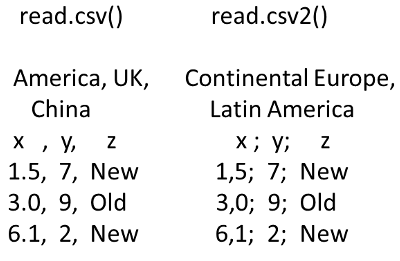
\includegraphics{csvFiles.png}
\caption{\label{fig:csvPlot}\emph{Illustration of the difference between two common forms of comma separated value (csv) files that can be read using the \texttt{read.csv()} and \texttt{read.csv2()} functions.}}
\end{figure}

Experience tells us that this is, unfortunately, not a trivial matter, because in some instances the two csv systems are mixed. For other file formats, the \texttt{read.table()} function provides additional flexibility. You can learn more about the options available by typing \texttt{?read.table}.

For our example above, if no error or warning messages appear then \texttt{R} has presumably read the irrigcorn.csv file, and stored the data in an object called \texttt{corn.dat}. To ensure the data was read successfully, use the\texttt{str()} function, \texttt{head()} function, or \texttt{summary()} function can be used, all producing different information.

\begin{Shaded}
\begin{Highlighting}[]
\KeywordTok{str}\NormalTok{(corn.dat)}
\end{Highlighting}
\end{Shaded}

\begin{verbatim}
## 'data.frame':    96 obs. of  8 variables:
##  $ Variety      : int  1 1 1 1 2 2 2 2 3 3 ...
##  $ Maturity     : int  92 92 92 92 86 86 86 86 84 84 ...
##  $ Irrig        : chr  "Full" "Full" "Full" "Full" ...
##  $ Population.A : int  23000 23000 23000 23000 23000 23000 23000 23000 23000 23000 ...
##  $ Population.ha: int  56810 56810 56810 56810 56810 56810 56810 56810 56810 56810 ...
##  $ Block        : int  1 2 3 4 1 2 3 4 1 2 ...
##  $ Yield.BuA    : int  202 163 186 178 177 176 179 168 172 150 ...
##  $ Yield.tonha  : num  12.7 10.2 11.7 11.2 11.1 ...
\end{verbatim}

The \texttt{str()} function provides information on the structure of the \texttt{R} object (and can be used with \emph{any} object, not just data frames). For data frames, the \texttt{str()} function will tell us the format for each column in the data frame. In the \texttt{corn.dat} data frame, we can see there are 96 rows and 8 columns, most of the columns contain interger (\texttt{int}) data, the `Irrig' variable is a character variable, and the last column is a numeric (\texttt{num}) variable.

\begin{Shaded}
\begin{Highlighting}[]
\KeywordTok{head}\NormalTok{(corn.dat)}
\end{Highlighting}
\end{Shaded}

\begin{verbatim}
##   Variety Maturity Irrig Population.A Population.ha Block Yield.BuA Yield.tonha
## 1       1       92  Full        23000         56810     1       202       12.68
## 2       1       92  Full        23000         56810     2       163       10.23
## 3       1       92  Full        23000         56810     3       186       11.68
## 4       1       92  Full        23000         56810     4       178       11.17
## 5       2       86  Full        23000         56810     1       177       11.11
## 6       2       86  Full        23000         56810     2       176       11.05
\end{verbatim}

The \texttt{head()} function shows the first few lines of the data set, and can be useful to ensure the data are structured correctly. However, the \texttt{head()} function does not allow you to see if a column of numbers is recognized as numbers or as characters. This is a common problem when reading in data from external files; if the csv or other data file is not properly formatted or contains strange characters (e.g. \texttt{”} or \texttt{;} or even letters), then the entire column will be recognized as a character or factor variable instead of a numeric variable. This is where the \texttt{str()} or \texttt{summary()} functions are helpful to recognize this problem.

In some cases, we may have a variable coded as an integer that we would like \texttt{R} to recognize as a factor variable. In the corn data set, the `Variety' variable is numbered, but there is no numeric order to the varieties. To convert this column to a factor variable, we can use the \texttt{as.factor()} function, and store the result as the same name as the original variable.

\begin{Shaded}
\begin{Highlighting}[]
\NormalTok{corn.dat}\OperatorTok{$}\NormalTok{Variety <-}\StringTok{ }\KeywordTok{as.factor}\NormalTok{(corn.dat}\OperatorTok{$}\NormalTok{Variety)}
\KeywordTok{str}\NormalTok{(corn.dat)}
\end{Highlighting}
\end{Shaded}

\begin{verbatim}
## 'data.frame':    96 obs. of  8 variables:
##  $ Variety      : Factor w/ 6 levels "1","2","3","4",..: 1 1 1 1 2 2 2 2 3 3 ...
##  $ Maturity     : int  92 92 92 92 86 86 86 86 84 84 ...
##  $ Irrig        : chr  "Full" "Full" "Full" "Full" ...
##  $ Population.A : int  23000 23000 23000 23000 23000 23000 23000 23000 23000 23000 ...
##  $ Population.ha: int  56810 56810 56810 56810 56810 56810 56810 56810 56810 56810 ...
##  $ Block        : int  1 2 3 4 1 2 3 4 1 2 ...
##  $ Yield.BuA    : int  202 163 186 178 177 176 179 168 172 150 ...
##  $ Yield.tonha  : num  12.7 10.2 11.7 11.2 11.1 ...
\end{verbatim}

Sometimes, despite all efforts to avoid the problem, numeric data is recognized by R as text, especially when exporting large data files from Excel or other spreadsheet software. This is sometimes due to spaces or other characters out of place in the data file; but sometimes the origin of the problem is difficult to find (especially with large data files). In these cases, one trick that can be tried is to convert the data to character, then back to numeric with the following code: \texttt{data\$var\ \textless{}-\ as.numeric(as.character(data\$var))}.

\begin{center}\rule{0.5\linewidth}{0.5pt}\end{center}

\hypertarget{welcome-to-the-tidyverse}{%
\chapter{Welcome to the Tidyverse}\label{welcome-to-the-tidyverse}}

The \href{https://www.tidyverse.org/}{\texttt{tidyverse} is a collection of packages} that were developed for data science. This group of packages provide some powerful and efficient functions that share a common syntax, making them seamless to use together. It is also possible (and common) to combine functions from the \texttt{tidyverse} with base \texttt{R} functions. The `tidy' in the name comes from the concept of \href{https://www.jstatsoft.org/index.php/jss/article/view/v059i10/v59i10.pdf}{tidy data}, which is basically a standardized way of managing data.

The \texttt{tidyverse} is a meta-package; the package itself does not contain any functions, but when you install or load \texttt{tidyverse} into your workspace, it ensures that the full group of packages are installed or loaded. The \texttt{tidyverse} includes three packages that we will use in this text (\texttt{dplyr}, \texttt{tidyr}, and \texttt{ggplot2}), plus several others.

\begin{Shaded}
\begin{Highlighting}[]
\KeywordTok{library}\NormalTok{(tidyverse)}
\end{Highlighting}
\end{Shaded}

\hypertarget{the-dplyr-package}{%
\section{\texorpdfstring{The \texttt{dplyr} package}{The dplyr package}}\label{the-dplyr-package}}

One of the most useful packages in the \texttt{tidyverse} is \texttt{dplyr}, and one of the most useful functions within the \texttt{tidyverse} is the pipe. Here, we will show how to use the pipe operator \texttt{\%\textgreater{}\%} to more efficiently do some of the same operations we showed in the previous chapter.

\hypertarget{the-dplyr-pipe}{%
\subsection{\texorpdfstring{The \texttt{dplyr} pipe (\texttt{\%\textgreater{}\%})}{The dplyr pipe (\%\textgreater{}\%)}}\label{the-dplyr-pipe}}

The concept of a pipe may be familiar to many programmers, but is often a new concept to scientists without a coding background. The simplest way to think about pipes is to say to yourself ``and then\ldots{}'' any time you see the pipe. One of the most common usages of pipes is illustrated below. In the first line, we specify which data we want to work with, \emph{and then} we perform operation 1, \emph{and then} we perform operation 2.

\begin{Shaded}
\begin{Highlighting}[]
\CommentTok{##  A common use of pipes (not run):}
\NormalTok{data.object }\OperatorTok
\StringTok{  }\NormalTok{operation }\DecValTok{1} \OperatorTok
\StringTok{  }\NormalTok{operation }\DecValTok{2}
\end{Highlighting}
\end{Shaded}

To illustrate, we will create some pretend data to use with \texttt{dplyr}. The data frame will be named `df', and will contain 20 rows and 4 columns. The \texttt{glimpse()} function from \texttt{dplyr} serves the same general purpose as \texttt{str()} when applied to data frames.

\begin{Shaded}
\begin{Highlighting}[]
\KeywordTok{set.seed}\NormalTok{(}\DecValTok{20102}\NormalTok{)}
\NormalTok{df1 <-}\StringTok{ }\KeywordTok{data.frame}\NormalTok{(}\DataTypeTok{fac =} \KeywordTok{rep}\NormalTok{(}\KeywordTok{c}\NormalTok{(}\StringTok{"A"}\NormalTok{,}\StringTok{"B"}\NormalTok{,}\StringTok{"C"}\NormalTok{,}\StringTok{"D"}\NormalTok{), }\DecValTok{5}\NormalTok{),}
                 \DataTypeTok{x =} \KeywordTok{c}\NormalTok{(}\DecValTok{1}\OperatorTok{:}\DecValTok{20}\NormalTok{),}
                 \DataTypeTok{y =} \KeywordTok{round}\NormalTok{(}\KeywordTok{rnorm}\NormalTok{(}\DecValTok{20}\NormalTok{, }\DecValTok{10}\NormalTok{, }\DecValTok{5}\NormalTok{)}\OperatorTok{*}\NormalTok{(}\OperatorTok{-}\DecValTok{9}\OperatorTok{:}\DecValTok{10}\NormalTok{)}\OperatorTok{^}\DecValTok{2}\NormalTok{),}
                 \DataTypeTok{z =} \KeywordTok{round}\NormalTok{(}\KeywordTok{rnorm}\NormalTok{(}\DecValTok{20}\NormalTok{, }\DecValTok{100}\NormalTok{, }\DecValTok{20}\NormalTok{)))}
\KeywordTok{glimpse}\NormalTok{(df1) }\CommentTok{# similar to the `str()` function in base R}
\end{Highlighting}
\end{Shaded}

\begin{verbatim}
## Rows: 20
## Columns: 4
## $ fac <chr> "A", "B", "C", "D", "A", "B", "C", "D", "A", "B", "C", "D", "A", "B", "C", "D", "A"...
## $ x   <int> 1, 2, 3, 4, 5, 6, 7, 8, 9, 10, 11, 12, 13, 14, 15, 16, 17, 18, 19, 20
## $ y   <dbl> 964, 625, 692, 309, 146, 174, 98, 63, 6, 0, 16, 49, 86, 208, 399, 258, 600, 546, 11...
## $ z   <dbl> 115, 110, 111, 92, 94, 107, 93, 95, 71, 100, 99, 75, 104, 92, 95, 75, 76, 88, 118, 104
\end{verbatim}

\hypertarget{group_by-and-summarize-functions}{%
\subsection{\texorpdfstring{\texttt{group\_by()} and \texttt{summarize()} functions}{group\_by() and summarize() functions}}\label{group_by-and-summarize-functions}}

One of the most useful things we can use dplyr for is to calculate descriptive statistics. For example, if we wanted to calculate the mean of y and z for the whole data set, we could use the \texttt{summarize()} function. This example takes the data frame `df', \emph{and then} uses the \texttt{summarize()} function to calculate the means of the columns named \emph{y} and \emph{z}.

\begin{Shaded}
\begin{Highlighting}[]
\CommentTok{### Using a pipe to calculate means.}
\NormalTok{df1 }\OperatorTok\StringTok{ }
\StringTok{  }\KeywordTok{summarize}\NormalTok{(}\DataTypeTok{y.mean =} \KeywordTok{mean}\NormalTok{(y),}
            \DataTypeTok{z.mean =} \KeywordTok{mean}\NormalTok{(z))}
\end{Highlighting}
\end{Shaded}

\begin{verbatim}
##   y.mean z.mean
## 1  416.9   95.7
\end{verbatim}

In this particular example, the pipe operator (\texttt{\%\textgreater{}\%}) isn't all that helpful. We could have gotten the same result more efficiently using several different methods. One method, still using the \texttt{summarize()} function, removes the pipe and adds the data frame as the first argument to the function:

\begin{Shaded}
\begin{Highlighting}[]
\CommentTok{### Doing the same thing without a pipe:}
\KeywordTok{summarize}\NormalTok{(df1, }
          \DataTypeTok{y.mean =} \KeywordTok{mean}\NormalTok{(y),}
          \DataTypeTok{z.mean =} \KeywordTok{mean}\NormalTok{(z))}
\end{Highlighting}
\end{Shaded}

\begin{verbatim}
##   y.mean z.mean
## 1  416.9   95.7
\end{verbatim}

But pipes become much more useful once we want to use multiple functions. To illustrate, we will combine two functions, the \texttt{group\_by()} and \texttt{summarize()} functions, in order to calculate means for different groups. If we assume the `fac' variable in the data is a treatment, and the y and z variables are responses to those treatments, then we will probably want to know the means for each treatment group. Using pipes, we can do that this way:

\begin{Shaded}
\begin{Highlighting}[]
\NormalTok{df1 }\OperatorTok
\StringTok{  }\KeywordTok{group_by}\NormalTok{(fac) }\OperatorTok
\StringTok{  }\KeywordTok{summarize}\NormalTok{(}\DataTypeTok{y.mean =} \KeywordTok{mean}\NormalTok{(y),}
            \DataTypeTok{z.mean =} \KeywordTok{mean}\NormalTok{(z))}
\end{Highlighting}
\end{Shaded}

\begin{verbatim}
## # A tibble: 4 x 3
##   fac   y.mean z.mean
##   <chr>  <dbl>  <dbl>
## 1 A       360.   92  
## 2 B       311.   99.4
## 3 C       479   103. 
## 4 D       518.   88.2
\end{verbatim}

This example starts with the data frame, \emph{and then} groups the data by levels in the `fac' column, \emph{and then} summarizes the data by calculating the means. It will be common to use summarized data in tables and figures, so we can also store this summarized data for later use (as in, perhaps, a bar plot):

\begin{Shaded}
\begin{Highlighting}[]
\NormalTok{df1.means <-}\StringTok{ }\NormalTok{df1 }\OperatorTok
\StringTok{  }\KeywordTok{group_by}\NormalTok{(fac) }\OperatorTok
\StringTok{  }\KeywordTok{summarize}\NormalTok{(}\DataTypeTok{y.mean =} \KeywordTok{mean}\NormalTok{(y),}
            \DataTypeTok{z.mean =} \KeywordTok{mean}\NormalTok{(z))}

\CommentTok{### Create a barplot of the means:}
\KeywordTok{barplot}\NormalTok{(df1.means}\OperatorTok{$}\NormalTok{y.mean, }\DataTypeTok{names.arg=}\NormalTok{df1.means}\OperatorTok{$}\NormalTok{fac, }\DataTypeTok{ylab=}\StringTok{"Y"}\NormalTok{)}
\end{Highlighting}
\end{Shaded}

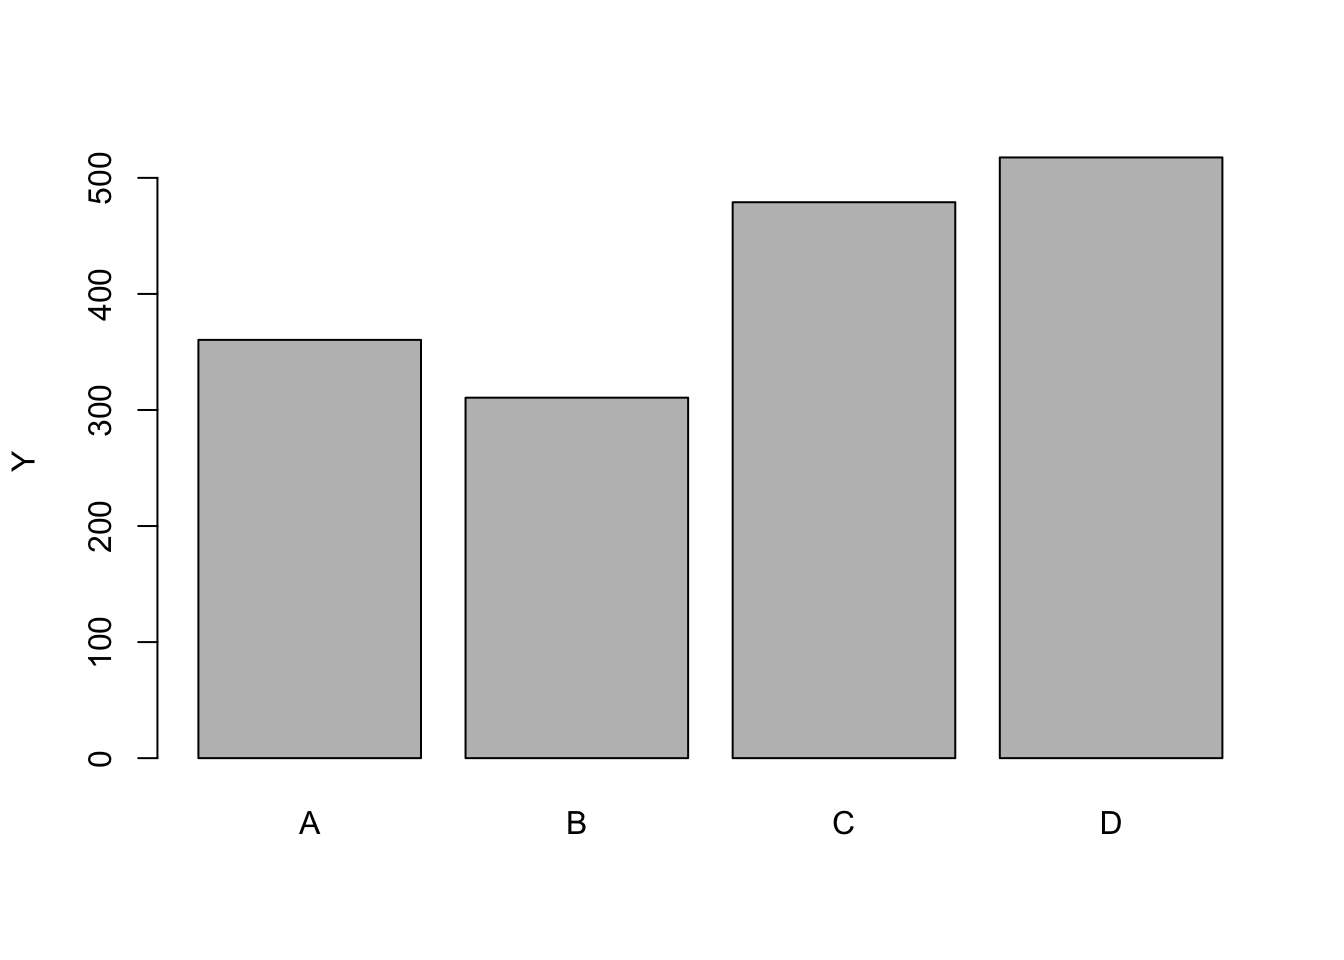
\includegraphics{Rstats4ag_files/figure-latex/unnamed-chunk-21-1.pdf}

\hypertarget{the-mutate-function}{%
\subsection{\texorpdfstring{The \texttt{mutate()} function}{The mutate() function}}\label{the-mutate-function}}

The \texttt{mutate()} function is used primarily when you want to create a new column. Common scenarios would include data transformations (such as log or square root), converting units (US customary units to SI units), or calculating a new variable for each observation from the measured data (calculating area from measured length and width). The syntax of \texttt{mutate} is similar to the \texttt{summarize()} function, but instead of reducing the data, it will keep the number of table rows the same while adding (or replacing) a column. For example, if we wanted to create a new variable that is the sum of \emph{y} and \emph{z} (named \emph{yz}):

\begin{Shaded}
\begin{Highlighting}[]
\NormalTok{df1.new <-}\StringTok{ }\NormalTok{df1 }\OperatorTok
\StringTok{  }\KeywordTok{mutate}\NormalTok{(}\DataTypeTok{yz =}\NormalTok{ y}\OperatorTok{+}\NormalTok{z)}
\KeywordTok{head}\NormalTok{(df1.new)}
\end{Highlighting}
\end{Shaded}

\begin{verbatim}
##   fac x   y   z   yz
## 1   A 1 964 115 1079
## 2   B 2 625 110  735
## 3   C 3 692 111  803
## 4   D 4 309  92  401
## 5   A 5 146  94  240
## 6   B 6 174 107  281
\end{verbatim}

Another powerful feature of \texttt{dplyr} is the ability to reference variables created earlier in the same function. For example, we can create the \emph{yz} variableas before, and then perform a transformation on the new variable, like taking the square root all within the same \texttt{mutate()} function:

\begin{Shaded}
\begin{Highlighting}[]
\NormalTok{df1.new <-}\StringTok{ }\NormalTok{df1 }\OperatorTok
\StringTok{  }\KeywordTok{mutate}\NormalTok{(}\DataTypeTok{yz =}\NormalTok{ y }\OperatorTok{+}\StringTok{ }\NormalTok{z,}
         \DataTypeTok{yz.sqrt =} \KeywordTok{sqrt}\NormalTok{(yz))}
\KeywordTok{head}\NormalTok{(df1.new)}
\end{Highlighting}
\end{Shaded}

\begin{verbatim}
##   fac x   y   z   yz  yz.sqrt
## 1   A 1 964 115 1079 32.84814
## 2   B 2 625 110  735 27.11088
## 3   C 3 692 111  803 28.33725
## 4   D 4 309  92  401 20.02498
## 5   A 5 146  94  240 15.49193
## 6   B 6 174 107  281 16.76305
\end{verbatim}

\hypertarget{filter-and-select-functions}{%
\subsection{\texorpdfstring{\texttt{filter()} and \texttt{select()} functions}{filter() and select() functions}}\label{filter-and-select-functions}}

\textless{}\textless{}\textless{}\textless{}\textless{}\textless{}\textless{} HEAD
The \texttt{filter()} and \texttt{select()} functions are useful for subsetting or removing rows or columns from your data. The \texttt{filter()} function is used to keep or remove \emph{rows} based on a specified criteria. For example, if we wanted to remove all rows with treatment `C' from the data, we could do so by filtering to \emph{keep} only rows where `fac' is not equal to `C'. The operator for `not equal' in \texttt{R} is \texttt{!=} (see table of useful operators at the end of this chapter).
=======
The \texttt{filter()} and \texttt{select()} functions are useful for subsetting or removing rows or columns from your data. The \texttt{filter()} function is used to keep or remove \emph{rows} based on a specified criteria. For example, if we wanted to remove all rows with treatment `C' from the data, we could do so by filtering to \emph{keep} only rows where `fac' is not equal to `C'. The operator for `not equal' in \texttt{R} is \texttt{!=}.
\textgreater{}\textgreater{}\textgreater{}\textgreater{}\textgreater{}\textgreater{}\textgreater{} 8e2378fe4699900a62ed1544c8f58ec178943c0c

\begin{Shaded}
\begin{Highlighting}[]
\NormalTok{df1.noC <-}\StringTok{ }\NormalTok{df1 }\OperatorTok
\StringTok{  }\KeywordTok{filter}\NormalTok{(fac }\OperatorTok{!=}\StringTok{ "C"}\NormalTok{)}
\NormalTok{df1.noC}
\end{Highlighting}
\end{Shaded}

\begin{verbatim}
##    fac  x    y   z
## 1    A  1  964 115
## 2    B  2  625 110
## 3    D  4  309  92
## 4    A  5  146  94
## 5    B  6  174 107
## 6    D  8   63  95
## 7    A  9    6  71
## 8    B 10    0 100
## 9    D 12   49  75
## 10   A 13   86 104
## 11   B 14  208  92
## 12   D 16  258  75
## 13   A 17  600  76
## 14   B 18  546  88
## 15   D 20 1909 104
\end{verbatim}

The behavior of \texttt{filter()} is to keep all rows that match whatever criteria we set in the function, so in the previous call, we keep all rows where \emph{fac} does \textbf{not} equal ``C''. We could also do the opposite, and keep only rows where the \emph{fac} variable is equal to \emph{C}. The operator for `equal to' in \texttt{R} is \texttt{==}.

\begin{Shaded}
\begin{Highlighting}[]
\NormalTok{df1.onlyC <-}\StringTok{ }\NormalTok{df1 }\OperatorTok
\StringTok{  }\KeywordTok{filter}\NormalTok{(fac }\OperatorTok{==}\StringTok{ "C"}\NormalTok{)}
\NormalTok{df1.onlyC}
\end{Highlighting}
\end{Shaded}

\begin{verbatim}
##   fac  x    y   z
## 1   C  3  692 111
## 2   C  7   98  93
## 3   C 11   16  99
## 4   C 15  399  95
## 5   C 19 1190 118
\end{verbatim}

Numeric values can be filtered similarly; for example if we want to keep only rows where `x' is \emph{less than or equal} to 8:

\begin{Shaded}
\begin{Highlighting}[]
\NormalTok{df1.u8 <-}\StringTok{ }\NormalTok{df1 }\OperatorTok
\StringTok{  }\KeywordTok{filter}\NormalTok{(x }\OperatorTok{<=}\StringTok{ }\DecValTok{8}\NormalTok{)}
\NormalTok{df1.u8}
\end{Highlighting}
\end{Shaded}

\begin{verbatim}
##   fac x   y   z
## 1   A 1 964 115
## 2   B 2 625 110
## 3   C 3 692 111
## 4   D 4 309  92
## 5   A 5 146  94
## 6   B 6 174 107
## 7   C 7  98  93
## 8   D 8  63  95
\end{verbatim}

And, like all things in dplyr, we can filter on multiple variables simultaneously. Perhaps for data quality checks, we want to look for all observations of treatment `C' where `y' is greater than 1,000. Note in this example, we use two equals signs `==' as the logical operator for `equal to', and we use the ampersand `\&' as the logical AND.

\begin{Shaded}
\begin{Highlighting}[]
\NormalTok{df1 }\OperatorTok
\StringTok{  }\KeywordTok{filter}\NormalTok{(y }\OperatorTok{>}\StringTok{ }\DecValTok{1000} \OperatorTok{&}\StringTok{ }\NormalTok{fac }\OperatorTok{==}\StringTok{ "C"}\NormalTok{)}
\end{Highlighting}
\end{Shaded}

\begin{verbatim}
##   fac  x    y   z
## 1   C 19 1190 118
\end{verbatim}

The `OR' operator in \texttt{R} is a vertical bar `\textbar{}'. So if we wanted to filter rows to keep all observations that are greater than 1,000 OR less than 100, we could use the following filter arguments:

\begin{Shaded}
\begin{Highlighting}[]
\NormalTok{df1 }\OperatorTok
\StringTok{  }\KeywordTok{filter}\NormalTok{(y }\OperatorTok{>}\StringTok{ }\DecValTok{1000} \OperatorTok{|}\StringTok{ }\NormalTok{y }\OperatorTok{<}\StringTok{ }\DecValTok{100}\NormalTok{)}
\end{Highlighting}
\end{Shaded}

\begin{verbatim}
##   fac  x    y   z
## 1   C  7   98  93
## 2   D  8   63  95
## 3   A  9    6  71
## 4   B 10    0 100
## 5   C 11   16  99
## 6   D 12   49  75
## 7   A 13   86 104
## 8   C 19 1190 118
## 9   D 20 1909 104
\end{verbatim}

The \texttt{select()} function provides similar ability but for columns instead of rows. We can keep variables by including the column names in the \texttt{select()} function, and we can remove them by using a `-' sign in front of the name (but typically using one or the other, not both). The following examples will result in the same three columns being retained, just \emph{fac}, \emph{x}, and \emph{y}. In the first, we will explicitly include these three columns by naming them. In the second example, we will exclude the \emph{z} column by using the minus sign.

\begin{Shaded}
\begin{Highlighting}[]
\CommentTok{### Example 1 - keeping columns}
\NormalTok{df1 }\OperatorTok
\StringTok{  }\KeywordTok{select}\NormalTok{(fac, x, y) }\OperatorTok
\StringTok{  }\KeywordTok{head}\NormalTok{()}
\end{Highlighting}
\end{Shaded}

\begin{verbatim}
##   fac x   y
## 1   A 1 964
## 2   B 2 625
## 3   C 3 692
## 4   D 4 309
## 5   A 5 146
## 6   B 6 174
\end{verbatim}

\begin{Shaded}
\begin{Highlighting}[]
\CommentTok{### Example 2 - removing a column}
\NormalTok{df1 }\OperatorTok\StringTok{ }
\StringTok{  }\KeywordTok{select}\NormalTok{(}\OperatorTok{-}\NormalTok{z) }\OperatorTok
\StringTok{  }\KeywordTok{head}\NormalTok{()}
\end{Highlighting}
\end{Shaded}

\begin{verbatim}
##   fac x   y
## 1   A 1 964
## 2   B 2 625
## 3   C 3 692
## 4   D 4 309
## 5   A 5 146
## 6   B 6 174
\end{verbatim}

\hypertarget{the-tidyr-package}{%
\section{\texorpdfstring{The \texttt{tidyr} package}{The tidyr package}}\label{the-tidyr-package}}

Another package contained in the \texttt{tidyverse} is \texttt{tidyr}. This package, as you might suspect form the name, relates to the tidy data format \href{https://vita.had.co.nz/papers/tidy-data.pdf}{Wickham 2014}. The two functions that we will use are called \texttt{pivot\_longer()} which takes a `wide' data set and reformats it to the long format, and \texttt{pivot\_wider()} which takes a long data format and reformats it to a wider version. To begin, we'll create some pretend data in the wide format:

\begin{Shaded}
\begin{Highlighting}[]
\KeywordTok{set.seed}\NormalTok{(}\DecValTok{4070}\NormalTok{)}
\NormalTok{df.wide <-}\StringTok{ }\KeywordTok{data.frame}\NormalTok{(}
  \DataTypeTok{replicate =} \DecValTok{1}\OperatorTok{:}\DecValTok{6}\NormalTok{,}
  \DataTypeTok{trt1 =} \KeywordTok{round}\NormalTok{(}\KeywordTok{rnorm}\NormalTok{(}\DecValTok{6}\NormalTok{, }\DecValTok{10}\NormalTok{, }\DecValTok{1}\NormalTok{),}\DecValTok{1}\NormalTok{),}
  \DataTypeTok{trt2 =} \KeywordTok{round}\NormalTok{(}\KeywordTok{rnorm}\NormalTok{(}\DecValTok{6}\NormalTok{, }\DecValTok{13}\NormalTok{, }\DecValTok{1}\NormalTok{),}\DecValTok{1}\NormalTok{),}
  \DataTypeTok{trt3 =} \KeywordTok{round}\NormalTok{(}\KeywordTok{rnorm}\NormalTok{(}\DecValTok{6}\NormalTok{, }\DecValTok{4}\NormalTok{, }\DecValTok{1}\NormalTok{),}\DecValTok{1}\NormalTok{))}
\end{Highlighting}
\end{Shaded}

To see what the data looks like in wide format, we can print the \texttt{df.wide} data frame we just created:

\begin{Shaded}
\begin{Highlighting}[]
\NormalTok{df.wide}
\end{Highlighting}
\end{Shaded}

\begin{verbatim}
##   replicate trt1 trt2 trt3
## 1         1 11.2 13.9  4.8
## 2         2  8.5 13.9  3.8
## 3         3  8.4 13.1  3.7
## 4         4  8.9 12.9  5.1
## 5         5 10.7 13.5  3.0
## 6         6 11.1 14.3  4.3
\end{verbatim}

To convert this wide data into the long format that is typically preferred for statistical analysis, we can use the \texttt{pivot\_longer()} function. For a simple data frame like this, there are four arguments we need to provide:

\begin{enumerate}
\def\labelenumi{\arabic{enumi}.}
\tightlist
\item
  the \texttt{data} argument, which tells R which data frame we'll be starting with;
\item
  the \texttt{cols} argument, which a list of columns we don't want to gather from wide to long format;
\item
  the \texttt{names\_to} argument, which is what we want the column that contains the treatment information to be named; and
\item
  the \texttt{values\_to} argument, which is what we want to name the column that contains the data.
\end{enumerate}

For this example, the data we are using is called `df.wide'. The columns we don't want to include are any `housekeeping' variables; in this case it is only one column, named `replicate'. We will store the treatment in a new column named `treatment', and we will put the data into a new column named `weight'. So the \texttt{pivot\_longer()} function would look like this:

\begin{Shaded}
\begin{Highlighting}[]
\NormalTok{df.long <-}\StringTok{ }\KeywordTok{pivot_longer}\NormalTok{(}\DataTypeTok{data =}\NormalTok{ df.wide,}
                        \DataTypeTok{cols =} \OperatorTok{-}\NormalTok{replicate, }
                        \DataTypeTok{names_to =} \StringTok{"treatment"}\NormalTok{, }
                        \DataTypeTok{values_to =} \StringTok{"weight"}\NormalTok{)}
\NormalTok{df.long}
\end{Highlighting}
\end{Shaded}

\begin{verbatim}
## # A tibble: 18 x 3
##    replicate treatment weight
##        <int> <chr>      <dbl>
##  1         1 trt1        11.2
##  2         1 trt2        13.9
##  3         1 trt3         4.8
##  4         2 trt1         8.5
##  5         2 trt2        13.9
##  6         2 trt3         3.8
##  7         3 trt1         8.4
##  8         3 trt2        13.1
##  9         3 trt3         3.7
## 10         4 trt1         8.9
## 11         4 trt2        12.9
## 12         4 trt3         5.1
## 13         5 trt1        10.7
## 14         5 trt2        13.5
## 15         5 trt3         3  
## 16         6 trt1        11.1
## 17         6 trt2        14.3
## 18         6 trt3         4.3
\end{verbatim}

We could also use the `pipes' from \texttt{dplyr} as in the previous example to achieve the same result:

\begin{Shaded}
\begin{Highlighting}[]
\NormalTok{df.long <-}\StringTok{ }\NormalTok{df.wide }\OperatorTok
\StringTok{  }\KeywordTok{pivot_longer}\NormalTok{(}\DataTypeTok{cols =} \OperatorTok{-}\NormalTok{replicate,}
               \DataTypeTok{names_to =} \StringTok{"treatment"}\NormalTok{,}
               \DataTypeTok{values_to =} \StringTok{"weight"}\NormalTok{)}
\end{Highlighting}
\end{Shaded}

In this example, there is no real benefit for using the pipes. However, if we wanted to do more operations on the same data, like filter or summarize the data, then the efficiency of pipes becomes substantial. For example, if we wanted to convert the weight from pounds to kilograms, and then summarize the data by treatment, we could use the following code:

\begin{Shaded}
\begin{Highlighting}[]
\NormalTok{df.wide }\OperatorTok
\StringTok{  }\KeywordTok{pivot_longer}\NormalTok{(}\DataTypeTok{cols =} \OperatorTok{-}\NormalTok{replicate,}
               \DataTypeTok{names_to =} \StringTok{"treatment"}\NormalTok{,}
               \DataTypeTok{values_to =} \StringTok{"weight"}\NormalTok{) }\OperatorTok
\StringTok{  }\KeywordTok{mutate}\NormalTok{(}\DataTypeTok{weight.kg =}\NormalTok{ weight }\OperatorTok{*}\StringTok{ }\FloatTok{0.4536}\NormalTok{) }\OperatorTok
\StringTok{  }\KeywordTok{group_by}\NormalTok{(treatment) }\OperatorTok
\StringTok{  }\KeywordTok{summarize}\NormalTok{(}\DataTypeTok{meanWeight.kg =} \KeywordTok{mean}\NormalTok{(weight.kg))}
\end{Highlighting}
\end{Shaded}

\begin{verbatim}
## # A tibble: 3 x 2
##   treatment meanWeight.kg
##   <chr>             <dbl>
## 1 trt1               4.45
## 2 trt2               6.17
## 3 trt3               1.87
\end{verbatim}

It is also possible to use pipes with base \texttt{R} functions. One useful implementation of this is to mutate (or group or summarize) data as part of the input process. For example, we can read the data file in with \texttt{read.csv}, then pipe various other functions so that the data is in the correct format for analysis right from the start. For example, the following code will get the data, use the \texttt{mutate()} function to convert a blocking variable to a factor and transform a response variable with a log transformation, then pass that to the \texttt{filter()} function to remove one year of data (2009):

\begin{Shaded}
\begin{Highlighting}[]
\NormalTok{beanDat <-}\StringTok{ }\KeywordTok{read.csv}\NormalTok{(}\StringTok{"http://rstats4ag.org/data/FlumiBeans.csv"}\NormalTok{) }\OperatorTok
\StringTok{  }\KeywordTok{mutate}\NormalTok{(}\DataTypeTok{block =} \KeywordTok{factor}\NormalTok{(block),}
         \DataTypeTok{logDensity =} \KeywordTok{log}\NormalTok{(population}\FloatTok{.4}\NormalTok{wk)) }\OperatorTok
\StringTok{  }\KeywordTok{filter}\NormalTok{(year }\OperatorTok{!=}\StringTok{ }\DecValTok{2009}\NormalTok{)}
\KeywordTok{glimpse}\NormalTok{(beanDat)}
\end{Highlighting}
\end{Shaded}

\begin{verbatim}
## Rows: 56
## Columns: 5
## $ year           <int> 2010, 2010, 2010, 2010, 2010, 2010, 2010, 2010, 2010, 2010, 2010, 2010, ...
## $ treatment      <chr> "Nontreated", "Nontreated", "Nontreated", "Nontreated", "flumioxazin + t...
## $ block          <fct> 1, 2, 3, 4, 1, 2, 3, 4, 1, 2, 3, 4, 1, 2, 3, 4, 1, 2, 3, 4, 1, 2, 3, 4, ...
## $ population.4wk <int> 45302, 52272, 55757, 48787, 10454, 41818, 10454, 20909, 17424, 17424, 20...
## $ logDensity     <dbl> 10.721106, 10.864216, 10.928758, 10.795219, 9.254740, 10.641082, 9.25474...
\end{verbatim}

\begin{center}\rule{0.5\linewidth}{0.5pt}\end{center}

\textbf{Table of useful operators in the \texttt{R} language.}

\begin{tabular}{l|l}
\hline
operator & meaning\\
\hline
== & equal to\\
\hline
!= & not equal to\\
\hline
> & greater than\\
\hline
>= & greater than or equal to\\
\hline
< & less than\\
\hline
<= & less than or equal to\\
\hline
\& & and\\
\hline
| & or\\
\hline
\end{tabular}

\hypertarget{descriptive-statistics}{%
\chapter{Descriptive Statistics}\label{descriptive-statistics}}

\hypertarget{calculating-group-means}{%
\section{Calculating group means}\label{calculating-group-means}}

One of the most basic exploratory tasks with any data set involves computing the mean, variance, and other descriptive statistics. A previous section has already demonstrated how to obtain many of these statistics from a data set, using the \texttt{summary()}, \texttt{mean()}, and \texttt{sd()} functions. However these functions were used in the context of an entire data set or column from a data set; in most cases it will be more informative to calculate these statistics for groups of data, such as experimental treatments. The \texttt{tapply()} function can be used for this purpose. Summary statistics for the corn irrigation data set were calculated previously using the \texttt{summary()} function. The \texttt{tapply()} function allows us to calculate similar descriptive statistics for groups of data, most commonly for treatments, but also for other logical groups, such as by experimental sites, or years. The \texttt{tapply()} function requires three arguments:

\begin{itemize}
\tightlist
\item
  The data column you want to summarize (response variable)
\item
  The data column you wish to group the data by (treatment or grouping variable)
\item
  The function you want to calculate (mean, standard deviation, maximum, etc.)
\end{itemize}

The example below will calculate mean yield for each irrigation block (Full irrigation or Limited irrigation).

\begin{Shaded}
\begin{Highlighting}[]
\NormalTok{corn.dat <-}\StringTok{ }\KeywordTok{read.csv}\NormalTok{(}\StringTok{"http://rstats4ag.org/data/irrigcorn.csv"}\NormalTok{)}
\KeywordTok{tapply}\NormalTok{(corn.dat}\OperatorTok{$}\NormalTok{Yield.BuA, corn.dat}\OperatorTok{$}\NormalTok{Irrig, mean)}
\end{Highlighting}
\end{Shaded}

\begin{verbatim}
##     Full  Limited 
## 181.1667 163.2708
\end{verbatim}

To specify multiple grouping variables, we use the \texttt{list()} function within the \texttt{tapply()} function:

\begin{Shaded}
\begin{Highlighting}[]
\KeywordTok{tapply}\NormalTok{(corn.dat}\OperatorTok{$}\NormalTok{Yield.BuA, }\KeywordTok{list}\NormalTok{(corn.dat}\OperatorTok{$}\NormalTok{Population.A, corn.dat}\OperatorTok{$}\NormalTok{Irrig), mean)}
\end{Highlighting}
\end{Shaded}

\begin{verbatim}
##           Full  Limited
## 23000 171.1667 147.3333
## 33000 191.1667 179.2083
\end{verbatim}

\hypertarget{calculating-other-group-statistics-with-tapply}{%
\section{Calculating other group statistics with tapply}\label{calculating-other-group-statistics-with-tapply}}

We can use the same syntax to calculate nearly any statistic for the groups by replacing the \texttt{mean} argument with another function, such as \texttt{max}, \texttt{min}, \texttt{sd} etc.

\begin{Shaded}
\begin{Highlighting}[]
\KeywordTok{tapply}\NormalTok{(corn.dat}\OperatorTok{$}\NormalTok{Yield.BuA, }\KeywordTok{list}\NormalTok{(corn.dat}\OperatorTok{$}\NormalTok{Population.A, corn.dat}\OperatorTok{$}\NormalTok{Irrig), median)}
\end{Highlighting}
\end{Shaded}

\begin{verbatim}
##       Full Limited
## 23000  171   152.5
## 33000  191   182.5
\end{verbatim}

You can also specify other functions or operations. For example, there is no default function in \texttt{R} to calculate the CV, or coefficient of variation. This statistic is commonly used in crop sciences. The CV is simply the standard deviation divided by the mean, and so we can calculate the CV using by storing the output from \texttt{tapply()} into an object that we can call upon later.

\begin{Shaded}
\begin{Highlighting}[]
\NormalTok{popirr.sd   <-}\StringTok{ }\KeywordTok{tapply}\NormalTok{(corn.dat}\OperatorTok{$}\NormalTok{Yield.BuA, }
                      \KeywordTok{list}\NormalTok{(corn.dat}\OperatorTok{$}\NormalTok{Population.A, corn.dat}\OperatorTok{$}\NormalTok{Irrig), sd)}
\NormalTok{popirr.mean <-}\StringTok{ }\KeywordTok{tapply}\NormalTok{(corn.dat}\OperatorTok{$}\NormalTok{Yield.BuA, }
                      \KeywordTok{list}\NormalTok{(corn.dat}\OperatorTok{$}\NormalTok{Population.A, corn.dat}\OperatorTok{$}\NormalTok{Irrig), mean)}
\NormalTok{popirr.cv<-popirr.sd}\OperatorTok{/}\NormalTok{popirr.mean}
\KeywordTok{round}\NormalTok{(popirr.cv, }\DecValTok{3}\NormalTok{)}
\end{Highlighting}
\end{Shaded}

\begin{verbatim}
##        Full Limited
## 23000 0.075   0.102
## 33000 0.052   0.098
\end{verbatim}

The \texttt{round()} function simply rounds the result to 3 decimal places to make the output more readable. Alternatively, if the CV is a statistic we will use regularly, it may be worthwhile to write our own function to save keystrokes later on. We can do this using \texttt{function()}.

\begin{Shaded}
\begin{Highlighting}[]
\NormalTok{cv <-}\StringTok{ }\ControlFlowTok{function}\NormalTok{(x) \{}
\NormalTok{  xm  <-}\StringTok{ }\KeywordTok{mean}\NormalTok{(x)}
\NormalTok{  xsd <-}\StringTok{ }\KeywordTok{sd}\NormalTok{(x)}
\NormalTok{  xcv <-}\StringTok{ }\NormalTok{xsd}\OperatorTok{/}\NormalTok{xm}
  \KeywordTok{round}\NormalTok{(xcv, }\DecValTok{4}\NormalTok{)}
\NormalTok{\}}
\end{Highlighting}
\end{Shaded}

Or, more efficiently:

\begin{Shaded}
\begin{Highlighting}[]
\NormalTok{cv <-}\StringTok{ }\ControlFlowTok{function}\NormalTok{(x) \{}
\NormalTok{  xcv <-}\StringTok{ }\KeywordTok{round}\NormalTok{(}\KeywordTok{sd}\NormalTok{(x) }\OperatorTok{/}\StringTok{ }\KeywordTok{mean}\NormalTok{(x), }\DecValTok{4}\NormalTok{)}
\NormalTok{\}}
\KeywordTok{tapply}\NormalTok{(corn.dat}\OperatorTok{$}\NormalTok{Yield.BuA, }\KeywordTok{list}\NormalTok{(corn.dat}\OperatorTok{$}\NormalTok{Population.A, corn.dat}\OperatorTok{$}\NormalTok{Irrig), cv)}
\end{Highlighting}
\end{Shaded}

\begin{verbatim}
##         Full Limited
## 23000 0.0750  0.1021
## 33000 0.0523  0.0976
\end{verbatim}

This approach is desirable if the CV will be used repeatedly. Once the function \texttt{cv()} has been defined, you can call upon it repeatedly with very few keystrokes.

\hypertarget{using-dplyr-to-summarize-data}{%
\section{Using dplyr to summarize data}\label{using-dplyr-to-summarize-data}}

In addition to using \texttt{tapply()} from base stats R package, there is an excellent package for summarizing data called \texttt{dplyr}. We can get similar information from the corn data set using the \texttt{dplyr} package using the following syntax (explained in more detail below).

\begin{Shaded}
\begin{Highlighting}[]
\KeywordTok{library}\NormalTok{(dplyr)}
\NormalTok{corn.summary <-}\StringTok{ }\NormalTok{corn.dat }\OperatorTok
\StringTok{  }\KeywordTok{group_by}\NormalTok{(Population.A, Irrig) }\OperatorTok
\StringTok{  }\KeywordTok{summarize}\NormalTok{(}\DataTypeTok{N        =} \KeywordTok{length}\NormalTok{(Yield.BuA),}
            \DataTypeTok{AvgYield =} \KeywordTok{round}\NormalTok{(}\KeywordTok{mean}\NormalTok{(Yield.BuA),}\DecValTok{1}\NormalTok{),}
            \DataTypeTok{CV       =} \KeywordTok{cv}\NormalTok{(Yield.BuA))}
\NormalTok{corn.summary            }
\end{Highlighting}
\end{Shaded}

\begin{verbatim}
## # A tibble: 4 x 5
## # Groups:   Population.A [2]
##   Population.A Irrig       N AvgYield     CV
##          <int> <chr>   <int>    <dbl>  <dbl>
## 1        23000 Full       24     171. 0.075 
## 2        23000 Limited    24     147. 0.102 
## 3        33000 Full       24     191. 0.0523
## 4        33000 Limited    24     179. 0.0976
\end{verbatim}

We will explain and demonstrate some of the basic uses of \texttt{dplyr} using herbicide resistant weed data from Canada. The following data set was assembled using data from \href{http://www.weedscience.org}{weedscience.org}.

\begin{Shaded}
\begin{Highlighting}[]
\NormalTok{resistance<-}\KeywordTok{read.csv}\NormalTok{(}\StringTok{"http://rstats4ag.org/data/CanadaResistance2.csv"}\NormalTok{)}
\NormalTok{resistance<-}\KeywordTok{na.omit}\NormalTok{(resistance)}
\KeywordTok{head}\NormalTok{(resistance)}
\end{Highlighting}
\end{Shaded}

\begin{verbatim}
##   Province ID          SciName Year                                     MOA
## 1  Alberta  1  Stellaria media 1988                    ALS inhibitors (B/2)
## 2  Alberta  2  Kochia scoparia 1989                    ALS inhibitors (B/2)
## 3  Alberta  3      Avena fatua 1989 Multiple Resistance: 2 Sites of Action 
## 6  Alberta  4  Setaria viridis 1989           Microtubule inhibitors (K1/3)
## 7  Alberta  5      Avena fatua 1991                 ACCase inhibitors (A/1)
## 8  Alberta  6 Sinapis arvensis 1993                    ALS inhibitors (B/2)
\end{verbatim}

In the data file, there are instances of multiple resistance (resistance to more than one mode of action).
The second line of the code above (\texttt{na.omit()}) removes all lines in the data set that contain \texttt{NA} (which is the default value in R for missing data). This is necessary for this particular example so that instances of multiple resistance are not counted multiple times. We may want to use the information from those rows later on, however, and therefore this method is preferable to deleting the rows from the raw data file.

One of the first things we might like to do is simply count the number of herbicide resistant weed cases by mode of action. We could do this rather quickly using the \texttt{tapply()} function discussed in the previous section: \texttt{tapply(resistance\$ID,\ resistance\$MOA,\ length)}. In the code below, we will use the \texttt{dplyr} package to get some interesting information from this data set. First, we can simply count the number of herbicide resistant weeds for each mode of action in the data set. Initially it seems like much more typing compared to using \texttt{tapply()}, but later on it will become clear why this is a potentially more powerful method.

\begin{Shaded}
\begin{Highlighting}[]
\KeywordTok{library}\NormalTok{(dplyr)}
\NormalTok{bymoa<-}\KeywordTok{group_by}\NormalTok{(resistance, MOA)}
\NormalTok{moatotal<-}\KeywordTok{summarize}\NormalTok{(bymoa, }\DataTypeTok{total=}\KeywordTok{length}\NormalTok{(ID))}
\KeywordTok{print}\NormalTok{(moatotal)}
\end{Highlighting}
\end{Shaded}

In the code above, we are loading the dplyr package, then using two functions from that package. The \texttt{group\_by()} function will provide the information on how the data are grouped. In this case, we want to group the data by MOA. We can then use the the \texttt{summarize()} function to calculate means, counts, sums, or any other operation on the data. Above, we used the \texttt{length()} function to count the unique instances of the ID variable for each mode of action. Storing each step with the \texttt{\textless{}-} operator can be a little cumbersome, especially if we will not need to use the intermediary steps again. The \texttt{dplyr} package uses the \texttt{\%\textgreater{}\%} operator to string together several steps. The code below will result in the same summary as above, with fewer keystrokes, and without storing the intermediary grouping as a separate object. The first line provides the name of the data set (\texttt{resistance}) followed by the \texttt{\%\textgreater{}\%} operator. This tells \texttt{R} to expect a function on the next line from the dplyr package. The second line groups the resistance data set by MOA, and the third line summarizes the data by calculating the length of the ID variable for each level of the grouping factor. Effectively, this counts each instance of resistance. The last line prints out the resulting data frame.

\begin{Shaded}
\begin{Highlighting}[]
\NormalTok{moatotal <-}\StringTok{ }\NormalTok{resistance }\OperatorTok
\StringTok{  }\KeywordTok{group_by}\NormalTok{(MOA) }\OperatorTok
\StringTok{  }\KeywordTok{summarize}\NormalTok{(}\DataTypeTok{total=}\KeywordTok{length}\NormalTok{(ID))}
\NormalTok{moatotal}
\end{Highlighting}
\end{Shaded}

\begin{verbatim}
## # A tibble: 13 x 2
##    MOA                                        total
##    <chr>                                      <int>
##  1 "ACCase inhibitors (A/1)"                      9
##  2 "ALS inhibitors (B/2)"                        42
##  3 "EPSP synthase inhibitors (G/9)"               2
##  4 "Lipid Inhibitors (thiocarbamates) (N/8)"      2
##  5 "Microtubule inhibitors (K1/3)"                3
##  6 "Multiple Resistance: 2 Sites of Action "     12
##  7 "Multiple Resistance: 3 Sites of Action "      3
##  8 "Multiple Resistance: 4 Sites of Action "      1
##  9 "Photosystem II inhibitors (C1/5)"            12
## 10 "PSI Electron Diverter (D/22)"                 3
## 11 "PSII inhibitor (Ureas and amides) (C2/7)"     3
## 12 "PSII inhibitors (Nitriles) (C3/6)"            2
## 13 "Synthetic Auxins (O/4)"                       3
\end{verbatim}

The real power and elegance of the \texttt{dplyr} package becomes apparent once we begin using multiple groupings, and creating new variables. Below, we generate totals for each mode of action again, but also by year of listing by using the \texttt{group\_by()} and \texttt{sumarize()} functions.

\begin{Shaded}
\begin{Highlighting}[]
\NormalTok{totals <-}\StringTok{ }\NormalTok{resistance }\OperatorTok
\StringTok{  }\KeywordTok{group_by}\NormalTok{(Year, MOA) }\OperatorTok
\StringTok{  }\KeywordTok{summarize}\NormalTok{(}\DataTypeTok{total =} \KeywordTok{length}\NormalTok{(ID)) }
\KeywordTok{head}\NormalTok{(totals)}
\end{Highlighting}
\end{Shaded}

\begin{verbatim}
## # A tibble: 6 x 3
## # Groups:   Year [6]
##    Year MOA                              total
##   <int> <chr>                            <int>
## 1  1957 Synthetic Auxins (O/4)               1
## 2  1973 Photosystem II inhibitors (C1/5)     1
## 3  1976 Photosystem II inhibitors (C1/5)     2
## 4  1977 Photosystem II inhibitors (C1/5)     3
## 5  1980 Photosystem II inhibitors (C1/5)     1
## 6  1981 Photosystem II inhibitors (C1/5)     3
\end{verbatim}

\begin{Shaded}
\begin{Highlighting}[]
\KeywordTok{tail}\NormalTok{(totals)}
\end{Highlighting}
\end{Shaded}

\begin{verbatim}
## # A tibble: 6 x 3
## # Groups:   Year [3]
##    Year MOA                                       total
##   <int> <chr>                                     <int>
## 1  2010 "EPSP synthase inhibitors (G/9)"              1
## 2  2011 "ACCase inhibitors (A/1)"                     1
## 3  2011 "ALS inhibitors (B/2)"                        2
## 4  2011 "Multiple Resistance: 2 Sites of Action "     2
## 5  2012 "ALS inhibitors (B/2)"                        1
## 6  2012 "Multiple Resistance: 2 Sites of Action "     3
\end{verbatim}

We can then create a new variable using the \texttt{mutate()} function; we will add a cumulative total of herbicide resistance cases over time, while retaining information about mode of action by first ungrouping the data, then using mutate to calculate the cumulative total using the \texttt{cumsum()} from the default stats package.

\begin{Shaded}
\begin{Highlighting}[]
\NormalTok{totals <-}\StringTok{ }\NormalTok{resistance }\OperatorTok
\StringTok{  }\KeywordTok{group_by}\NormalTok{(Year, MOA) }\OperatorTok
\StringTok{  }\KeywordTok{summarize}\NormalTok{(}\DataTypeTok{total =} \KeywordTok{length}\NormalTok{(ID)) }\OperatorTok
\StringTok{  }\KeywordTok{ungroup}\NormalTok{() }\OperatorTok
\StringTok{  }\KeywordTok{mutate}\NormalTok{(}\DataTypeTok{cumulative =} \KeywordTok{cumsum}\NormalTok{(total))}
\KeywordTok{head}\NormalTok{(totals)}
\end{Highlighting}
\end{Shaded}

\begin{verbatim}
## # A tibble: 6 x 4
##    Year MOA                              total cumulative
##   <int> <chr>                            <int>      <int>
## 1  1957 Synthetic Auxins (O/4)               1          1
## 2  1973 Photosystem II inhibitors (C1/5)     1          2
## 3  1976 Photosystem II inhibitors (C1/5)     2          4
## 4  1977 Photosystem II inhibitors (C1/5)     3          7
## 5  1980 Photosystem II inhibitors (C1/5)     1          8
## 6  1981 Photosystem II inhibitors (C1/5)     3         11
\end{verbatim}

\begin{Shaded}
\begin{Highlighting}[]
\KeywordTok{tail}\NormalTok{(totals)}
\end{Highlighting}
\end{Shaded}

\begin{verbatim}
## # A tibble: 6 x 4
##    Year MOA                                       total cumulative
##   <int> <chr>                                     <int>      <int>
## 1  2010 "EPSP synthase inhibitors (G/9)"              1         88
## 2  2011 "ACCase inhibitors (A/1)"                     1         89
## 3  2011 "ALS inhibitors (B/2)"                        2         91
## 4  2011 "Multiple Resistance: 2 Sites of Action "     2         93
## 5  2012 "ALS inhibitors (B/2)"                        1         94
## 6  2012 "Multiple Resistance: 2 Sites of Action "     3         97
\end{verbatim}

We can also use \texttt{dplyr} to look at other grouping, including by province or weed species, and then use the \texttt{subset()} function to print out only one group. In the below example, we will calculate totals for each province by weed species then keep only the cases from Saskatchewan.

\begin{Shaded}
\begin{Highlighting}[]
\NormalTok{resistance.SK <-}\StringTok{ }\NormalTok{resistance }\OperatorTok
\StringTok{  }\KeywordTok{group_by}\NormalTok{(Province, SciName) }\OperatorTok
\StringTok{  }\KeywordTok{summarize}\NormalTok{(}\DataTypeTok{total=}\KeywordTok{length}\NormalTok{(ID)) }\OperatorTok
\StringTok{  }\KeywordTok{filter}\NormalTok{(Province }\OperatorTok{==}\StringTok{ "Saskatchewan"}\NormalTok{) }\OperatorTok
\StringTok{  }\KeywordTok{arrange}\NormalTok{(}\OperatorTok{-}\NormalTok{total) }
\NormalTok{resistance.SK}
\end{Highlighting}
\end{Shaded}

\begin{verbatim}
## # A tibble: 12 x 3
## # Groups:   Province [1]
##    Province     SciName                 total
##    <chr>        <chr>                   <int>
##  1 Saskatchewan Avena fatua                 4
##  2 Saskatchewan Setaria viridis             3
##  3 Saskatchewan Kochia scoparia             2
##  4 Saskatchewan Amaranthus retroflexus      1
##  5 Saskatchewan Capsella bursa-pastoris     1
##  6 Saskatchewan Chenopodium album           1
##  7 Saskatchewan Galium spurium              1
##  8 Saskatchewan Lolium persicum             1
##  9 Saskatchewan Salsola tragus              1
## 10 Saskatchewan Sinapis arvensis            1
## 11 Saskatchewan Stellaria media             1
## 12 Saskatchewan Thlaspi arvense             1
\end{verbatim}

\begin{center}\rule{0.5\linewidth}{0.5pt}\end{center}

\hypertarget{simple-correlation}{%
\chapter{Simple Correlation}\label{simple-correlation}}

To quantify relationships between quantitative treatment structures (such as increasing rates) and a response variable, regression analysis is most appropriate. But in many cases it is of interest to determine the strength of a relationship between two measured variables (where no cause-effect or dose-response relationship is obvious). This can most easily be done with correlation analysis. Examples where correlation analysis would be appropriate include observational studies where soil texture (e.g.~percent clay content) is thought to be related to density of a particular weed species; or the amount of sunlight reaching the crop canopy is related to crop biomass. In these cases, experimental treatments may not be explicitly designed, but rather many areas of a field could be sampled for both variables, and the correlation analysis conducted to quantify the strength of the relationship.

The relationship between visual assessment of crop injury and dry weight (or yield) production of a crop may also be of interest to a researcher. This would not be a cause-effect relationship (injury symptoms do not cause dry weight reduction), and therefore correlation analysis is more appropriate than regression. In a study by Lyon and Kniss (2010), proso millet was tested for its tolerance to preemergence applications of the herbicide saflufenacil. Injury to the crop was evaluated visually at 10 and 20 days after treatment, and dry weight was measured 28 days after treatment. It is expected that visual injury symptoms would have a strong (negative) relationship with dry weight production; however, exceptions to this relationship may exist. Correlation analysis can be conducted in R using the cor.test function.

\begin{Shaded}
\begin{Highlighting}[]
\NormalTok{millet.dat <-}\StringTok{ }\KeywordTok{read.csv}\NormalTok{(}\StringTok{"http://rstats4ag.org/data/millet.csv"}\NormalTok{)}
\KeywordTok{cor.test}\NormalTok{(millet.dat}\OperatorTok{$}\NormalTok{injury}\FloatTok{.10}\NormalTok{dat,millet.dat}\OperatorTok{$}\NormalTok{drywt)}
\end{Highlighting}
\end{Shaded}

\begin{verbatim}
## 
##  Pearson's product-moment correlation
## 
## data:  millet.dat$injury.10dat and millet.dat$drywt
## t = -12.529, df = 407, p-value < 2.2e-16
## alternative hypothesis: true correlation is not equal to 0
## 95 percent confidence interval:
##  -0.5941612 -0.4538439
## sample estimates:
##        cor 
## -0.5275917
\end{verbatim}

\begin{Shaded}
\begin{Highlighting}[]
\KeywordTok{cor.test}\NormalTok{(millet.dat}\OperatorTok{$}\NormalTok{injury}\FloatTok{.20}\NormalTok{dat,millet.dat}\OperatorTok{$}\NormalTok{drywt)}
\end{Highlighting}
\end{Shaded}

\begin{verbatim}
## 
##  Pearson's product-moment correlation
## 
## data:  millet.dat$injury.20dat and millet.dat$drywt
## t = -14.724, df = 411, p-value < 2.2e-16
## alternative hypothesis: true correlation is not equal to 0
## 95 percent confidence interval:
##  -0.6474176 -0.5206627
## sample estimates:
##        cor 
## -0.5876339
\end{verbatim}

Both injury evaluations were highly correlated (P\textless{}0.0001) to dry weight. The 20 day evaluation had a stronger relationship with dry weight (r=-0.59) compared with the 10 day evaluation (r=-0.53). This would be expected as the 20 day evaluation was taken only 8 days before the plants were harvested for dry weight.

The output from cor.test also indicates that Pearson's correlation was used, which is the default correlation method, and in this case is appropriate. The cor.test function can also conduct Kendall and Spearman correlation, simply by adding the ``method'' as an argument within the function:

\begin{Shaded}
\begin{Highlighting}[]
\NormalTok{var1<-}\DecValTok{1}\OperatorTok{:}\DecValTok{5}
\NormalTok{var2<-}\DecValTok{2}\OperatorTok{:}\DecValTok{6}
\KeywordTok{cor.test}\NormalTok{(var1, var2, }\DataTypeTok{method=}\StringTok{"kendall"}\NormalTok{) }
\end{Highlighting}
\end{Shaded}

\begin{verbatim}
## 
##  Kendall's rank correlation tau
## 
## data:  var1 and var2
## T = 10, p-value = 0.01667
## alternative hypothesis: true tau is not equal to 0
## sample estimates:
## tau 
##   1
\end{verbatim}

\begin{Shaded}
\begin{Highlighting}[]
\KeywordTok{cor.test}\NormalTok{(var1, var2, }\DataTypeTok{method=}\StringTok{"spearman"}\NormalTok{)}
\end{Highlighting}
\end{Shaded}

\begin{verbatim}
## 
##  Spearman's rank correlation rho
## 
## data:  var1 and var2
## S = 4.4409e-15, p-value = 0.01667
## alternative hypothesis: true rho is not equal to 0
## sample estimates:
## rho 
##   1
\end{verbatim}

The pairs function allows a quick method for visualizing relationships between variables. In the example below, the 4th through 6th data columns (both injury evaluations and dry weight) are included in pairwise scatterplots.



\begin{Shaded}
\begin{Highlighting}[]
\KeywordTok{par}\NormalTok{(}\DataTypeTok{cex=}\DecValTok{2}\NormalTok{, }\DataTypeTok{mgp=}\KeywordTok{c}\NormalTok{(}\DecValTok{2}\NormalTok{,.}\DecValTok{7}\NormalTok{,}\DecValTok{0}\NormalTok{))}
\KeywordTok{pairs}\NormalTok{(millet.dat[}\DecValTok{4}\OperatorTok{:}\DecValTok{6}\NormalTok{], }\DataTypeTok{pch=}\DecValTok{19}\NormalTok{, }\DataTypeTok{col=}\KeywordTok{rgb}\NormalTok{(}\DataTypeTok{red=}\FloatTok{0.1}\NormalTok{, }\DataTypeTok{green=}\FloatTok{0.1}\NormalTok{, }\DataTypeTok{blue=}\FloatTok{0.1}\NormalTok{, }\DataTypeTok{alpha=}\FloatTok{0.2}\NormalTok{))}
\end{Highlighting}
\end{Shaded}

\begin{figure}
\centering
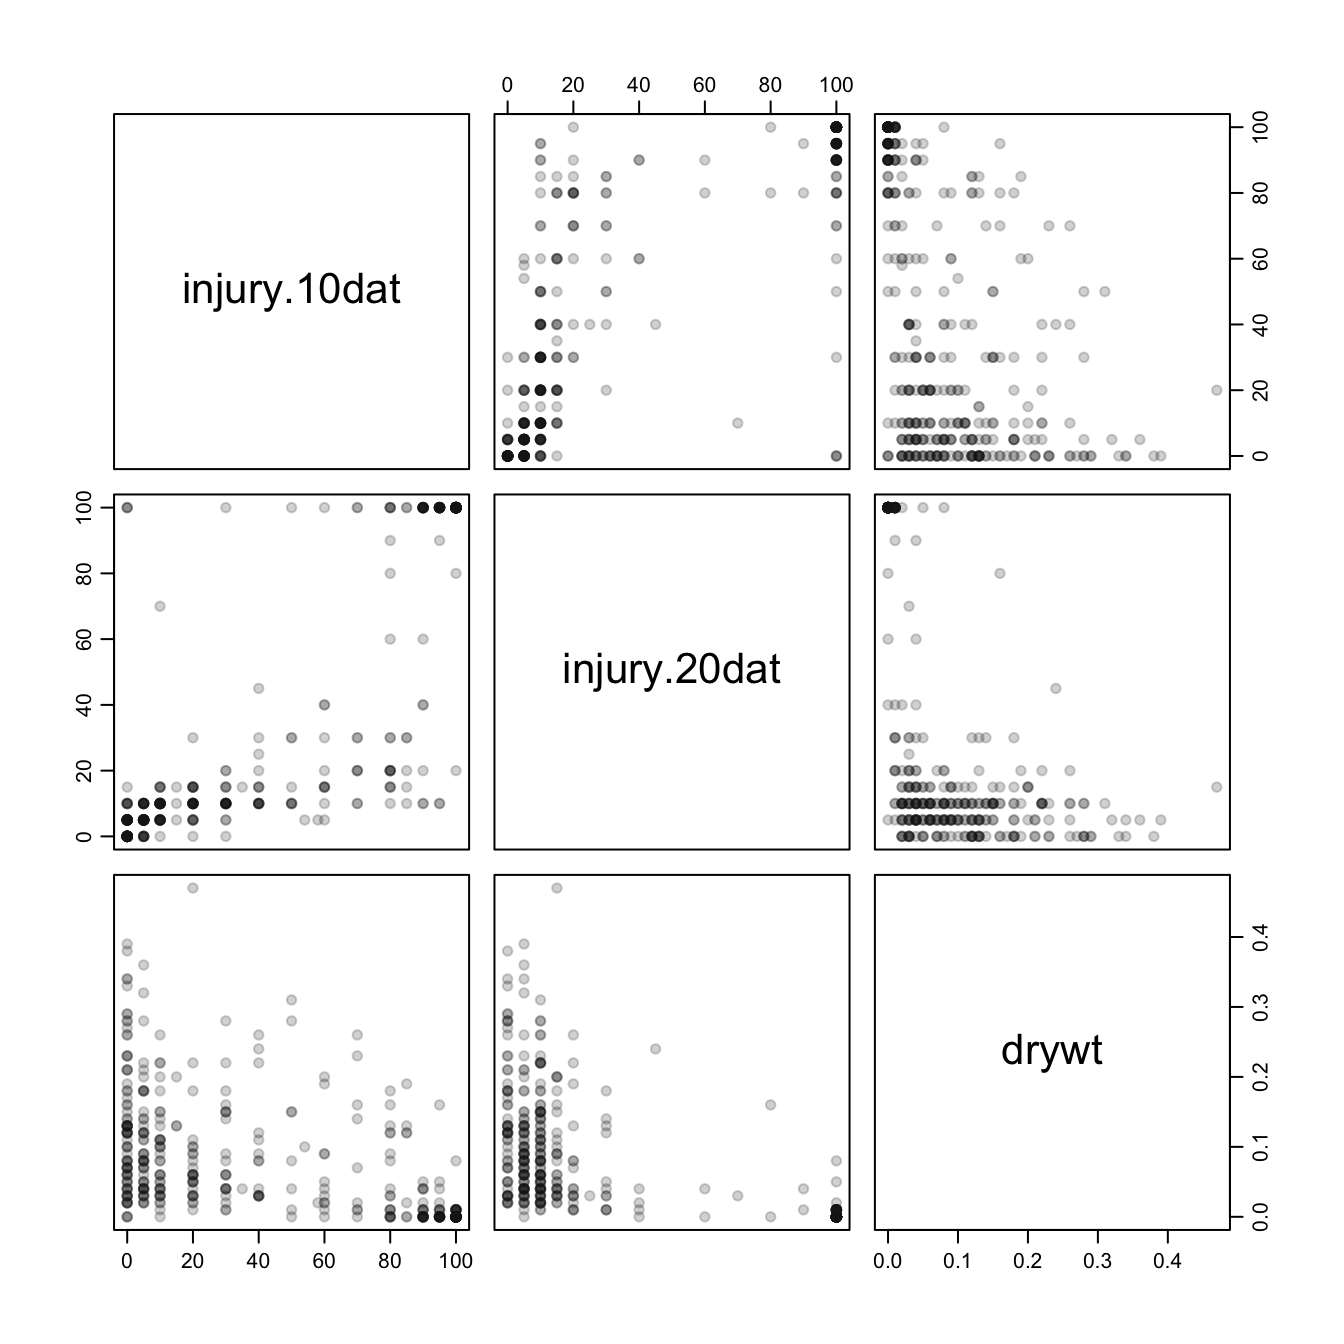
\includegraphics{Rstats4ag_files/figure-latex/figcorrpairs-1.pdf}
\caption{\label{fig:figcorrpairs}\emph{Relationship between injury and dry weight using the \texttt{pairs()} function.}}
\end{figure}

\begin{center}\rule{0.5\linewidth}{0.5pt}\end{center}

\hypertarget{students-t-test}{%
\chapter{Student's t-test}\label{students-t-test}}

\hypertarget{one-sample-t-test}{%
\section{One-sample t-test}\label{one-sample-t-test}}

One of the most basic statistical analyses involves testing whether a group of data is statistically similar to a known value. For example, a researcher may want to know whether the yield data from a wheat experiment was similar to the state-wide average wheat yield for that year. In the example below, yield data (in kg/ha) from 10 different plots is entered manually, and stored in an object named ``yield''. The state-wide dryland wheat average for the same year was 1812 kg/ha. Summary information of the wheat yield, and the differences between the experiment yields and the state average (``yld.diff'') are calculated. The \texttt{t.test()} function is used to calculate the one-sample Student's t-test.

\begin{Shaded}
\begin{Highlighting}[]
\KeywordTok{library}\NormalTok{(tidyverse)}
\NormalTok{yld.dat <-}\StringTok{ }\KeywordTok{data.frame}\NormalTok{(}\DataTypeTok{yield =} \KeywordTok{c}\NormalTok{(}\DecValTok{2280}\NormalTok{, }\DecValTok{2690}\NormalTok{, }\DecValTok{2080}\NormalTok{, }
                                  \DecValTok{2820}\NormalTok{, }\DecValTok{1340}\NormalTok{, }\DecValTok{2080}\NormalTok{, }
                                  \DecValTok{2480}\NormalTok{, }\DecValTok{2420}\NormalTok{, }\DecValTok{2150}\NormalTok{, }\DecValTok{1880}\NormalTok{)) }\OperatorTok
\StringTok{  }\KeywordTok{mutate}\NormalTok{(}\DataTypeTok{yld.diff =}\NormalTok{ yield }\OperatorTok{-}\StringTok{ }\DecValTok{1810}\NormalTok{)}
\NormalTok{yld.dat}
\end{Highlighting}
\end{Shaded}

\begin{verbatim}
##    yield yld.diff
## 1   2280      470
## 2   2690      880
## 3   2080      270
## 4   2820     1010
## 5   1340     -470
## 6   2080      270
## 7   2480      670
## 8   2420      610
## 9   2150      340
## 10  1880       70
\end{verbatim}

\begin{Shaded}
\begin{Highlighting}[]
\KeywordTok{colMeans}\NormalTok{(yld.dat)}
\end{Highlighting}
\end{Shaded}

\begin{verbatim}
##    yield yld.diff 
##     2222      412
\end{verbatim}

The mean wheat yield in the experiment was 2222 kg/ha, 412 kg/ha greater than the state-wide average. There are several possible methods to conduct the one-sample t-test. The first is to subtract the state-wide mean from each observation from the experiment, then test whether the mean difference in yield is different from zero. This is done simply by running the \texttt{t.test()} function on the ``yld.diff'' object calculated above.

\begin{Shaded}
\begin{Highlighting}[]
\KeywordTok{t.test}\NormalTok{(yld.dat}\OperatorTok{$}\NormalTok{yld.diff)}
\end{Highlighting}
\end{Shaded}

\begin{verbatim}
## 
##  One Sample t-test
## 
## data:  yld.dat$yld.diff
## t = 3.065, df = 9, p-value = 0.01346
## alternative hypothesis: true mean is not equal to 0
## 95 percent confidence interval:
##  107.9233 716.0767
## sample estimates:
## mean of x 
##       412
\end{verbatim}

The \texttt{t.test()} output specifies that the alternative hypothesis is that the true mean is not equal to zero, and gives a P-value of 0.013; there is fairly strong evidence that the wheat yield in the experiment is different from the state-wide average. The \texttt{t.test()} function also allows the user to specify a value other than zero to test. This eliminates the need to first calculate the difference of each mean from the state-wide average, and instead, specify the state-wide average within the \texttt{t.test()} function using the \texttt{mu} argument. \texttt{mu} is a common statistical symbol for the population mean.

\begin{Shaded}
\begin{Highlighting}[]
\KeywordTok{t.test}\NormalTok{(yld.dat}\OperatorTok{$}\NormalTok{yield, }\DataTypeTok{mu=}\DecValTok{1810}\NormalTok{)}
\end{Highlighting}
\end{Shaded}

\begin{verbatim}
## 
##  One Sample t-test
## 
## data:  yld.dat$yield
## t = 3.065, df = 9, p-value = 0.01346
## alternative hypothesis: true mean is not equal to 1810
## 95 percent confidence interval:
##  1917.923 2526.077
## sample estimates:
## mean of x 
##      2222
\end{verbatim}

Results are identical to testing whether the difference between experiment yields and the state-wide average yield is different from zero. In both of the above cases, a two-sided alternative hypothesis is tested; that is, the alternate hypothesis being tested is that the experimental average is different from the state-wide average yield. In some cases, though, a one-sided alternative hypothesis would make more practical sense. Perhaps it is assumed \emph{a priori} that the treatments in this experiment will improve wheat yields. Therefore it would be more logical to test whether the wheat yield in the experiment was greater than (not simply different from) the state-wide average. This can be done using the \texttt{alternative} argument in the \texttt{t.test()} function. The \texttt{alternative} argument can be set to either `greater' or `less'.

\begin{Shaded}
\begin{Highlighting}[]
\KeywordTok{t.test}\NormalTok{(yld.dat}\OperatorTok{$}\NormalTok{yield, }\DataTypeTok{alternative=}\StringTok{"greater"}\NormalTok{, }\DataTypeTok{mu=}\DecValTok{1810}\NormalTok{)}
\end{Highlighting}
\end{Shaded}

\begin{verbatim}
## 
##  One Sample t-test
## 
## data:  yld.dat$yield
## t = 3.065, df = 9, p-value = 0.006731
## alternative hypothesis: true mean is greater than 1810
## 95 percent confidence interval:
##  1975.595      Inf
## sample estimates:
## mean of x 
##      2222
\end{verbatim}

As expected, the one-sided alternative produces a p-value of exactly one-half of the two-sided alternative. It appears that there is strong evidence that the experimental mean wheat yield is greater than the state-wide average wheat yield.

\hypertarget{two-sample-t-test}{%
\section{Two-sample t-Test}\label{two-sample-t-test}}

The two-sample t-test is more common than the one-sample test in designed agricultural experiments. In a two-sample t-test, there are two groups (often experimental treatments) on which data is collected. Some examples where the two-sample t-test would be used might include testing isogenic crop varieties to test for yield drag, or comparing two herbicide formulations for absorption or efficacy. Another example from the published literature can be found in \href{http://assbt-jsbr.org/JSBR/Vol47/JSBRVol473and4p127to134CompasisonofConventionalandGlyphosate-ResistanSugarbeettheYarofCommercialInductioninWyoming.pdf}{Kniss et al. (2011)}, where glyphosate-resistant sugarbeet was compared with conventional sugarbeet varieties. For this study, 11 fields in Wyoming were split, with one side planted to glyphosate-resistant varieties, and the other side planted to conventional varieties. The two sides of the field were then managed as the grower thought best for the rest of the year.

\begin{Shaded}
\begin{Highlighting}[]
\NormalTok{sbeet.dat <-}\StringTok{ }\KeywordTok{read.csv}\NormalTok{(}\StringTok{"http://rstats4ag.org/data/sugarbeet.csv"}\NormalTok{) }\OperatorTok
\StringTok{  }\KeywordTok{mutate}\NormalTok{(}\DataTypeTok{Yield =} \KeywordTok{round}\NormalTok{(Yield }\OperatorTok{*}\StringTok{ }\FloatTok{2.24}\NormalTok{, }\DecValTok{1}\NormalTok{)) }\CommentTok{# Convert data to SI units}
\KeywordTok{head}\NormalTok{(sbeet.dat)}
\end{Highlighting}
\end{Shaded}

\begin{verbatim}
##   Field Type Yield
## 1     1    C  72.8
## 2     1    R  74.4
## 3     2    C  64.1
## 4     2    R  65.4
## 5     3    C  56.7
## 6     3    R  68.8
\end{verbatim}

In the ``sugarbeet.csv'' file, each field is represented in two data rows: one row for the glyphosate-resistant (`R') side, and a second row for the conventional side (`C'). Therefore, prior to running the t.test function, the data is divided into two separate data frames using the subset function. The subset function takes the \texttt{sbeet.dat} data frame, and copies only the observations (rows) where the column ``Type'' matches an argument; ''R'' for the first, and ''C'' for the second. This results in one data frame that contains only the glyphosate-resistant observations (``RR'') and one data frame that contains only the conventional observations (``CON'').

\begin{Shaded}
\begin{Highlighting}[]
\NormalTok{RR <-}\StringTok{ }\KeywordTok{subset}\NormalTok{(sbeet.dat, sbeet.dat}\OperatorTok{$}\NormalTok{Type }\OperatorTok{==}\StringTok{ "R"}\NormalTok{)}
\NormalTok{CON <-}\StringTok{ }\KeywordTok{subset}\NormalTok{(sbeet.dat, sbeet.dat}\OperatorTok{$}\NormalTok{Type }\OperatorTok{==}\StringTok{ "C"}\NormalTok{)}
\KeywordTok{t.test}\NormalTok{(RR}\OperatorTok{$}\NormalTok{Yield, CON}\OperatorTok{$}\NormalTok{Yield)}
\end{Highlighting}
\end{Shaded}

\begin{verbatim}
## 
##  Welch Two Sample t-test
## 
## data:  RR$Yield and CON$Yield
## t = 1.3745, df = 19.079, p-value = 0.1852
## alternative hypothesis: true difference in means is not equal to 0
## 95 percent confidence interval:
##  -4.064981 19.628617
## sample estimates:
## mean of x mean of y 
##  58.60909  50.82727
\end{verbatim}

The t.test function then compares the ``Yield'' column from the RR data frame to yield data in the the CON data frame. The t-test output provides the mean yield for each group (58.6 tons/ha for glyphosate-resistant, and 50.8 tons/ha for the conventional). In this case it appears that due to the variability in the data, there is not strong evidence for a difference between the two systems (P=0.185). Since there are only two groups in the ``Type'' column, we can simplify the code above by not subsetting the data ahead of time. We can simply use the \texttt{t.test()} function and specify that Type contains the relevant treatment information by using the formula \texttt{response\ \textasciitilde{}\ groups}, specifically in this case: \texttt{Yield\ \textasciitilde{}\ Type}.

\begin{Shaded}
\begin{Highlighting}[]
\KeywordTok{t.test}\NormalTok{(Yield }\OperatorTok{~}\StringTok{ }\NormalTok{Type, }\DataTypeTok{data=}\NormalTok{sbeet.dat)}
\end{Highlighting}
\end{Shaded}

\hypertarget{paired-t-test}{%
\section{Paired t-Test}\label{paired-t-test}}

A special case of the two-sample t-test is the paired t-test. In this sugarbeet example, the two-sample t-test assumes the 11 observations on the glyphosate-resistant fields are independent from the 11 observations on the conventional fields. In reality, this was not the case. The way the study was carried out, conventional sugarbeet varieties were planted in the same (or immediately adjacent) field as the glyphosate-resistant varieties. Therefore, the glyphosate-resistant observation was not actually independent from the observation on the conventional side of the field. For each field, weather, irrigation, fertility, etc. were all the same for both sides of the field. We can therefore assume that most of the variability between the conventional and glyphosate-resistant portions of the first field is due to the varieties, or the way each side of the field was managed (herbicides, tillage, etc.), and not due to unrelated external factors. Because the purpose of the study was to compare the glyphosate-resistant and conventional systems, it is more desirable to consider the two sides of the same field as ``paired'' samples, to which different treatments were applied. This can be achieved by adding the argument \texttt{paired=T} to the \texttt{t.test()} function.

\begin{Shaded}
\begin{Highlighting}[]
\KeywordTok{t.test}\NormalTok{(Yield }\OperatorTok{~}\StringTok{ }\NormalTok{Type, }\DataTypeTok{data=}\NormalTok{sbeet.dat, }\DataTypeTok{paired=}\NormalTok{T)}
\end{Highlighting}
\end{Shaded}

\begin{verbatim}
## 
##  Paired t-test
## 
## data:  Yield by Type
## t = -3.3302, df = 10, p-value = 0.007615
## alternative hypothesis: true difference in means is not equal to 0
## 95 percent confidence interval:
##  -12.988388  -2.575248
## sample estimates:
## mean of the differences 
##               -7.781818
\end{verbatim}

In this case, we reach a very different conclusion; that within a field pair, there is very strong evidence that the difference between group means is different from zero (P=0.008); or that within each field, yield in the glyphosate-resistant system was different from conventional sugarbeet yields. On average, the glyphosate-resistant system resulted in 7.8 tons/ha greater yield than the conventional system. Notice that the paired t-test provides the exact same result as if we subtract the conventional yields from the glyphosate-resistant yields for each pair, then conduct a one-sample t-test on the difference.

\begin{Shaded}
\begin{Highlighting}[]
\NormalTok{RR}\OperatorTok{$}\NormalTok{Yield }\OperatorTok{-}\StringTok{ }\NormalTok{CON}\OperatorTok{$}\NormalTok{Yield ->}\StringTok{ }\NormalTok{diff.Yield}
\KeywordTok{t.test}\NormalTok{(diff.Yield)}
\end{Highlighting}
\end{Shaded}

In this example, there was no \emph{a priori} expectation that the glyphosate-resistant system would yield more or less than the conventional system, and therefore the two-sided alternative hypothesis is appropriate.

\begin{center}\rule{0.5\linewidth}{0.5pt}\end{center}

\hypertarget{anova}{%
\chapter{Analysis of Variance (ANOVA)}\label{anova}}

\hypertarget{one-way-analysis-of-variance}{%
\section{One-Way Analysis of Variance}\label{one-way-analysis-of-variance}}

Some of the most often used experimental designs in weed science include completely randomized designs (CRD) and randomized complete block designs (RCBD). These experiments are typically analyzed using analysis of variance (ANOVA). The one-way ANOVA is used to determine the effect of a single factor (with at least three levels) on a response variable. Where only two levels of a single factor are of interest, the \texttt{t.test()} function will be more appropriate. There are several ways to conduct an ANOVA in the base R package. The \texttt{aov()} function requires a response variable and the explanatory variable separated with the \texttt{\textasciitilde{}} symbol. It is important when using the \texttt{aov()} function that your data are balanced, with no missing values. For data sets with missing values or unbalanced designs, please see the section on mixed effects models.

The ``FlumiBeans'' data set is from a herbicide trial conducted in Wyoming during three different years (2009 through 2011). Five different herbicide treatments were applied, plus nontreated and handweeded controls for a total of seven treatments. The study was a randomized complete block design (RCBD) each year. There were 3 replicates in 2009, but 4 replicates in subsequent years. The response variable in this data set is dry bean (\emph{Phaseolus vulgaris}) density 4 weeks after planting expressend in plants per acre.

It is important to note that some of our factor variables have been expressed in the .csv file as numbers (e.g. `year' and `block'), and consequently, R will recognized these factors as numeric variables. It is important for our ANOVA that these variables be included as factors, and not as numeric variables. We can use the \texttt{dplyr} package from the \texttt{tidyverse} to convert these variables to the proper form as we read them with the \texttt{mutate()} function.

\begin{Shaded}
\begin{Highlighting}[]
\KeywordTok{library}\NormalTok{(tidyverse)}

\NormalTok{bean.dat <-}\StringTok{ }\KeywordTok{read.csv}\NormalTok{(}\StringTok{"http://rstats4ag.org/data/FlumiBeans.csv"}\NormalTok{) }\OperatorTok
\StringTok{  }\KeywordTok{mutate}\NormalTok{(}\DataTypeTok{population.4wk =}\NormalTok{ population}\FloatTok{.4}\NormalTok{wk }\OperatorTok{*}\StringTok{ }\FloatTok{2.47}\NormalTok{, }\CommentTok{# Convert to SI units}
         \DataTypeTok{year =} \KeywordTok{factor}\NormalTok{(year),}
         \DataTypeTok{block =} \KeywordTok{factor}\NormalTok{(block),}
         \DataTypeTok{treatment =} \KeywordTok{factor}\NormalTok{(treatment))}
\KeywordTok{glimpse}\NormalTok{(bean.dat)}
\end{Highlighting}
\end{Shaded}

\begin{verbatim}
## Rows: 77
## Columns: 4
## $ year           <fct> 2009, 2009, 2009, 2009, 2009, 2009, 2009, 2009, 2009, 2009, 2009, 2009, ...
## $ treatment      <fct> Nontreated, Nontreated, Nontreated, flumioxazin + trifluralin, flumioxaz...
## $ block          <fct> 1, 2, 3, 1, 2, 3, 1, 2, 3, 1, 2, 3, 1, 2, 3, 1, 2, 3, 1, 2, 3, 1, 2, 3, ...
## $ population.4wk <dbl> 137719.79, 111895.94, 94682.51, 34429.33, 68858.66, 77466.61, 25821.38, ...
\end{verbatim}

For this analysis, we want to look at a One-Way analysis of variance, and so we will focus on the data from only one year. We can subset the data to include only this year using the \texttt{filter()} function from the \texttt{dplyr} package, and call this subsetted data \texttt{bean.09}.

\begin{Shaded}
\begin{Highlighting}[]
\NormalTok{bean}\FloatTok{.09}\NormalTok{ <-}\StringTok{ }\NormalTok{bean.dat }\OperatorTok
\StringTok{  }\KeywordTok{filter}\NormalTok{(year }\OperatorTok{==}\StringTok{ }\DecValTok{2009}\NormalTok{)}
\end{Highlighting}
\end{Shaded}

We will then use the \texttt{aov()} function to generate the One-way ANOVA to see if herbicide treatment had an effect on dry bean population (expressed in plants per hectare) in 2009.

\begin{Shaded}
\begin{Highlighting}[]
\KeywordTok{aov}\NormalTok{(population}\FloatTok{.4}\NormalTok{wk }\OperatorTok{~}\StringTok{ }\NormalTok{block}\OperatorTok{+}\NormalTok{treatment, }\DataTypeTok{data=}\NormalTok{bean}\FloatTok{.09}\NormalTok{)->b09.aov}
\end{Highlighting}
\end{Shaded}

\hypertarget{checking-anova-assumptions}{%
\subsection{Checking ANOVA assumptions}\label{checking-anova-assumptions}}

ANOVA assumes (1) errors are normally distributed, (2) variances are homogeneous, and (3) observations are independent of each other. ANOVA is fairly robust to violations of the normality assumption, and thus it typically requires a rather severe violation before remedial measures are warranted. However, it is still wise to check the normality assumption prior to interpreting the ANOVA results. Three methods are provided to check normality of the response variable of interest: the Shapiro-Wilks test, a stem and leaf plot, and a Normal Q-Q plot. The model residuals are automatically stored within the ANOVA model produced with the \texttt{aov()} function, and thus we can call upon the model to view and test the residuals for normality. We can get the residuals by using the \texttt{resid()} function, or by appending \texttt{\$resid} onto the model fit. \texttt{resid(b09.aov)} and \texttt{b09.aov\$resid} will provide the same result.

\begin{Shaded}
\begin{Highlighting}[]
\KeywordTok{shapiro.test}\NormalTok{(b09.aov}\OperatorTok{$}\NormalTok{resid)}
\end{Highlighting}
\end{Shaded}

\begin{verbatim}
## 
##  Shapiro-Wilk normality test
## 
## data:  b09.aov$resid
## W = 0.9718, p-value = 0.7726
\end{verbatim}

\begin{Shaded}
\begin{Highlighting}[]
\KeywordTok{stem}\NormalTok{(b09.aov}\OperatorTok{$}\NormalTok{resid)}
\end{Highlighting}
\end{Shaded}

\begin{verbatim}
## 
##   The decimal point is 4 digit(s) to the right of the |
## 
##   -2 | 690
##   -0 | 88607431
##    0 | 222599
##    2 | 2787
\end{verbatim}



\begin{Shaded}
\begin{Highlighting}[]
\KeywordTok{par}\NormalTok{(}\DataTypeTok{mar=}\KeywordTok{c}\NormalTok{(}\FloatTok{3.2}\NormalTok{,}\FloatTok{3.2}\NormalTok{,}\DecValTok{2}\NormalTok{,}\FloatTok{0.5}\NormalTok{), }\DataTypeTok{mgp=}\KeywordTok{c}\NormalTok{(}\DecValTok{2}\NormalTok{,.}\DecValTok{7}\NormalTok{,}\DecValTok{0}\NormalTok{))}
\KeywordTok{qqnorm}\NormalTok{(b09.aov}\OperatorTok{$}\NormalTok{resid)}
\KeywordTok{qqline}\NormalTok{(b09.aov}\OperatorTok{$}\NormalTok{resid)}
\end{Highlighting}
\end{Shaded}

\begin{figure}
\centering
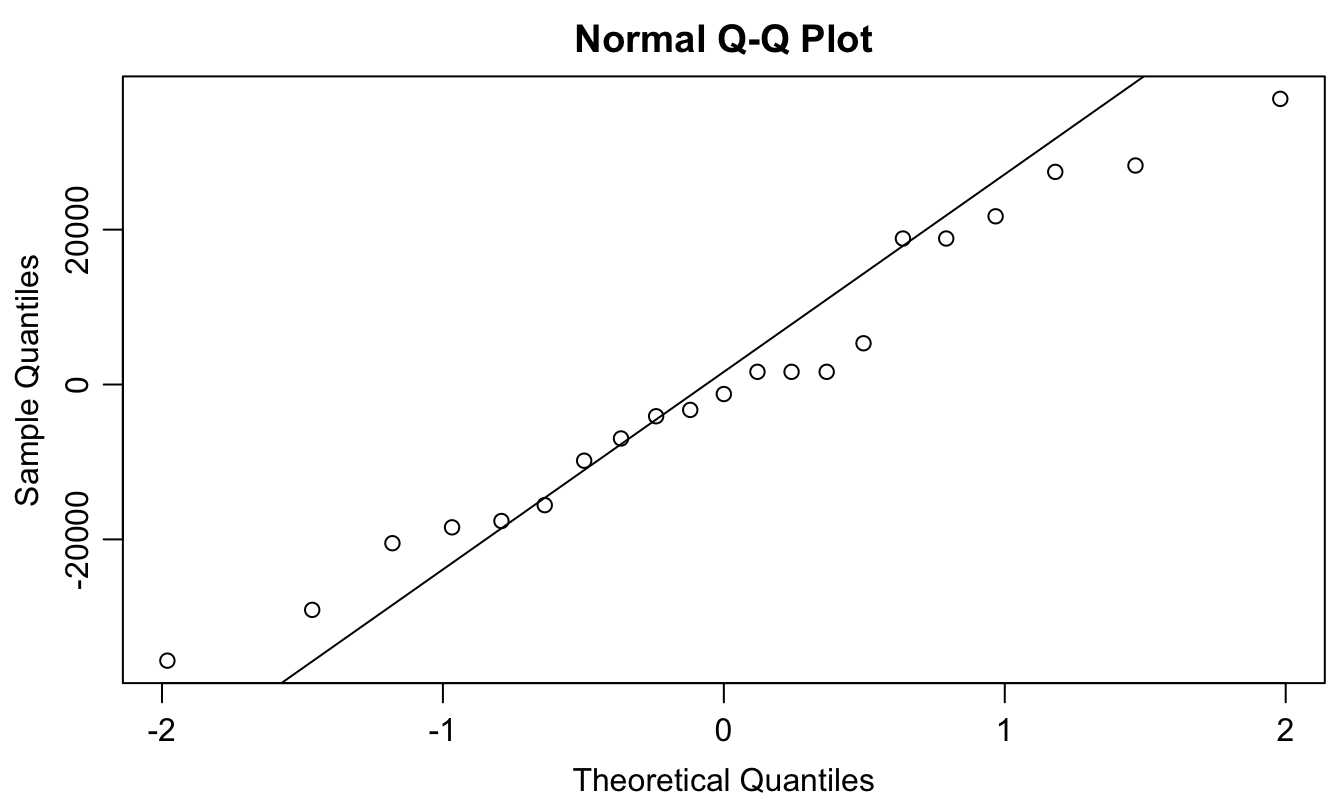
\includegraphics{Rstats4ag_files/figure-latex/fignormalqq-1.pdf}
\caption{\label{fig:fignormalqq}\emph{Normal Q-Q plot to check the assumption of normal distribution of residuals.}}
\end{figure}

It appears that the residuals in this case are at least close to normally distributed. The most common next step if residuals are not normally distributed would be to attempt a transformation. However, it is worth noting that there are other, more \href{https://dl.sciencesocieties.org/publications/aj/articles/107/2/811}{modern methods to deal with non-normality that should be strongly considered}.

The next assumption to test is homogeneity of variance. Formal tests for homogeneity of variance include the Bartlett (parametric) and Fligner-Killeen (non-parametric) tests. These tests can be used in conjunction with box plots to determine the level of heterogeneity of variance between treatments.

\begin{Shaded}
\begin{Highlighting}[]
\KeywordTok{bartlett.test}\NormalTok{(bean}\FloatTok{.09}\OperatorTok{$}\NormalTok{population}\FloatTok{.4}\NormalTok{wk, bean}\FloatTok{.09}\OperatorTok{$}\NormalTok{treatment)}
\end{Highlighting}
\end{Shaded}

\begin{verbatim}
## 
##  Bartlett test of homogeneity of variances
## 
## data:  bean.09$population.4wk and bean.09$treatment
## Bartlett's K-squared = 3.7865, df = 6, p-value = 0.7055
\end{verbatim}

\begin{Shaded}
\begin{Highlighting}[]
\KeywordTok{fligner.test}\NormalTok{(bean}\FloatTok{.09}\OperatorTok{$}\NormalTok{population}\FloatTok{.4}\NormalTok{wk, bean}\FloatTok{.09}\OperatorTok{$}\NormalTok{treatment)}
\end{Highlighting}
\end{Shaded}

\begin{verbatim}
## 
##  Fligner-Killeen test of homogeneity of variances
## 
## data:  bean.09$population.4wk and bean.09$treatment
## Fligner-Killeen:med chi-squared = 3.2494, df = 6, p-value = 0.777
\end{verbatim}

Formal tests do not indicate a problem (p\textgreater{}0.7), and box plots (Figure \ref{fig:figbeanboxplots}) indicate that things are reasonable similar. Perhaps the handweeded and EPTC + ethalfluralin treatments have less variability than the others, but differences are not too dramatic, especially considering there were only 3 replicates per treatment in 2009.



\begin{Shaded}
\begin{Highlighting}[]
\KeywordTok{par}\NormalTok{(}\DataTypeTok{mar=}\KeywordTok{c}\NormalTok{(}\FloatTok{4.2}\NormalTok{,}\DecValTok{12}\NormalTok{,}\FloatTok{0.5}\NormalTok{,}\FloatTok{1.5}\NormalTok{), }\DataTypeTok{mgp=}\KeywordTok{c}\NormalTok{(}\DecValTok{2}\NormalTok{,.}\DecValTok{7}\NormalTok{,}\DecValTok{0}\NormalTok{))}
\KeywordTok{boxplot}\NormalTok{(bean}\FloatTok{.09}\OperatorTok{$}\NormalTok{population}\FloatTok{.4}\NormalTok{wk}\OperatorTok{/}\DecValTok{1000} \OperatorTok{~}\StringTok{ }\NormalTok{bean}\FloatTok{.09}\OperatorTok{$}\NormalTok{treatment, }\DataTypeTok{horizontal=}\NormalTok{T, }
        \DataTypeTok{las=}\DecValTok{1}\NormalTok{, }\DataTypeTok{xlab=}\StringTok{"Bean plants per hectare (thousands)"}\NormalTok{,}
        \DataTypeTok{ylab=}\StringTok{""}\NormalTok{)}
\end{Highlighting}
\end{Shaded}

\begin{figure}
\centering
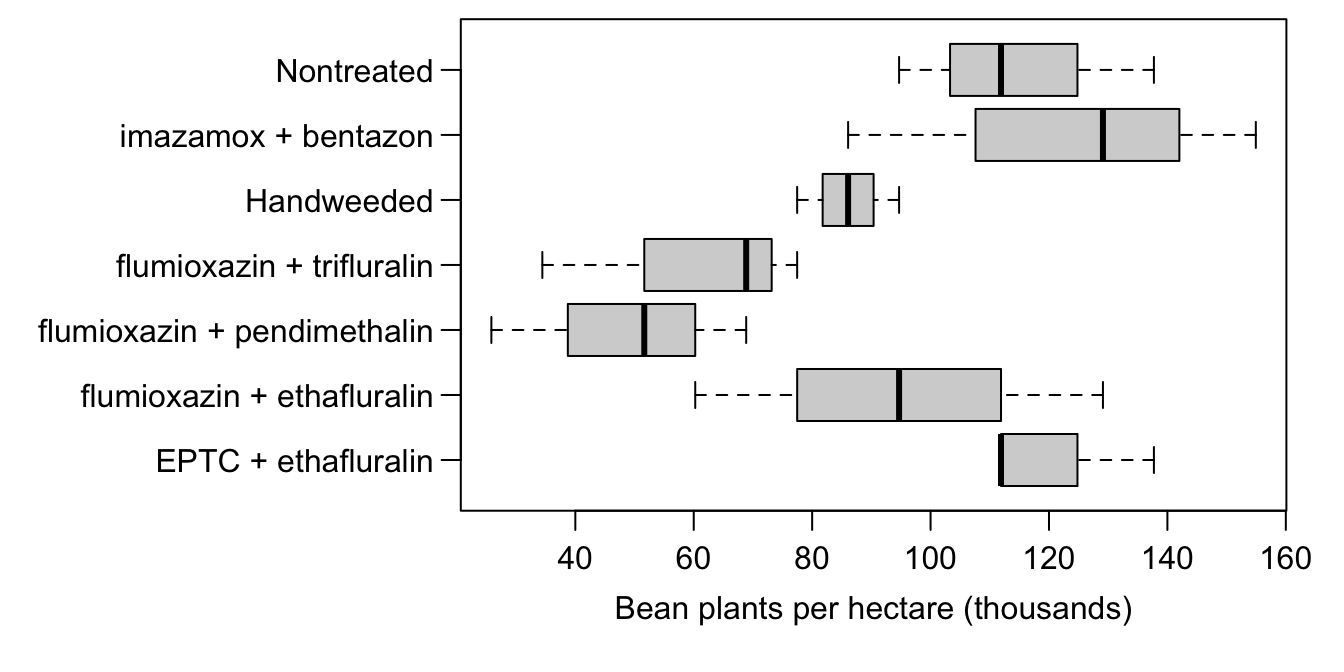
\includegraphics{Rstats4ag_files/figure-latex/figbeanboxplots-1.pdf}
\caption{\label{fig:figbeanboxplots}\emph{Boxplots showing the effect of weed control treatment on dry edible bean plants per hectare.}}
\end{figure}

Simply plotting the aov fit in R {[}e.g.~Figure \ref{fig:figanovadiagnostics}{]} will provide a series of diagnostic plots as well. The first two plots are the residuals vs fitted values, and the Normal Q-Q plot, which can be plotted at the same time with the following code:



\begin{Shaded}
\begin{Highlighting}[]
\KeywordTok{par}\NormalTok{(}\DataTypeTok{mar=}\KeywordTok{c}\NormalTok{(}\FloatTok{4.2}\NormalTok{,}\FloatTok{4.2}\NormalTok{,}\FloatTok{2.2}\NormalTok{,}\DecValTok{1}\NormalTok{), }\DataTypeTok{mfrow=}\KeywordTok{c}\NormalTok{(}\DecValTok{1}\NormalTok{,}\DecValTok{2}\NormalTok{), }\DataTypeTok{mgp=}\KeywordTok{c}\NormalTok{(}\DecValTok{2}\NormalTok{,.}\DecValTok{7}\NormalTok{,}\DecValTok{0}\NormalTok{))}
\KeywordTok{plot}\NormalTok{(b09.aov, }\DataTypeTok{which=}\DecValTok{1}\OperatorTok{:}\DecValTok{2}\NormalTok{)}
\end{Highlighting}
\end{Shaded}

\begin{figure}
\centering
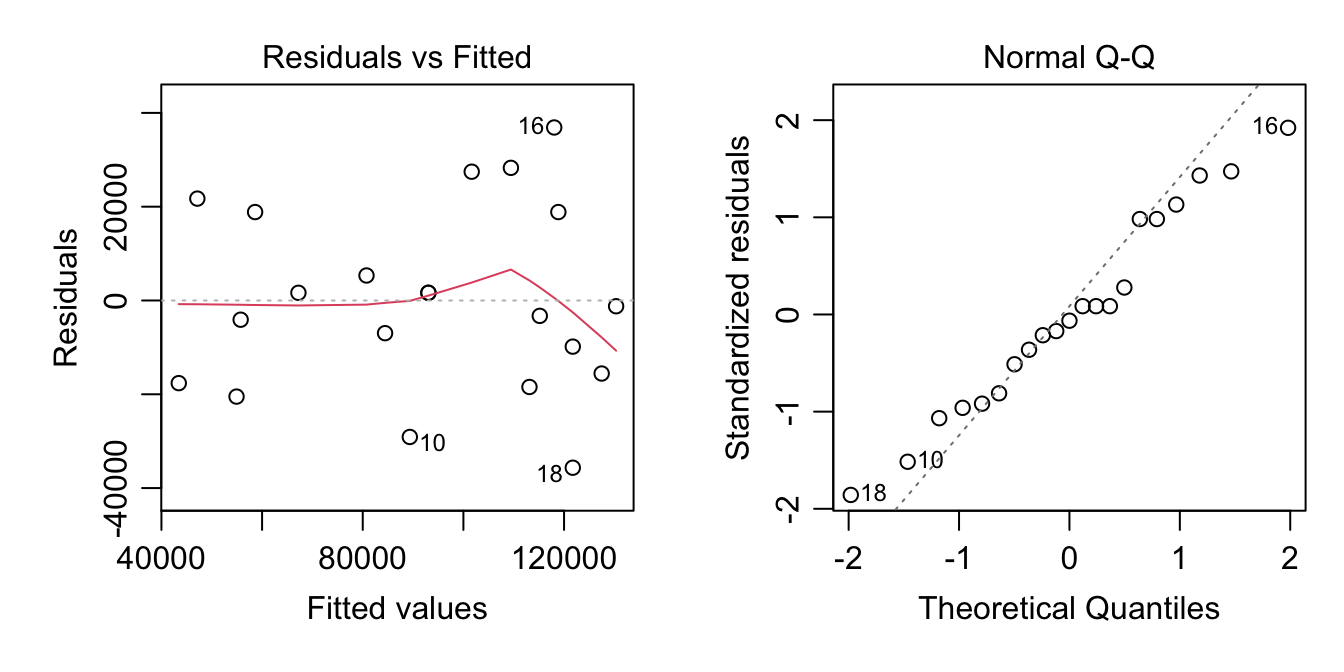
\includegraphics{Rstats4ag_files/figure-latex/figanovadiagnostics-1.pdf}
\caption{\label{fig:figanovadiagnostics}\emph{Model diagnostic plots for the dry edible bean ANOVA model.}}
\end{figure}

Since neither the normality nor homogeneity of variance assumptions were dramatically violated, and ANOVA is fairly robust to violations of these assumptions, it seems safe to proceed with interpretation of the ANOVA results. The third assumption (independence of observations) is not something we will test statistically; it is up to the researcher to ensure that they are collecting data in a way that does not violate this assumption.

Finally, after the assumptions have been checked, and remedial measures taken if necessary, we will want to know whether there is a significant effect of herbicide treatment on dry bean population density. Once again, we can use the \texttt{summary()} function along with the stored model to obtain this information. The resulting ANOVA table indicates that we have pretty strong evidence that there are differences in dry bean plants per acre due to herbicide treatment (p = 0.019).

\begin{Shaded}
\begin{Highlighting}[]
\KeywordTok{summary}\NormalTok{(b09.aov)}
\end{Highlighting}
\end{Shaded}

\begin{verbatim}
##             Df    Sum Sq   Mean Sq F value Pr(>F)  
## block        2 5.574e+08 2.787e+08   0.432 0.6589  
## treatment    6 1.569e+10 2.615e+09   4.055 0.0188 *
## Residuals   12 7.740e+09 6.450e+08                 
## ---
## Signif. codes:  0 '***' 0.001 '**' 0.01 '*' 0.05 '.' 0.1 ' ' 1
\end{verbatim}

\hypertarget{mean-separation---agricolae-package}{%
\subsection{Mean Separation - agricolae package}\label{mean-separation---agricolae-package}}

The \texttt{agricolae} package has several functions for mean separation, including the \texttt{LSD.test()} function that will compare means using Fisher's LSD. The LSD.test computes a lot of useful information that can be extracted for later use. You can use the \texttt{str(bean.lsd)} function to learn more about what is available. Below, we will look at the \texttt{\$group} section which gives the treatment means and mean separation, and the \texttt{\$statistics} section which provides the LSD value (among other things).

\begin{Shaded}
\begin{Highlighting}[]
\KeywordTok{library}\NormalTok{(agricolae)}
\NormalTok{bean.lsd <-}\StringTok{ }\KeywordTok{LSD.test}\NormalTok{(b09.aov, }\DataTypeTok{trt=}\StringTok{"treatment"}\NormalTok{)}
\NormalTok{bean.lsd}\OperatorTok{$}\NormalTok{group}
\end{Highlighting}
\end{Shaded}

\begin{verbatim}
##                             population.4wk groups
## imazamox + bentazon              123373.21      a
## EPTC + ethafluralin              120503.89      a
## Nontreated                       114766.08      a
## flumioxazin + ethafluralin        94682.51     ab
## Handweeded                        86074.56    abc
## flumioxazin + trifluralin         60251.53     bc
## flumioxazin + pendimethalin       48775.09      c
\end{verbatim}

\begin{Shaded}
\begin{Highlighting}[]
\NormalTok{bean.lsd}\OperatorTok{$}\NormalTok{statistics}
\end{Highlighting}
\end{Shaded}

\begin{verbatim}
##     MSerror Df     Mean       CV  t.value      LSD
##   645034519 12 92632.41 27.41754 2.178813 45182.03
\end{verbatim}

To get standard deviations and confidence limits, we could type \texttt{bean.lsd\$means}. The \texttt{agricolae} package can also calculate Tukey's HSD using the \texttt{HSD.test()} function. The syntax above is the same, simply changing \texttt{LSD.test} to \texttt{HSD.test}.

\hypertarget{mean-separation---emmeans-and-multcomp-packages}{%
\subsection{Mean Separation - emmeans and multcomp packages}\label{mean-separation---emmeans-and-multcomp-packages}}

The \texttt{emmeans} and \texttt{multcomp} packages are also useful for separating means, and has the advantage that it can be used for linear, nonlinear, and mixed effects models.

\begin{Shaded}
\begin{Highlighting}[]
\KeywordTok{library}\NormalTok{(emmeans)}
\KeywordTok{library}\NormalTok{(multcomp)}
\NormalTok{b09.emm <-}\StringTok{ }\KeywordTok{emmeans}\NormalTok{(b09.aov, }\OperatorTok{~}\StringTok{ }\NormalTok{treatment)}
\KeywordTok{pairs}\NormalTok{(b09.emm) }\CommentTok{# prints out all Tukey-adjusted pairwise comparisons}
\NormalTok{multcomp}\OperatorTok{::}\KeywordTok{cld}\NormalTok{(b09.emm, }\DataTypeTok{Letters=}\NormalTok{LETTERS) }\CommentTok{# corresponding compact letter display (cld)}
\KeywordTok{pairs}\NormalTok{(b09.emm, }\DataTypeTok{adjust=}\StringTok{"none"}\NormalTok{) }\CommentTok{# prints out all unadjusted pairwise comparisons}
\NormalTok{multcomp}\OperatorTok{::}\KeywordTok{cld}\NormalTok{(b09.emm, }\DataTypeTok{Letters=}\NormalTok{LETTERS, }\DataTypeTok{adjust=}\StringTok{"none"}\NormalTok{) }\CommentTok{# corresponding compact letter display (cld)}
\end{Highlighting}
\end{Shaded}

\hypertarget{multi-factor-anova}{%
\section{Multi-Factor ANOVA}\label{multi-factor-anova}}

We'll now look at the second and third year of the study, beginning by subsetting the data to include only these years.

\begin{Shaded}
\begin{Highlighting}[]
\NormalTok{bean2.dat <-}\StringTok{ }\NormalTok{bean.dat }\OperatorTok
\StringTok{  }\KeywordTok{filter}\NormalTok{(year}\OperatorTok{==}\DecValTok{2010} \OperatorTok{|}\StringTok{ }\NormalTok{year}\OperatorTok{==}\DecValTok{2011}\NormalTok{)}
\KeywordTok{summary}\NormalTok{(bean2.dat)}
\end{Highlighting}
\end{Shaded}

\begin{verbatim}
##    year                          treatment block  population.4wk  
##  2009: 0   EPTC + ethafluralin        :8   1:14   Min.   : 17216  
##  2010:28   flumioxazin + ethafluralin :8   2:14   1st Qu.: 51645  
##  2011:28   flumioxazin + pendimethalin:8   3:14   Median : 95761  
##            flumioxazin + trifluralin  :8   4:14   Mean   : 86038  
##            Handweeded                 :8          3rd Qu.:115665  
##            imazamox + bentazon        :8          Max.   :163541  
##            Nontreated                 :8
\end{verbatim}

We'll now incorporate year as a fixed effect in the analysis. We're going to exclude the 2009 data because it does not have the same number of replicates as the other two years of data. The \texttt{aov()} function is not appropriate for unbalanced data. We will look at how to best handle this in a later section using mixed effects. We're also going to incorporate the blocking design into the model using the \texttt{Error()} argument. Blocking was used in each year of the field study (in a randomized complete block design). Because the trial was located in a different field each year, there is no reason to think that block 1 would result in a similar impact from one year to the next. Therefore, the effect of block is nested within year. We can specify this structure in the \texttt{aov()} function by using the \texttt{/} operator.

\begin{Shaded}
\begin{Highlighting}[]
\NormalTok{bean2.aov<-}\KeywordTok{aov}\NormalTok{(population}\FloatTok{.4}\NormalTok{wk }\OperatorTok{~}\StringTok{ }\NormalTok{year}\OperatorTok{*}\NormalTok{treatment }\OperatorTok{+}\StringTok{ }\KeywordTok{Error}\NormalTok{(year}\OperatorTok{/}\NormalTok{block), }
               \DataTypeTok{data=}\NormalTok{bean2.dat)}
\KeywordTok{summary}\NormalTok{(bean2.aov)}
\end{Highlighting}
\end{Shaded}

\begin{verbatim}
## 
## Error: year
##      Df   Sum Sq  Mean Sq
## year  1 5.46e+09 5.46e+09
## 
## Error: year:block
##           Df    Sum Sq   Mean Sq F value Pr(>F)
## Residuals  6 1.363e+09 227216916               
## 
## Error: Within
##                Df    Sum Sq   Mean Sq F value   Pr(>F)    
## treatment       6 6.588e+10 1.098e+10  51.925 2.91e-16 ***
## year:treatment  6 5.422e+09 9.036e+08   4.273  0.00238 ** 
## Residuals      36 7.612e+09 2.114e+08                     
## ---
## Signif. codes:  0 '***' 0.001 '**' 0.01 '*' 0.05 '.' 0.1 ' ' 1
\end{verbatim}

Adding the Error term into the model results in 3 separate sections of the ANOVA table, corresponding to the three separate error terms: year, year:block, and within. In this case no F or P-values are calculated for the year effect. We could do that manually by dividing the Mean Square for year by the Mean Square for year:block, but it is clear just by looking at the numbers that the F value will be quite high (greater than 23, in fact). However, if we want \texttt{aov()} to calculate the P-value for us, we can specify the year*block error term by creating a new variable that contains the combined information. We will do this below using the \texttt{with()} function.

\begin{Shaded}
\begin{Highlighting}[]
\NormalTok{bean2.dat}\OperatorTok{$}\NormalTok{yrblock  <-}\StringTok{ }\KeywordTok{with}\NormalTok{(bean2.dat, }\KeywordTok{factor}\NormalTok{(year)}\OperatorTok{:}\KeywordTok{factor}\NormalTok{(block))}
\NormalTok{bean2.aov2<-}\KeywordTok{aov}\NormalTok{(population}\FloatTok{.4}\NormalTok{wk }\OperatorTok{~}\StringTok{ }\NormalTok{year}\OperatorTok{*}\NormalTok{treatment }\OperatorTok{+}\StringTok{ }\KeywordTok{Error}\NormalTok{(yrblock), }
                \DataTypeTok{data=}\NormalTok{bean2.dat)}
\KeywordTok{summary}\NormalTok{(bean2.aov2)}
\end{Highlighting}
\end{Shaded}

\begin{verbatim}
## 
## Error: yrblock
##           Df    Sum Sq   Mean Sq F value  Pr(>F)   
## year       1 5.460e+09 5.460e+09   24.03 0.00271 **
## Residuals  6 1.363e+09 2.272e+08                   
## ---
## Signif. codes:  0 '***' 0.001 '**' 0.01 '*' 0.05 '.' 0.1 ' ' 1
## 
## Error: Within
##                Df    Sum Sq   Mean Sq F value   Pr(>F)    
## treatment       6 6.588e+10 1.098e+10  51.925 2.91e-16 ***
## year:treatment  6 5.422e+09 9.036e+08   4.273  0.00238 ** 
## Residuals      36 7.612e+09 2.114e+08                     
## ---
## Signif. codes:  0 '***' 0.001 '**' 0.01 '*' 0.05 '.' 0.1 ' ' 1
\end{verbatim}

The Mean Square for year and the year:block interaction are the same as before, as expected, but now the F and P-values are provided. However, this is not as important in this case, as there is a significant year by treatment interaction effect, making the main effect of year less interesting.

\hypertarget{mean-separation}{%
\subsection{Mean Separation}\label{mean-separation}}

Due to the different error terms, getting mean separation from the \texttt{LSD.test()} function in this case is not as straightforward as with only one factor. It can still be done by specifying the response, treatment, error degrees of freedom, and mean square error manually.

\begin{Shaded}
\begin{Highlighting}[]
\NormalTok{bean2.lsd<-}\KeywordTok{LSD.test}\NormalTok{(bean2.dat}\OperatorTok{$}\NormalTok{population}\FloatTok{.4}\NormalTok{wk,}
                    \KeywordTok{with}\NormalTok{(bean2.dat, year}\OperatorTok{:}\NormalTok{treatment), }
                    \DecValTok{36}\NormalTok{, }\FloatTok{2.11e+08}\NormalTok{)}
\NormalTok{bean2.lsd}\OperatorTok{$}\NormalTok{groups}
\end{Highlighting}
\end{Shaded}

\begin{verbatim}
##                                  bean2.dat$population.4wk groups
## 2010:imazamox + bentazon                        142023.15      a
## 2010:EPTC + ethafluralin                        139871.16      a
## 2010:Handweeded                                 124807.87     ab
## 2010:Nontreated                                 124807.87     ab
## 2011:Handweeded                                 104369.23     bc
## 2011:Nontreated                                  97375.43      c
## 2011:imazamox + bentazon                         95761.28      c
## 2011:EPTC + ethafluralin                         94147.76      c
## 2011:flumioxazin + trifluralin                   57026.74      d
## 2010:flumioxazin + trifluralin                   51644.61     de
## 2010:flumioxazin + pendimethalin                 49493.24     de
## 2011:flumioxazin + pendimethalin                 48956.64     de
## 2010:flumioxazin + ethafluralin                  38733.92     de
## 2011:flumioxazin + ethafluralin                  35506.87      e
\end{verbatim}

Alternatively, we can use the \texttt{emmeans} package, to get the confidence intervals and pairwise comparisons.

\begin{Shaded}
\begin{Highlighting}[]
\KeywordTok{emmeans}\NormalTok{(bean2.aov2, }\DataTypeTok{specs =}\NormalTok{ pairwise }\OperatorTok{~}\StringTok{ }\NormalTok{year}\OperatorTok{:}\NormalTok{treatment)}
\end{Highlighting}
\end{Shaded}

It seems there is general trend for treatments containing flumioxazin to have fewer bean plants. But having the different years mixed together makes it difficult to see, so an alternative approach would be to simply calculate the means using \texttt{tapply()} and print out the LSD value.

\begin{Shaded}
\begin{Highlighting}[]
\KeywordTok{round}\NormalTok{(}\KeywordTok{tapply}\NormalTok{(bean2.dat}\OperatorTok{$}\NormalTok{population}\FloatTok{.4}\NormalTok{wk, }
             \KeywordTok{list}\NormalTok{(bean2.dat}\OperatorTok{$}\NormalTok{treatment, bean2.dat}\OperatorTok{$}\NormalTok{year), mean), }\DecValTok{-3}\NormalTok{)}
\end{Highlighting}
\end{Shaded}

\begin{verbatim}
##                             2009   2010   2011
## EPTC + ethafluralin           NA 140000  94000
## flumioxazin + ethafluralin    NA  39000  36000
## flumioxazin + pendimethalin   NA  49000  49000
## flumioxazin + trifluralin     NA  52000  57000
## Handweeded                    NA 125000 104000
## imazamox + bentazon           NA 142000  96000
## Nontreated                    NA 125000  97000
\end{verbatim}

\begin{Shaded}
\begin{Highlighting}[]
\NormalTok{bean2.lsd}\OperatorTok{$}\NormalTok{statistics}
\end{Highlighting}
\end{Shaded}

\begin{verbatim}
##    MSerror Df     Mean       CV  t.value     LSD
##   2.11e+08 36 86037.55 16.88314 2.028094 20831.2
\end{verbatim}

Looking at the data in this way makes it appear that the year interaction was due to a higher bean population in 2010 compared to 2011 for most treatments. However, the flumioxazin treatments had similar bean populations in both years, much reduced compared to the nontreated or handweeded control treatments. The LSD value of 0 allows us to compare the same treatment between years, or compare between treatments within a year.

\begin{center}\rule{0.5\linewidth}{0.5pt}\end{center}

\hypertarget{linear-regression}{%
\chapter{Linear Regression}\label{linear-regression}}

\hypertarget{simple-linear-regression}{%
\section{Simple Linear Regression}\label{simple-linear-regression}}

Linear regression in R is very similar to analysis of variance. In fact, the mathematics behind simple linear regression and a one-way analysis of variance are basically the same. The main difference is that we use ANOVA when our treatments are unstructured (say, comparing 5 different pesticides or fertilizers), and we use regression when we want to evaluate structured treatments (say, evaluating 5 different rates of the same pesticide or fertilizer). In linear regression, we will use the \texttt{lm()} function instead of the \texttt{aov()} function that was used in the \protect\hyperlink{anova}{ANOVA chapter.} However, it should be noted that the \texttt{lm()} function can also be used to conduct ANOVA. The primary advantage of \texttt{aov()} for ANOVA is the ability to incorporate multi-strata error terms (like for split-plot designs) easily.

To illustrate linear regression in R, we will use data from (\href{http://www.bioone.org/doi/abs/10.1614/WT-D-11-00125.1}{Kniss et al.~2012}), quantifying the sugar yield of sugarbeet in response to volunteer corn density. The response variable is sucrose production in pounds/acre (LbsSucA), and the independent variable is volunteer corn density in plants per foot of row. The \texttt{lm()} function syntax (for the purpose of regression) requires a formula relating the response variable (Y) to independent variable(s), separated by a \texttt{\textasciitilde{}}, for example: \texttt{lm(Y\ \textasciitilde{}\ X)}.

\begin{Shaded}
\begin{Highlighting}[]
\NormalTok{beets.dat <-}\StringTok{ }\KeywordTok{read.csv}\NormalTok{(}\StringTok{"http://rstats4ag.org/data/beetvolcorndensity.csv"}\NormalTok{)}
\KeywordTok{head}\NormalTok{(beets.dat)}
\end{Highlighting}
\end{Shaded}

\begin{verbatim}
##    Loc Density  LbsSucA
## 1 WY09    0.00 10106.34
## 2 WY09    0.03  8639.42
## 3 WY09    0.05  7752.20
## 4 WY09    0.08  5718.38
## 5 WY09    0.11  7953.72
## 6 WY09    0.15  6012.16
\end{verbatim}

\begin{Shaded}
\begin{Highlighting}[]
\NormalTok{density.lm <-}\StringTok{ }\KeywordTok{lm}\NormalTok{(LbsSucA }\OperatorTok{~}\StringTok{ }\NormalTok{Density, }\DataTypeTok{data =}\NormalTok{ beets.dat)}
\end{Highlighting}
\end{Shaded}

\hypertarget{model-diagnostics}{%
\subsection{Model Diagnostics}\label{model-diagnostics}}

The assumptions can be checked in the same manner as with the fitted aov object (see ANOVA section for full details). Quick diagnostic plots can be obtained by plotting the fitted lm object.



\begin{Shaded}
\begin{Highlighting}[]
\KeywordTok{par}\NormalTok{(}\DataTypeTok{mfrow=}\KeywordTok{c}\NormalTok{(}\DecValTok{1}\NormalTok{,}\DecValTok{2}\NormalTok{), }\DataTypeTok{mgp=}\KeywordTok{c}\NormalTok{(}\DecValTok{2}\NormalTok{,.}\DecValTok{7}\NormalTok{,}\DecValTok{0}\NormalTok{), }\DataTypeTok{mar=}\KeywordTok{c}\NormalTok{(}\FloatTok{3.2}\NormalTok{,}\FloatTok{3.2}\NormalTok{,}\DecValTok{2}\NormalTok{,.}\DecValTok{5}\NormalTok{))}
\KeywordTok{plot}\NormalTok{(density.lm, }\DataTypeTok{which=}\DecValTok{1}\OperatorTok{:}\DecValTok{2}\NormalTok{)}
\end{Highlighting}
\end{Shaded}

\begin{figure}
\centering
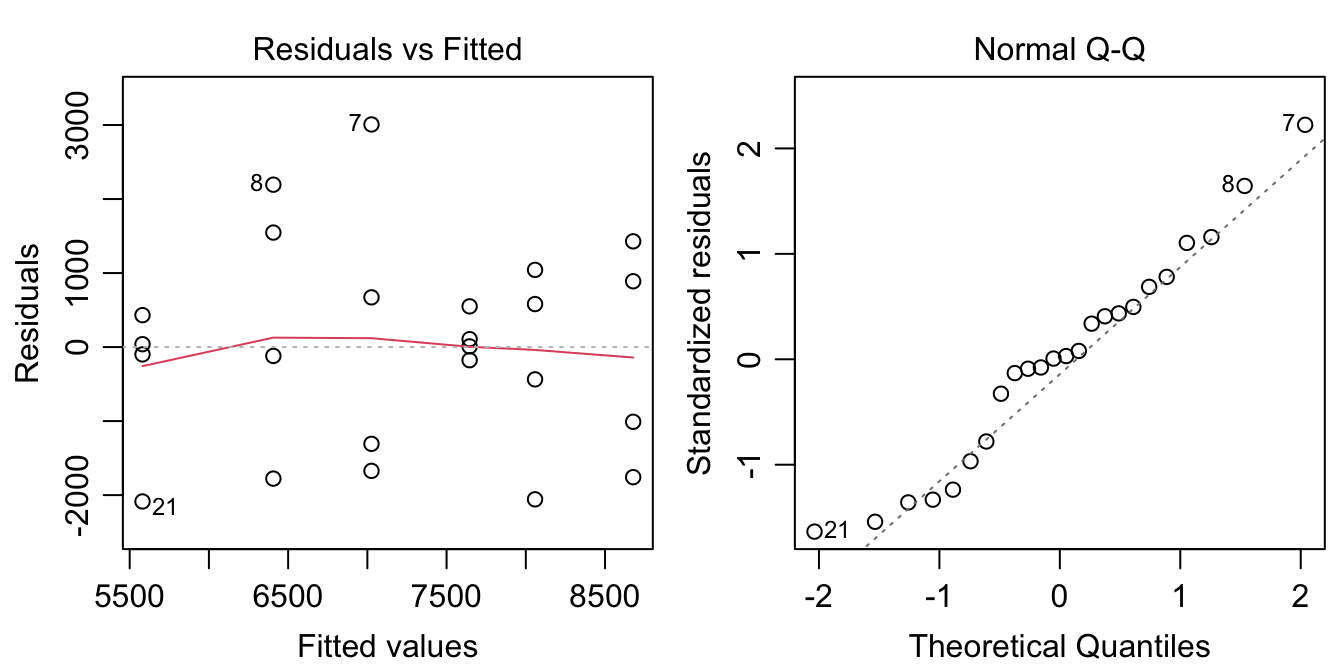
\includegraphics{Rstats4ag_files/figure-latex/figbeetdensdiag-1.pdf}
\caption{\label{fig:figbeetdensdiag}\emph{Model diagnostic plots for linear model of sugarbeet yield as a function of volunteer corn density.}}
\end{figure}

We can also conduct a lack-of-fit test to be sure a linear model is appropriate. The simplest way to do this is to fit a linear model that removes the linear structure of the independent variable (treating it as a factor variable). The models can then be compared using the \texttt{anova()} function.

\begin{Shaded}
\begin{Highlighting}[]
\NormalTok{density.lm2 <-}\StringTok{ }\KeywordTok{lm}\NormalTok{(LbsSucA }\OperatorTok{~}\StringTok{ }\KeywordTok{as.factor}\NormalTok{(Density), }\DataTypeTok{data =}\NormalTok{ beets.dat)}
\KeywordTok{anova}\NormalTok{(density.lm, density.lm2)}
\end{Highlighting}
\end{Shaded}

\begin{verbatim}
## Analysis of Variance Table
## 
## Model 1: LbsSucA ~ Density
## Model 2: LbsSucA ~ as.factor(Density)
##   Res.Df      RSS Df Sum of Sq      F Pr(>F)
## 1     22 42066424                           
## 2     18 40058981  4   2007444 0.2255 0.9206
\end{verbatim}

When 2 linear models are provided to the \texttt{anova()} function, the models will be compared using an F-test. This is only appropriate when the models are nested; that is, one model is a reduced form of the other. The highly non-significant p-value above (p = 0.92) indicates that removing the structured nature of the density variable does not increase the model fit. Therefore, we will proceed with the regression analysis.

\hypertarget{model-interpretation}{%
\subsection{Model Interpretation}\label{model-interpretation}}

Using the \texttt{anova()} function on a a single fitted lm object produces output similar to the \texttt{aov()} function. The ANOVA table indicates strong evidence that volunteer corn density has an effect on the sugar production, as expected. To get the regression equation, we use the \texttt{summary()} function on the fitted lm model:

\begin{Shaded}
\begin{Highlighting}[]
\KeywordTok{anova}\NormalTok{(density.lm)}
\end{Highlighting}
\end{Shaded}

\begin{verbatim}
## Analysis of Variance Table
## 
## Response: LbsSucA
##           Df   Sum Sq  Mean Sq F value   Pr(>F)   
## Density    1 25572276 25572276  13.374 0.001387 **
## Residuals 22 42066424  1912110                    
## ---
## Signif. codes:  0 '***' 0.001 '**' 0.01 '*' 0.05 '.' 0.1 ' ' 1
\end{verbatim}

\begin{Shaded}
\begin{Highlighting}[]
\KeywordTok{summary}\NormalTok{(density.lm)}
\end{Highlighting}
\end{Shaded}

\begin{verbatim}
## 
## Call:
## lm(formula = LbsSucA ~ Density, data = beets.dat)
## 
## Residuals:
##      Min       1Q   Median       3Q      Max 
## -2086.02 -1084.01    23.92   726.23  3007.73 
## 
## Coefficients:
##             Estimate Std. Error t value Pr(>|t|)    
## (Intercept)   8677.6      485.6  17.869 1.38e-14 ***
## Density     -20644.7     5645.2  -3.657  0.00139 ** 
## ---
## Signif. codes:  0 '***' 0.001 '**' 0.01 '*' 0.05 '.' 0.1 ' ' 1
## 
## Residual standard error: 1383 on 22 degrees of freedom
## Multiple R-squared:  0.3781, Adjusted R-squared:  0.3498 
## F-statistic: 13.37 on 1 and 22 DF,  p-value: 0.001387
\end{verbatim}

The resulting output provides estimates for the intercept (8678), and slope (-20645) of the regression line under the heading ``Coefficients.'' The \texttt{summary()} function also prints standard errors, t-statistics, and P-values, and fit statistics such as the R\textsuperscript{2} for these estimates are also provided. The regression line for this example would be:

Y = 8678 - 20645*X

To plot the data along with the fitted line:



\begin{Shaded}
\begin{Highlighting}[]
\KeywordTok{par}\NormalTok{(}\DataTypeTok{mfrow=}\KeywordTok{c}\NormalTok{(}\DecValTok{1}\NormalTok{,}\DecValTok{1}\NormalTok{), }\DataTypeTok{mar=}\KeywordTok{c}\NormalTok{(}\FloatTok{3.2}\NormalTok{,}\FloatTok{3.2}\NormalTok{,}\DecValTok{2}\NormalTok{,.}\DecValTok{5}\NormalTok{), }\DataTypeTok{mgp=}\KeywordTok{c}\NormalTok{(}\DecValTok{2}\NormalTok{,.}\DecValTok{7}\NormalTok{,}\DecValTok{0}\NormalTok{))}
\KeywordTok{plot}\NormalTok{(beets.dat}\OperatorTok{$}\NormalTok{LbsSucA }\OperatorTok{~}\StringTok{ }\NormalTok{beets.dat}\OperatorTok{$}\NormalTok{Density, }\DataTypeTok{bty=}\StringTok{"l"}\NormalTok{,}
     \DataTypeTok{ylab=}\StringTok{"Sugar yield (lbs/A)"}\NormalTok{, }\DataTypeTok{xlab=}\StringTok{"Volunteer corn density (plants/ft row)"}\NormalTok{,}
     \DataTypeTok{main=}\StringTok{"Lingle, WY 2009"}\NormalTok{, }\DataTypeTok{ylim=}\KeywordTok{c}\NormalTok{(}\DecValTok{0}\NormalTok{,}\DecValTok{10000}\NormalTok{))}
  \KeywordTok{abline}\NormalTok{(density.lm) }\CommentTok{# Add the regression line}
\CommentTok{# to add the regression equation into the plot:}
\NormalTok{  int<-}\KeywordTok{round}\NormalTok{(}\KeywordTok{summary}\NormalTok{(density.lm)}\OperatorTok{$}\NormalTok{coefficients[[}\DecValTok{1}\NormalTok{]]) }\CommentTok{# get intercept}
\NormalTok{  sl<-}\StringTok{ }\KeywordTok{round}\NormalTok{(}\KeywordTok{summary}\NormalTok{(density.lm)}\OperatorTok{$}\NormalTok{coefficients[[}\DecValTok{2}\NormalTok{]]) }\CommentTok{# get slope}
\NormalTok{  reg.eq<-}\KeywordTok{paste}\NormalTok{(}\StringTok{"Y ="}\NormalTok{, int, sl, }\StringTok{"* X"}\NormalTok{) }\CommentTok{# create text regression equation}
  \KeywordTok{legend}\NormalTok{(}\StringTok{"bottomleft"}\NormalTok{,reg.eq, }\DataTypeTok{bty=}\StringTok{"n"}\NormalTok{)}
\end{Highlighting}
\end{Shaded}

\begin{figure}
\centering
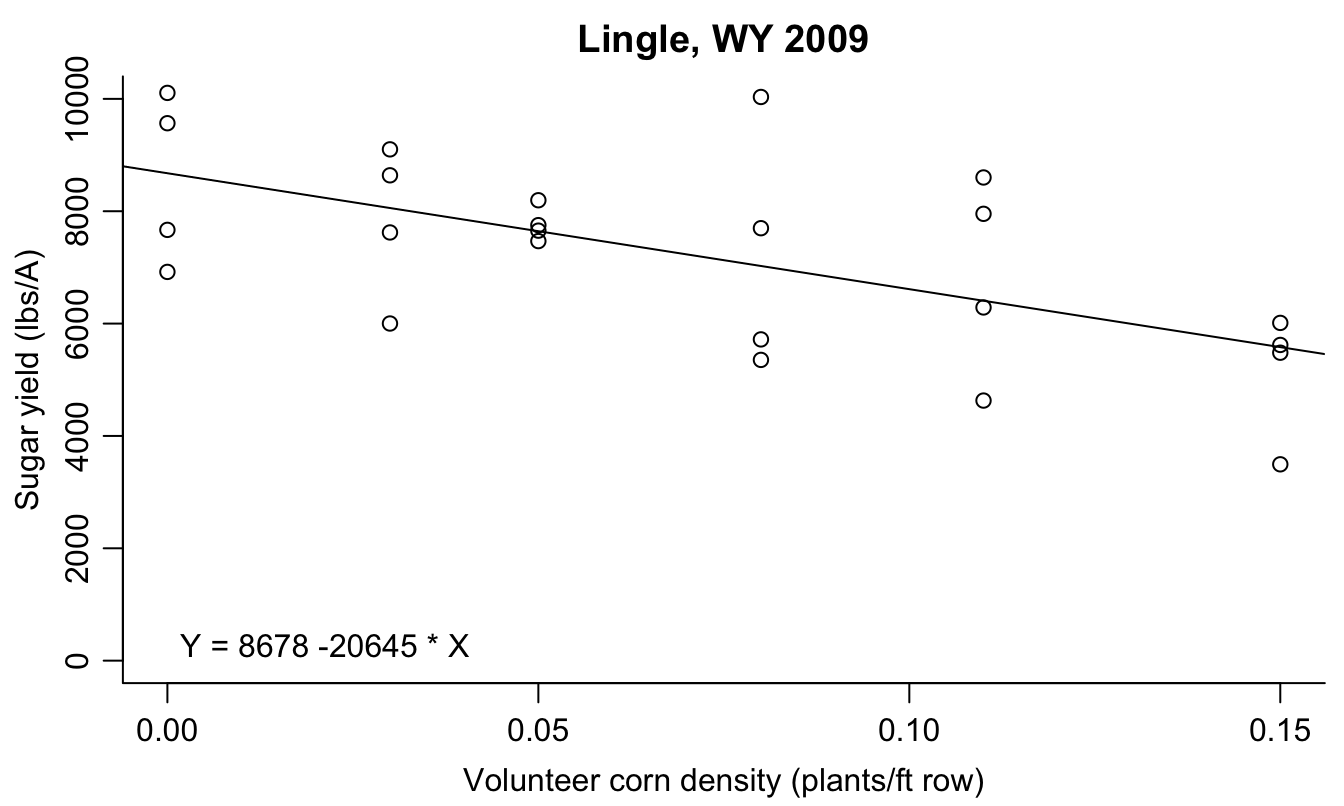
\includegraphics{Rstats4ag_files/figure-latex/figbeetdens-1.pdf}
\caption{\label{fig:figbeetdens}\emph{Effect of volunteer corn density on sugarbeet yield.}}
\end{figure}

The sugar yield was decreased by 20,600 lbs/A for each volunteer corn plant per foot of sugarbeet row; this seems unintuitive since the Y-intercept was only 8,678 lbs/A. The maximum volunteer corn density used in the study was only 0.15 plants per foot of sugarbeet row, so the units of the slope are not directly applicable to the data observed in the study. Although the linear regression model is appropriate here, it is extremely important \emph{not} to extrapolate the linear model results to volunteer corn densities outside the observed data range (densities greater than 0.15 plants per foot of row). This can be illustrated by changing the Y and X limits on the figure. If extrapolation is absolutely necessary, a nonlinear model would be more appropriate (although still not ideal). The ideal situation would be to repeat the study with weed densities that caused crop yield to drop close to the minimum yield.



\begin{figure}
\centering
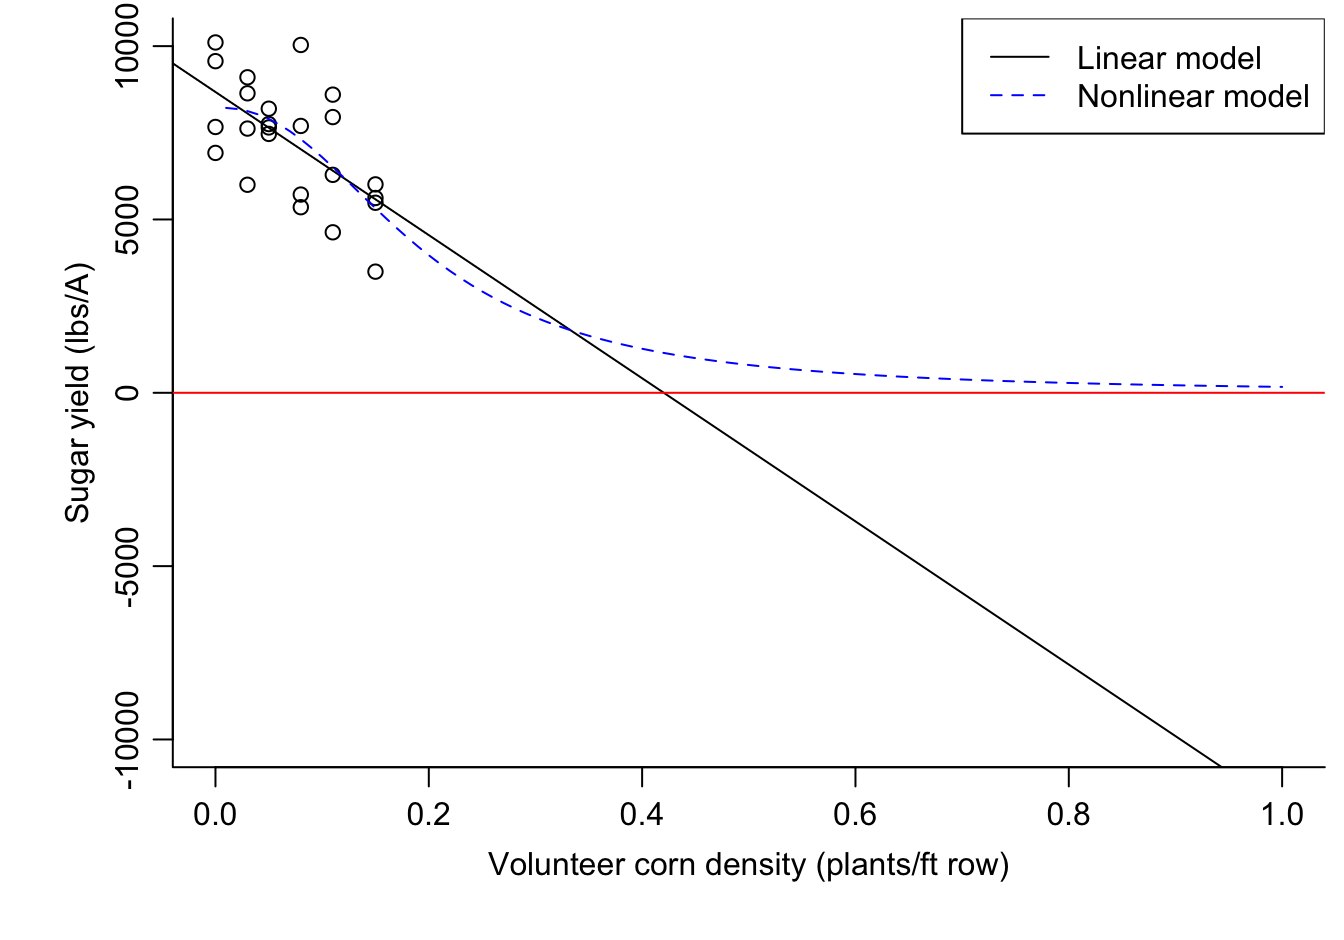
\includegraphics{Rstats4ag_files/figure-latex/figbeetlmvsnlin-1.pdf}
\caption{\label{fig:figbeetlmvsnlin}\emph{Linear model vs nonlinear model for sugarbeet response to volunteer corn density.}}
\end{figure}

\begin{center}\rule{0.5\linewidth}{0.5pt}\end{center}

\hypertarget{analysis-of-covariance-ancova}{%
\chapter{Analysis of Covariance (ANCOVA)}\label{analysis-of-covariance-ancova}}

In an ANOVA the interest lies in the differences among means. In a linear regression the interest lies in the intercept and slope parameters of regression lines, or perhaps other parameters of biological interest, e.g.~asymptotic and effective doses (e.g, \(latex LD_{50}\) levels in the nonlinear case. The combination of ANOVA and regression is called Analysis of Covariance (ANCOVA). It is an underutilized method that makes sequential tests for testing various hypotheses. Usually it is confined to linear regressions but can be equally powerful when used in nonlinear relationships. However, in this section we only consider the linear ANCOVA.

\hypertarget{example-1-mechanical-weed-control}{%
\section{Example 1: Mechanical Weed Control}\label{example-1-mechanical-weed-control}}

A mechanical weed control experiment (\href{http://onlinelibrary.wiley.com/doi/10.1111/j.1365-3180.2008.00661.x/full}{Rasmussen et al.~2008}{]} tested the effect of intensity of harrowing (1, 2, 3, or 4 times), either along or across the direction of sowing (factors) on the weed cover left after the harrowing.

\begin{Shaded}
\begin{Highlighting}[]
\NormalTok{Harrowing<-}\StringTok{ }\KeywordTok{read.csv2}\NormalTok{(}\StringTok{"http://rstats4ag.org/data/Harrowing.csv"}\NormalTok{)}
\KeywordTok{head}\NormalTok{(Harrowing,}\DecValTok{3}\NormalTok{)}
\end{Highlighting}
\end{Shaded}

\begin{verbatim}
##   plot       leaf     weeds int direction yield
## 1    1 0.18623052 103.33763   0     along  4.21
## 2    2 0.12696533  54.02022   1     along  4.08
## 3    3 0.09006582  23.44035   2     along  3.92
\end{verbatim}

Lets look at the relationships in Figure \ref{fig:figharrowpanel}.



\begin{Shaded}
\begin{Highlighting}[]
\KeywordTok{library}\NormalTok{(lattice)}
\KeywordTok{xyplot}\NormalTok{(weeds }\OperatorTok{~}\StringTok{ }\NormalTok{int }\OperatorTok{|}\StringTok{ }\NormalTok{direction, }\DataTypeTok{data =}\NormalTok{ Harrowing,}
       \DataTypeTok{ylab=}\StringTok{"Weed Cover"}\NormalTok{,}\DataTypeTok{xlab=}\StringTok{"Intensity of Harrowing"}\NormalTok{  )     }
\end{Highlighting}
\end{Shaded}

\begin{figure}
\centering
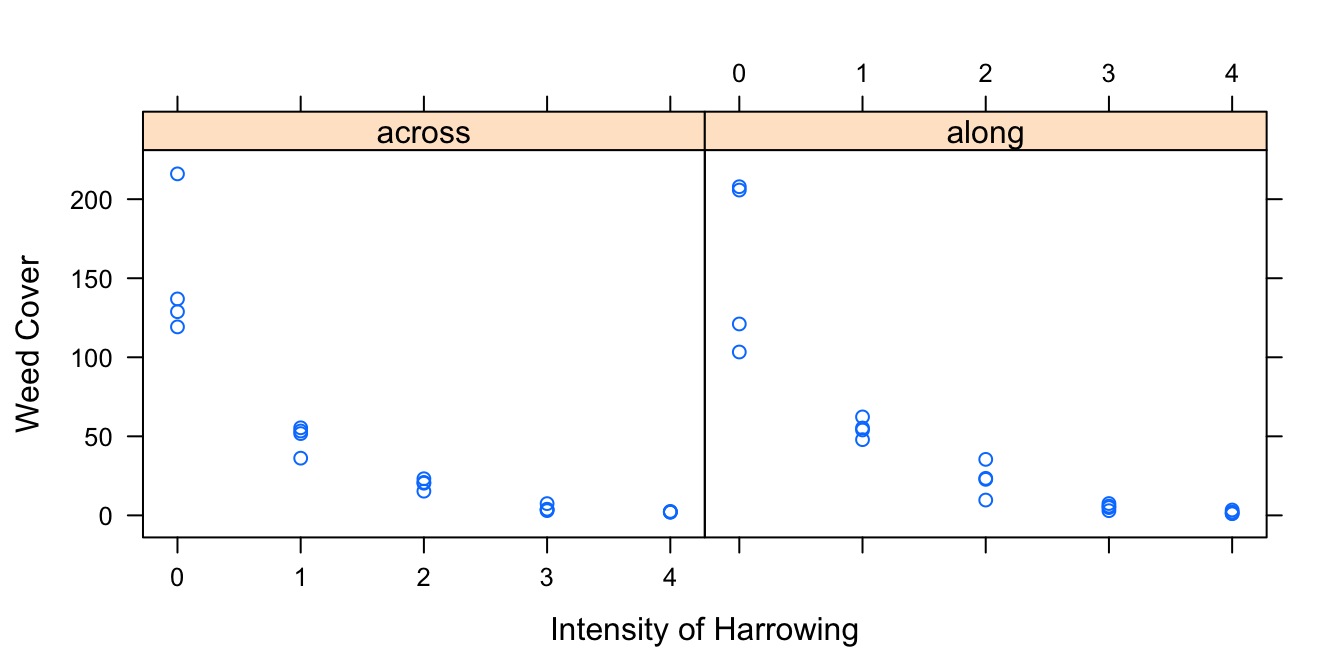
\includegraphics{Rstats4ag_files/figure-latex/figharrowpanel-1.pdf}
\caption{\label{fig:figharrowpanel}\emph{The relationship between weed cover and intensity of harrowing either across or along the direction of sowing.}}
\end{figure}

The relationships above does not look very linear, it looks like an exponential decreasing leaf cover. If this assumption is correct we can make the relationship linear by taking the logarithm of weed cover.



\begin{Shaded}
\begin{Highlighting}[]
\KeywordTok{xyplot}\NormalTok{(}\KeywordTok{log}\NormalTok{(weeds) }\OperatorTok{~}\StringTok{ }\NormalTok{int }\OperatorTok{|}\StringTok{ }\NormalTok{direction, }\DataTypeTok{data =}\NormalTok{ Harrowing,}
       \DataTypeTok{ylab=}\StringTok{"Log(Weed Cover)"}\NormalTok{,}\DataTypeTok{xlab=}\StringTok{"Intensity of Harrowing"}\NormalTok{,}
       \DataTypeTok{panel =} \ControlFlowTok{function}\NormalTok{(x,y)}
\NormalTok{       \{}\KeywordTok{panel.xyplot}\NormalTok{(x,y)}
        \KeywordTok{panel.lmline}\NormalTok{(x,y)\})}
\end{Highlighting}
\end{Shaded}

\begin{figure}
\centering
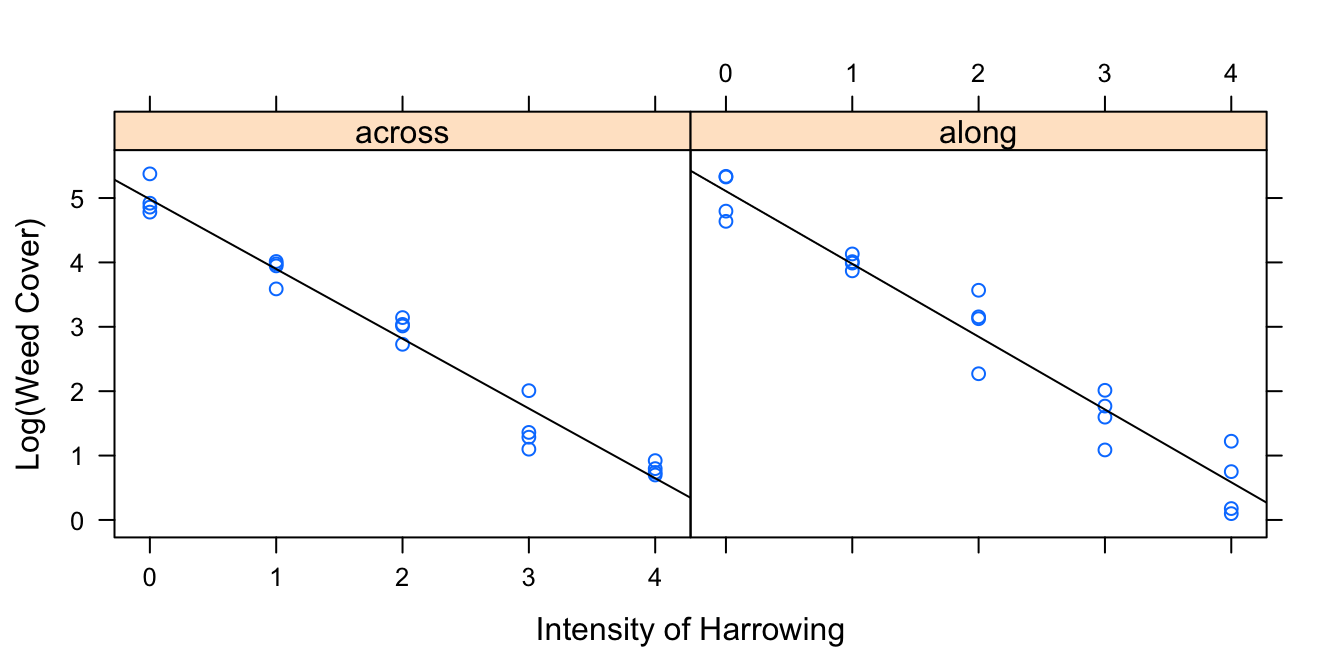
\includegraphics{Rstats4ag_files/figure-latex/figharrowpanellog-1.pdf}
\caption{\label{fig:figharrowpanellog}\emph{Same data as in \ref{fig:figharrowpanel} using the logarithm of weed cover (y-axis) gives a relationship that looks linear on the intensity of harrowing within the directions of harrowing.}}
\end{figure}

Apparently, the assumption of a straight line relationship looks good, but we have to do statistics to substantiate this hypothesis. It is of interest to know whether the harrowing direction (across or along the rows) had the same effect on weed cover. Statistically, we want to know if the two regression lines are similar in term of regression slopes. This can be done by sequential testing:

\begin{itemize}
\tightlist
\item
  Ordinary ANOVA where \texttt{int} is turned into a factor \texttt{factor(int)}
\item
  ANCOVA with interaction; meaning that the regression lines can have both different slopes and intercepts
\end{itemize}

\begin{Shaded}
\begin{Highlighting}[]
\NormalTok{Harrowing}\OperatorTok{$}\NormalTok{Log.weeds <-}\StringTok{ }\KeywordTok{log}\NormalTok{(Harrowing}\OperatorTok{$}\NormalTok{weeds)}
\NormalTok{m1 <-}\StringTok{ }\KeywordTok{lm}\NormalTok{(Log.weeds }\OperatorTok{~}\StringTok{ }\KeywordTok{factor}\NormalTok{(int) }\OperatorTok{*}\StringTok{ }\NormalTok{direction, }\DataTypeTok{data =}\NormalTok{ Harrowing)}
\NormalTok{m2 <-}\StringTok{ }\KeywordTok{lm}\NormalTok{(Log.weeds }\OperatorTok{~}\StringTok{ }\NormalTok{int }\OperatorTok{*}\StringTok{ }\NormalTok{direction, }\DataTypeTok{data =}\NormalTok{ Harrowing)}
\KeywordTok{anova}\NormalTok{(m1, m2)}
\end{Highlighting}
\end{Shaded}

\begin{verbatim}
## Analysis of Variance Table
## 
## Model 1: Log.weeds ~ factor(int) * direction
## Model 2: Log.weeds ~ int * direction
##   Res.Df    RSS Df Sum of Sq      F Pr(>F)
## 1     30 3.5350                           
## 2     36 4.2754 -6  -0.74048 1.0474 0.4152
\end{verbatim}

\texttt{m1}, an ordinary ANOVA, is the most general model with no assumption of any particular relationship. \texttt{m2}is the ANCOCVA, which assumes there is a linear relationship between harrowing direction and intensity. The \texttt{int\ *\ direction} in \texttt{m2} means that there is an interaction between the slopes depending on the direction of harrowing. Or in other words the slopes of the regression lines are different. The test for lack of fit is not significant (p=0.42) so we can assume a linear relationship applies to the log-transformed response variable.

We can further refine the analysis through sequential testing:
* Assuming similar slope but different intercept depending of direction of harrowing
* Assuming that the directions of harrowing does not influence regression lines, e.i, similar line

To do this, we first test the regression model with an interaction term, \texttt{m2}, with a regression model where we assume no interaction,\texttt{m3}, which mean the slopes of the regression lines are similar:

\begin{Shaded}
\begin{Highlighting}[]
\NormalTok{m3 <-}\StringTok{ }\KeywordTok{lm}\NormalTok{(Log.weeds }\OperatorTok{~}\StringTok{ }\NormalTok{int }\OperatorTok{+}\StringTok{ }\NormalTok{direction, }\DataTypeTok{data =}\NormalTok{ Harrowing)}
\KeywordTok{anova}\NormalTok{(m2,m3)}
\end{Highlighting}
\end{Shaded}

\begin{verbatim}
## Analysis of Variance Table
## 
## Model 1: Log.weeds ~ int * direction
## Model 2: Log.weeds ~ int + direction
##   Res.Df    RSS Df Sum of Sq      F Pr(>F)
## 1     36 4.2754                           
## 2     37 4.3207 -1 -0.045295 0.3814 0.5407
\end{verbatim}

The lack of fit test is again not significant so we can assume that there is no interaction, and conclude that the regression slopes are similar. The final test will determine whether the direction of harrowing influences the relationship between log(Weed Cover) and intensity of harrowing?

\begin{Shaded}
\begin{Highlighting}[]
\NormalTok{m4 <-}\StringTok{ }\KeywordTok{lm}\NormalTok{(Log.weeds }\OperatorTok{~}\StringTok{ }\NormalTok{int, }\DataTypeTok{data =}\NormalTok{ Harrowing)}
\KeywordTok{anova}\NormalTok{(m4, m3)}
\end{Highlighting}
\end{Shaded}

\begin{verbatim}
## Analysis of Variance Table
## 
## Model 1: Log.weeds ~ int
## Model 2: Log.weeds ~ int + direction
##   Res.Df    RSS Df Sum of Sq      F Pr(>F)
## 1     38 4.3311                           
## 2     37 4.3207  1  0.010344 0.0886 0.7677
\end{verbatim}

Again, no significance here either (p=0.77); so we end up from the most general model (ANOVA) to the most simple ANCOVA: direction of harrowing does not matter and the relationship between \texttt{log(weeds)}and intensity of harrowing is linear.

\begin{Shaded}
\begin{Highlighting}[]
\KeywordTok{summary}\NormalTok{(m4)}
\end{Highlighting}
\end{Shaded}

\begin{verbatim}
## 
## Call:
## lm(formula = Log.weeds ~ int, data = Harrowing)
## 
## Residuals:
##      Min       1Q   Median       3Q      Max 
## -0.63622 -0.25226  0.06307  0.28256  0.73686 
## 
## Coefficients:
##             Estimate Std. Error t value Pr(>|t|)    
## (Intercept)  5.04478    0.09246   54.56   <2e-16 ***
## int         -1.10710    0.03775  -29.33   <2e-16 ***
## ---
## Signif. codes:  0 '***' 0.001 '**' 0.01 '*' 0.05 '.' 0.1 ' ' 1
## 
## Residual standard error: 0.3376 on 38 degrees of freedom
## Multiple R-squared:  0.9577, Adjusted R-squared:  0.9566 
## F-statistic: 860.3 on 1 and 38 DF,  p-value: < 2.2e-16
\end{verbatim}

In order to illustrate the result we use the code below to create Figure \ref{fig:ancovaplot1}. For illustration purposes we have separated the means into direction across and along even though it is not necessary.



\begin{Shaded}
\begin{Highlighting}[]
\KeywordTok{library}\NormalTok{(dplyr)}
\NormalTok{Plot.means <-}\StringTok{ }\NormalTok{Harrowing }\OperatorTok
\StringTok{  }\KeywordTok{group_by}\NormalTok{(int, direction) }\OperatorTok
\StringTok{  }\KeywordTok{summarise}\NormalTok{(}\DataTypeTok{count =} \KeywordTok{n}\NormalTok{(), }\DataTypeTok{Log.Weeds =} \KeywordTok{mean}\NormalTok{(Log.weeds))}

\KeywordTok{par}\NormalTok{(}\DataTypeTok{mgp=}\KeywordTok{c}\NormalTok{(}\DecValTok{2}\NormalTok{,.}\DecValTok{7}\NormalTok{,}\DecValTok{0}\NormalTok{), }\DataTypeTok{mar=}\KeywordTok{c}\NormalTok{(}\FloatTok{3.2}\NormalTok{,}\FloatTok{3.2}\NormalTok{,.}\DecValTok{5}\NormalTok{,.}\DecValTok{5}\NormalTok{))}
\KeywordTok{plot}\NormalTok{(Log.Weeds}\OperatorTok{~}\NormalTok{int, }\DataTypeTok{data =}\NormalTok{ Plot.means, }\DataTypeTok{bty=}\StringTok{"l"}\NormalTok{,}
     \DataTypeTok{pch =} \KeywordTok{as.numeric}\NormalTok{(direction),}
     \DataTypeTok{xlab=}\StringTok{"Harrowing intensity"}\NormalTok{,}
     \DataTypeTok{ylab=}\StringTok{"Log(weed cover)"}\NormalTok{)}
\end{Highlighting}
\end{Shaded}

\begin{verbatim}
## Warning in FUN(X[[i]], ...): NAs introduced by coercion
\end{verbatim}

\begin{Shaded}
\begin{Highlighting}[]
\KeywordTok{abline}\NormalTok{(m4)}
\KeywordTok{legend}\NormalTok{(}\StringTok{"bottomleft"}\NormalTok{, }\KeywordTok{c}\NormalTok{(}\StringTok{"Across"}\NormalTok{, }\StringTok{"Along"}\NormalTok{), }\DataTypeTok{pch =} \KeywordTok{c}\NormalTok{(}\DecValTok{2}\NormalTok{,}\DecValTok{1}\NormalTok{))}
\end{Highlighting}
\end{Shaded}

\begin{figure}
\centering
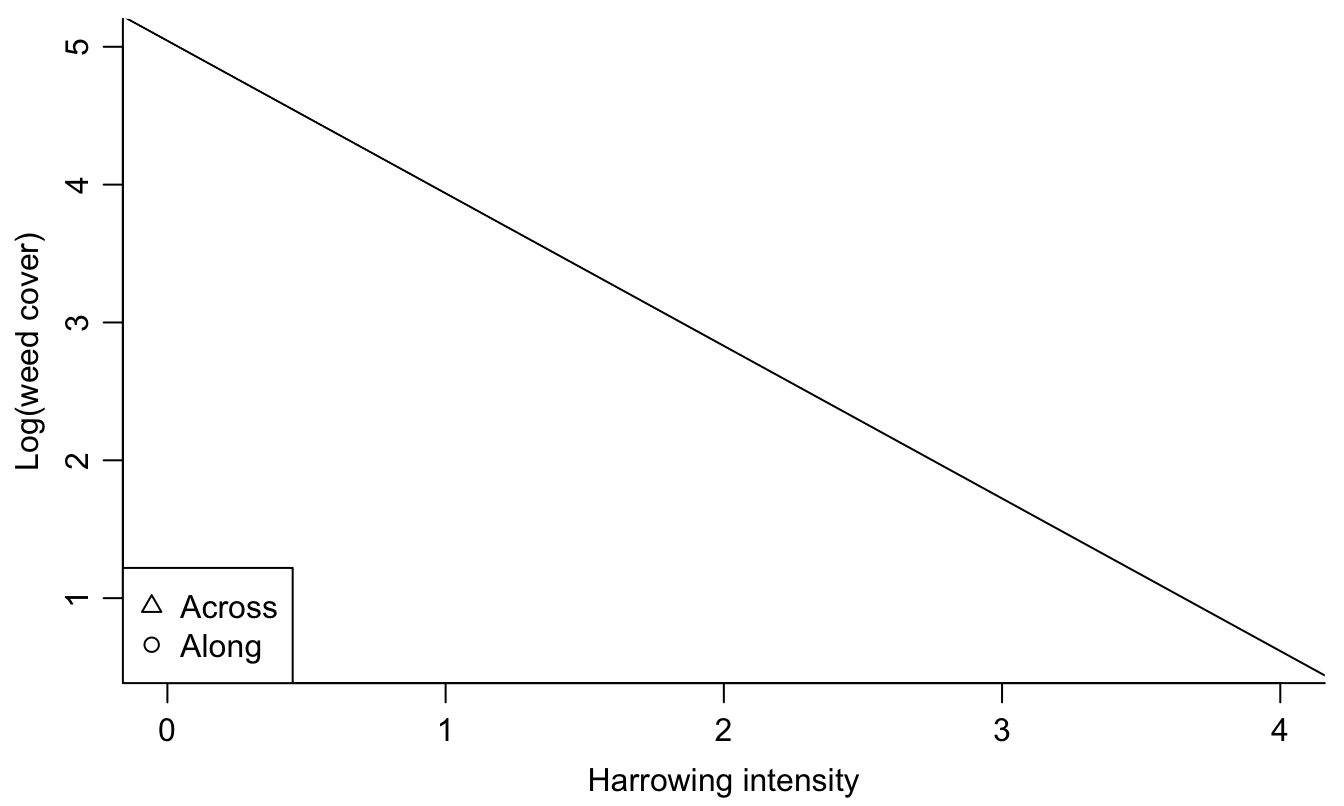
\includegraphics{Rstats4ag_files/figure-latex/ancovaplot1-1.pdf}
\caption{\label{fig:ancovaplot1}\emph{Summary plot of the harrowing experiments. There is no difference between the direction of harrowing and, therefore, only one regression line is necessary.}}
\end{figure}

The slope is -1.11 (0.04) which means that with an increase in harrowing intensity the logarithm of weed cover decreases by -1.11. In fact the relationship is an exponential decay curve where the relative rate of change is exp(-1.11)= 0.3296 wherever we are on the curve.

\hypertarget{example-2-duration-of-competition}{%
\section{Example 2: Duration of competition}\label{example-2-duration-of-competition}}

In 2006 and 2007, field studies were conducted near Powell, Wyoming to determine the effects of Salvia reflexa (lanceleaf sage) interference with sugarbeet. This data was published in \href{http://www.bioone.org/doi/abs/10.1614/WT-D-10-00015.1}{Odero et al.~2010}. Salvia reflexa was seeded alongside the sugarbeet crop at a constant density, and allowed to compete for time periods ranging from 36 to 133 days after sugarbeet emergence. Yields (\texttt{Yield\_Mg.ha}) were determined at the end of the season.

\begin{Shaded}
\begin{Highlighting}[]
\NormalTok{lanceleaf.sage<-}\KeywordTok{read.csv}\NormalTok{(}\StringTok{"http://rstats4ag.org/data/lanceleafsage.csv"}\NormalTok{)}
\KeywordTok{head}\NormalTok{(lanceleaf.sage,}\DataTypeTok{n=}\DecValTok{3}\NormalTok{)}
\end{Highlighting}
\end{Shaded}

\begin{verbatim}
##   Replicate Duration Year Yield_Mg.ha Yield.loss.pct
## 1         1       36 2006       67.26          98.05
## 2         1       50 2006       60.34          87.96
## 3         1       64 2006       53.69          78.27
\end{verbatim}



\begin{Shaded}
\begin{Highlighting}[]
\KeywordTok{library}\NormalTok{(lattice)}
\KeywordTok{xyplot}\NormalTok{(Yield_Mg.ha}\OperatorTok{~}\NormalTok{Duration}\OperatorTok{|}\KeywordTok{factor}\NormalTok{(Year),}\DataTypeTok{data=}\NormalTok{lanceleaf.sage,}
        \DataTypeTok{ylab=} \StringTok{"Sugarbeet root yield (t/ha)"}\NormalTok{,}
        \DataTypeTok{xlab=}\StringTok{"Duration of competition from _Salvia reflexa_"}\NormalTok{,}
        \DataTypeTok{panel =} \ControlFlowTok{function}\NormalTok{(x,y)}
\NormalTok{       \{}\KeywordTok{panel.xyplot}\NormalTok{(x,y)}
        \KeywordTok{panel.lmline}\NormalTok{(x,y)\})}
\end{Highlighting}
\end{Shaded}

\begin{figure}
\centering
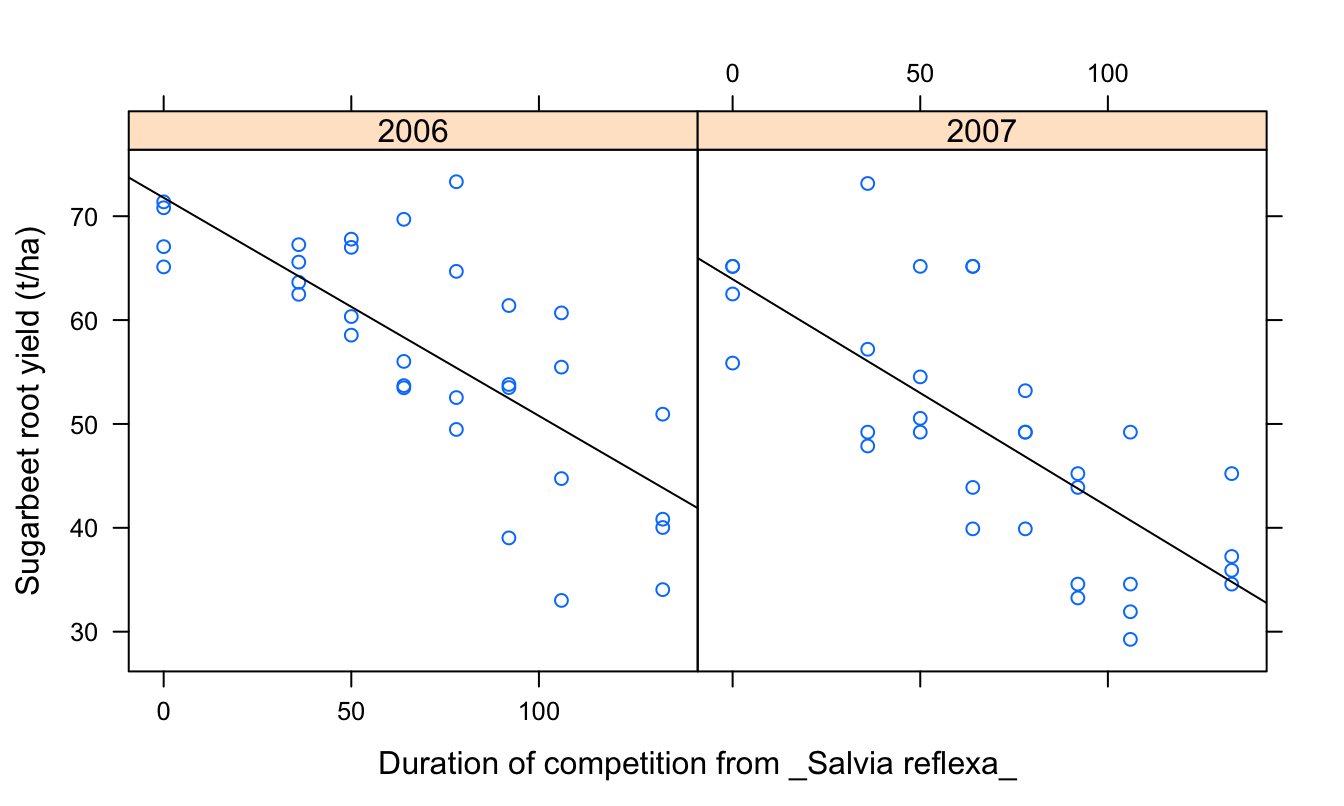
\includegraphics{Rstats4ag_files/figure-latex/figsagepanel-1.pdf}
\caption{\label{fig:figsagepanel}\emph{Duration of} Salvia reflexa \emph{competition effect on yield of sugar beet in two years.}}
\end{figure}

As was the case with the harrowing experiment we do sequential testing. First, we compare the ANCOVA with the most general model, an AVOVA:

\begin{Shaded}
\begin{Highlighting}[]
\NormalTok{lm1 <-}\StringTok{ }\KeywordTok{lm}\NormalTok{(Yield_Mg.ha }\OperatorTok{~}\StringTok{ }\KeywordTok{factor}\NormalTok{(Duration) }\OperatorTok{*}\StringTok{ }\KeywordTok{factor}\NormalTok{(Year), }\DataTypeTok{data =}\NormalTok{ lanceleaf.sage) }\CommentTok{# ANOVA}
\NormalTok{lm2 <-}\StringTok{ }\KeywordTok{lm}\NormalTok{(Yield_Mg.ha }\OperatorTok{~}\StringTok{ }\NormalTok{Duration }\OperatorTok{*}\StringTok{ }\KeywordTok{factor}\NormalTok{(Year), }\DataTypeTok{data =}\NormalTok{ lanceleaf.sage) }\CommentTok{# Regression}
\KeywordTok{anova}\NormalTok{(lm1, lm2) }\CommentTok{# Lack of fit test}
\end{Highlighting}
\end{Shaded}

\begin{verbatim}
## Analysis of Variance Table
## 
## Model 1: Yield_Mg.ha ~ factor(Duration) * factor(Year)
## Model 2: Yield_Mg.ha ~ Duration * factor(Year)
##   Res.Df    RSS  Df Sum of Sq      F Pr(>F)
## 1     48 3198.3                            
## 2     60 3667.1 -12   -468.78 0.5863 0.8423
\end{verbatim}

The test for lack of fit shows that we can safely assume a linear regression (p=0.84). The next step is to test if we can assume similar slopes for the regression in the two years.

\begin{Shaded}
\begin{Highlighting}[]
\NormalTok{lm3 <-}\StringTok{ }\KeywordTok{lm}\NormalTok{(Yield_Mg.ha }\OperatorTok{~}\StringTok{ }\NormalTok{Duration }\OperatorTok{+}\StringTok{ }\KeywordTok{factor}\NormalTok{(Year), }\DataTypeTok{data =}\NormalTok{ lanceleaf.sage)}
\KeywordTok{anova}\NormalTok{(lm2, lm3) }
\end{Highlighting}
\end{Shaded}

\begin{verbatim}
## Analysis of Variance Table
## 
## Model 1: Yield_Mg.ha ~ Duration * factor(Year)
## Model 2: Yield_Mg.ha ~ Duration + factor(Year)
##   Res.Df    RSS Df Sum of Sq      F Pr(>F)
## 1     60 3667.1                           
## 2     61 3669.1 -1   -2.0366 0.0333 0.8558
\end{verbatim}

Again we can confidently assume that the slopes are the same irrespective of year (p=0.86). The next question: are the regression lines identical?

\begin{Shaded}
\begin{Highlighting}[]
\NormalTok{lm4 <-}\StringTok{ }\KeywordTok{lm}\NormalTok{(Yield_Mg.ha }\OperatorTok{~}\StringTok{ }\NormalTok{Duration, }\DataTypeTok{data =}\NormalTok{ lanceleaf.sage)}
\KeywordTok{anova}\NormalTok{(lm4, lm3) }
\end{Highlighting}
\end{Shaded}

\begin{verbatim}
## Analysis of Variance Table
## 
## Model 1: Yield_Mg.ha ~ Duration
## Model 2: Yield_Mg.ha ~ Duration + factor(Year)
##   Res.Df    RSS Df Sum of Sq      F    Pr(>F)    
## 1     62 4819.3                                  
## 2     61 3669.1  1    1150.2 19.123 4.862e-05 ***
## ---
## Signif. codes:  0 '***' 0.001 '**' 0.01 '*' 0.05 '.' 0.1 ' ' 1
\end{verbatim}

We get a extremely low p value (p\textless{}0.0001). Therefore, the reduced model significantly reduces the fit. In other words, the \texttt{lm3} model is the model that should be used to summarize the experiment.

\begin{Shaded}
\begin{Highlighting}[]
\KeywordTok{summary}\NormalTok{(lm3)}
\end{Highlighting}
\end{Shaded}

\begin{verbatim}
## 
## Call:
## lm(formula = Yield_Mg.ha ~ Duration + factor(Year), data = lanceleaf.sage)
## 
## Residuals:
##      Min       1Q   Median       3Q      Max 
## -16.3477  -5.2428  -0.7246   3.5724  17.9560 
## 
## Coefficients:
##                  Estimate Std. Error t value Pr(>|t|)    
## (Intercept)      72.09580    2.20523  32.693  < 2e-16 ***
## Duration         -0.21451    0.02472  -8.678 3.02e-12 ***
## factor(Year)2007 -8.47875    1.93890  -4.373 4.86e-05 ***
## ---
## Signif. codes:  0 '***' 0.001 '**' 0.01 '*' 0.05 '.' 0.1 ' ' 1
## 
## Residual standard error: 7.756 on 61 degrees of freedom
## Multiple R-squared:  0.6075, Adjusted R-squared:  0.5947 
## F-statistic: 47.21 on 2 and 61 DF,  p-value: 4.081e-13
\end{verbatim}

```

The slopes are similar but not the intercepts and the summary of the experiment can be neatly presented graphically in Figure \ref{fig:figsageresults}.



\begin{Shaded}
\begin{Highlighting}[]
\KeywordTok{library}\NormalTok{(dplyr)}
\NormalTok{averages<-lanceleaf.sage }\OperatorTok
\StringTok{  }\KeywordTok{group_by}\NormalTok{(Duration, Year) }\OperatorTok
\StringTok{  }\KeywordTok{summarise}\NormalTok{(}\DataTypeTok{count =} \KeywordTok{n}\NormalTok{(), }\DataTypeTok{YIELD =} \KeywordTok{mean}\NormalTok{(Yield_Mg.ha))}

\KeywordTok{par}\NormalTok{(}\DataTypeTok{mar=}\KeywordTok{c}\NormalTok{(}\FloatTok{3.2}\NormalTok{,}\FloatTok{3.2}\NormalTok{,.}\DecValTok{5}\NormalTok{,.}\DecValTok{5}\NormalTok{), }\DataTypeTok{mgp=}\KeywordTok{c}\NormalTok{(}\DecValTok{2}\NormalTok{,.}\DecValTok{7}\NormalTok{,}\DecValTok{0}\NormalTok{))}
\KeywordTok{plot}\NormalTok{(YIELD }\OperatorTok{~}\StringTok{ }\NormalTok{Duration, }\DataTypeTok{data =}\NormalTok{ averages, }\DataTypeTok{bty=}\StringTok{"l"}\NormalTok{,}
     \DataTypeTok{pch =} \KeywordTok{as.numeric}\NormalTok{(}\KeywordTok{factor}\NormalTok{(Year)), }\DataTypeTok{ylim=}\KeywordTok{c}\NormalTok{(}\DecValTok{10}\NormalTok{, }\DecValTok{80}\NormalTok{), }
     \DataTypeTok{ylab=}\StringTok{"Sugarbeet root yield (t/ha)"}\NormalTok{,}
     \DataTypeTok{xlab=}\StringTok{"Duration of competition from Salvia reflexa"}\NormalTok{)}
\NormalTok{x <-}\StringTok{ }\KeywordTok{c}\NormalTok{(}\DecValTok{0}\NormalTok{, }\DecValTok{300}\NormalTok{)}\CommentTok{#dummy intensities}
\KeywordTok{lines}\NormalTok{(x, }\KeywordTok{predict}\NormalTok{(lm3, }\DataTypeTok{newdata =} \KeywordTok{data.frame}\NormalTok{(}\DataTypeTok{Year =} \StringTok{"2006"}\NormalTok{,}
                                        \DataTypeTok{Duration =}\NormalTok{ x)), }\DataTypeTok{lty =} \DecValTok{2}\NormalTok{)}
\KeywordTok{lines}\NormalTok{(x, }\KeywordTok{predict}\NormalTok{(lm3, }\DataTypeTok{newdata =} \KeywordTok{data.frame}\NormalTok{(}\DataTypeTok{Year =} \StringTok{"2007"}\NormalTok{,}
                                          \DataTypeTok{Duration =}\NormalTok{ x)), }\DataTypeTok{lty =} \DecValTok{1}\NormalTok{)}
\KeywordTok{legend}\NormalTok{(}\StringTok{"topright"}\NormalTok{, }\KeywordTok{c}\NormalTok{(}\StringTok{"2006"}\NormalTok{, }\StringTok{"2007"}\NormalTok{), }\DataTypeTok{lty =} \KeywordTok{c}\NormalTok{(}\DecValTok{2}\NormalTok{, }\DecValTok{1}\NormalTok{),}
       \DataTypeTok{pch =} \KeywordTok{c}\NormalTok{(}\DecValTok{1}\NormalTok{,}\DecValTok{2}\NormalTok{),   }\DataTypeTok{merge =} \OtherTok{TRUE}\NormalTok{)}
\end{Highlighting}
\end{Shaded}

\begin{figure}
\centering
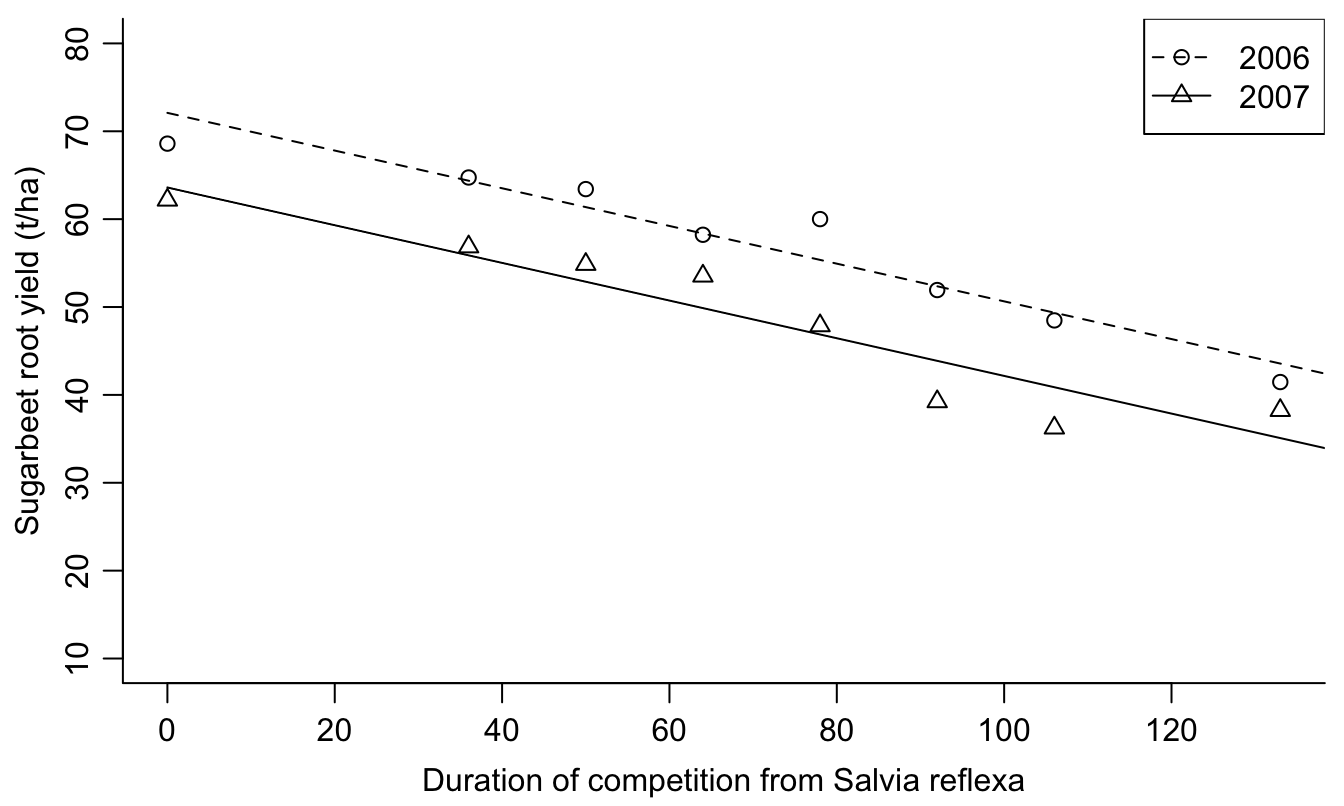
\includegraphics{Rstats4ag_files/figure-latex/figsageresults-1.pdf}
\caption{\label{fig:figsageresults}\emph{Sugarbeet yield in response to duration of} Salvia reflexa \emph{competition.}}
\end{figure}

Note the codes to obtain the regression lines for each year are more involved that in the harrowing example in Figure \ref{fig:ancovaplot1}. You must separate the regression lines on the basis of \texttt{Year} and define an independent variable \texttt{x}. Since it is a strait line you only need two `x's within year to draw the lines.

Even though the maximum yield (y-intercept) was different between years (72.1 in 2006 compared with 63.6 in 2007), yield reduction was similar in response to duration of weed competition. Each day of competition reduced the yield by 0.21 tons/ha (slope= -0.215 (0.025)).

\begin{center}\rule{0.5\linewidth}{0.5pt}\end{center}

\hypertarget{mixed-models---anova}{%
\chapter{Mixed Models - ANOVA}\label{mixed-models---anova}}

There are many examples in agronomy and weed science where mixed effects models are appropriate. In ANOVA, everything except the intentional (fixed) treatment(s), reflect random variation. This includes soil variability, experimental locations, benches in the greenhouse, weather patterns between years; many things can affect experimental results that simply cannot be controlled. In many cases, we can try to account for these sources of variation by blocking. We can consider the selection of the blocks to take place at random in the sense that we usually cannot tell in advance whether or not the next block will exhibit a low, high, or more moderate response level. In this context, we can describe random effects as effects that cannot be controlled and therefore cannot be explained by the treatment structure of the experiment. In many designed experiments, we are not inherently interested in these random effects, but in an adequate analysis we need to acknowledge the variation that they contribute. We can do so using a mixed effects model that contains both fixed and random effects.

To illustrate mixed effects ANOVA, we will use the same dry bean herbicide data set that was used in the ANOVA section to allow for comparison; please read the ANOVA section for details on the study. We will need to load the \texttt{lme4} and \texttt{multcomp} packages for this analysis.

\begin{Shaded}
\begin{Highlighting}[]
\KeywordTok{library}\NormalTok{(lme4)}
\KeywordTok{read.csv}\NormalTok{(}\StringTok{"http://rstats4ag.org/data/FlumiBeans.csv"}\NormalTok{)->flum.dat}
\NormalTok{flum.dat}\OperatorTok{$}\NormalTok{yrblock  <-}\StringTok{ }\KeywordTok{with}\NormalTok{(flum.dat, }\KeywordTok{factor}\NormalTok{(year)}\OperatorTok{:}\KeywordTok{factor}\NormalTok{(block))}
\end{Highlighting}
\end{Shaded}

First, we can look at group means (in plants per acre, and plants per hectare) using the \texttt{dplyr} package.

\begin{Shaded}
\begin{Highlighting}[]
\KeywordTok{library}\NormalTok{(dplyr)}
\NormalTok{beansum <-}\StringTok{ }\NormalTok{flum.dat }\OperatorTok
\StringTok{  }\KeywordTok{group_by}\NormalTok{(year, treatment) }\OperatorTok
\StringTok{  }\KeywordTok{summarize}\NormalTok{( }\DataTypeTok{Pop.plantsA  =} \KeywordTok{round}\NormalTok{(}\KeywordTok{mean}\NormalTok{(population}\FloatTok{.4}\NormalTok{wk),}\OperatorTok{-}\DecValTok{2}\NormalTok{),}
             \DataTypeTok{Pop.plantsHa =} \KeywordTok{round}\NormalTok{(}\KeywordTok{mean}\NormalTok{(population}\FloatTok{.4}\NormalTok{wk}\OperatorTok{*}\FloatTok{2.47}\NormalTok{),}\OperatorTok{-}\DecValTok{2}\NormalTok{))}
\NormalTok{beansum}
\end{Highlighting}
\end{Shaded}

\begin{verbatim}
## # A tibble: 21 x 4
## # Groups:   year [3]
##     year treatment                   Pop.plantsA Pop.plantsHa
##    <int> <chr>                             <dbl>        <dbl>
##  1  2009 EPTC + ethafluralin               48800       120500
##  2  2009 flumioxazin + ethafluralin        38300        94700
##  3  2009 flumioxazin + pendimethalin       19700        48800
##  4  2009 flumioxazin + trifluralin         24400        60300
##  5  2009 Handweeded                        34800        86100
##  6  2009 imazamox + bentazon               49900       123400
##  7  2009 Nontreated                        46500       114800
##  8  2010 EPTC + ethafluralin               56600       139900
##  9  2010 flumioxazin + ethafluralin        15700        38700
## 10  2010 flumioxazin + pendimethalin       20000        49500
## # ... with 11 more rows
\end{verbatim}

\hypertarget{mixed-effects-model-using-the-lme4-package}{%
\section{Mixed Effects Model using the lme4 Package}\label{mixed-effects-model-using-the-lme4-package}}

In the ANOVA section, we considered year, block, and treatment all as fixed effects. However, because the number of replicates was different by year, analyzing the combined data from all three years is problematic. The effect of year is unbalanced; we have more observations for 2010 and 2011 than for 2009. We can deal with the unbalanced nature of the data by using a mixed effects model. There are other good reasons for analyzing the data as a mixed effect model. The hope is that the results of this experiment can be generalized beyond the three years the study was conducted. The three years in which we conducted the experiment represent 3 possible years out of many when the experiment could have been done, and therefore, we can assume the impact of year to be a random variable. Same goes for the blocking criteria within a year. However, the treatments were selected specifically to determine their impact on the dry bean crop. Therefore, we will consider the treatments as fixed effects, but the year and blocking criteria within a year random effects.

\begin{Shaded}
\begin{Highlighting}[]
\CommentTok{# Mixed Effects ANOVA}
\KeywordTok{lmer}\NormalTok{(population}\FloatTok{.4}\NormalTok{wk }\OperatorTok{~}\StringTok{ }\NormalTok{treatment}\OperatorTok{+}\NormalTok{(}\DecValTok{1}\OperatorTok{|}\NormalTok{year}\OperatorTok{/}\NormalTok{block), }\DataTypeTok{data=}\NormalTok{flum.dat, }\DataTypeTok{REML=}\NormalTok{F)->flum.lmer}
\end{Highlighting}
\end{Shaded}

\begin{verbatim}
## boundary (singular) fit: see ?isSingular
\end{verbatim}

\begin{Shaded}
\begin{Highlighting}[]
\KeywordTok{anova}\NormalTok{(flum.lmer)}
\end{Highlighting}
\end{Shaded}

\begin{verbatim}
## Analysis of Variance Table
##           npar     Sum Sq    Mean Sq F value
## treatment    6 1.1974e+10 1995718507  28.887
\end{verbatim}

\hypertarget{model-comparison-and-obtaining-p-values}{%
\subsection{Model Comparison and Obtaining P-values}\label{model-comparison-and-obtaining-p-values}}

One of the most frustrating things to many researchers analyzing mixed models in R is a lack of p-values provided by default. The calculation of P-values for complex models with random effects and multiple experimental unit sizes is not a trivial matter. Certain assumptions must be made, and it is difficult to generalize these assumptions from experiment to experiment. Therefore, the authors of the \texttt{lme4} package have chosen not to print P-values by default. We can get a P-value for the fixed effect of treatment in two different ways. First, we can compare our model with a reduced model that does not contain the treatment effect. The P-value that results, then, is effectively the P-value for the treatment effect. When comparing \texttt{lmer()} models, it is important to specify the argument \texttt{REML=F} in both models so that the model is fit using full maximum likelihood (rather than the default restricted maximum likelihood).

\begin{Shaded}
\begin{Highlighting}[]
\KeywordTok{lmer}\NormalTok{(population}\FloatTok{.4}\NormalTok{wk }\OperatorTok{~}\StringTok{ }\NormalTok{(}\DecValTok{1}\OperatorTok{|}\NormalTok{year}\OperatorTok{/}\NormalTok{block), }\DataTypeTok{data=}\NormalTok{flum.dat, }\DataTypeTok{REML=}\NormalTok{F)->flum.null }\CommentTok{# reduced model}
\KeywordTok{anova}\NormalTok{(flum.null, flum.lmer) }\CommentTok{# anova function to compare the full and reduced models}
\end{Highlighting}
\end{Shaded}

\begin{verbatim}
## Data: flum.dat
## Models:
## flum.null: population.4wk ~ (1 | year/block)
## flum.lmer: population.4wk ~ treatment + (1 | year/block)
##           npar    AIC    BIC  logLik deviance  Chisq Df Pr(>Chisq)    
## flum.null    4 1710.4 1719.8 -851.20   1702.4                         
## flum.lmer   10 1633.0 1656.5 -806.52   1613.0 89.359  6  < 2.2e-16 ***
## ---
## Signif. codes:  0 '***' 0.001 '**' 0.01 '*' 0.05 '.' 0.1 ' ' 1
\end{verbatim}

A second method for getting a p-value for fixed effects is to use the \texttt{Anova()} (note the different capitalization) from the \texttt{car} package. This will provide an anova table of the full model that is complete with p-values. By deault, the \texttt{Anova()} function will provide p-values from a Chi-square test.

\begin{Shaded}
\begin{Highlighting}[]
\CommentTok{# Mixed Effects ANOVA - with p-values from Chisq test:}
\KeywordTok{library}\NormalTok{(car)}
\KeywordTok{Anova}\NormalTok{(flum.lmer) }\CommentTok{# Chi-square}
\end{Highlighting}
\end{Shaded}

\begin{verbatim}
## Analysis of Deviance Table (Type II Wald chisquare tests)
## 
## Response: population.4wk
##            Chisq Df Pr(>Chisq)    
## treatment 173.32  6  < 2.2e-16 ***
## ---
## Signif. codes:  0 '***' 0.001 '**' 0.01 '*' 0.05 '.' 0.1 ' ' 1
\end{verbatim}

To get a p-value from an F-test, the model must be fit using restricted maximum likelihood.

\begin{Shaded}
\begin{Highlighting}[]
\CommentTok{# re-fit the model with REML, and get F-test:}
\KeywordTok{lmer}\NormalTok{(population}\FloatTok{.4}\NormalTok{wk }\OperatorTok{~}\StringTok{ }\NormalTok{treatment}\OperatorTok{+}\NormalTok{(}\DecValTok{1}\OperatorTok{|}\NormalTok{year}\OperatorTok{/}\NormalTok{block), }
     \DataTypeTok{data=}\NormalTok{flum.dat, }\DataTypeTok{REML=}\NormalTok{T)->flumREML.lmer }\CommentTok{#note REML = TRUE}
\KeywordTok{Anova}\NormalTok{(flumREML.lmer, }\DataTypeTok{test=}\StringTok{"F"}\NormalTok{) }\CommentTok{# F-test}
\end{Highlighting}
\end{Shaded}

\begin{verbatim}
## Analysis of Deviance Table (Type II Wald F tests with Kenward-Roger df)
## 
## Response: population.4wk
##                F Df Df.res    Pr(>F)    
## treatment 26.537  6     60 3.518e-15 ***
## ---
## Signif. codes:  0 '***' 0.001 '**' 0.01 '*' 0.05 '.' 0.1 ' ' 1
\end{verbatim}

For this example, treatment effect produces a very low p-valueregardless of method we use to get it, indicating there appears to be a strong effect of treatment on dry bean emergence Therefore, we will want to look at the treatment means to determine which treatments affected dry bean stand. First, though, it is often of interest to look at the random effects.

\hypertarget{random-effects}{%
\subsection{Random Effects}\label{random-effects}}

The \texttt{summary()} function can be used to print most of the relevant information from the mixed model fit \texttt{summary(flum.lmer)}. We can selectively print only the certain parts of the model fit. Adding \texttt{\$varcor} to the summary function of the fit will print out the variance components for the random terms as well as the residual variance.

\begin{Shaded}
\begin{Highlighting}[]
\KeywordTok{summary}\NormalTok{(flum.lmer)}\OperatorTok{$}\NormalTok{varcor}
\end{Highlighting}
\end{Shaded}

\begin{verbatim}
##  Groups     Name        Std.Dev.
##  block:year (Intercept)    0.0  
##  year       (Intercept) 3145.8  
##  Residual               8311.9
\end{verbatim}

The random `year' effect appears to be contributing substantially to the model, but the blocking criteria within a year does not. When reporting results of a random effects model for publication, it is important that these results be included so that a full accounting of variability is provided. The \texttt{ranef()} function returns estimates for the random effects of year:

\begin{Shaded}
\begin{Highlighting}[]
\KeywordTok{ranef}\NormalTok{(flum.lmer)}\OperatorTok{$}\NormalTok{year}
\end{Highlighting}
\end{Shaded}

\begin{verbatim}
##      (Intercept)
## 2009    1364.249
## 2010    2517.687
## 2011   -3881.935
\end{verbatim}

On average, bean populations were lowest in 2011, and highest in 2010. Using \texttt{tapply()} results in a similar conclusion, and helps put the random effects estimates into context.

\begin{Shaded}
\begin{Highlighting}[]
\KeywordTok{tapply}\NormalTok{(flum.dat}\OperatorTok{$}\NormalTok{population}\FloatTok{.4}\NormalTok{wk, flum.dat}\OperatorTok{$}\NormalTok{year, mean) }
\end{Highlighting}
\end{Shaded}

\begin{verbatim}
##     2009     2010     2011 
## 37503.00 38830.64 30835.39
\end{verbatim}

\hypertarget{fixed-effects-mean-separation}{%
\subsection{Fixed Effects \& Mean Separation}\label{fixed-effects-mean-separation}}

In most designed agricultural experiments, the fixed effects (and specifically differences between fixed effects treatments) are of most interest to the researcher. We can use the \texttt{glht()} function in the \texttt{multcomp} package to separate treatment means if we conclude there is a significant treatment effect. The p-values below are adjusted using Tukey's method.

\begin{Shaded}
\begin{Highlighting}[]
\KeywordTok{library}\NormalTok{(multcomp)}
\KeywordTok{summary}\NormalTok{(}\KeywordTok{glht}\NormalTok{(flum.lmer, }\DataTypeTok{linfct=}\KeywordTok{mcp}\NormalTok{(}\DataTypeTok{treatment=}\StringTok{"Tukey"}\NormalTok{)))->flum.glht}
\NormalTok{flum.glht }\CommentTok{# print all pairwise comparisons}
\end{Highlighting}
\end{Shaded}

Printing all pairwise comparisons is valuable to get P-values, estimates of differences, etc. for reporting (not shown here due to space). But we can also plot the 95\% confidence intervals to allow better visualization of differences. In Figure \ref{fig:figmixedglht}, the comparison is listed on the left in the format (treatment1 - treatment2). If the confidence interval bars do not include zero (the vertical dotted line) then one could conclude that difference between treatments is significantly different according to the Tukey adjusted p-values (at the 5\% confidence level).



\begin{Shaded}
\begin{Highlighting}[]
\KeywordTok{par}\NormalTok{(}\DataTypeTok{mar=}\KeywordTok{c}\NormalTok{(}\DecValTok{5}\NormalTok{,}\DecValTok{22}\NormalTok{,}\DecValTok{3}\NormalTok{,}\DecValTok{1}\NormalTok{), }\DataTypeTok{mgp=}\KeywordTok{c}\NormalTok{(}\DecValTok{2}\NormalTok{,.}\DecValTok{7}\NormalTok{,}\DecValTok{0}\NormalTok{)) }\CommentTok{# set wide left margin }
\KeywordTok{plot}\NormalTok{(flum.glht)}
\end{Highlighting}
\end{Shaded}

\begin{figure}
\centering
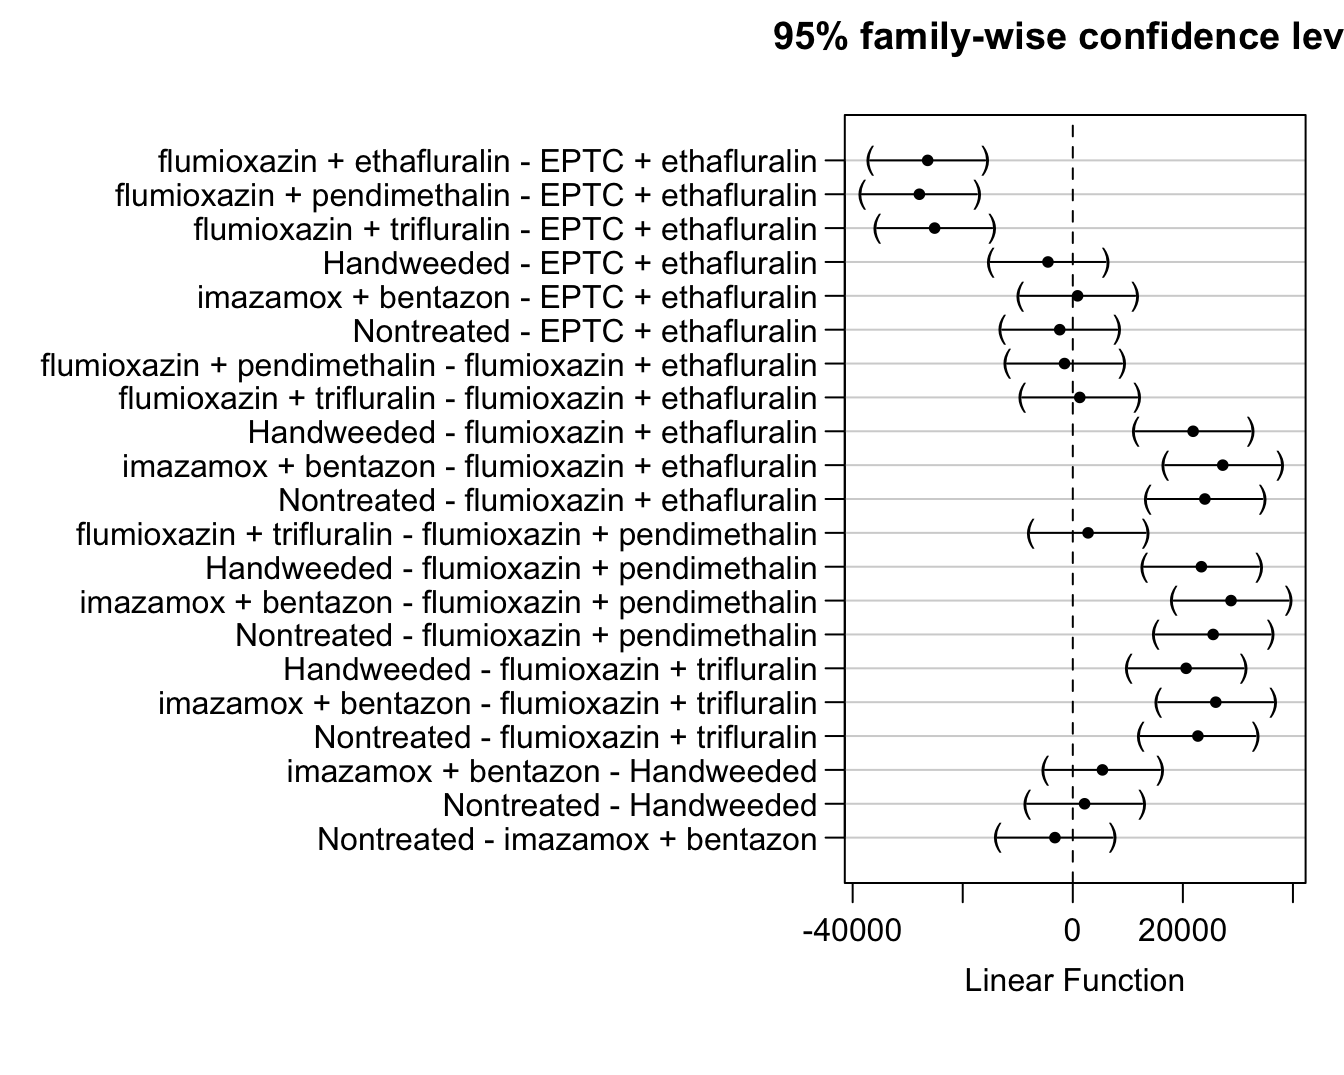
\includegraphics{Rstats4ag_files/figure-latex/figmixedglht-1.pdf}
\caption{\label{fig:figmixedglht}\emph{Model estimates of treatment differences with 95\% confidence intervals.}}
\end{figure}

The \texttt{glht()} function will not allow for unadjusted comparisons, since multiple testing tends to inflate the likelihood of a Type I error. If for some reason unadjusted Fisher LSD p-values are required (similar to the default in SAS) the \texttt{emmeans()} function in the \texttt{emmeans} package can be used. The estimated mrginal means (or least-square means) cna be printed along with the mean separation groups using the \texttt{cld()} function from the \texttt{multcomp} package, and the pairwise comparisons of estimated marginal means can be printed by calling the `contrasts' of the estimated marginal means.

\begin{Shaded}
\begin{Highlighting}[]
\KeywordTok{library}\NormalTok{(emmeans)}
\KeywordTok{emmeans}\NormalTok{(flum.lmer, pairwise }\OperatorTok{~}\StringTok{ }\NormalTok{treatment, }\DataTypeTok{data=}\NormalTok{flum.dat, }\DataTypeTok{adjust=}\StringTok{"none"}\NormalTok{) ->}\StringTok{ }\NormalTok{flum.emm}
\NormalTok{multcomp}\OperatorTok{::}\KeywordTok{cld}\NormalTok{(flum.emm}\OperatorTok{$}\NormalTok{emmeans) }
\end{Highlighting}
\end{Shaded}

\begin{verbatim}
##  treatment                   emmean   SE   df lower.CL upper.CL .group
##  flumioxazin + pendimethalin  20003 3483 20.9    12757    27250  1    
##  flumioxazin + ethafluralin   21508 3483 20.9    14262    28754  1    
##  flumioxazin + trifluralin    22775 3483 20.9    15529    30022  1    
##  Handweeded                   43368 3483 20.9    36122    50614   2   
##  Nontreated                   45506 3483 20.9    38260    52752   2   
##  EPTC + ethafluralin          47882 3483 20.9    40636    55128   2   
##  imazamox + bentazon          48753 3483 20.9    41507    55999   2   
## 
## Degrees-of-freedom method: kenward-roger 
## Confidence level used: 0.95 
## P value adjustment: tukey method for comparing a family of 7 estimates 
## significance level used: alpha = 0.05
\end{verbatim}

\begin{Shaded}
\begin{Highlighting}[]
\NormalTok{flum.emm}\OperatorTok{$}\NormalTok{contrasts}
\end{Highlighting}
\end{Shaded}

\begin{verbatim}
##  contrast                                                 estimate   SE   df t.ratio p.value
##  EPTC + ethafluralin - flumioxazin + ethafluralin            26374 3698 71.1  7.132  <.0001 
##  EPTC + ethafluralin - flumioxazin + pendimethalin           27879 3698 71.1  7.539  <.0001 
##  EPTC + ethafluralin - flumioxazin + trifluralin             25107 3698 71.1  6.790  <.0001 
##  EPTC + ethafluralin - Handweeded                             4514 3698 71.1  1.221  0.2262 
##  EPTC + ethafluralin - imazamox + bentazon                    -871 3698 71.1 -0.236  0.8144 
##  EPTC + ethafluralin - Nontreated                             2376 3698 71.1  0.643  0.5226 
##  flumioxazin + ethafluralin - flumioxazin + pendimethalin     1505 3698 71.1  0.407  0.6853 
##  flumioxazin + ethafluralin - flumioxazin + trifluralin      -1267 3698 71.1 -0.343  0.7328 
##  flumioxazin + ethafluralin - Handweeded                    -21859 3698 71.1 -5.911  <.0001 
##  flumioxazin + ethafluralin - imazamox + bentazon           -27245 3698 71.1 -7.368  <.0001 
##  flumioxazin + ethafluralin - Nontreated                    -23998 3698 71.1 -6.490  <.0001 
##  flumioxazin + pendimethalin - flumioxazin + trifluralin     -2772 3698 71.1 -0.750  0.4559 
##  flumioxazin + pendimethalin - Handweeded                   -23364 3698 71.1 -6.318  <.0001 
##  flumioxazin + pendimethalin - imazamox + bentazon          -28750 3698 71.1 -7.775  <.0001 
##  flumioxazin + pendimethalin - Nontreated                   -25503 3698 71.1 -6.897  <.0001 
##  flumioxazin + trifluralin - Handweeded                     -20592 3698 71.1 -5.569  <.0001 
##  flumioxazin + trifluralin - imazamox + bentazon            -25978 3698 71.1 -7.025  <.0001 
##  flumioxazin + trifluralin - Nontreated                     -22731 3698 71.1 -6.147  <.0001 
##  Handweeded - imazamox + bentazon                            -5386 3698 71.1 -1.456  0.1497 
##  Handweeded - Nontreated                                     -2138 3698 71.1 -0.578  0.5649 
##  imazamox + bentazon - Nontreated                             3247 3698 71.1  0.878  0.3828 
## 
## Degrees-of-freedom method: kenward-roger
\end{verbatim}

\begin{center}\rule{0.5\linewidth}{0.5pt}\end{center}

\hypertarget{mixed-models---regression}{%
\chapter{Mixed Models - Regression}\label{mixed-models---regression}}

\hypertarget{regression-models-with-mixed-effects}{%
\section{Regression Models with Mixed Effects}\label{regression-models-with-mixed-effects}}

When we conduct experiments over several years and/or at several locations, we have to decide if differences among years and/or differences among locations are of interest. In other words: are they fixed effects like the treatments we apply or we want to classify them random effects? If locations are picked at random it seems obvious to define locations as random effects. It means that the location contributes to the variation of the response that cannot be controlled. If the locations are picked according to their weed flora, soil type, and crop pattern, it would be wise to define locations as a fixed effect. Usually, one should use one's common sense and the knowledge of the experimental design and the objectivewhen determining whether locations are fixed or random. There is ongoing discussions among statisticians about what should be random and what should be fixed; but that discussion is somewhat outside this course.

\hypertarget{mixedregressionex1}{%
\subsection{Example 1: Sugarbeet yield}\label{mixedregressionex1}}

Within the many years that sugarbeet has been an economic crop, we incidentally did field experiments in 2006 and 2007, near Powell, Wyoming to determine the effects of duration of Salvia reflexa (lanceleaf sage) interference with sugarbeet (\href{http://www.bioone.org/doi/abs/10.1614/WT-D-10-00015.1}{Odero et al.~2010}). The experiment is also used in the ANCOVA chapter.

\begin{Shaded}
\begin{Highlighting}[]
\NormalTok{lanceleaf.sage<-}\KeywordTok{read.csv}\NormalTok{(}\StringTok{"http://rstats4ag.org/data/lanceleafsage.csv"}\NormalTok{)}
\KeywordTok{head}\NormalTok{(lanceleaf.sage,}\DataTypeTok{n=}\DecValTok{3}\NormalTok{)}
\end{Highlighting}
\end{Shaded}

\begin{verbatim}
##   Replicate Duration Year Yield_Mg.ha Yield.loss.pct
## 1         1       36 2006       67.26          98.05
## 2         1       50 2006       60.34          87.96
## 3         1       64 2006       53.69          78.27
\end{verbatim}

``

First of all we look at the distribution of data within years in Figure \ref{fig:figpanelmreg}:



\begin{Shaded}
\begin{Highlighting}[]
\KeywordTok{library}\NormalTok{(lattice)}
\KeywordTok{xyplot}\NormalTok{(Yield_Mg.ha }\OperatorTok{~}\StringTok{ }\NormalTok{Duration }\OperatorTok{|}\StringTok{ }\KeywordTok{factor}\NormalTok{(Year), }\DataTypeTok{data =}\NormalTok{ lanceleaf.sage,}
    \DataTypeTok{xlab=}\StringTok{"Duration of Competition"}\NormalTok{,}
       \DataTypeTok{panel =} \ControlFlowTok{function}\NormalTok{(x,y)}
\NormalTok{         \{}\KeywordTok{panel.xyplot}\NormalTok{(x,y)}
          \KeywordTok{panel.lmline}\NormalTok{(x,y)\})}
\end{Highlighting}
\end{Shaded}

\begin{figure}
\centering
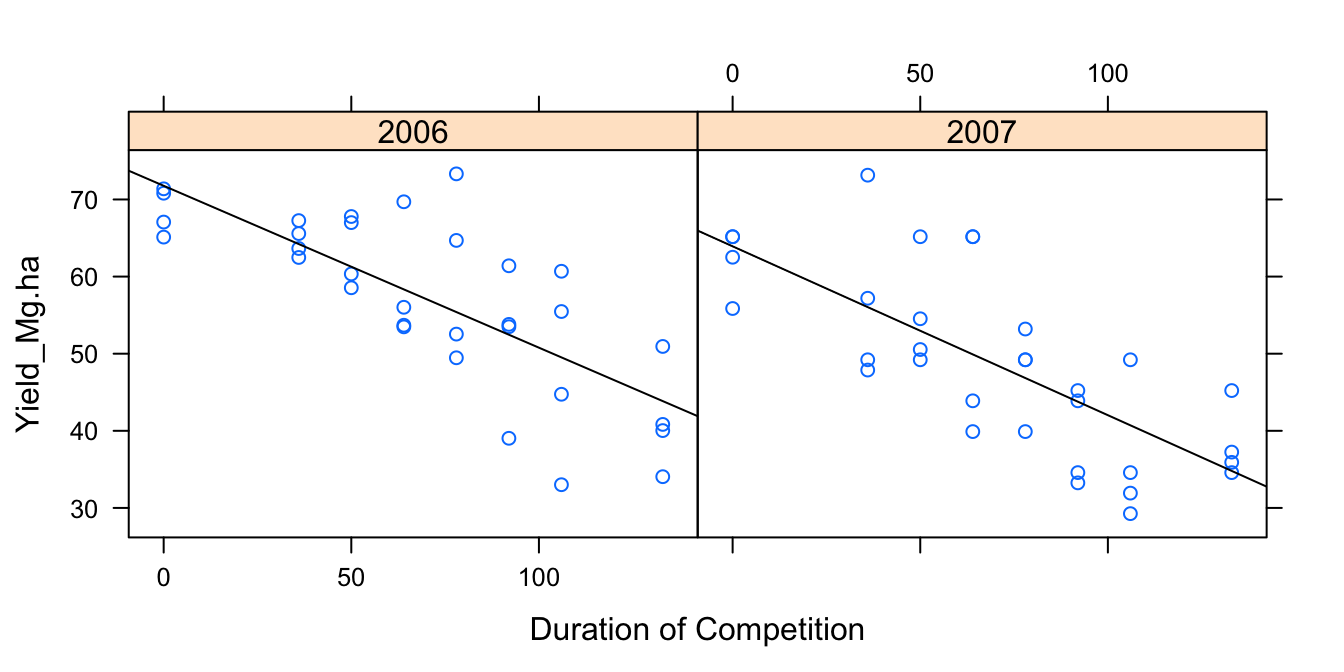
\includegraphics{Rstats4ag_files/figure-latex/figpanelmreg-1.pdf}
\caption{\label{fig:figpanelmreg}\emph{The effect of the duration of weed competition on sugarbeet yield in two different years. It looks as if the relationships could be linear.}}
\end{figure}

The ANCOVA chapter analysis showed a linear regression was acceptable by checking the regression against the most general ANOVA model. The ANCOVA also showed that the regression slopes were the same independent of years, but the intercepts differed between years. In this chapter we now assume that the variation between years are random, because we cannot control the climate.

To analyze this we need to use the \texttt{lmer()}function in the package \texttt{lme4}. The syntax for \texttt{lmer()}is almost the same as for \texttt{lm()}, but there are some limitations and some important additional arguments. In \texttt{lm()} we can convert a continuous x-variable to a factor just by writing \texttt{factor(x)}. You can also do that with fixed effects in the \texttt{lmer()}function, but when it comes to random effects you cannot. In this particular experiment, there are two random effects: experimental years \texttt{(1\textbar{}Year)} and Replicate because it is a block experiment. But the Replicate 1 in year 2006 is not the same as Replicate 1 in 2007. Consequently, we have to make the names for Replicates unambiguously defined with a unique name, so we get a total of 8 unique levels for Year and Replicate combination and the random effect takes the form \texttt{(1\textbar{}New.Rep)} by defining \texttt{New.Rep} using the \texttt{with()} function.

\begin{Shaded}
\begin{Highlighting}[]
\NormalTok{lanceleaf.sage}\OperatorTok{$}\NormalTok{New.Rep <-}\StringTok{ }\KeywordTok{with}\NormalTok{(lanceleaf.sage, }\KeywordTok{factor}\NormalTok{(Replicate)}\OperatorTok{:}\KeywordTok{factor}\NormalTok{(Year))}
\KeywordTok{levels}\NormalTok{(lanceleaf.sage}\OperatorTok{$}\NormalTok{New.Rep)}
\end{Highlighting}
\end{Shaded}

\begin{verbatim}
## [1] "1:2006" "1:2007" "2:2006" "2:2007" "3:2006" "3:2007" "4:2006" "4:2007"
\end{verbatim}

After this initial exercise, we are now ready to test whether we can assume linearity of Yield on duration of competition. We compare the regression model with the most general model, the ANOVA, as it is becoming standard practice in the course.

\begin{Shaded}
\begin{Highlighting}[]
\KeywordTok{library}\NormalTok{(lme4)}
\NormalTok{Anova.m1 <-}\StringTok{ }\KeywordTok{lmer}\NormalTok{(Yield_Mg.ha }\OperatorTok{~}\StringTok{ }\KeywordTok{factor}\NormalTok{(Duration) }\OperatorTok{+}\StringTok{ }\NormalTok{(}\DecValTok{1}\OperatorTok{|}\NormalTok{Year) }\OperatorTok{+}\StringTok{ }\NormalTok{(}\DecValTok{1}\OperatorTok{|}\NormalTok{New.Rep),}
                 \DataTypeTok{data=}\NormalTok{lanceleaf.sage, }\DataTypeTok{REML=}\OtherTok{FALSE}\NormalTok{)}
\NormalTok{Regression.m2 <-}\StringTok{ }\KeywordTok{lmer}\NormalTok{(Yield_Mg.ha }\OperatorTok{~}\StringTok{ }\NormalTok{Duration }\OperatorTok{+}\StringTok{ }\NormalTok{(}\DecValTok{1}\OperatorTok{|}\NormalTok{Year) }\OperatorTok{+}\StringTok{ }\NormalTok{(}\DecValTok{1}\OperatorTok{|}\NormalTok{New.Rep),}
                      \DataTypeTok{data=}\NormalTok{lanceleaf.sage, }\DataTypeTok{REML=}\OtherTok{FALSE}\NormalTok{)}
\KeywordTok{anova}\NormalTok{(Anova.m1, Regression.m2) }\CommentTok{#No indication of nonlinearity}
\end{Highlighting}
\end{Shaded}

\begin{verbatim}
## Data: lanceleaf.sage
## Models:
## Regression.m2: Yield_Mg.ha ~ Duration + (1 | Year) + (1 | New.Rep)
## Anova.m1: Yield_Mg.ha ~ factor(Duration) + (1 | Year) + (1 | New.Rep)
##               npar    AIC    BIC  logLik deviance Chisq Df Pr(>Chisq)
## Regression.m2    5 454.77 465.56 -222.38   444.77                    
## Anova.m1        11 460.97 484.72 -219.49   438.97 5.791  6      0.447
\end{verbatim}

The test for lack of fit is non-significant as was also seen in the ANCOVA chapter.

Notice, we have an argument that is not used in the general \texttt{lm()} and it is \texttt{REML} (Rstricted Maximum Likelihood). There are two options: Maximum Likelihood estimation (ML) REML. \texttt{REML=TRUE} is the default. ML produces downwards biased estimated variance components (over-optimistic precision). REML reduces the bias (similar to dividing by n - p rather than n for the residual standard error in linear regression). In other words REML agrees with \texttt{lm()} in case of no random effects. To make a long story short, we should use ML (\texttt{REML=FALSE}) when comparing models using the \texttt{anova()} function.

However, when we look at the summary of the mixed effect regression:

\begin{Shaded}
\begin{Highlighting}[]
\KeywordTok{summary}\NormalTok{(Regression.m2)}
\end{Highlighting}
\end{Shaded}

\begin{verbatim}
## Linear mixed model fit by maximum likelihood  ['lmerMod']
## Formula: Yield_Mg.ha ~ Duration + (1 | Year) + (1 | New.Rep)
##    Data: lanceleaf.sage
## 
##      AIC      BIC   logLik deviance df.resid 
##    454.8    465.6   -222.4    444.8       59 
## 
## Scaled residuals: 
##      Min       1Q   Median       3Q      Max 
## -1.71954 -0.65323 -0.09755  0.53285  2.36798 
## 
## Random effects:
##  Groups   Name        Variance Std.Dev.
##  New.Rep  (Intercept)  8.993   2.999   
##  Year     (Intercept) 14.092   3.754   
##  Residual             52.217   7.226   
## Number of obs: 64, groups:  New.Rep, 8; Year, 2
## 
## Fixed effects:
##             Estimate Std. Error t value
## (Intercept) 67.85642    3.40236  19.944
## Duration    -0.21451    0.02303  -9.314
## 
## Correlation of Fixed Effects:
##          (Intr)
## Duration -0.473
\end{verbatim}

it looks rather different from an ordinary regression summary with the \texttt{lm()} function. The first thing we see is that there are no significance levels like in \texttt{lm()} output. This is because there is still no consensus about how to calculate degrees of freedom for mixed effects models. There is fairly extensive discussion of this topic in the R community, that can be left out here, but we will point you to a breif explanation provided by \href{https://stat.ethz.ch/pipermail/r-help/2006-May/094765.html}{Douglas Bates}, the author of the \texttt{lmer()} function.

Variation between years (Year) and variation between reps within year (New.Rep) are both provided in the random effects portion of the output. What it means is that the variance between years and the variation among Replicates cannot be controlled by us; therefore we define them as random effect and they are now an integral part of the total variation we cannot explain.

Comparing the result above with the fixed year effect:

\begin{Shaded}
\begin{Highlighting}[]
\NormalTok{regression.fixed<-}\KeywordTok{lm}\NormalTok{(Yield_Mg.ha }\OperatorTok{~}\StringTok{ }\NormalTok{Duration }\OperatorTok{+}\StringTok{ }\KeywordTok{factor}\NormalTok{(Year), }\DataTypeTok{data=}\NormalTok{lanceleaf.sage)}
\KeywordTok{summary}\NormalTok{(regression.fixed)}
\end{Highlighting}
\end{Shaded}

\begin{verbatim}
## 
## Call:
## lm(formula = Yield_Mg.ha ~ Duration + factor(Year), data = lanceleaf.sage)
## 
## Residuals:
##      Min       1Q   Median       3Q      Max 
## -16.3477  -5.2428  -0.7246   3.5724  17.9560 
## 
## Coefficients:
##                  Estimate Std. Error t value Pr(>|t|)    
## (Intercept)      72.09580    2.20523  32.693  < 2e-16 ***
## Duration         -0.21451    0.02472  -8.678 3.02e-12 ***
## factor(Year)2007 -8.47875    1.93890  -4.373 4.86e-05 ***
## ---
## Signif. codes:  0 '***' 0.001 '**' 0.01 '*' 0.05 '.' 0.1 ' ' 1
## 
## Residual standard error: 7.756 on 61 degrees of freedom
## Multiple R-squared:  0.6075, Adjusted R-squared:  0.5947 
## F-statistic: 47.21 on 2 and 61 DF,  p-value: 4.081e-13
\end{verbatim}

We see that the slope for the mixed model is the same as for the fixed year model -0.21 with standard error of 0.02. The intercept of the mixed model is 67.9 (3.4). For the fixed effect model the intercepts were 72.1 and 72.1 -8.5 = 63.6with a standard error of 2.2 and 1.9, respectively. The changes of going from fixed year effect to random year effect is not dramatic when it comes to regression slopes, either. But if we decide year is random, then the mixed model is the one to use. We get a bonus, however by separating the variation of years from the residual. Reporting this information gives others who want to include our results in a meta-analysis knowledge of the actual variation in the experiments.

The illustration of the results is shown below. In order to make the plot neat we take the averages of the measurements by using the package \texttt{dplyr}, before plotting the data in Figure \ref{fig:figmregresults}.



\begin{Shaded}
\begin{Highlighting}[]
\KeywordTok{library}\NormalTok{(dplyr)}
\NormalTok{averages<-lanceleaf.sage }\OperatorTok
\StringTok{  }\KeywordTok{group_by}\NormalTok{(Duration,Year) }\OperatorTok
\StringTok{  }\KeywordTok{summarise}\NormalTok{(}\DataTypeTok{YIELD =} \KeywordTok{mean}\NormalTok{(Yield_Mg.ha))}
\KeywordTok{par}\NormalTok{(}\DataTypeTok{mar=}\KeywordTok{c}\NormalTok{(}\FloatTok{3.2}\NormalTok{,}\FloatTok{3.2}\NormalTok{,.}\DecValTok{5}\NormalTok{,.}\DecValTok{5}\NormalTok{), }\DataTypeTok{mgp=}\KeywordTok{c}\NormalTok{(}\DecValTok{2}\NormalTok{,.}\DecValTok{7}\NormalTok{,}\DecValTok{0}\NormalTok{))}
\KeywordTok{plot}\NormalTok{(YIELD }\OperatorTok{~}\StringTok{ }\NormalTok{Duration, }\DataTypeTok{data =}\NormalTok{ averages, }\DataTypeTok{bty=}\StringTok{"l"}\NormalTok{,}
     \DataTypeTok{ylab =} \KeywordTok{quote}\NormalTok{(Yield}\OperatorTok{~}\NormalTok{(kg}\OperatorTok{~}\NormalTok{ha}\OperatorTok{^-}\DecValTok{1}\NormalTok{)), }\CommentTok{#Note how to use dimension accepted in some journals}
     \DataTypeTok{xlab =} \StringTok{"Duration of competition"}\NormalTok{,}
     \DataTypeTok{pch  =} \KeywordTok{as.numeric}\NormalTok{(}\KeywordTok{factor}\NormalTok{(Year)), }\DataTypeTok{ylim=}\KeywordTok{c}\NormalTok{(}\DecValTok{10}\NormalTok{,}\DecValTok{80}\NormalTok{))}
  \KeywordTok{abline}\NormalTok{(}\KeywordTok{fixef}\NormalTok{(Regression.m2))}
\end{Highlighting}
\end{Shaded}

\begin{figure}
\centering
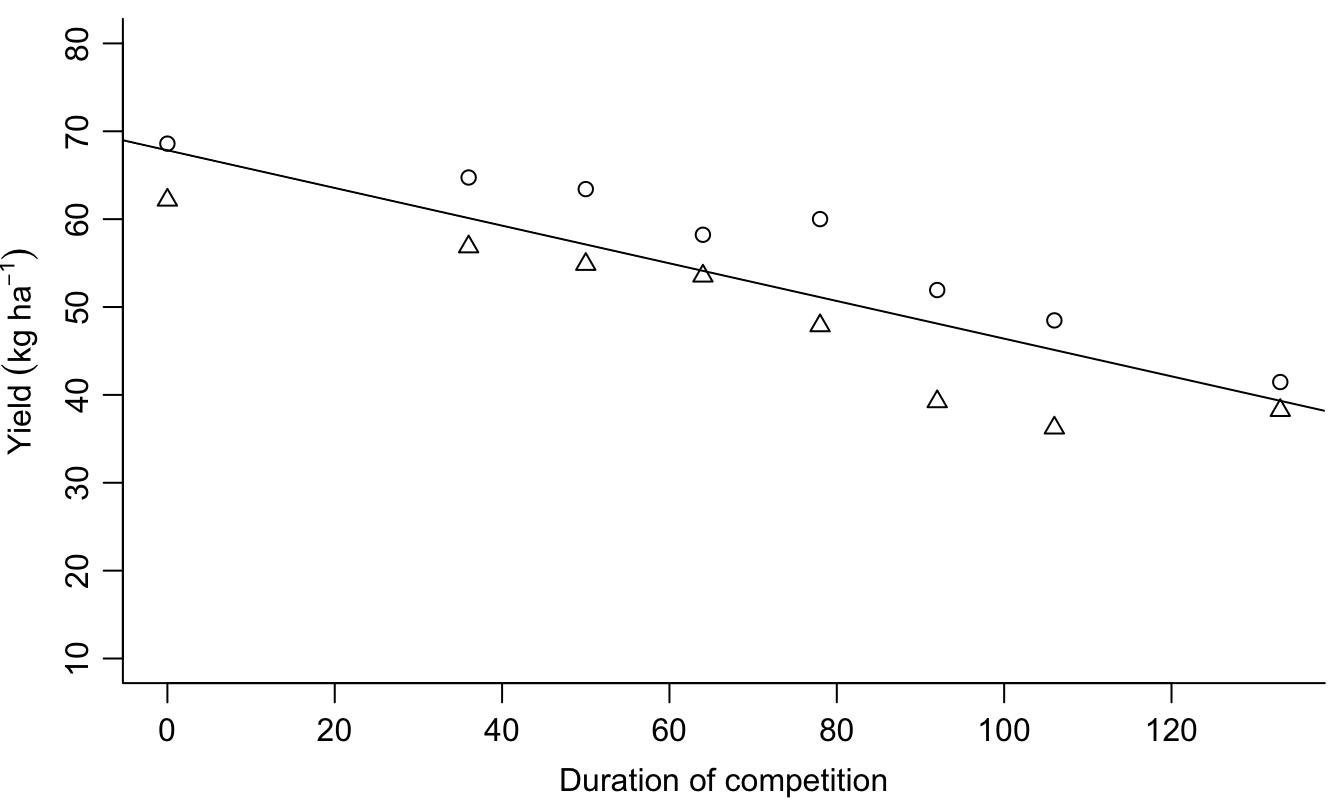
\includegraphics{Rstats4ag_files/figure-latex/figmregresults-1.pdf}
\caption{\label{fig:figmregresults}\emph{The regression model with year as a random effect. Note that in this instance we have one slope and one intercept, and the regression line now is almost in the middle. Note that the \texttt{fixef(Regression.m2)} contains the fixed regressions parameters and the ordinary \texttt{abline()} can be used.}}
\end{figure}

\hypertarget{example-2-fungicide-toxicity}{%
\subsection{Example 2: Fungicide toxicity}\label{example-2-fungicide-toxicity}}

Another example is with a total of six concentration-response experiments evaluating
the effect of a fungicide, vinclozolin on luminescence of ovary cells. Vinclozolin is a putative endogenous disruptor and therefore banned in Denmark. The concentration-response curves were run on separate days and it shows that the calibration of the instrument makes the response-curves somewhat different.

\begin{Shaded}
\begin{Highlighting}[]
\NormalTok{vinclozolin <-}\StringTok{ }\KeywordTok{read.csv}\NormalTok{(}\StringTok{"http://rstats4ag.org/data/vinclozolin.csv"}\NormalTok{)}
\KeywordTok{head}\NormalTok{(vinclozolin)}
\end{Highlighting}
\end{Shaded}

\begin{verbatim}
##    conc effect experiment
## 1 0.025    908      10509
## 2 0.050    997      10509
## 3 0.100    744      10509
## 4 0.200    567      10509
## 5 0.390    314      10509
## 6 0.780    325      10509
\end{verbatim}

Figure \ref{fig:figfungpanel} shows the individual response curves illustrating the variation in the slope and intercept of the straight lines. However, the variation is kind of erratic because of daily calibration of the machine. Therefore, we consider days a random effect, the variation is intangible. As was the case with the duration of competition we will change the numeric name of each experiment to a factor:

\begin{Shaded}
\begin{Highlighting}[]
\NormalTok{vinclozolin}\OperatorTok{$}\NormalTok{Experiment <-}\StringTok{ }\KeywordTok{factor}\NormalTok{(vinclozolin}\OperatorTok{$}\NormalTok{experiment)}
\end{Highlighting}
\end{Shaded}

And then run the analysis, but first we illustrate thevariation in data (Figure \ref{fig:figfungpanel}).



\begin{Shaded}
\begin{Highlighting}[]
\KeywordTok{library}\NormalTok{(lattice)}
\KeywordTok{xyplot}\NormalTok{(effect }\OperatorTok{~}\StringTok{ }\KeywordTok{log}\NormalTok{(conc) }\OperatorTok{|}\StringTok{ }\NormalTok{Experiment, }\DataTypeTok{data =}\NormalTok{ vinclozolin,}
       \DataTypeTok{xlab =} \StringTok{"Log( Concentration of Vinclozolin)"}\NormalTok{, }\DataTypeTok{ylab =} \StringTok{"Luminescence"}\NormalTok{,}
       \DataTypeTok{panel =} \ControlFlowTok{function}\NormalTok{(x,y)}
\NormalTok{         \{}\KeywordTok{panel.xyplot}\NormalTok{(x,y)}
          \KeywordTok{panel.lmline}\NormalTok{(x,y)\})}
\end{Highlighting}
\end{Shaded}

\begin{figure}
\centering
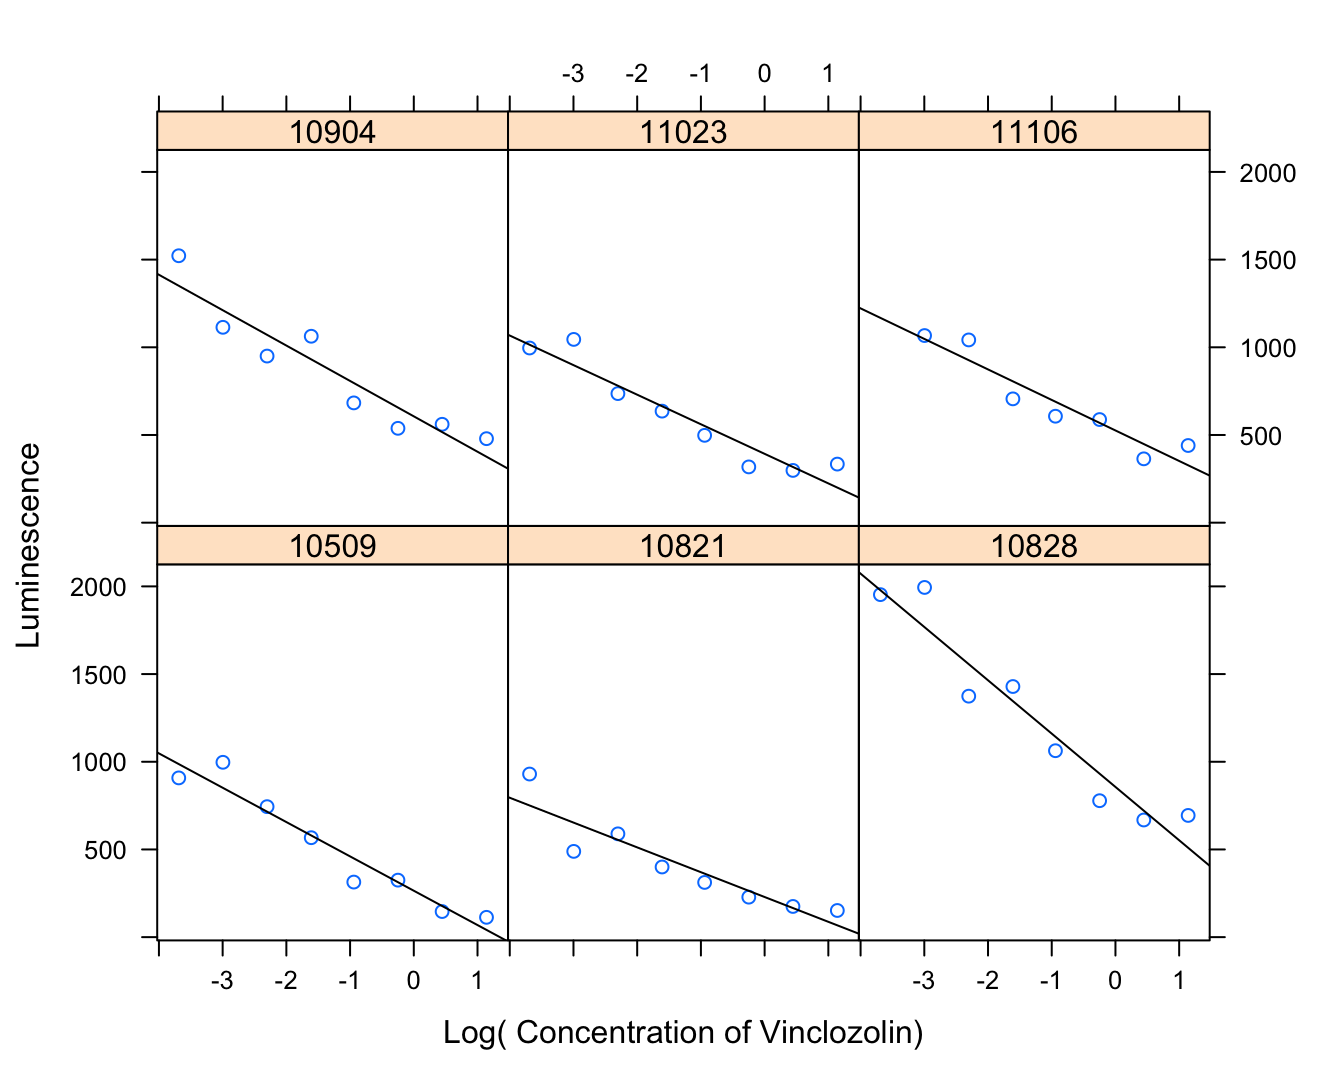
\includegraphics{Rstats4ag_files/figure-latex/figfungpanel-1.pdf}
\caption{\label{fig:figfungpanel}\emph{Concentration-response curves for ovary cell luminescence on venclozolin.}}
\end{figure}

The procedure to run the mixed regression model is the same as for \protect\hyperlink{mixedregressionex1}{the sugarbeet example}. First we conduct a lack-of-fit test against the most general model - ANOVA.

\begin{Shaded}
\begin{Highlighting}[]
\KeywordTok{library}\NormalTok{(lme4)}
\NormalTok{vinclo.mixed.ANOVA <-}\StringTok{ }\KeywordTok{lmer}\NormalTok{(effect }\OperatorTok{~}\StringTok{ }\KeywordTok{factor}\NormalTok{(conc) }\OperatorTok{+}\StringTok{ }\NormalTok{(}\DecValTok{1}\OperatorTok{|}\NormalTok{Experiment),}
                           \DataTypeTok{data =}\NormalTok{ vinclozolin, }\DataTypeTok{REML =} \OtherTok{FALSE}\NormalTok{)}
\NormalTok{vinclo.mixed.Regression <-}\StringTok{ }\KeywordTok{lmer}\NormalTok{(effect }\OperatorTok{~}\StringTok{ }\KeywordTok{log}\NormalTok{(conc) }\OperatorTok{+}\StringTok{ }\NormalTok{(}\DecValTok{1}\OperatorTok{|}\NormalTok{Experiment),}
                                \DataTypeTok{data =}\NormalTok{ vinclozolin, }\DataTypeTok{REML =} \OtherTok{FALSE}\NormalTok{)}
\KeywordTok{anova}\NormalTok{(vinclo.mixed.ANOVA, vinclo.mixed.Regression)}
\end{Highlighting}
\end{Shaded}

\begin{verbatim}
## Data: vinclozolin
## Models:
## vinclo.mixed.Regression: effect ~ log(conc) + (1 | Experiment)
## vinclo.mixed.ANOVA: effect ~ factor(conc) + (1 | Experiment)
##                         npar    AIC    BIC  logLik deviance Chisq Df Pr(>Chisq)
## vinclo.mixed.Regression    4 627.06 634.46 -309.53   619.06                    
## vinclo.mixed.ANOVA        10 628.42 646.92 -304.21   608.42 10.64  6     0.1002
\end{verbatim}

The test for lack of fit is non-significant so we can assume the relationship is linear, whatever the day. Please note that we only have one replication per regression per day. But the concentrations are the same, so a test for lack of fit is still appropriate.

\begin{Shaded}
\begin{Highlighting}[]
\KeywordTok{summary}\NormalTok{(vinclo.mixed.Regression)}
\end{Highlighting}
\end{Shaded}

\begin{verbatim}
## Linear mixed model fit by maximum likelihood  ['lmerMod']
## Formula: effect ~ log(conc) + (1 | Experiment)
##    Data: vinclozolin
## 
##      AIC      BIC   logLik deviance df.resid 
##    627.1    634.5   -309.5    619.1       43 
## 
## Scaled residuals: 
##     Min      1Q  Median      3Q     Max 
## -1.9356 -0.6270 -0.2354  0.6112  3.0031 
## 
## Random effects:
##  Groups     Name        Variance Std.Dev.
##  Experiment (Intercept) 72092    268.5   
##  Residual               19987    141.4   
## Number of obs: 47, groups:  Experiment, 6
## 
## Fixed effects:
##             Estimate Std. Error t value
## (Intercept)   478.77     112.71   4.248
## log(conc)    -199.03      13.31 -14.956
## 
## Correlation of Fixed Effects:
##           (Intr)
## log(conc) 0.144
\end{verbatim}

The variation among experimental days (268) is huge compared with the variation within days (141).



\begin{Shaded}
\begin{Highlighting}[]
\KeywordTok{xyplot}\NormalTok{(effect}\OperatorTok{~}\KeywordTok{log}\NormalTok{(conc)}\OperatorTok{|}\NormalTok{experiment, }\DataTypeTok{data=}\NormalTok{vinclozolin,}
       \DataTypeTok{xlab=}\StringTok{"Log( Concentration of Vinclozolin)"}\NormalTok{, }\DataTypeTok{ylab=}\StringTok{"Luminescence"}\NormalTok{,}
       \DataTypeTok{panel=}\ControlFlowTok{function}\NormalTok{(...)}
\NormalTok{         \{}\KeywordTok{panel.xyplot}\NormalTok{(...);}
          \KeywordTok{panel.abline}\NormalTok{(}\KeywordTok{fixef}\NormalTok{(vinclo.mixed.Regression))\})}
\end{Highlighting}
\end{Shaded}

\begin{figure}
\centering
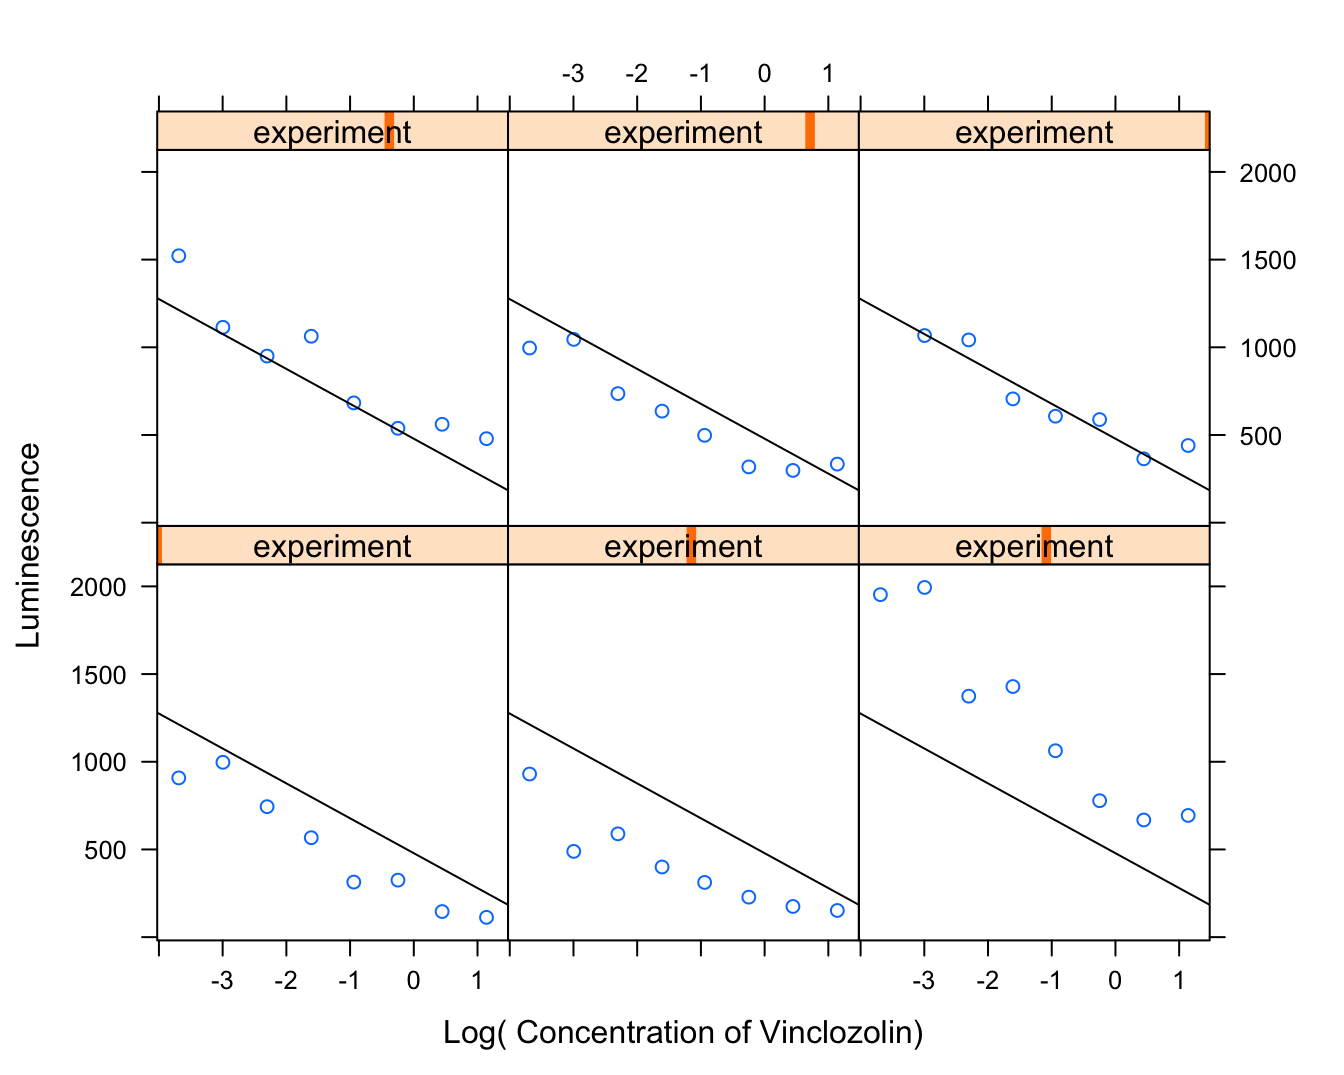
\includegraphics{Rstats4ag_files/figure-latex/figfungpaneldays-1.pdf}
\caption{\label{fig:figfungpaneldays}\emph{Regression lines for all 6 days shown in six panels to give an idea of the variation among days. There appear to be particularly large differences between the responses and the regression lines for the three days in the lower panels.}}
\end{figure}

If we had run an ordinary regression by pooling the six concentration-response curves then we would have gotten the result below.

\begin{Shaded}
\begin{Highlighting}[]
\NormalTok{vinclo.fixed.Regression<-}\KeywordTok{lm}\NormalTok{(effect }\OperatorTok{~}\StringTok{ }\KeywordTok{log}\NormalTok{(conc), }\DataTypeTok{data =}\NormalTok{ vinclozolin)}
\KeywordTok{summary}\NormalTok{(vinclo.fixed.Regression)}
\end{Highlighting}
\end{Shaded}

\begin{verbatim}
## 
## Call:
## lm(formula = effect ~ log(conc), data = vinclozolin)
## 
## Residuals:
##     Min      1Q  Median      3Q     Max 
## -584.64 -212.74  -58.83  179.01  920.36 
## 
## Coefficients:
##             Estimate Std. Error t value Pr(>|t|)    
## (Intercept)   478.90      58.03   8.253 1.48e-10 ***
## log(conc)    -198.53      29.33  -6.768 2.25e-08 ***
## ---
## Signif. codes:  0 '***' 0.001 '**' 0.01 '*' 0.05 '.' 0.1 ' ' 1
## 
## Residual standard error: 312.6 on 45 degrees of freedom
## Multiple R-squared:  0.5044, Adjusted R-squared:  0.4934 
## F-statistic:  45.8 on 1 and 45 DF,  p-value: 2.253e-08
\end{verbatim}

The slope and the intercept are almost identical for the two \texttt{lmer()}and \texttt{lm()}. The standard errors for the intercept, though, roughly doubled, 58 for \texttt{lm()} to 113 for \texttt{lmer()}, whereas the slope was more that halved, 13, for the \texttt{lmer()}compared to 29 with \texttt{lm()}. Undoubtedly, the experimental dates improved the precision of the slope. We can compare the fixed and random effects models on these data using Akaike Information Criterion (AIC). For a given set of data, the model with the lowest AIC value is more likely to be the appropriate model.

\begin{Shaded}
\begin{Highlighting}[]
\KeywordTok{AIC}\NormalTok{(vinclo.mixed.Regression, vinclo.fixed.Regression)}
\end{Highlighting}
\end{Shaded}

\begin{verbatim}
##                         df      AIC
## vinclo.mixed.Regression  4 627.0628
## vinclo.fixed.Regression  3 677.3501
\end{verbatim}

As a gereral rule, differences in AIC values less than 10 indicate two models perform similarly in describing the data. For the vinclozolin data set, the mixed model has and AIC of 627 compared to 677 for the fixed model where the effect of day was not included. This indicates the mixed model is the best fit for these data.

\begin{center}\rule{0.5\linewidth}{0.5pt}\end{center}

\hypertarget{logistic-regression-binary-response}{%
\chapter{Logistic Regression (Binary Response)}\label{logistic-regression-binary-response}}

Determination of the effective dose of a herbicide under field, greenhouse, or laboratory conditions is a common goal of weed science experiments. Although the response variable in some cases is continuous (dry weight) or percent (visual injury), in many cases the response variable of interest is a binary response, such as mortality (the plant is alive or dead). This type of data is important in many types of toxicology and pest management, and weed science is no exception. In many ways the analysis of binary response data is analogous to using ANOVA followed by non-linear regression.

\hypertarget{generalized-linear-model}{%
\section{Generalized Linear Model}\label{generalized-linear-model}}

Instead of fitting a linear model using the lm() function, analysis of binary response data requires the use of a generalized linear model with the glm() function. For this example, the data set has mortality observations collected 21 days after treatment with six rates of imazamox with and without six different growth regulator herbicides.

\begin{Shaded}
\begin{Highlighting}[]
\NormalTok{rye.dat <-}\StringTok{ }\KeywordTok{read.csv}\NormalTok{(}\StringTok{"http://rstats4ag.org/data/2012_RyeGH.csv"}\NormalTok{)}
\NormalTok{rye.glm <-}\StringTok{ }\KeywordTok{glm}\NormalTok{(mort}\FloatTok{.21}\NormalTok{dat }\OperatorTok{~}\StringTok{ }\NormalTok{imaz.rate }\OperatorTok{+}\StringTok{ }\NormalTok{gr, }\DataTypeTok{data =}\NormalTok{ rye.dat, }
               \DataTypeTok{family =} \KeywordTok{binomial}\NormalTok{(}\DataTypeTok{link =} \StringTok{"logit"}\NormalTok{))}
\KeywordTok{anova}\NormalTok{(rye.glm, }\DataTypeTok{test =} \StringTok{"Chisq"}\NormalTok{)}
\end{Highlighting}
\end{Shaded}

\begin{verbatim}
## Analysis of Deviance Table
## 
## Model: binomial, link: logit
## 
## Response: mort.21dat
## 
## Terms added sequentially (first to last)
## 
## 
##           Df Deviance Resid. Df Resid. Dev  Pr(>Chi)    
## NULL                        430     464.54              
## imaz.rate  1   93.502       429     371.04 < 2.2e-16 ***
## gr         7   31.180       422     339.86 5.759e-05 ***
## ---
## Signif. codes:  0 '***' 0.001 '**' 0.01 '*' 0.05 '.' 0.1 ' ' 1
\end{verbatim}

Using \texttt{anova()} on the \texttt{glm()} fit results in an analysis of deviance table with a similar interpretation as an ANOVA table for continuous response data. Both the imazamox rate and growth regulator herbicide significantly affected the mortality of feral rye, which was the expected result. The drc package can be used to quantify the response of feral rye to imazamox in the presence and absence of the growth regulator herbicides.

\begin{Shaded}
\begin{Highlighting}[]
\KeywordTok{library}\NormalTok{(drc)}
\NormalTok{rye.drc <-}\StringTok{ }\KeywordTok{drm}\NormalTok{(mort}\FloatTok{.21}\NormalTok{dat }\OperatorTok{~}\StringTok{ }\NormalTok{imaz.rate, gr, }\DataTypeTok{data =}\NormalTok{ rye.dat, }\DataTypeTok{fct =} \KeywordTok{LL.2}\NormalTok{(), }
               \DataTypeTok{type =} \StringTok{"binomial"}\NormalTok{, }\DataTypeTok{na.action =}\NormalTok{ na.omit)}
\end{Highlighting}
\end{Shaded}

\begin{verbatim}
## Control measurements detected for level: Control
\end{verbatim}

\begin{Shaded}
\begin{Highlighting}[]
\KeywordTok{summary}\NormalTok{(rye.drc)}
\end{Highlighting}
\end{Shaded}

\begin{verbatim}
## 
## Model fitted: Log-logistic (ED50 as parameter) with lower limit at 0 and upper limit at 1 (2 parms)
## 
## Parameter estimates:
## 
##               Estimate Std. Error t-value   p-value    
## b:None         1.31358    0.52697  2.4927 0.0126766 *  
## b:2,4-D amine  1.93438    0.63004  3.0702 0.0021389 ** 
## b:2,4-D ester  1.83033    0.45369  4.0343 5.476e-05 ***
## b:MCPA amine   2.00705    0.67980  2.9524 0.0031531 ** 
## b:MCPA ester   1.16337    0.34724  3.3503 0.0008071 ***
## b:dicamba      2.38035    0.79232  3.0043 0.0026623 ** 
## b:fluroxypyr   1.93821    0.63093  3.0720 0.0021264 ** 
## e:None        97.74085   48.66554  2.0084 0.0445987 *  
## e:2,4-D amine 61.90448   15.27230  4.0534 5.048e-05 ***
## e:2,4-D ester 25.55234    4.80647  5.3162 1.059e-07 ***
## e:MCPA amine  66.09968   16.64430  3.9713 7.148e-05 ***
## e:MCPA ester  28.58611    7.85012  3.6415 0.0002711 ***
## e:dicamba     62.04112   12.76510  4.8602 1.173e-06 ***
## e:fluroxypyr  61.84463   15.21629  4.0644 4.816e-05 ***
## ---
## Signif. codes:  0 '***' 0.001 '**' 0.01 '*' 0.05 '.' 0.1 ' ' 1
\end{verbatim}

\begin{Shaded}
\begin{Highlighting}[]
\KeywordTok{EDcomp}\NormalTok{(rye.drc, }\KeywordTok{c}\NormalTok{(}\DecValTok{50}\NormalTok{,}\DecValTok{50}\NormalTok{))}
\end{Highlighting}
\end{Shaded}

\begin{verbatim}
## 
## Estimated ratios of effect doses
## 
##                                  Estimate  Std. Error     t-value     p-value
## 2,4-D amine/2,4-D ester:50/50  2.4227e+00  7.5160e-01  1.8928e+00  5.8379e-02
## 2,4-D amine/dicamba:50/50      9.9780e-01  3.2054e-01 -6.8712e-03  9.9452e-01
## 2,4-D amine/fluroxypyr:50/50   1.0010e+00  3.4876e-01  2.7746e-03  9.9779e-01
## 2,4-D amine/MCPA amine:50/50   9.3653e-01  3.3015e-01 -1.9224e-01  8.4755e-01
## 2,4-D amine/MCPA ester:50/50   2.1655e+00  7.9943e-01  1.4580e+00  1.4485e-01
## 2,4-D amine/None:50/50         6.3335e-01  3.5194e-01 -1.0418e+00  2.9751e-01
## 2,4-D ester/dicamba:50/50      4.1186e-01  1.1482e-01 -5.1224e+00  3.0171e-07
## 2,4-D ester/fluroxypyr:50/50   4.1317e-01  1.2796e-01 -4.5860e+00  4.5186e-06
## 2,4-D ester/MCPA amine:50/50   3.8657e-01  1.2150e-01 -5.0487e+00  4.4489e-07
## 2,4-D ester/MCPA ester:50/50   8.9387e-01  2.9753e-01 -3.5669e-01  7.2132e-01
## 2,4-D ester/None:50/50         2.6143e-01  1.3915e-01 -5.3079e+00  1.1091e-07
## dicamba/fluroxypyr:50/50       1.0032e+00  3.2175e-01  9.8746e-03  9.9212e-01
## dicamba/MCPA amine:50/50       9.3860e-01  3.0521e-01 -2.0117e-01  8.4056e-01
## dicamba/MCPA ester:50/50       2.1703e+00  7.4473e-01  1.5715e+00  1.1607e-01
## dicamba/None:50/50             6.3475e-01  3.4197e-01 -1.0681e+00  2.8548e-01
## fluroxypyr/MCPA amine:50/50    9.3563e-01  3.2939e-01 -1.9543e-01  8.4506e-01
## fluroxypyr/MCPA ester:50/50    2.1635e+00  7.9769e-01  1.4585e+00  1.4470e-01
## fluroxypyr/None:50/50          6.3274e-01  3.5141e-01 -1.0451e+00  2.9598e-01
## MCPA amine/MCPA ester:50/50    2.3123e+00  8.6153e-01  1.5232e+00  1.2770e-01
## MCPA amine/None:50/50          6.7627e-01  3.7733e-01 -8.5793e-01  3.9093e-01
## MCPA ester/None:50/50          2.9247e-01  1.6630e-01 -4.2545e+00  2.0950e-05
\end{verbatim}

Please note that the test for significant relative potency is not a null hypothesis, but that the relative potency SI is different from unity.



\begin{Shaded}
\begin{Highlighting}[]
\KeywordTok{par}\NormalTok{(}\DataTypeTok{mar=}\KeywordTok{c}\NormalTok{(}\FloatTok{3.2}\NormalTok{,}\FloatTok{3.2}\NormalTok{,.}\DecValTok{5}\NormalTok{,.}\DecValTok{5}\NormalTok{), }\DataTypeTok{mgp=}\KeywordTok{c}\NormalTok{(}\DecValTok{2}\NormalTok{,.}\DecValTok{7}\NormalTok{,}\DecValTok{0}\NormalTok{))}
\KeywordTok{plot}\NormalTok{(rye.drc, }\DataTypeTok{legendPos=}\KeywordTok{c}\NormalTok{(}\DecValTok{10}\NormalTok{,}\FloatTok{0.6}\NormalTok{), }\DataTypeTok{col=}\NormalTok{T, }\DataTypeTok{xt=}\KeywordTok{unique}\NormalTok{(rye.dat}\OperatorTok{$}\NormalTok{imaz.rate),}
     \DataTypeTok{broken=}\NormalTok{T, }\DataTypeTok{bp=}\FloatTok{1.5}\NormalTok{, }\DataTypeTok{xlim=}\KeywordTok{c}\NormalTok{(}\DecValTok{0}\NormalTok{,}\DecValTok{100}\NormalTok{),}\DataTypeTok{xlab=}\StringTok{"Imazamox rate"}\NormalTok{, }\DataTypeTok{bty=}\StringTok{"l"}\NormalTok{,}
     \DataTypeTok{ylab=}\StringTok{"Probability of survival 21 DAT"}\NormalTok{)}
\end{Highlighting}
\end{Shaded}

\begin{figure}
\centering
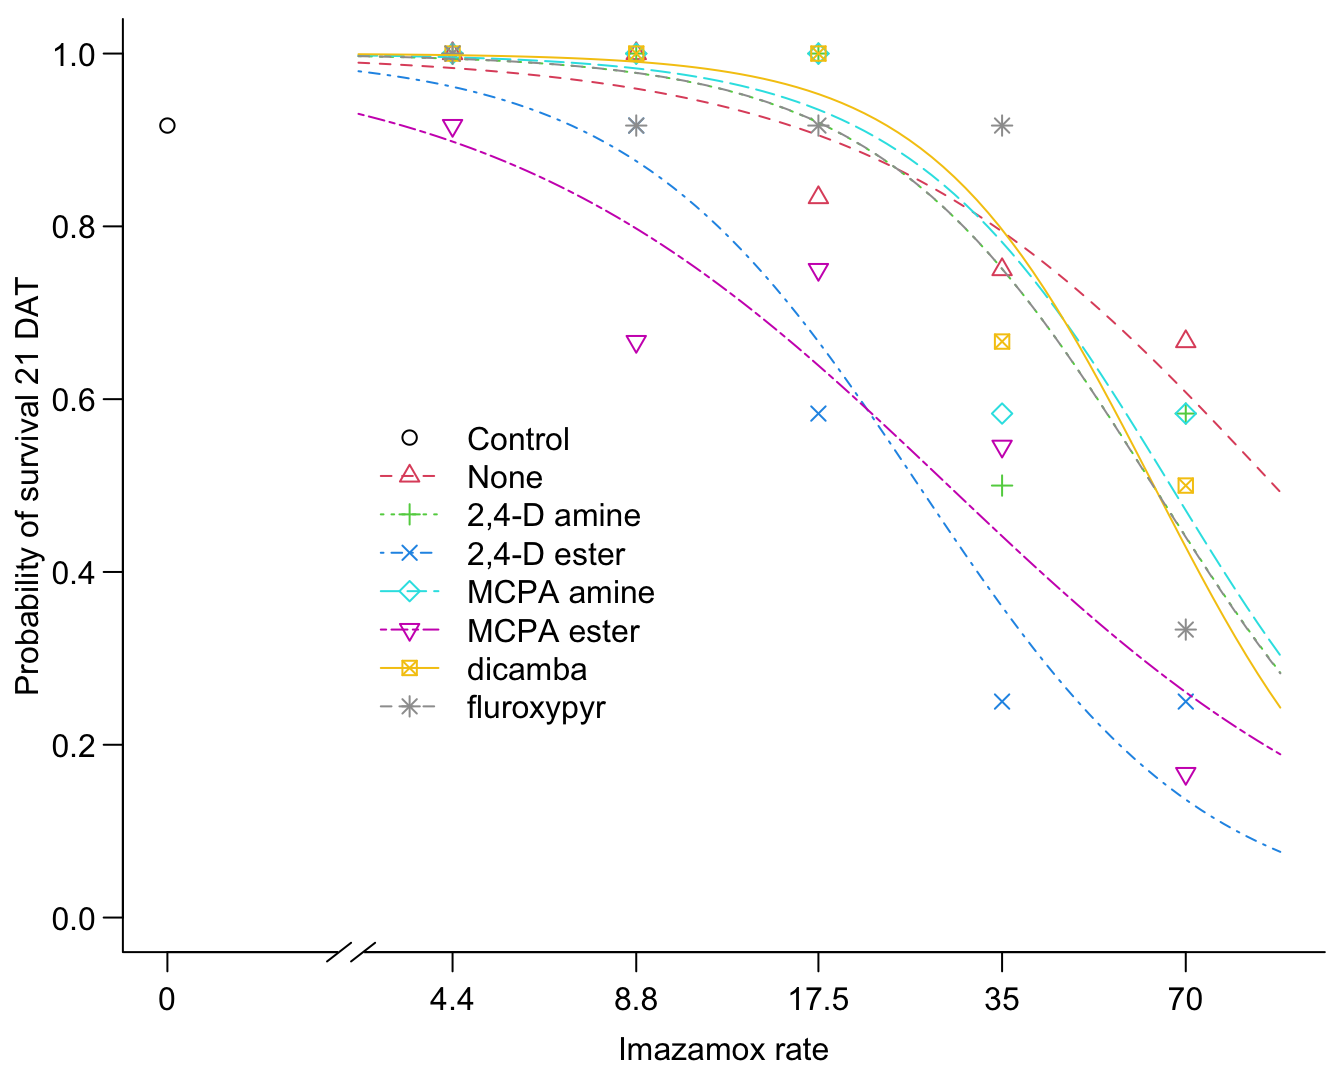
\includegraphics{Rstats4ag_files/figure-latex/figlogisticrye-1.pdf}
\caption{\label{fig:figlogisticrye}\emph{The effect of imazamox rate with and without auxin-mimic herbicides on rye survival.}}
\end{figure}

\begin{center}\rule{0.5\linewidth}{0.5pt}\end{center}

\hypertarget{dose-response-curves}{%
\chapter{Dose-Response curves}\label{dose-response-curves}}

We are surrounded by synthetic and natural substances that have both positive and negative effects upon humans, other animals, and the environment. It is difficult to estimate effects of a substance without testing it on living organisms. Chemical and physical properties of a substance can tell us about the molecules themselves, but living organisms may react in unpredictable ways. Therefore, we use biological assay to estimate effects. It means the design of bioassay experiments and the modelling of the response as a function of the dose is crucial for the classification of chemical compounds. In order to understand the principles of bioassay it is imperative to link results with the real world exposure to chemicals. In this chapter, chemicals used to illustrate bioassay are pesticides, but the principles are the same whatever the chemical.

\href{\%22http://www.jstor.org/stable/1403201?origin=crossref\&seq=1\#page_scan_tab_contents\%22}{Finney 1976} wrote: ``As a branch of applied statistics, biological assay appears to have a somewhat specialized appeal. Although a few statisticians have worked in it intensively, to the majority it appears as a topic that can be neglected, either because of its difficulties or because it is trivial\ldots{}\ldots{}. I am convinced that many features of bioassay are out-standingly good for concentrating the mind on important parts of biometric practice and statistical inference.''

In biology there are four general curves that describe many biological phenomena. Two of them, the rectangular hyperbola (of which Michaelis-Menten is a notable example) and sigmoid curves have either one or two asymptotes; that is, they have upper and/or lower limits as the independent variable approaches very small or very large values.

In most text books, non-linear regression is not very well explained although it is easy for practitioners to implement. The difference between linear and non-linear regression can often be boiled down to the very fact: linear regression can be solved analytically by least square analysis, whereas the nonlinear regression cannot.

Before fitting a nonlinear regression model, one has to do some guesstimates about the initial regression parameters before fitting. In some cases a nonlinear relationship can be converted to a linear one. The most common one is the exponential curve (Figure 1 that turns into a linear relationship when taking the logarithm of the \texttt{y}. For the rectangular hyperbola it is usually with no lower limit and then it can also be linearize by manipulating as in ezymeology and biochemistry.The rectangular hyperbola is in other disciplines called the Michaelis Menten model.

This chapter will be devoted to the use of the add-on package `drc? and will illustrate some of the facilities built in the package so far.



\begin{figure}
\centering
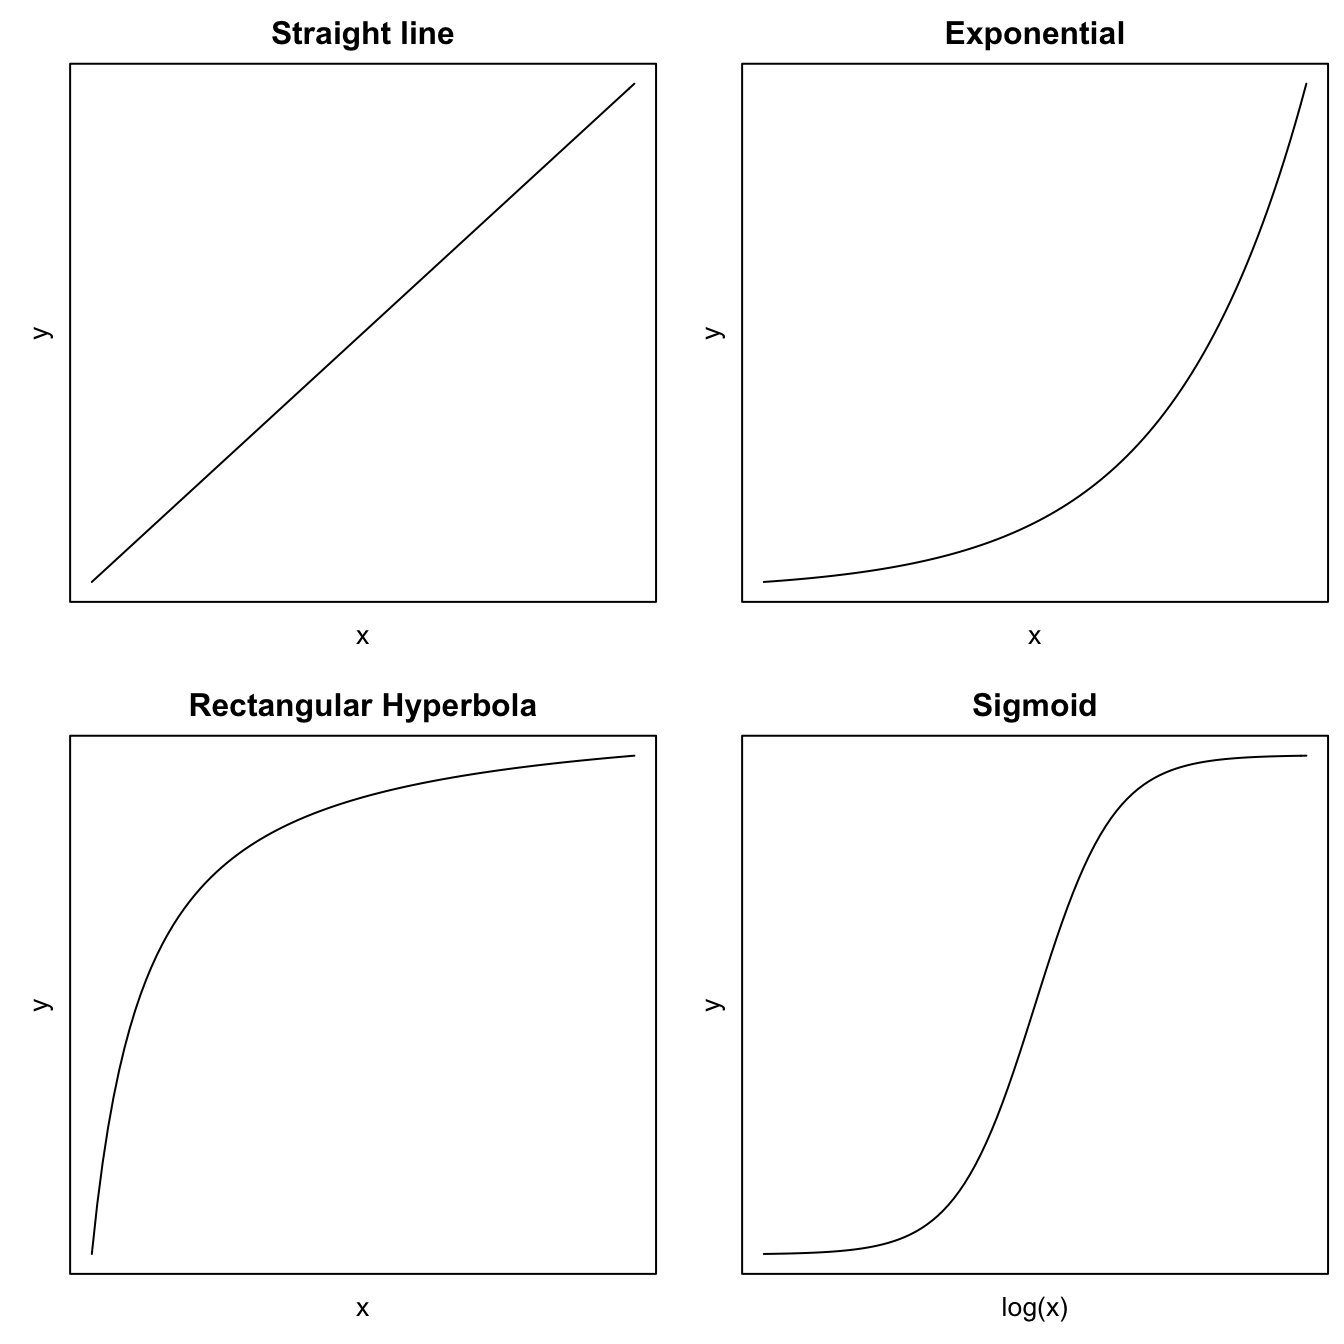
\includegraphics{Rstats4ag_files/figure-latex/figcommonmodel4panel-1.pdf}
\caption{\label{fig:figcommonmodel4panel}\emph{Common regressions models in the biological sciences.}}
\end{figure}

For the sigmoid curves, which can take several forms, we have to use nonlinear regression. One of the most common curves is the symmetric log-logistic model:

\[y = c+\frac{d-c}{1+exp(b(log(x)-log(ED50)))} .\]

\texttt{y} is the response, \texttt{c} denotes the lower limit of the response when the dose \texttt{x} approaches infinity; \texttt{d} is the upper limit when the dose \texttt{x} approaches 0. \texttt{b} denotes the slope around the point of inflection, which is the \(ED_{50}\), i.e.~the dose required to reduce the response half-way between the upper and lower limit.

Guessing the parameters of a sigmoid curve can, for the less experienced person, be tiresome and frustrating. This has now been overcome by the development of a package named \texttt{drc}, which was developed at the University of Copenhagen. The purpose of the \texttt{drc} package was to ease the analysis of dose-response curves from greenhouse and field experiments in Weed and Pesticide Science courses and to assess the selectivity of herbicides and efficacy of pesticides. Similar dose-response curves are commonly used in ecotoxicology and general toxicology, and the \texttt{drc} package is used in various other disciplines.

Gradually, \texttt{drc} has been extended with numerous nonlinear curves commonly used in the life sciences and elsewhere. The engine of \texttt{drc} is the \texttt{drm(y\textasciitilde{}x,\ fct=...)} function with self-starter that automatically calculates initial parameters. The \texttt{fct=}argument identifies the particular dose-response curve to be used. An overview of the various functions available can be accessed, after loading the \texttt{drc} package, by typing \texttt{?getMeanFunctions()}.

\hypertarget{one-dose-response-curve}{%
\section{One Dose-Response Curve}\label{one-dose-response-curve}}

Let us look at how to fit a dose-response curve using a training data set in the \texttt{drc} package.

\begin{Shaded}
\begin{Highlighting}[]
\KeywordTok{library}\NormalTok{(drc)}
\end{Highlighting}
\end{Shaded}

Before curve fitting, it is important to get an idea of how the data look. Below we create a plot with the x variable both on original scale and on log scale.



\begin{Shaded}
\begin{Highlighting}[]
\KeywordTok{head}\NormalTok{(ryegrass,}\DecValTok{3}\NormalTok{) }
\end{Highlighting}
\end{Shaded}

\begin{verbatim}
##      rootl conc
## 1 7.580000    0
## 2 8.000000    0
## 3 8.328571    0
\end{verbatim}

\begin{Shaded}
\begin{Highlighting}[]
\NormalTok{op <-}\StringTok{ }\KeywordTok{par}\NormalTok{(}\DataTypeTok{mfrow =} \KeywordTok{c}\NormalTok{(}\DecValTok{1}\NormalTok{, }\DecValTok{2}\NormalTok{), }\DataTypeTok{mar=}\KeywordTok{c}\NormalTok{(}\FloatTok{3.2}\NormalTok{,}\FloatTok{3.2}\NormalTok{,}\DecValTok{2}\NormalTok{,.}\DecValTok{5}\NormalTok{), }\DataTypeTok{mgp=}\KeywordTok{c}\NormalTok{(}\DecValTok{2}\NormalTok{,.}\DecValTok{7}\NormalTok{,}\DecValTok{0}\NormalTok{)) }\CommentTok{#make two plots in two columns }
\KeywordTok{plot}\NormalTok{(rootl }\OperatorTok{~}\StringTok{ }\NormalTok{conc, }\DataTypeTok{data =}\NormalTok{ ryegrass, }\DataTypeTok{main=}\StringTok{"Original Dose Scale"}\NormalTok{)}
\KeywordTok{plot}\NormalTok{(rootl }\OperatorTok{~}\StringTok{ }\KeywordTok{log}\NormalTok{(conc}\FloatTok{+.1}\NormalTok{), }\DataTypeTok{data =}\NormalTok{ ryegrass, }\DataTypeTok{main=}\StringTok{"Logarithmic Dose Scale"}\NormalTok{)}
\end{Highlighting}
\end{Shaded}

\begin{figure}
\centering
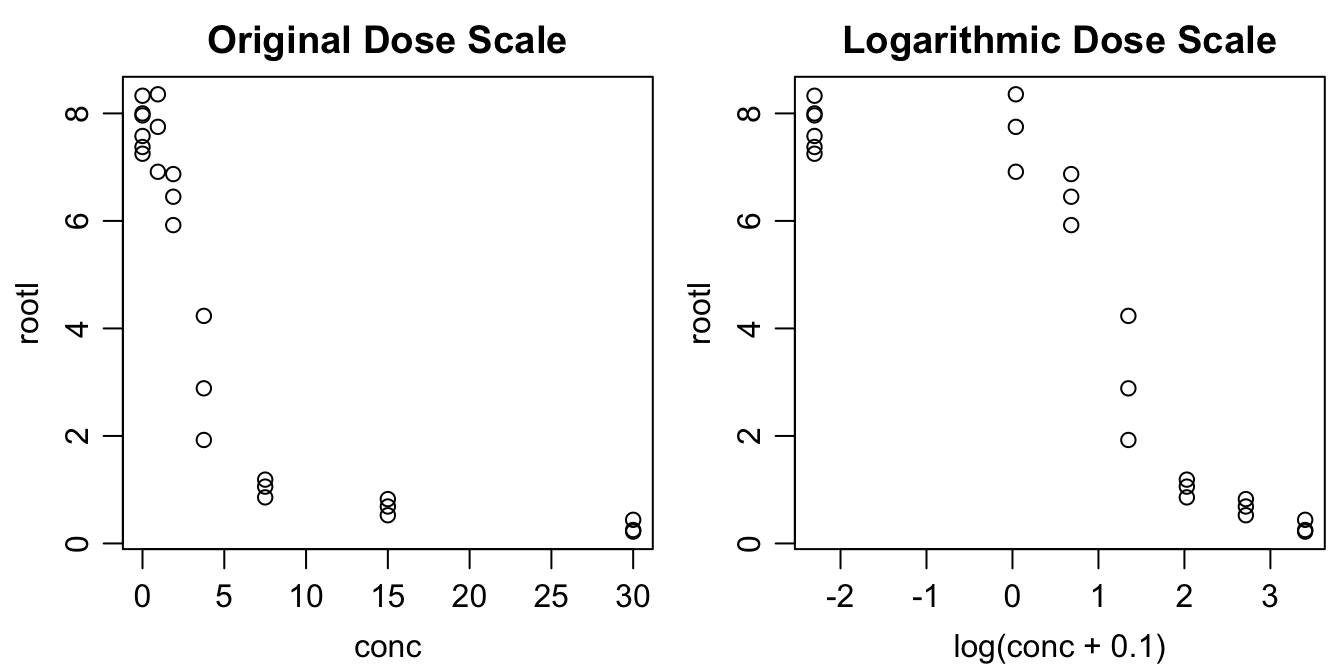
\includegraphics{Rstats4ag_files/figure-latex/figdrrootlpanel-1.pdf}
\caption{\label{fig:figdrrootlpanel}\emph{There are two ways of plotting dose-response data, the default in the \texttt{drc} package is to use a logarithmic scale for x. Note with the logarithmic dose scale the untreated control, 0, is not defined. That is why we add 0.1 to the concentration before taking the logarithm.}}
\end{figure}

Below we fit a four-parameter log-logistic model with user-defined parameter names. The default names of the parameters (\emph{b}, \emph{c}, \emph{d}, and \emph{e}) included in the \texttt{drm()} function might not make sense to many weed scientists, but the \texttt{names=c()} argument can be used to facilitate sharing output with less seasoned \texttt{drc} users. The four parameter log-logistic curve has an upper limit, \texttt{d}, lower limit, \texttt{c}, the \(ED_{50}\) is denoted \texttt{e}, and finally the slope, \texttt{b}, around the \(ED_{50}\).

\begin{Shaded}
\begin{Highlighting}[]
\NormalTok{ryegrass.m1 <-}\StringTok{ }\KeywordTok{drm}\NormalTok{(rootl }\OperatorTok{~}\StringTok{ }\NormalTok{conc, }\DataTypeTok{data =}\NormalTok{ ryegrass, }
                   \DataTypeTok{fct =} \KeywordTok{LL.4}\NormalTok{(}\DataTypeTok{names =} \KeywordTok{c}\NormalTok{(}\StringTok{"Slope"}\NormalTok{, }\StringTok{"Lower Limit"}\NormalTok{, }\StringTok{"Upper Limit"}\NormalTok{, }\StringTok{"ED50"}\NormalTok{)))}
\KeywordTok{summary}\NormalTok{(ryegrass.m1)}
\end{Highlighting}
\end{Shaded}

\begin{verbatim}
## 
## Model fitted: Log-logistic (ED50 as parameter) (4 parms)
## 
## Parameter estimates:
## 
##                         Estimate Std. Error t-value   p-value    
## Slope:(Intercept)        2.98222    0.46506  6.4125 2.960e-06 ***
## Lower Limit:(Intercept)  0.48141    0.21219  2.2688   0.03451 *  
## Upper Limit:(Intercept)  7.79296    0.18857 41.3272 < 2.2e-16 ***
## ED50:(Intercept)         3.05795    0.18573 16.4644 4.268e-13 ***
## ---
## Signif. codes:  0 '***' 0.001 '**' 0.01 '*' 0.05 '.' 0.1 ' ' 1
## 
## Residual standard error:
## 
##  0.5196256 (20 degrees of freedom)
\end{verbatim}

The summary of the curve fitting shows the estimates of each of the four parameters and their standard errors. The p-values tell us if the parameters are different from zero. In this instance all four parameters are significantly different from zero and as seen on the graph the log-logistic curve seems to fit well to data.



\begin{Shaded}
\begin{Highlighting}[]
\NormalTok{op <-}\StringTok{ }\KeywordTok{par}\NormalTok{(}\DataTypeTok{mfrow =} \KeywordTok{c}\NormalTok{(}\DecValTok{1}\NormalTok{, }\DecValTok{2}\NormalTok{), }\DataTypeTok{mar=}\KeywordTok{c}\NormalTok{(}\FloatTok{3.2}\NormalTok{,}\FloatTok{3.2}\NormalTok{,.}\DecValTok{5}\NormalTok{,.}\DecValTok{5}\NormalTok{), }\DataTypeTok{mgp=}\KeywordTok{c}\NormalTok{(}\DecValTok{2}\NormalTok{,.}\DecValTok{7}\NormalTok{,}\DecValTok{0}\NormalTok{))}
\KeywordTok{plot}\NormalTok{(ryegrass.m1, }\DataTypeTok{broken=}\OtherTok{TRUE}\NormalTok{, }\DataTypeTok{bty=}\StringTok{"l"}\NormalTok{,}
     \DataTypeTok{xlab=}\StringTok{"Concentration of Ferulic Acid"}\NormalTok{, }\DataTypeTok{ylab=}\StringTok{"Length of Roots"}\NormalTok{)}
\KeywordTok{plot}\NormalTok{(ryegrass.m1, }\DataTypeTok{broken=}\OtherTok{TRUE}\NormalTok{, }\DataTypeTok{bty=}\StringTok{"l"}\NormalTok{,}
     \DataTypeTok{xlab=}\StringTok{"Concentration of Ferulic Acid"}\NormalTok{, }\DataTypeTok{ylab=}\StringTok{"Length of Roots"}\NormalTok{,}\DataTypeTok{type=}\StringTok{"all"}\NormalTok{)}
\end{Highlighting}
\end{Shaded}

\begin{figure}
\centering
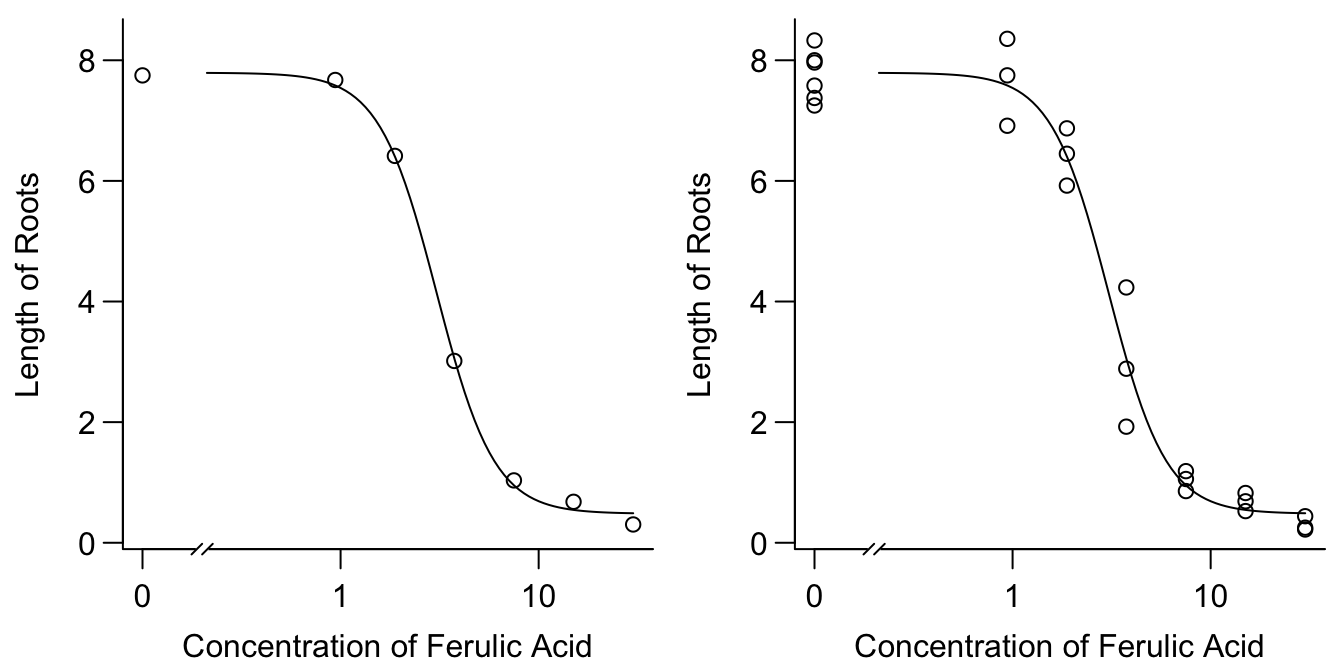
\includegraphics{Rstats4ag_files/figure-latex/figrootpanelmodel-1.pdf}
\caption{\label{fig:figrootpanelmodel}\emph{Plot of regression and averages of observations within each concentration (left), and all observation (right).}}
\end{figure}

The slope of the dose-response curve at \(ED_{50}\) has the opposite sign as compared to the sign of the parameter \texttt{b}. This is the consequence of the parameterization used in \texttt{drc} for the log-logistic model, a choice that is in part rooted in what was commonly used in the past. The actual slope of the tangent of the curve at \(ED_{50}\) is determined :

\[\frac{-b}{(d-c)/(4*e)}\]

So apart from the sign there is a scaling factor that converts the parameter \texttt{b} into the slope, Therefore, the use of the word ``relative''. Note that the scaling factor may be viewed as a kind of normalization factor involving the range of the response. As a consequence estimated \texttt{b} values often lie in the range 0.5 to 20 in absolute value, regardless of the assay or experiment generating the data.

Note at the end of the ryegrass help file \texttt{?ryegrass} you can see examples, which give you some ideas of what can be done. The ryegrass help provides examples of various sigmoid curves to show the differences among them (see later). Note that we use the argument \texttt{broken=TRUE} to break the x-axis, because on a logarithmic scale, which is the default in \texttt{drc}, there is no such thing as a zero dose.

There are various ways to check if a regression model gives a satisfactory picture of the variation in data. Before doing further analysis, the best way to judge it is to look at the graph to see if there are some serious discrepancies between the regression and mean values. Being satisfied with the results of the fit, one way of checking is to test for lack of fit against the most general model, an ANOVA. It is done automatically in drc with the function \texttt{modelFit()}.

\begin{Shaded}
\begin{Highlighting}[]
\CommentTok{#Test for lack of fit}
\KeywordTok{modelFit}\NormalTok{(ryegrass.m1)}
\end{Highlighting}
\end{Shaded}

\begin{verbatim}
## Lack-of-fit test
## 
##           ModelDf    RSS Df F value p value
## ANOVA          17 5.1799                   
## DRC model      20 5.4002  3  0.2411  0.8665
\end{verbatim}

Obviously, the test for lack of fit is non-significant and therefore we can tentatively entertain the idea that the regression analysis was just as good to describe the variation in data as was an ANOVA. The test for lack of fit is not enough to ensure the fit is reasonable, because of few degrees of freedom, in this instance only 3 degrees of freedom. Another issue is that the more doses we use the less likely it is that the test for lack of fit would become non-significant; the mere fact being that the log-logistic curve, like any other sigmoid curve, is just an approximation of the real relationship.

The distribution of the residuals and the hopefully normal distribution of residuals are informative to make sure that the prerequisites for doing a regression in the first place are not violated. The assumptions we must consider include:

\begin{enumerate}
\def\labelenumi{\arabic{enumi}.}
\tightlist
\item
  Correct regression model
\item
  Variance Homogeneity
\item
  Normally distributed measurement errors
\item
  Mutually independent measurement error \(\varepsilon\)
\end{enumerate}

Number 1 can always be discussed and we will not go too much into detail. This is generally determined by researchers familiar with the phenomena being described. Number 2 is important if you want to infer on the variability of parameters. Normally, the parameter estimates do not change much whether there are homogeneous variance or not; it is the standard errors that change and that is why we want to come so close to homogeneity of variance as possible. This is important when comparing curves, or evaluating the certainty we have about various parameters (like the effective dose or upper limit). Number 3 can be graphically shown and is only in some instances critical. Number 4 is important because we assume the observations for doses are independent of each other, a question that also can be debated. When we do dose-response experiments we often use the same stock solution. It means that any systematic error can be carried all the way though the dilution process and be part of the dose. Below we illustrate items 2 and item 3.



\begin{Shaded}
\begin{Highlighting}[]
\CommentTok{#Graphical analysis of residuals}
\NormalTok{op <-}\StringTok{ }\KeywordTok{par}\NormalTok{(}\DataTypeTok{mfrow =} \KeywordTok{c}\NormalTok{(}\DecValTok{1}\NormalTok{, }\DecValTok{2}\NormalTok{), }\DataTypeTok{mar=}\KeywordTok{c}\NormalTok{(}\FloatTok{3.2}\NormalTok{,}\FloatTok{3.2}\NormalTok{,}\DecValTok{2}\NormalTok{,.}\DecValTok{5}\NormalTok{), }\DataTypeTok{mgp=}\KeywordTok{c}\NormalTok{(}\DecValTok{2}\NormalTok{,.}\DecValTok{7}\NormalTok{,}\DecValTok{0}\NormalTok{)) }\CommentTok{#put two graphs together}
    \KeywordTok{plot}\NormalTok{(}\KeywordTok{residuals}\NormalTok{(ryegrass.m1) }\OperatorTok{~}\StringTok{ }\KeywordTok{fitted}\NormalTok{(ryegrass.m1), }\DataTypeTok{main=}\StringTok{"Residuals vs Fitted"}\NormalTok{)}
\KeywordTok{abline}\NormalTok{(}\DataTypeTok{h=}\DecValTok{0}\NormalTok{)}
\KeywordTok{qqnorm}\NormalTok{(}\KeywordTok{residuals}\NormalTok{(ryegrass.m1))}
 \KeywordTok{qqline}\NormalTok{(}\KeywordTok{residuals}\NormalTok{(ryegrass.m1))}
\end{Highlighting}
\end{Shaded}

\begin{figure}
\centering
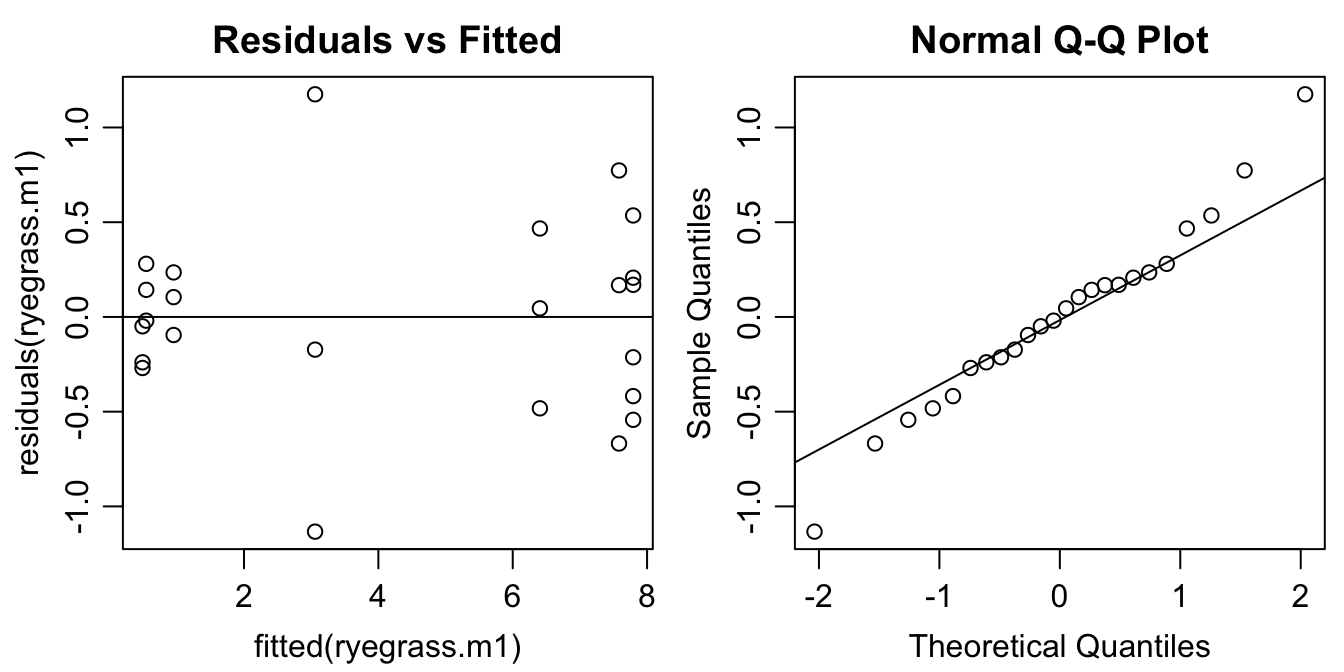
\includegraphics{Rstats4ag_files/figure-latex/rootdiag-1.pdf}
\caption{\label{fig:rootdiag}\emph{Model esiduals diagnostic plots: Left: distribution of residuals against the fitted value (variance homogeneity); Right: normal q-q plot illustrating whether the residuals are normally distributed (normally distributed measurement errors).}}
\end{figure}

The residual plot indicates that the model was able to catch the variation in data. The distribution of residuals should look like a shotgun shot on a wall. Apparently, there are some systematic violations in the residual plot, At small fitted values the residuals are close to zero than at high fitted values the variation is much more pronounced. This is called a funnel type pattern. We also see it in the graphs with the fit and all the observations (Figure \ref{fig:rootdiag}). The normal Q-Q plot looks all right, no serious deviation from the assumption of normal distribution of residuals. Later we will look at this problem, which is a statistical problem not a biological one.

\hypertarget{note-on-use-of-r2}{%
\section{\texorpdfstring{Note on use of \(R^2\)}{Note on use of R\^{}2}}\label{note-on-use-of-r2}}

One of the most popular ways of assessing goodness of fit in regression, be it linear or nonlinear, is to use \(R^2\). The higher the better, but the \(R^2\) does \emph{not} tell you how well the curve fits to the data. In fact, if there are large differences between the maximum and the minimum observation, the \(R^2\) will be larger than if the differences are small. It is also important to note that the most common interpretation of \(R^2\) for linear regression does not hold true for nonlinear regression; in the nonlinear case, the \(R^2\) value is \emph{not} the amount of variability in Y explained by X. At its core, the \href{http://www.jstor.org/stable/2684259}{\(R^2\) is a comparison of 2 models}; in linear regression the two models being compared are the regression model and a null model indicating no relationship between X and Y. For nonlinear regression, the choice of a `null' model is not as simple, and therefore the \(R^2\) type measure will be different depending on the chosen reduced model. The appropriate `null' model may differ (and perhaps \emph{should} differ) depending on the nonlinear model being used. Therefore, the \(R^2\) is not part of the output from \texttt{drc}. To give an example we fit a linear model to the ryegrass data.



\begin{Shaded}
\begin{Highlighting}[]
\NormalTok{op <-}\StringTok{ }\KeywordTok{par}\NormalTok{(}\DataTypeTok{mfrow =} \KeywordTok{c}\NormalTok{(}\DecValTok{1}\NormalTok{, }\DecValTok{2}\NormalTok{), }\DataTypeTok{mar=}\KeywordTok{c}\NormalTok{(}\FloatTok{3.2}\NormalTok{,}\FloatTok{3.2}\NormalTok{,}\DecValTok{0}\NormalTok{,.}\DecValTok{5}\NormalTok{), }\DataTypeTok{mgp=}\KeywordTok{c}\NormalTok{(}\DecValTok{2}\NormalTok{,.}\DecValTok{7}\NormalTok{,}\DecValTok{0}\NormalTok{)) }\CommentTok{#put two graphs together}
\KeywordTok{plot}\NormalTok{(rootl }\OperatorTok{~}\StringTok{ }\NormalTok{conc, }\DataTypeTok{data =}\NormalTok{ ryegrass, }\DataTypeTok{bty=}\StringTok{"l"}\NormalTok{)}
\NormalTok{linear.m1 <-}\StringTok{ }\KeywordTok{lm}\NormalTok{(rootl }\OperatorTok{~}\StringTok{ }\NormalTok{conc, }\DataTypeTok{data =}\NormalTok{ ryegrass)}
\KeywordTok{summary}\NormalTok{(linear.m1)}
\end{Highlighting}
\end{Shaded}

\begin{verbatim}
## 
## Call:
## lm(formula = rootl ~ conc, data = ryegrass)
## 
## Residuals:
##     Min      1Q  Median      3Q     Max 
## -3.4399 -1.7055  0.9623  1.7532  2.3575 
## 
## Coefficients:
##             Estimate Std. Error t value Pr(>|t|)    
## (Intercept)  6.24176    0.52973  11.783 5.64e-11 ***
## conc        -0.25929    0.04326  -5.994 4.94e-06 ***
## ---
## Signif. codes:  0 '***' 0.001 '**' 0.01 '*' 0.05 '.' 0.1 ' ' 1
## 
## Residual standard error: 2.07 on 22 degrees of freedom
## Multiple R-squared:  0.6202, Adjusted R-squared:  0.603 
## F-statistic: 35.93 on 1 and 22 DF,  p-value: 4.939e-06
\end{verbatim}

\begin{Shaded}
\begin{Highlighting}[]
\KeywordTok{abline}\NormalTok{(linear.m1)}
\KeywordTok{plot}\NormalTok{(linear.m1, }\DataTypeTok{which=}\DecValTok{1}\NormalTok{, }\DataTypeTok{bty=}\StringTok{"l"}\NormalTok{)}
\end{Highlighting}
\end{Shaded}

\begin{figure}
\centering
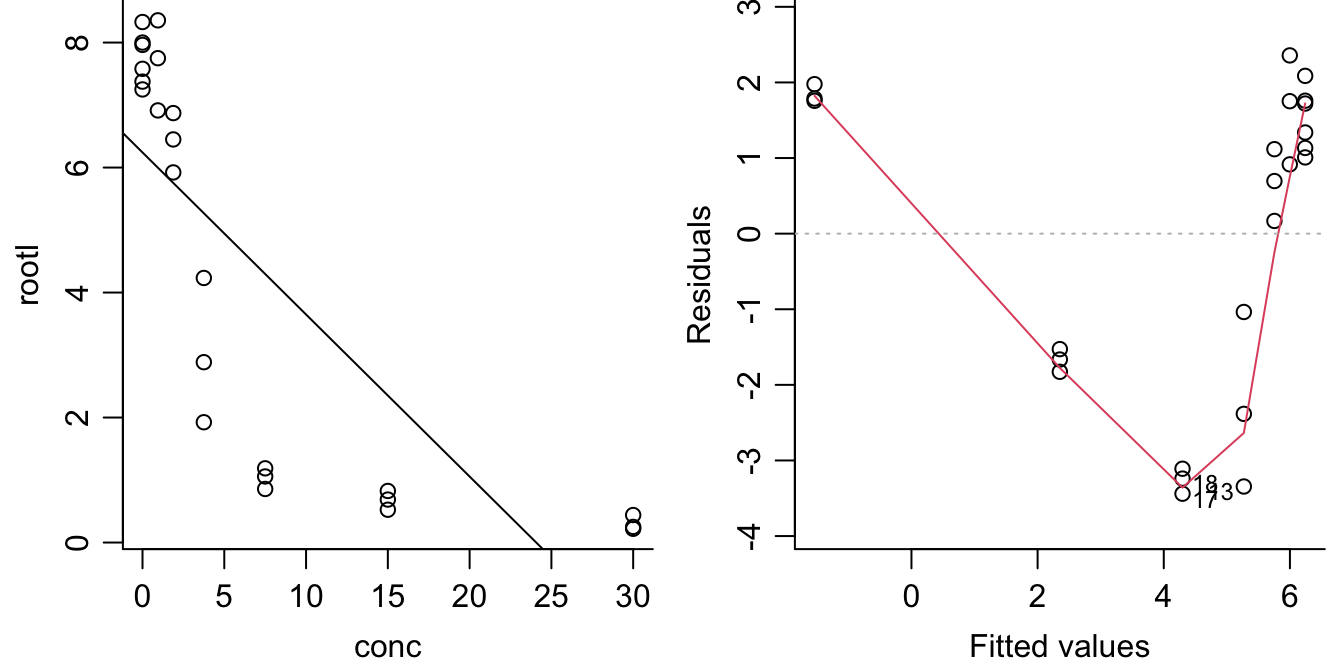
\includegraphics{Rstats4ag_files/figure-latex/figr2ex-1.pdf}
\caption{\label{fig:figr2ex}\emph{Linear regression y=-.25x+6.24 with highly significant parameters (left) and residual plot (right). The \(R^2\) is not negligable (\(R^2\) = 0.6), but the model is obviously not correct.}}
\end{figure}

The regression parameters are highly significantly different from zero so it looks good as does \(R^2\) of 0.62 . This is not a small value, but obviously the goodness of fit is not good, let alone the systematic distribution of residuals. When trying to determine whether the nonlinear model is better or worse than the linear model, Akaike Information Criterion (AIC) can be used. Smaller values of AIC indicate better fit to the data.

\begin{Shaded}
\begin{Highlighting}[]
\KeywordTok{AIC}\NormalTok{(ryegrass.m1, linear.m1)}
\end{Highlighting}
\end{Shaded}

\begin{verbatim}
##             df       AIC
## ryegrass.m1  5  42.31029
## linear.m1    3 106.95109
\end{verbatim}

The AIC value for the nonlinear model \texttt{ryegrass.m1} is much lower than the linear fit \texttt{linear.m1} that definitely violated item 1. This confirms that the nonlinear model is a better fit to the data compared with the linear model.

\hypertarget{which-dose-response-model}{%
\section{Which Dose-Response Model?}\label{which-dose-response-model}}

There exists numerous sigmoid curves of which the log-logistic is the most common one. It is symmetric and the \(ED_{50}\) is a parameter of the model. Several other models exist, particularly, the non symmetric ones where \(ED_{50}\) is not a ``natural'' parameter. For example the Weibull-1 model.

\[y = c+(d-c)exp(-exp(b(log(x)-log(e)))) .\]

The parameter \texttt{b} is the steepness of the curve and the
parameter \texttt{e} is the dose where the inflection point of the dose-
response curve is located, which is \emph{not} the \(ED_{50}\).The Weibull-1 descends slowly from the upper limit \texttt{d} and approach the lower limit \texttt{c} rapidly.

Another model, Weibull-2 is somewhat different from Weibull-1, because it has a different asymmetry, with a rapid descent from the upper limit \texttt{d} and a slow approach toward the lower limit (Figure \ref{fig:fignlinmodelcomp}).

\[y = c+(d-c)(1-exp(-exp(b(log(x)-log(e))))) .\]

\href{http://onlinelibrary.wiley.com/doi/10.1002/etc.7/abstract}{Ritz 2009} has in detailed described those asymmetric dose-response curves and also illustrated it as shown in Figure \ref{fig:fignlinmodelcomp}.



\begin{Shaded}
\begin{Highlighting}[]
\KeywordTok{library}\NormalTok{(drc)}
\CommentTok{## Comparing log-logistic and Weibull models}
\CommentTok{## (Figure 2 in Ritz (2009))}
\NormalTok{ryegrass.m0 <-}\StringTok{ }\KeywordTok{drm}\NormalTok{(rootl }\OperatorTok{~}\StringTok{ }\NormalTok{conc, }\DataTypeTok{data =}\NormalTok{ ryegrass, }\DataTypeTok{fct =} \KeywordTok{LL.4}\NormalTok{())}
\NormalTok{ryegrass.m1 <-}\StringTok{ }\KeywordTok{drm}\NormalTok{(rootl }\OperatorTok{~}\StringTok{ }\NormalTok{conc, }\DataTypeTok{data =}\NormalTok{ ryegrass, }\DataTypeTok{fct =} \KeywordTok{W1.4}\NormalTok{())}
\NormalTok{ryegrass.m2 <-}\StringTok{ }\KeywordTok{drm}\NormalTok{(rootl }\OperatorTok{~}\StringTok{ }\NormalTok{conc, }\DataTypeTok{data =}\NormalTok{ ryegrass, }\DataTypeTok{fct =} \KeywordTok{W2.4}\NormalTok{())}

\KeywordTok{par}\NormalTok{(}\DataTypeTok{mfrow=}\KeywordTok{c}\NormalTok{(}\DecValTok{1}\NormalTok{,}\DecValTok{1}\NormalTok{), }\DataTypeTok{mar=}\KeywordTok{c}\NormalTok{(}\FloatTok{3.2}\NormalTok{,}\FloatTok{3.2}\NormalTok{,.}\DecValTok{5}\NormalTok{,.}\DecValTok{5}\NormalTok{), }\DataTypeTok{mgp=}\KeywordTok{c}\NormalTok{(}\DecValTok{2}\NormalTok{,.}\DecValTok{7}\NormalTok{,}\DecValTok{0}\NormalTok{))}
\KeywordTok{plot}\NormalTok{(ryegrass.m0, }\DataTypeTok{broken=}\OtherTok{TRUE}\NormalTok{, }\DataTypeTok{xlab=}\StringTok{"Dose (mM)"}\NormalTok{, }\DataTypeTok{ylab=}\StringTok{"Root length (cm)"}\NormalTok{, }\DataTypeTok{lwd=}\DecValTok{2}\NormalTok{, }
     \DataTypeTok{cex=}\FloatTok{1.2}\NormalTok{, }\DataTypeTok{cex.axis=}\FloatTok{1.2}\NormalTok{, }\DataTypeTok{cex.lab=}\FloatTok{1.2}\NormalTok{, }\DataTypeTok{bty=}\StringTok{"l"}\NormalTok{)}
\KeywordTok{plot}\NormalTok{(ryegrass.m1, }\DataTypeTok{add=}\OtherTok{TRUE}\NormalTok{, }\DataTypeTok{broken=}\OtherTok{TRUE}\NormalTok{, }\DataTypeTok{lty=}\DecValTok{2}\NormalTok{, }\DataTypeTok{lwd=}\DecValTok{2}\NormalTok{)}
\KeywordTok{plot}\NormalTok{(ryegrass.m2, }\DataTypeTok{add=}\OtherTok{TRUE}\NormalTok{, }\DataTypeTok{broken=}\OtherTok{TRUE}\NormalTok{, }\DataTypeTok{lty=}\DecValTok{3}\NormalTok{, }\DataTypeTok{lwd=}\DecValTok{2}\NormalTok{)}

\KeywordTok{arrows}\NormalTok{(}\DecValTok{3}\NormalTok{, }\FloatTok{7.5}\NormalTok{, }\FloatTok{1.4}\NormalTok{, }\FloatTok{7.5}\NormalTok{, }\FloatTok{0.15}\NormalTok{, }\DataTypeTok{lwd=}\DecValTok{2}\NormalTok{)}
\KeywordTok{text}\NormalTok{(}\DecValTok{3}\NormalTok{,}\FloatTok{7.5}\NormalTok{, }\StringTok{"Weibull-2"}\NormalTok{, }\DataTypeTok{pos=}\DecValTok{4}\NormalTok{, }\DataTypeTok{cex=}\FloatTok{1.2}\NormalTok{)}

\KeywordTok{arrows}\NormalTok{(}\FloatTok{2.5}\NormalTok{, }\FloatTok{0.9}\NormalTok{, }\FloatTok{5.7}\NormalTok{, }\FloatTok{0.9}\NormalTok{, }\FloatTok{0.15}\NormalTok{, }\DataTypeTok{lwd=}\DecValTok{2}\NormalTok{)}
\KeywordTok{text}\NormalTok{(}\DecValTok{3}\NormalTok{,}\FloatTok{0.9}\NormalTok{, }\StringTok{"Weibull-1"}\NormalTok{, }\DataTypeTok{pos=}\DecValTok{2}\NormalTok{, }\DataTypeTok{cex=}\FloatTok{1.2}\NormalTok{)}
\end{Highlighting}
\end{Shaded}

\begin{figure}
\centering
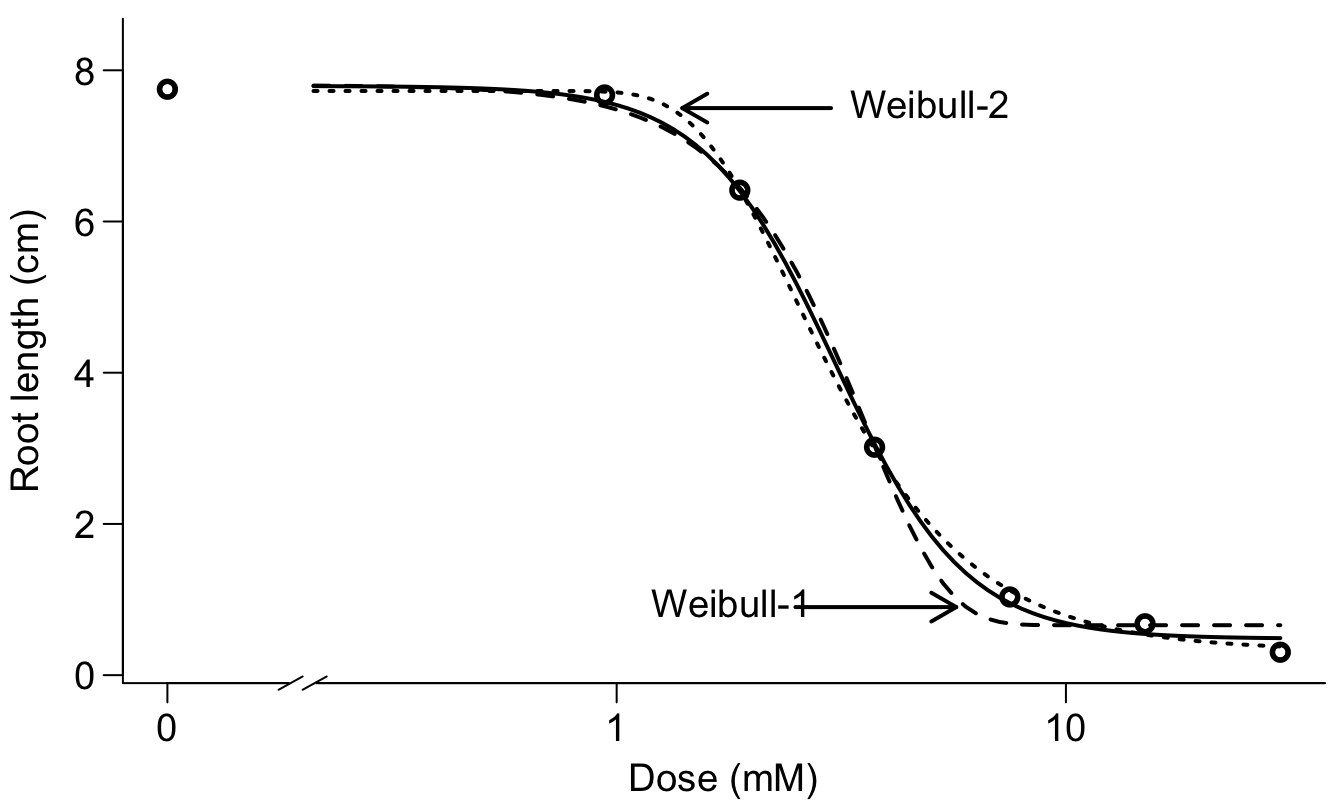
\includegraphics{Rstats4ag_files/figure-latex/fignlinmodelcomp-1.pdf}
\caption{\label{fig:fignlinmodelcomp}\emph{Comparison among the two asymmetric Weibull models and the log-logistic model. The differences in this instance are at either the upper limit or the lower limit of the curves.}}
\end{figure}

The \(ED_{50}\) for the Weibull-1 and Weibull-2 model has to be derived from the fit by using the function\texttt{ED()}.

\begin{Shaded}
\begin{Highlighting}[]
 \KeywordTok{ED}\NormalTok{(ryegrass.m1,}\DecValTok{50}\NormalTok{,}\DataTypeTok{interval=}\StringTok{"delta"}\NormalTok{)}
\end{Highlighting}
\end{Shaded}

\begin{verbatim}
## 
## Estimated effective doses
## 
##        Estimate Std. Error   Lower   Upper
## e:1:50  3.08896    0.17331 2.72744 3.45048
\end{verbatim}

A relevant questions would be how do the \(ED_{x}\) change when fitting the different sigmoid curves?

To illustrate this we use the ggplot2 package and a function to combine graphs. First we have to calculate the \(ED_{x}\) and combine the results in a data.frame as done below.

\begin{Shaded}
\begin{Highlighting}[]
\NormalTok{edLL<-}\KeywordTok{data.frame}\NormalTok{(}\KeywordTok{ED}\NormalTok{(ryegrass.m0,}\KeywordTok{c}\NormalTok{(}\DecValTok{10}\NormalTok{,}\DecValTok{50}\NormalTok{,}\DecValTok{90}\NormalTok{),}\DataTypeTok{interval=}\StringTok{"delta"}\NormalTok{, }
                    \DataTypeTok{display=}\OtherTok{FALSE}\NormalTok{),}\DataTypeTok{ll=}\StringTok{"Log-logistic"}\NormalTok{)            }
\NormalTok{edW1<-}\KeywordTok{data.frame}\NormalTok{(}\KeywordTok{ED}\NormalTok{(ryegrass.m1,}\KeywordTok{c}\NormalTok{(}\DecValTok{10}\NormalTok{,}\DecValTok{50}\NormalTok{,}\DecValTok{90}\NormalTok{),}\DataTypeTok{interval=}\StringTok{"delta"}\NormalTok{, }
                    \DataTypeTok{display=}\OtherTok{FALSE}\NormalTok{),}\DataTypeTok{ll=}\StringTok{"Weibull 1"}\NormalTok{)}
\NormalTok{edW2<-}\KeywordTok{data.frame}\NormalTok{(}\KeywordTok{ED}\NormalTok{(ryegrass.m2,}\KeywordTok{c}\NormalTok{(}\DecValTok{10}\NormalTok{,}\DecValTok{50}\NormalTok{,}\DecValTok{90}\NormalTok{),}\DataTypeTok{interval=}\StringTok{"delta"}\NormalTok{, }
                    \DataTypeTok{display=}\OtherTok{FALSE}\NormalTok{),}\DataTypeTok{ll=}\StringTok{"Weibull 2"}\NormalTok{)}
\NormalTok{CombED<-}\KeywordTok{rbind}\NormalTok{(edLL,edW1,edW2)}
\end{Highlighting}
\end{Shaded}

Then we can use \texttt{plot\_grid()} from the \texttt{cowplot} package, which is a function that combines various independent ggplots into one plot.



\begin{Shaded}
\begin{Highlighting}[]
\KeywordTok{library}\NormalTok{(ggplot2)}
\KeywordTok{library}\NormalTok{(cowplot)}

\NormalTok{p1 <-}\StringTok{ }\KeywordTok{ggplot}\NormalTok{(}\DataTypeTok{data=}\NormalTok{CombED[}\KeywordTok{c}\NormalTok{(}\DecValTok{1}\NormalTok{,}\DecValTok{4}\NormalTok{,}\DecValTok{7}\NormalTok{),], }\KeywordTok{aes}\NormalTok{(}\DataTypeTok{x=}\NormalTok{ll, }\DataTypeTok{y=}\NormalTok{Estimate))}\OperatorTok{+}
\StringTok{ }\KeywordTok{geom_bar}\NormalTok{(}\DataTypeTok{stat=}\StringTok{"identity"}\NormalTok{, }\DataTypeTok{fill=}\StringTok{"lightgreen"}\NormalTok{, }\DataTypeTok{colour=}\StringTok{"black"}\NormalTok{)}\OperatorTok{+}
\StringTok{  }\KeywordTok{geom_errorbar}\NormalTok{(}\KeywordTok{aes}\NormalTok{(}\DataTypeTok{ymin=}\NormalTok{Lower, }\DataTypeTok{ymax=}\NormalTok{Upper), }\DataTypeTok{width=}\FloatTok{0.1}\NormalTok{) }\OperatorTok{+}
\StringTok{  }\KeywordTok{ylab}\NormalTok{(}\StringTok{"ED10"}\NormalTok{)}\OperatorTok{+}
\StringTok{  }\KeywordTok{xlab}\NormalTok{(}\StringTok{""}\NormalTok{)}
\NormalTok{p2 <-}\StringTok{ }\KeywordTok{ggplot}\NormalTok{(}\DataTypeTok{data=}\NormalTok{CombED[}\KeywordTok{c}\NormalTok{(}\DecValTok{2}\NormalTok{,}\DecValTok{5}\NormalTok{,}\DecValTok{8}\NormalTok{),], }\KeywordTok{aes}\NormalTok{(}\DataTypeTok{x=}\NormalTok{ll, }\DataTypeTok{y=}\NormalTok{Estimate))}\OperatorTok{+}
\StringTok{  }\KeywordTok{geom_bar}\NormalTok{(}\DataTypeTok{stat=}\StringTok{"identity"}\NormalTok{, }\DataTypeTok{fill=}\StringTok{"lightgreen"}\NormalTok{, }\DataTypeTok{colour=}\StringTok{"black"}\NormalTok{)}\OperatorTok{+}
\StringTok{  }\KeywordTok{geom_errorbar}\NormalTok{(}\KeywordTok{aes}\NormalTok{(}\DataTypeTok{ymin=}\NormalTok{Lower, }\DataTypeTok{ymax=}\NormalTok{Upper), }\DataTypeTok{width=}\FloatTok{0.1}\NormalTok{) }\OperatorTok{+}
\StringTok{  }\KeywordTok{ylab}\NormalTok{(}\StringTok{"ED50"}\NormalTok{)}\OperatorTok{+}
\StringTok{  }\KeywordTok{xlab}\NormalTok{(}\StringTok{""}\NormalTok{)}

\NormalTok{p3 <-}\StringTok{ }\KeywordTok{ggplot}\NormalTok{(}\DataTypeTok{data=}\NormalTok{CombED[}\KeywordTok{c}\NormalTok{(}\DecValTok{3}\NormalTok{,}\DecValTok{6}\NormalTok{,}\DecValTok{9}\NormalTok{),], }\KeywordTok{aes}\NormalTok{(}\DataTypeTok{x=}\NormalTok{ll, }\DataTypeTok{y=}\NormalTok{Estimate))}\OperatorTok{+}
\KeywordTok{geom_bar}\NormalTok{(}\DataTypeTok{stat=}\StringTok{"identity"}\NormalTok{, }\DataTypeTok{fill=}\StringTok{"lightgreen"}\NormalTok{, }\DataTypeTok{colour=}\StringTok{"black"}\NormalTok{)}\OperatorTok{+}
\StringTok{  }\KeywordTok{geom_errorbar}\NormalTok{(}\KeywordTok{aes}\NormalTok{(}\DataTypeTok{ymin=}\NormalTok{Lower, }\DataTypeTok{ymax=}\NormalTok{Upper), }\DataTypeTok{width=}\FloatTok{0.1}\NormalTok{) }\OperatorTok{+}
\StringTok{  }\KeywordTok{ylab}\NormalTok{(}\StringTok{"ED90"}\NormalTok{)}\OperatorTok{+}
\StringTok{  }\KeywordTok{xlab}\NormalTok{(}\StringTok{"Sigmoid four parameter models"}\NormalTok{)}

\KeywordTok{plot_grid}\NormalTok{(p1,p2,p3, }\DataTypeTok{ncol=}\DecValTok{1}\NormalTok{)}
\end{Highlighting}
\end{Shaded}

\begin{figure}
\centering
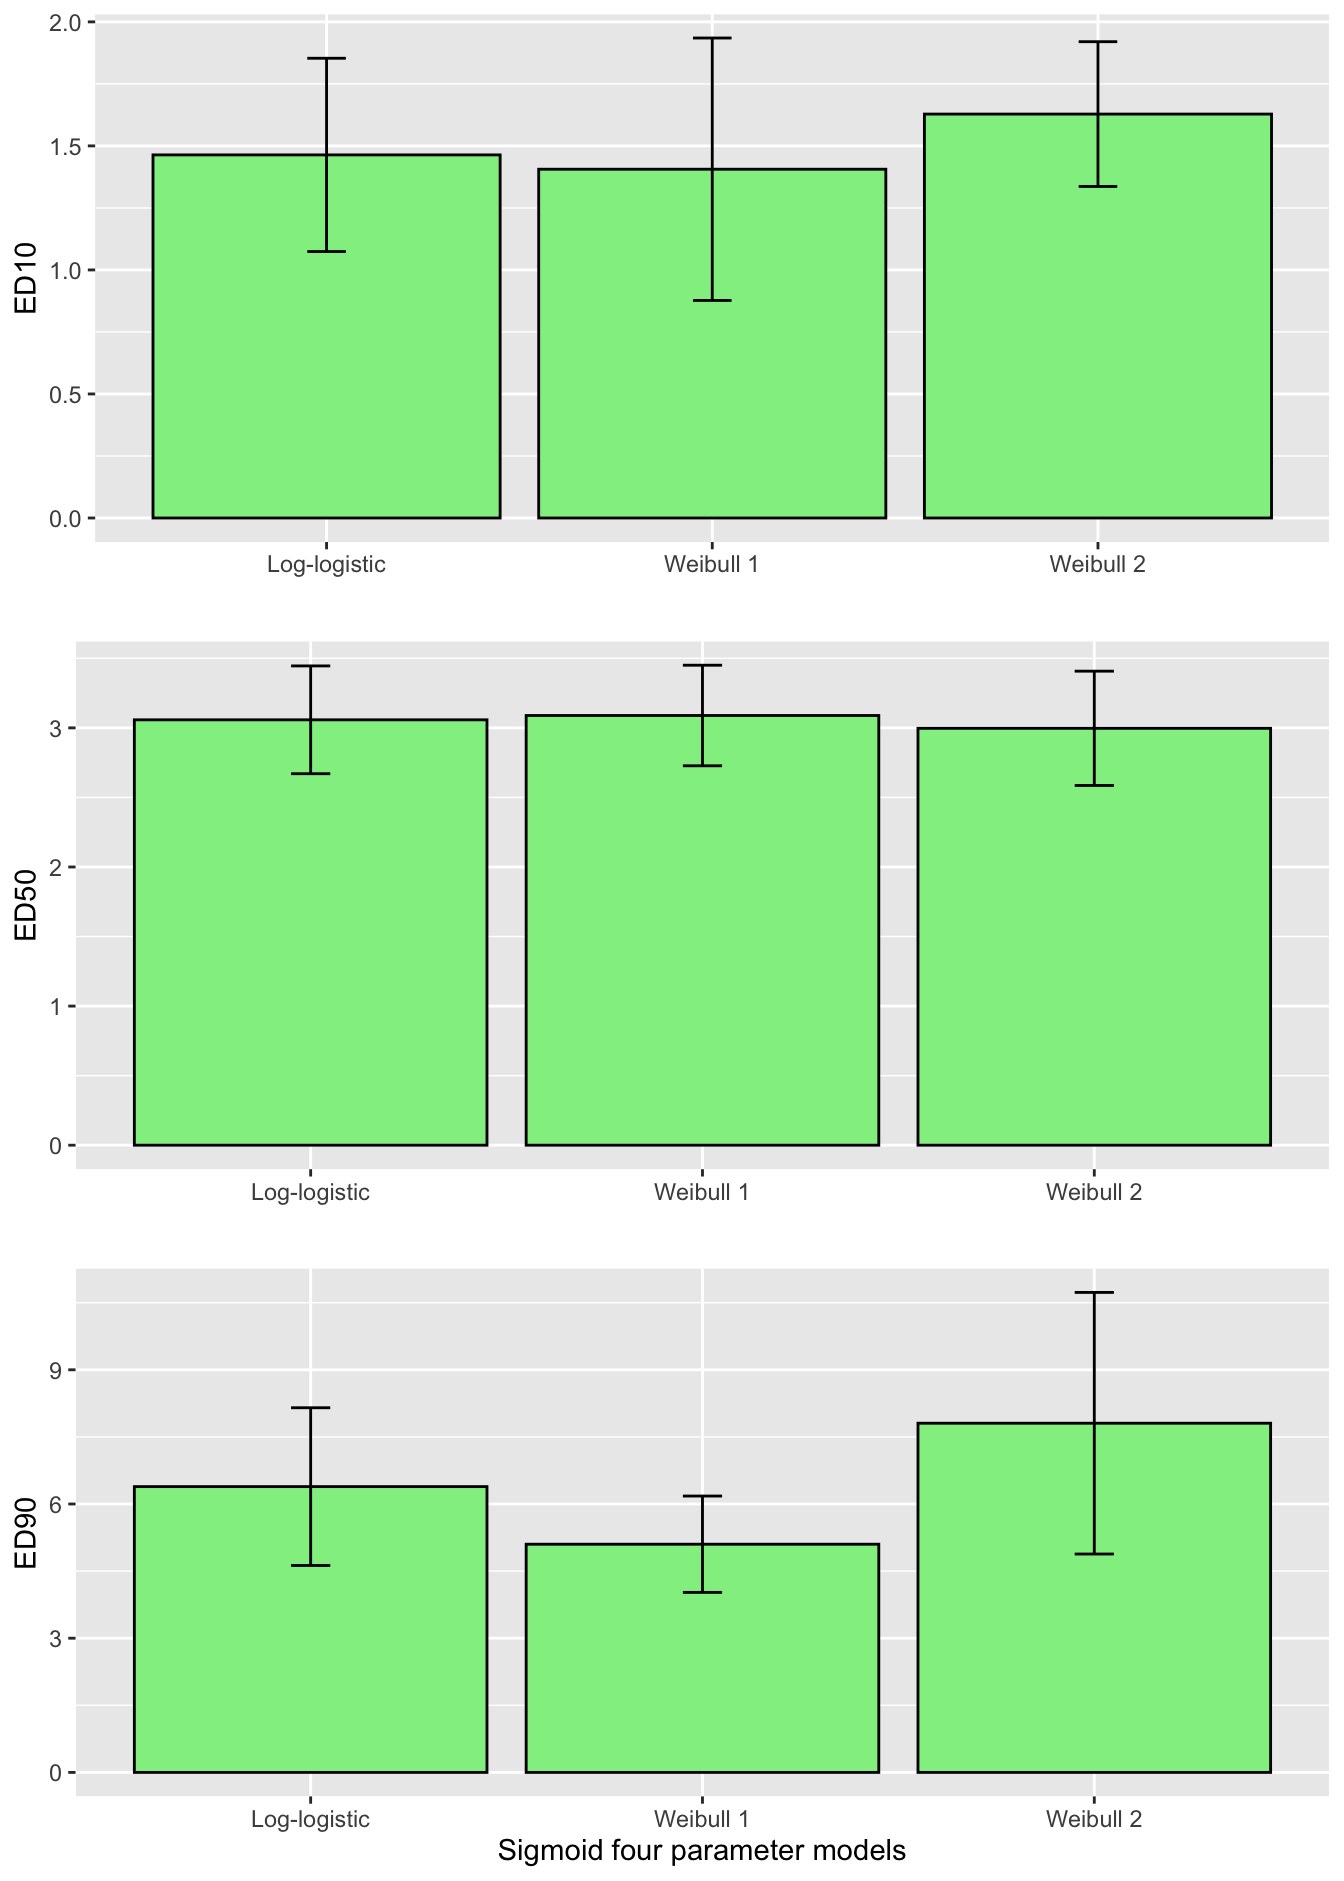
\includegraphics{Rstats4ag_files/figure-latex/figEDcomp-1.pdf}
\caption{\label{fig:figEDcomp}\emph{Comparison of \(ED_{10}\), \(ED_{50}\) and \(ED_{90}\) for various sigmoid dose-response curves with associated 95\% confidence intervals.}}
\end{figure}

Obviously, the ED-levels in Figure \ref{fig:figEDcomp} in this instance did not change much among the three sigmoid curves. Sometimes they do and residual plots show that one of the asymmetrical curves is more appropriate than the common log-logistic, although it can not be substantiated by an ordinary test for lack of fit.\texttt{drc}also has a function where you can test the differences between the \(ED_{x}\) as shown below

\begin{Shaded}
\begin{Highlighting}[]
\KeywordTok{comped}\NormalTok{(CombED[}\KeywordTok{c}\NormalTok{(}\DecValTok{1}\NormalTok{,}\DecValTok{4}\NormalTok{),}\DecValTok{1}\NormalTok{],CombED[}\KeywordTok{c}\NormalTok{(}\DecValTok{1}\NormalTok{,}\DecValTok{4}\NormalTok{),}\DecValTok{2}\NormalTok{],}\DataTypeTok{log=}\NormalTok{F,}\DataTypeTok{operator =} \StringTok{"-"}\NormalTok{)}
\end{Highlighting}
\end{Shaded}

\begin{verbatim}
## 
## Estimated difference of effective doses
## 
##       Estimate Std. Error     Lower Upper
## [1,]  0.057726   0.314927 -0.559519 0.675
\end{verbatim}

\begin{Shaded}
\begin{Highlighting}[]
\KeywordTok{comped}\NormalTok{(CombED[}\KeywordTok{c}\NormalTok{(}\DecValTok{1}\NormalTok{,}\DecValTok{7}\NormalTok{),}\DecValTok{1}\NormalTok{],CombED[}\KeywordTok{c}\NormalTok{(}\DecValTok{1}\NormalTok{,}\DecValTok{7}\NormalTok{),}\DecValTok{2}\NormalTok{],}\DataTypeTok{log=}\NormalTok{F,}\DataTypeTok{operator =} \StringTok{"-"}\NormalTok{)}
\end{Highlighting}
\end{Shaded}

\begin{verbatim}
## 
## Estimated difference of effective doses
## 
##      Estimate Std. Error    Lower  Upper
## [1,] -0.16457    0.23335 -0.62193 0.2928
\end{verbatim}

\begin{Shaded}
\begin{Highlighting}[]
\KeywordTok{comped}\NormalTok{(CombED[}\KeywordTok{c}\NormalTok{(}\DecValTok{3}\NormalTok{,}\DecValTok{6}\NormalTok{),}\DecValTok{1}\NormalTok{],CombED[}\KeywordTok{c}\NormalTok{(}\DecValTok{3}\NormalTok{,}\DecValTok{6}\NormalTok{),}\DecValTok{2}\NormalTok{],}\DataTypeTok{log=}\NormalTok{F,}\DataTypeTok{operator =} \StringTok{"-"}\NormalTok{)}
\end{Highlighting}
\end{Shaded}

\begin{verbatim}
## 
## Estimated difference of effective doses
## 
##      Estimate Std. Error    Lower  Upper
## [1,]  1.28762    0.99032 -0.65337 3.2286
\end{verbatim}

\begin{Shaded}
\begin{Highlighting}[]
\KeywordTok{comped}\NormalTok{(CombED[}\KeywordTok{c}\NormalTok{(}\DecValTok{6}\NormalTok{,}\DecValTok{9}\NormalTok{),}\DecValTok{1}\NormalTok{],CombED[}\KeywordTok{c}\NormalTok{(}\DecValTok{6}\NormalTok{,}\DecValTok{9}\NormalTok{),}\DecValTok{2}\NormalTok{],}\DataTypeTok{log=}\NormalTok{F,}\DataTypeTok{operator =} \StringTok{"-"}\NormalTok{)}
\end{Highlighting}
\end{Shaded}

\begin{verbatim}
## 
## Estimated difference of effective doses
## 
##      Estimate Std. Error   Lower  Upper
## [1,]  -2.7048     1.4939 -5.6327 0.2231
\end{verbatim}

\begin{Shaded}
\begin{Highlighting}[]
\KeywordTok{comped}\NormalTok{(CombED[}\KeywordTok{c}\NormalTok{(}\DecValTok{3}\NormalTok{,}\DecValTok{9}\NormalTok{),}\DecValTok{1}\NormalTok{],CombED[}\KeywordTok{c}\NormalTok{(}\DecValTok{3}\NormalTok{,}\DecValTok{9}\NormalTok{),}\DecValTok{2}\NormalTok{],}\DataTypeTok{log=}\NormalTok{F,}\DataTypeTok{operator =} \StringTok{"-"}\NormalTok{)}
\end{Highlighting}
\end{Shaded}

\begin{verbatim}
## 
## Estimated difference of effective doses
## 
##      Estimate Std. Error   Lower Upper
## [1,]  -1.4172     1.6368 -4.6253 1.791
\end{verbatim}

\begin{Shaded}
\begin{Highlighting}[]
\KeywordTok{comped}\NormalTok{(CombED[}\KeywordTok{c}\NormalTok{(}\DecValTok{6}\NormalTok{,}\DecValTok{9}\NormalTok{),}\DecValTok{1}\NormalTok{],CombED[}\KeywordTok{c}\NormalTok{(}\DecValTok{6}\NormalTok{,}\DecValTok{9}\NormalTok{),}\DecValTok{2}\NormalTok{],}\DataTypeTok{log=}\NormalTok{F,}\DataTypeTok{operator =} \StringTok{"-"}\NormalTok{)}
\end{Highlighting}
\end{Shaded}

\begin{verbatim}
## 
## Estimated difference of effective doses
## 
##      Estimate Std. Error   Lower  Upper
## [1,]  -2.7048     1.4939 -5.6327 0.2231
\end{verbatim}

None of the differences are significantly different form zero, lower limits are negative in all instance and upper limits of the differences are positive.

\hypertarget{more-dose-response-curves}{%
\section{More Dose-Response Curves}\label{more-dose-response-curves}}

When it comes to assessment of herbicide selectivity, one dose-response curve does not tell you anything. Selectivity of a herbicide is always dose-dependent and a bioassay with a pre-fixed harvest day only gives a snapshot of the effect of a herbicide. When comparing dose-response curves of say two herbicides on the same plant species or one herbicide on two plant species, it is imperative that the curves you compare were run at the same point in time or at least close to and at the same stage of plant development. The training data set \texttt{S.alba} in the \texttt{drc} package consists of two dose-response curves, one for bentazon and one for glyphosate.

\begin{Shaded}
\begin{Highlighting}[]
\KeywordTok{head}\NormalTok{(S.alba,}\DataTypeTok{n=}\DecValTok{2}\NormalTok{)}
\end{Highlighting}
\end{Shaded}

\begin{verbatim}
##   Dose  Herbicide DryMatter
## 1    0 Glyphosate       4.7
## 2    0 Glyphosate       4.6
\end{verbatim}

\begin{Shaded}
\begin{Highlighting}[]
\KeywordTok{tail}\NormalTok{(S.alba,}\DataTypeTok{n=}\DecValTok{2}\NormalTok{)}
\end{Highlighting}
\end{Shaded}

\begin{verbatim}
##    Dose Herbicide DryMatter
## 67  640 Bentazone       0.6
## 68  640 Bentazone       0.8
\end{verbatim}

\begin{Shaded}
\begin{Highlighting}[]
\CommentTok{## Fitting a log-logistic model with}
\NormalTok{S.alba.m1 <-}\StringTok{ }\KeywordTok{drm}\NormalTok{(DryMatter }\OperatorTok{~}\StringTok{ }\NormalTok{Dose, Herbicide, }\DataTypeTok{data=}\NormalTok{S.alba, }\DataTypeTok{fct =} \KeywordTok{LL.4}\NormalTok{())}
\end{Highlighting}
\end{Shaded}

Note that the the variable, Herbicide, identifies the herbicides, Therefore, the third argument in the \texttt{drm()} is the classification variable \texttt{Herbicide}.

\begin{Shaded}
\begin{Highlighting}[]
\KeywordTok{modelFit}\NormalTok{(S.alba.m1)}
\end{Highlighting}
\end{Shaded}

\begin{verbatim}
## Lack-of-fit test
## 
##           ModelDf    RSS Df F value p value
## ANOVA          53 8.0800                   
## DRC model      60 8.3479  7  0.2511  0.9696
\end{verbatim}

\begin{Shaded}
\begin{Highlighting}[]
\KeywordTok{summary}\NormalTok{(S.alba.m1)}
\end{Highlighting}
\end{Shaded}

\begin{verbatim}
## 
## Model fitted: Log-logistic (ED50 as parameter) (4 parms)
## 
## Parameter estimates:
## 
##               Estimate Std. Error t-value   p-value    
## b:Glyphosate  2.715409   0.748279  3.6289 0.0005897 ***
## b:Bentazone   5.134810   1.130949  4.5403 2.760e-05 ***
## c:Glyphosate  0.891238   0.194703  4.5774 2.421e-05 ***
## c:Bentazone   0.681845   0.095111  7.1689 1.288e-09 ***
## d:Glyphosate  3.875759   0.107463 36.0661 < 2.2e-16 ***
## d:Bentazone   3.805791   0.110341 34.4911 < 2.2e-16 ***
## e:Glyphosate 62.087606   6.611444  9.3909 2.184e-13 ***
## e:Bentazone  29.268444   2.237090 13.0833 < 2.2e-16 ***
## ---
## Signif. codes:  0 '***' 0.001 '**' 0.01 '*' 0.05 '.' 0.1 ' ' 1
## 
## Residual standard error:
## 
##  0.3730047 (60 degrees of freedom)
\end{verbatim}

The test for lack of fit shows non-significance, and furthermore, the summary shows that the upper limits \texttt{d}s are very close to each other and the same applies to the lower limit \texttt{c}s. Consequently, we could entertain the idea that they are similar for both curves. We use the argument in the \texttt{drm()} function \texttt{pmodels=data.frame(..)}to make the upper limit and the lower limit similar for both curves. The argument follows the alphabetical order of the names of the parameters, \texttt{b,c,d,e}. Below, we will allow the \texttt{b} parameter to vary freely between the two herbicides, whereas \texttt{c} and \texttt{d} will be held the same for both herbicides (they have the same identification \texttt{1,1}). Finally the \texttt{e} parameters can vary freely.



\begin{Shaded}
\begin{Highlighting}[]
\CommentTok{##  common lower and upper limits}
\NormalTok{S.alba.m2 <-}\StringTok{ }\KeywordTok{drm}\NormalTok{(DryMatter }\OperatorTok{~}\StringTok{ }\NormalTok{Dose, Herbicide, }\DataTypeTok{data=}\NormalTok{S.alba, }\DataTypeTok{fct =} \KeywordTok{LL.4}\NormalTok{(),}
                 \DataTypeTok{pmodels=}\KeywordTok{data.frame}\NormalTok{(Herbicide, }\DecValTok{1}\NormalTok{, }\DecValTok{1}\NormalTok{, Herbicide)) }
\KeywordTok{summary}\NormalTok{(S.alba.m2)}
\end{Highlighting}
\end{Shaded}

\begin{verbatim}
## 
## Model fitted: Log-logistic (ED50 as parameter) (4 parms)
## 
## Parameter estimates:
## 
##                Estimate Std. Error t-value   p-value    
## b:Bentazone    5.046141   1.040135  4.8514 8.616e-06 ***
## b:Glyphosate   2.390218   0.495959  4.8194 9.684e-06 ***
## c:(Intercept)  0.716559   0.089245  8.0291 3.523e-11 ***
## d:(Intercept)  3.854861   0.076255 50.5519 < 2.2e-16 ***
## e:Bentazone   28.632355   2.038098 14.0486 < 2.2e-16 ***
## e:Glyphosate  66.890545   5.968819 11.2067 < 2.2e-16 ***
## ---
## Signif. codes:  0 '***' 0.001 '**' 0.01 '*' 0.05 '.' 0.1 ' ' 1
## 
## Residual standard error:
## 
##  0.3705151 (62 degrees of freedom)
\end{verbatim}

\begin{Shaded}
\begin{Highlighting}[]
\KeywordTok{par}\NormalTok{(}\DataTypeTok{mfrow=}\KeywordTok{c}\NormalTok{(}\DecValTok{1}\NormalTok{,}\DecValTok{1}\NormalTok{), }\DataTypeTok{mar=}\KeywordTok{c}\NormalTok{(}\FloatTok{3.2}\NormalTok{,}\FloatTok{3.2}\NormalTok{,.}\DecValTok{5}\NormalTok{,.}\DecValTok{5}\NormalTok{), }\DataTypeTok{mgp=}\KeywordTok{c}\NormalTok{(}\DecValTok{2}\NormalTok{,.}\DecValTok{7}\NormalTok{,}\DecValTok{0}\NormalTok{))}
\KeywordTok{plot}\NormalTok{(S.alba.m1, }\DataTypeTok{broken=}\OtherTok{TRUE}\NormalTok{, }\DataTypeTok{bty=}\StringTok{"l"}\NormalTok{)}
\KeywordTok{plot}\NormalTok{(S.alba.m2, }\DataTypeTok{col=}\StringTok{"red"}\NormalTok{, }\DataTypeTok{broken=}\OtherTok{TRUE}\NormalTok{, }\DataTypeTok{add=}\OtherTok{TRUE}\NormalTok{, }\DataTypeTok{legend=}\OtherTok{FALSE}\NormalTok{)}
\end{Highlighting}
\end{Shaded}

\begin{figure}
\centering
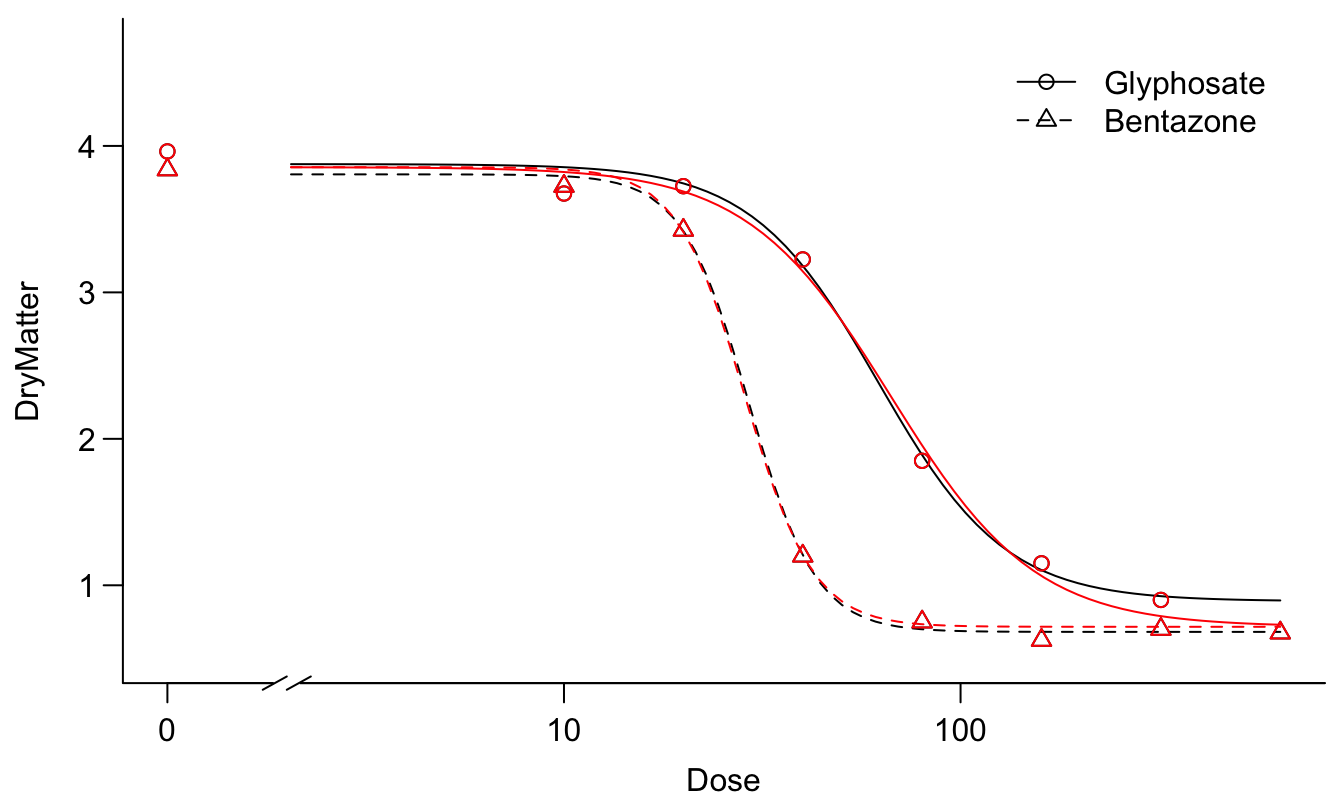
\includegraphics{Rstats4ag_files/figure-latex/figglybentnlin-1.pdf}
\caption{\label{fig:figglybentnlin}\emph{The two fits, one without assuming common upper and lower limits for the two curves (black) and one where the curves have the same upper and lower limits (red).}}
\end{figure}

\begin{Shaded}
\begin{Highlighting}[]
\KeywordTok{anova}\NormalTok{(S.alba.m1, S.alba.m2) }\CommentTok{# Test for lack of fit not signifiancant}
\end{Highlighting}
\end{Shaded}

\begin{verbatim}
## 
## 1st model
##  fct:     LL.4()
##  pmodels: Herbicide, 1, 1, Herbicide
## 2nd model
##  fct:     LL.4()
##  pmodels: Herbicide (for all parameters)
\end{verbatim}

\begin{verbatim}
## ANOVA table
## 
##           ModelDf    RSS Df F value p value
## 2nd model      62 8.5114                   
## 1st model      60 8.3479  2  0.5876  0.5588
\end{verbatim}

A test for lack of fit was non-significant and, therefore, we presume that the curves have similar upper an lower limits. Now we have the ideal framework for comparing the relative potency between the two herbicides with similar upper and lower limit, we have the same reference for both curves.

Comparing the fit without freely estimated upper and lower limit and with common upper and lower limit did not change the \(ED_{50}\) much but did reduce the standard errors somewhat.

The next step could be to assume that the two curves also have the same slope, i.e.~the two curves are similar and only differ in their relative displacement along the x-axis.

\begin{Shaded}
\begin{Highlighting}[]
\CommentTok{##  common lower and upper limits and slope}
\NormalTok{S.alba.m3 <-}\StringTok{ }\KeywordTok{drm}\NormalTok{(DryMatter}\OperatorTok{~}\NormalTok{Dose, Herbicide, }\DataTypeTok{data=}\NormalTok{S.alba, }\DataTypeTok{fct =} \KeywordTok{LL.4}\NormalTok{(),}
                 \DataTypeTok{pmodels=}\KeywordTok{data.frame}\NormalTok{(}\DecValTok{1}\NormalTok{, }\DecValTok{1}\NormalTok{, }\DecValTok{1}\NormalTok{, Herbicide)) }
\KeywordTok{anova}\NormalTok{(S.alba.m2, S.alba.m3)}
\end{Highlighting}
\end{Shaded}

\begin{verbatim}
## 
## 1st model
##  fct:     LL.4()
##  pmodels: 1, 1, 1, Herbicide
## 2nd model
##  fct:     LL.4()
##  pmodels: Herbicide, 1, 1, Herbicide
\end{verbatim}

\begin{verbatim}
## ANOVA table
## 
##           ModelDf    RSS Df F value p value
## 2nd model      63 9.4946                   
## 1st model      62 8.5114  1  7.1614  0.0095
\end{verbatim}

Although the `parallel' curves in Figure \ref{fig:figglybentslope} seem reasonable, the test for lack of fit now is significant, so the assumption of similar curves except for the \(ED_{50}\) is not supported. We should prefer, instead, the model with independent slopes (Figure \ref{fig:figglybentnlin}).



\begin{Shaded}
\begin{Highlighting}[]
\KeywordTok{par}\NormalTok{(}\DataTypeTok{mfrow=}\KeywordTok{c}\NormalTok{(}\DecValTok{1}\NormalTok{,}\DecValTok{1}\NormalTok{), }\DataTypeTok{mar=}\KeywordTok{c}\NormalTok{(}\FloatTok{3.2}\NormalTok{,}\FloatTok{3.2}\NormalTok{,.}\DecValTok{5}\NormalTok{,.}\DecValTok{5}\NormalTok{), }\DataTypeTok{mgp=}\KeywordTok{c}\NormalTok{(}\DecValTok{2}\NormalTok{,.}\DecValTok{7}\NormalTok{,}\DecValTok{0}\NormalTok{))}
\KeywordTok{plot}\NormalTok{(S.alba.m3, }\DataTypeTok{broken=}\OtherTok{TRUE}\NormalTok{, }\DataTypeTok{bty=}\StringTok{"l"}\NormalTok{)}
\end{Highlighting}
\end{Shaded}

\begin{figure}
\centering
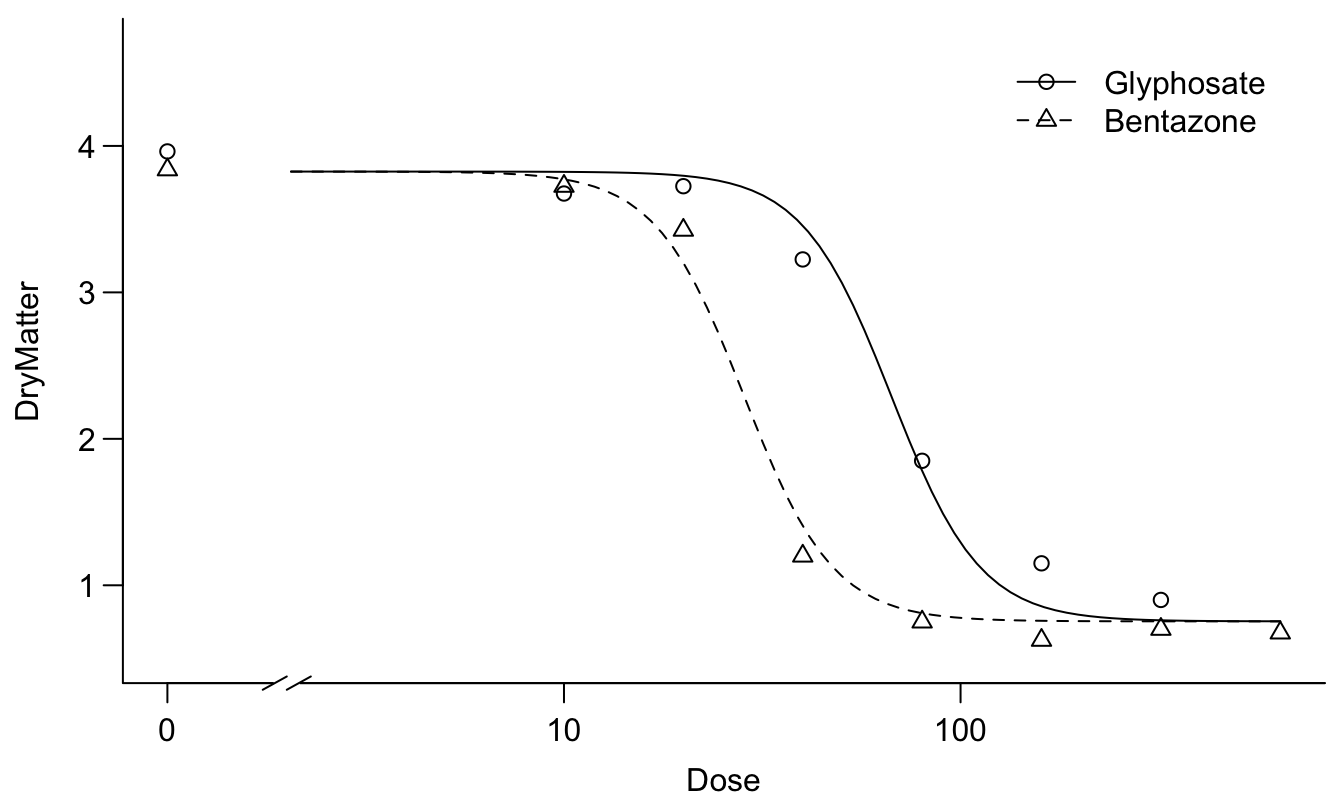
\includegraphics{Rstats4ag_files/figure-latex/figglybentslope-1.pdf}
\caption{\label{fig:figglybentslope}\emph{The two curves are similar except for their relative displacement on the x-axis - this is often called a parallel slopes model.}}
\end{figure}

Comparing Figures \ref{fig:figglybentnlin} and \ref{fig:figglybentslope} shows that the fits are forced so they do not capture the responses properly at the lower limits. As seen below the relative potency with common upper and lower limit but different slopes yield different relative potencies: \(ED_{10}\), \(ED_{50}\), and \(ED_{90}\).

\begin{Shaded}
\begin{Highlighting}[]
\CommentTok{#EDcomp(S.alba.LL.4.1, c(10, 50, 50), interval = "delta")}
\KeywordTok{EDcomp}\NormalTok{(S.alba.m2, }\KeywordTok{c}\NormalTok{(}\DecValTok{10}\NormalTok{, }\DecValTok{10}\NormalTok{), }\DataTypeTok{interval=}\StringTok{"delta"}\NormalTok{, }\DataTypeTok{reverse=}\OtherTok{TRUE}\NormalTok{)}
\end{Highlighting}
\end{Shaded}

\begin{verbatim}
## 
## Estimated ratios of effect doses
## 
##                            Estimate   Lower   Upper
## Glyphosate/Bentazone:10/10  1.44007 0.81836 2.06177
\end{verbatim}

\begin{Shaded}
\begin{Highlighting}[]
\KeywordTok{EDcomp}\NormalTok{(S.alba.m2, }\KeywordTok{c}\NormalTok{(}\DecValTok{50}\NormalTok{, }\DecValTok{50}\NormalTok{), }\DataTypeTok{interval=}\StringTok{"delta"}\NormalTok{, }\DataTypeTok{reverse=}\OtherTok{TRUE}\NormalTok{)}
\end{Highlighting}
\end{Shaded}

\begin{verbatim}
## 
## Estimated ratios of effect doses
## 
##                            Estimate  Lower  Upper
## Glyphosate/Bentazone:50/50   2.3362 1.8571 2.8153
\end{verbatim}

\begin{Shaded}
\begin{Highlighting}[]
\KeywordTok{EDcomp}\NormalTok{(S.alba.m2, }\KeywordTok{c}\NormalTok{(}\DecValTok{90}\NormalTok{, }\DecValTok{90}\NormalTok{), }\DataTypeTok{interval=}\StringTok{"delta"}\NormalTok{, }\DataTypeTok{reverse=}\OtherTok{TRUE}\NormalTok{)}
\end{Highlighting}
\end{Shaded}

\begin{verbatim}
## 
## Estimated ratios of effect doses
## 
##                            Estimate  Lower  Upper
## Glyphosate/Bentazone:90/90   3.7899 2.0793 5.5006
\end{verbatim}

It is noted above that the relative potency varies depending of the ED-level. This is of course due to the fact that the two curves have different slopes, \texttt{b} parameters. From a biological point of view the herbicides have different mode of action and experience shows that contact PS II herbicides, such as bentazon, would have a steeper slope than does the EPSP inhibitor, glyphosate.

In \texttt{drc} there is a function \texttt{relpot()} that can illustrate the relationship between changes of the relative potency and the predicted responses.



\begin{Shaded}
\begin{Highlighting}[]
\KeywordTok{par}\NormalTok{(}\DataTypeTok{mfrow=}\KeywordTok{c}\NormalTok{(}\DecValTok{1}\NormalTok{,}\DecValTok{1}\NormalTok{), }\DataTypeTok{mar=}\KeywordTok{c}\NormalTok{(}\FloatTok{3.2}\NormalTok{,}\FloatTok{3.2}\NormalTok{,.}\DecValTok{5}\NormalTok{,.}\DecValTok{5}\NormalTok{), }\DataTypeTok{mgp=}\KeywordTok{c}\NormalTok{(}\DecValTok{2}\NormalTok{,.}\DecValTok{7}\NormalTok{,}\DecValTok{0}\NormalTok{))}
\KeywordTok{relpot}\NormalTok{(S.alba.m2, }\DataTypeTok{interval =} \StringTok{"delta"}\NormalTok{, }\DataTypeTok{bty=}\StringTok{"l"}\NormalTok{)}
\end{Highlighting}
\end{Shaded}

\begin{figure}
\centering
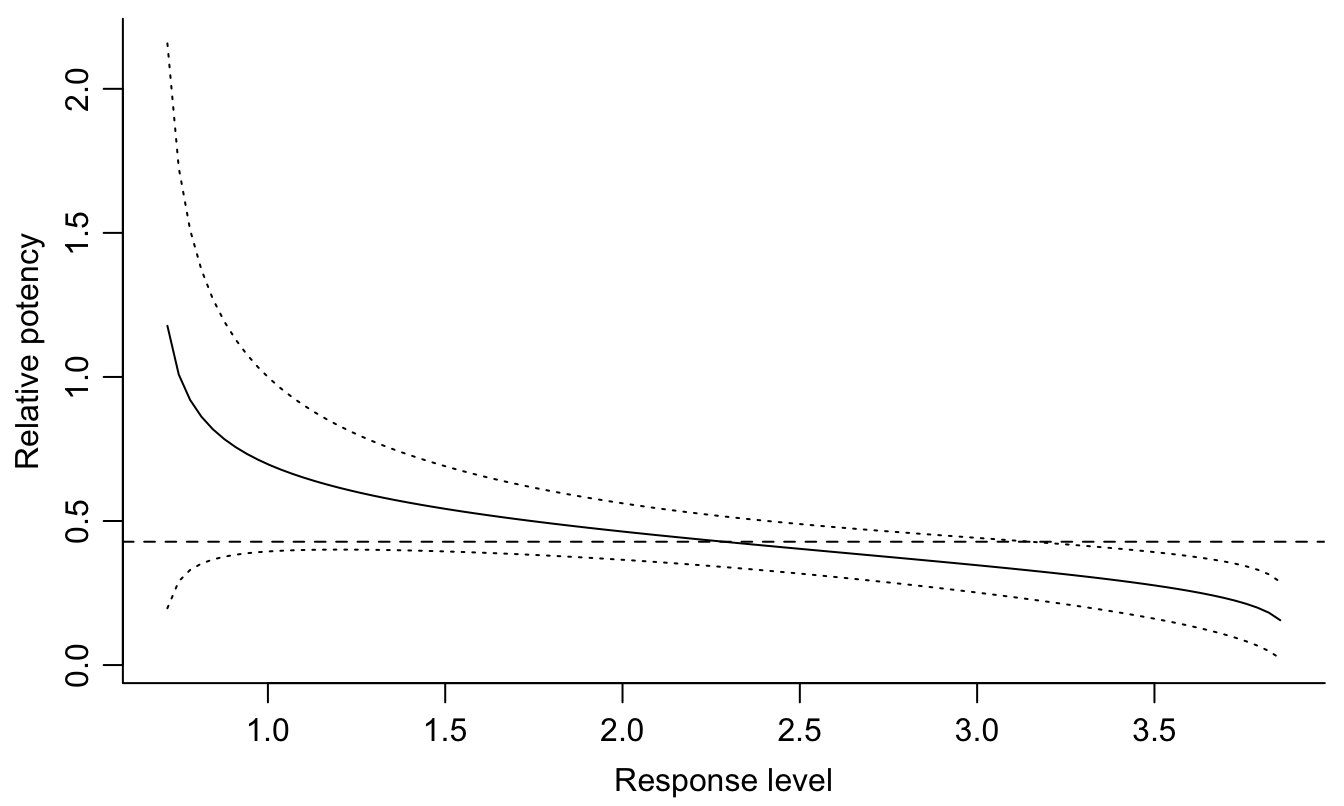
\includegraphics{Rstats4ag_files/figure-latex/figglybenrelpot-1.pdf}
\caption{\label{fig:figglybenrelpot}\emph{The relative potency varies depending of response level, with the 95\% confidence intervals. The dashed horizontal line shows the relative potency at the \(ED_{50}\) for glyphosate and bentazon.}}
\end{figure}

The most precise ED-level is at the \(ED_{50}\); towards the extremes close to the upper and lower limit the variation becomes huge. This is a general trend and explains why we often wish to quantify toxicity of a compound by using \(ED_{50}\).

\hypertarget{when-upper-and-lower-limits-are-not-similar}{%
\section{When Upper and Lower Limits are not similar}\label{when-upper-and-lower-limits-are-not-similar}}

In real life, e.g., when testing herbicide tolerant/resistant biotypes of weeds and different weed species, we cannot expect that the upper and lower limits are similar among curves and that the curves have the same slopes. On the contrary, if there is a penalty for acquiring resistance (fitness cost) then the untreated control for each biotype would be expected to have different biomass. Depending on the time from spraying and ambient growth condition at harvest; the lower limit may also differ.

Whatever the purpose of assessing potencies among plants the problem of different upper and lower limits is often ``solved'' in the literature by scaling the raw data to percentage of untreated control. This ``solution'' often results in smaller but incorrect standard error of \(ED_{50}\) being inflated by the scaling.

In general, we do not want to go for low standard error, but go for the \emph{correct} standard error. Therefore, we recommend to do all the curve-fitting on original raw data!

Below we have two accessions of \emph{Echonichlora oryzoides} where both the upper limit and the lower limits are different.



\begin{Shaded}
\begin{Highlighting}[]
\NormalTok{op <-}\StringTok{ }\KeywordTok{par}\NormalTok{(}\DataTypeTok{mfrow =} \KeywordTok{c}\NormalTok{(}\DecValTok{1}\NormalTok{, }\DecValTok{1}\NormalTok{), }\DataTypeTok{mar=}\KeywordTok{c}\NormalTok{(}\FloatTok{3.2}\NormalTok{,}\FloatTok{3.2}\NormalTok{,.}\DecValTok{5}\NormalTok{,.}\DecValTok{5}\NormalTok{), }\DataTypeTok{mgp=}\KeywordTok{c}\NormalTok{(}\DecValTok{2}\NormalTok{,.}\DecValTok{7}\NormalTok{,}\DecValTok{0}\NormalTok{))}
\NormalTok{TwoCurves<-}\KeywordTok{read.csv}\NormalTok{(}\StringTok{"http://rstats4ag.org/data/twoCurves.csv"}\NormalTok{)}
\KeywordTok{head}\NormalTok{(TwoCurves,}\DecValTok{3}\NormalTok{)}
\end{Highlighting}
\end{Shaded}

\begin{verbatim}
##   xn Dose Accesion Dry.weight.per.pot  X
## 1 33    0  SAM-E-8              1.968 NA
## 2 34    0  SAM-E-8              2.030 NA
## 3 35    0  SAM-E-8              2.129 NA
\end{verbatim}

\begin{Shaded}
\begin{Highlighting}[]
\NormalTok{Bispyribac.sodium.m1 <-}\StringTok{ }\KeywordTok{drm}\NormalTok{(Dry.weight.per.pot }\OperatorTok{~}\StringTok{ }\NormalTok{Dose, Accesion,}
                            \DataTypeTok{data =}\NormalTok{ TwoCurves, }\DataTypeTok{fct=}\KeywordTok{LL.4}\NormalTok{())}
\KeywordTok{modelFit}\NormalTok{(Bispyribac.sodium.m1)}
\end{Highlighting}
\end{Shaded}

\begin{verbatim}
## Lack-of-fit test
## 
##           ModelDf    RSS Df F value p value
## ANOVA          48 1.7678                   
## DRC model      56 2.2799  8  1.7384  0.1137
\end{verbatim}

\begin{Shaded}
\begin{Highlighting}[]
\KeywordTok{summary}\NormalTok{(Bispyribac.sodium.m1)}
\end{Highlighting}
\end{Shaded}

\begin{verbatim}
## 
## Model fitted: Log-logistic (ED50 as parameter) (4 parms)
## 
## Parameter estimates:
## 
##             Estimate Std. Error t-value   p-value    
## b:SAM-E-8   2.047171   0.327585  6.2493 5.957e-08 ***
## b:TEK-E-10  0.876716   0.315014  2.7831  0.007327 ** 
## c:SAM-E-8   0.245913   0.073938  3.3259  0.001560 ** 
## c:TEK-E-10 -0.053077   0.091626 -0.5793  0.564726    
## d:SAM-E-8   2.242014   0.081575 27.4841 < 2.2e-16 ***
## d:TEK-E-10  1.827553   0.101102 18.0764 < 2.2e-16 ***
## e:SAM-E-8  21.702693   2.276642  9.5328 2.514e-13 ***
## e:TEK-E-10  2.666463   1.026905  2.5966  0.012004 *  
## ---
## Signif. codes:  0 '***' 0.001 '**' 0.01 '*' 0.05 '.' 0.1 ' ' 1
## 
## Residual standard error:
## 
##  0.2017751 (56 degrees of freedom)
\end{verbatim}

\begin{Shaded}
\begin{Highlighting}[]
\KeywordTok{plot}\NormalTok{(Bispyribac.sodium.m1, }\DataTypeTok{broken=}\OtherTok{TRUE}\NormalTok{, }\DataTypeTok{bp=}\NormalTok{.}\DecValTok{1}\NormalTok{, }\DataTypeTok{ylab=}\StringTok{"Dry Matter(g/pot)"}\NormalTok{,}
     \DataTypeTok{xlab=}\StringTok{"Bispyribac sodium (g/ha)"}\NormalTok{, }\DataTypeTok{bty=}\StringTok{"l"}\NormalTok{)}

\CommentTok{# drawing lines on the plot}
\NormalTok{ED.SAM.E}\FloatTok{.8}\NormalTok{ <-}\StringTok{ }\FloatTok{0.24591} \OperatorTok{+}\StringTok{ }\NormalTok{(}\FloatTok{2.24201} \OperatorTok{-}\StringTok{ }\FloatTok{0.24591}\NormalTok{) }\OperatorTok{*}\StringTok{ }\FloatTok{0.5}
\NormalTok{ED.TEK.E}\FloatTok{.10}\NormalTok{ <-}\StringTok{ }\FloatTok{-0.05308} \OperatorTok{+}\StringTok{ }\NormalTok{(}\FloatTok{1.82755} \OperatorTok{+-}\StringTok{ }\FloatTok{0.05308}\NormalTok{) }\OperatorTok{*}\StringTok{ }\FloatTok{0.5}
\KeywordTok{arrows}\NormalTok{(}\FloatTok{0.1}\NormalTok{, ED.SAM.E}\FloatTok{.8}\NormalTok{, }\FloatTok{21.7}\NormalTok{, ED.SAM.E}\FloatTok{.8}\NormalTok{, }\DataTypeTok{code=}\DecValTok{0}\NormalTok{)}
\KeywordTok{arrows}\NormalTok{(}\FloatTok{21.7}\NormalTok{, ED.SAM.E}\FloatTok{.8}\NormalTok{, }\FloatTok{21.7}\NormalTok{, }\DecValTok{0}\NormalTok{, }\DataTypeTok{code=}\DecValTok{0}\NormalTok{)}
\KeywordTok{arrows}\NormalTok{(}\FloatTok{0.1}\NormalTok{, ED.TEK.E}\FloatTok{.10}\NormalTok{, }\FloatTok{2.67}\NormalTok{, ED.TEK.E}\FloatTok{.10}\NormalTok{, }\DataTypeTok{code=}\DecValTok{0}\NormalTok{, }\DataTypeTok{lty=}\DecValTok{2}\NormalTok{)}
\KeywordTok{arrows}\NormalTok{(}\FloatTok{2.67}\NormalTok{, ED.TEK.E}\FloatTok{.10}\NormalTok{, }\FloatTok{2.67}\NormalTok{, }\DecValTok{0}\NormalTok{, }\DataTypeTok{code=}\DecValTok{0}\NormalTok{, }\DataTypeTok{lty=}\DecValTok{2}\NormalTok{)}
\end{Highlighting}
\end{Shaded}

\begin{figure}
\centering
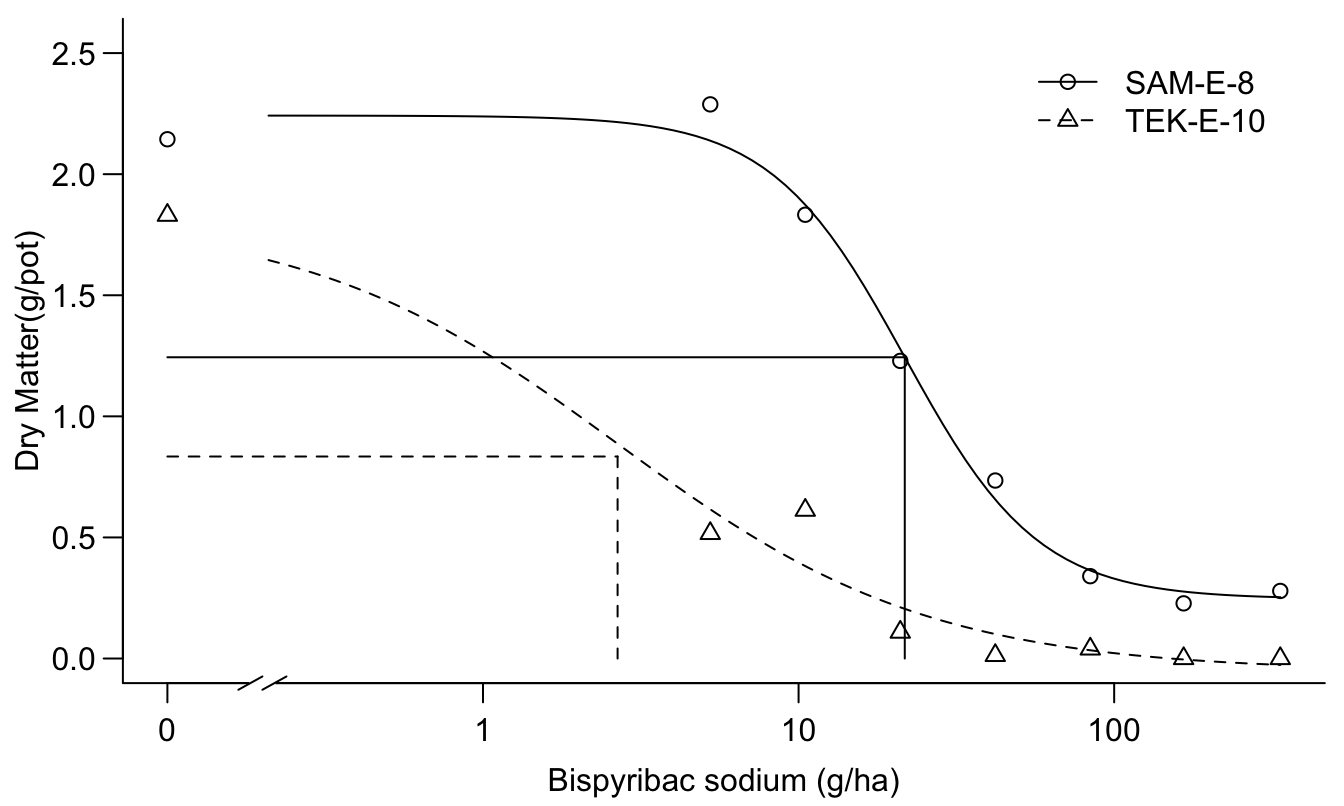
\includegraphics{Rstats4ag_files/figure-latex/figbisrs-1.pdf}
\caption{\label{fig:figbisrs}\emph{Fit of regression for two accessions.}}
\end{figure}

The fit looks reasonable and the test for lack of fit is non-significant and the \(ED_{50}\)s are shown. Everything seems to be all right, but we notice that distribution of observations for TEK-E-10 could be better to describe the mid range of the responses. The summary above reveals that the lower limit, \texttt{c}, for TEK-E-10 is less than zero, not much and not different from zero though, but still illogical. We can re-fit the model using the \texttt{lowerl=} argument which will allow us to restrict model parameters to biologically relevant estimates. In this case, we will restrict the lower limit to values of zero or greater. All other parameters will still be allowed to vary without restriction.

\begin{Shaded}
\begin{Highlighting}[]
\NormalTok{Bispyribac.sodium.m2 <-}\StringTok{ }\KeywordTok{drm}\NormalTok{(Dry.weight.per.pot }\OperatorTok{~}\StringTok{ }\NormalTok{Dose, Accesion,}
                            \DataTypeTok{data =}\NormalTok{ TwoCurves, }\DataTypeTok{fct=}\KeywordTok{LL.4}\NormalTok{(),}
                            \DataTypeTok{lowerl=}\KeywordTok{c}\NormalTok{(}\OtherTok{NA}\NormalTok{,}\DecValTok{0}\NormalTok{,}\OtherTok{NA}\NormalTok{,}\OtherTok{NA}\NormalTok{))}
\KeywordTok{summary}\NormalTok{(Bispyribac.sodium.m2)}
\end{Highlighting}
\end{Shaded}

\begin{verbatim}
## 
## Model fitted: Log-logistic (ED50 as parameter) (4 parms)
## 
## Parameter estimates:
## 
##             Estimate Std. Error t-value   p-value    
## b:SAM-E-8   2.042454   0.329052  6.2071 6.984e-08 ***
## b:TEK-E-10  1.015226   0.313919  3.2340  0.002049 ** 
## c:SAM-E-8   0.243411   0.074596  3.2631  0.001881 ** 
## c:TEK-E-10  0.000000   0.071617  0.0000  1.000000    
## d:SAM-E-8   2.242077   0.082057 27.3234 < 2.2e-16 ***
## d:TEK-E-10  1.826855   0.101703 17.9627 < 2.2e-16 ***
## e:SAM-E-8  21.740911   2.295727  9.4702 3.166e-13 ***
## e:TEK-E-10  2.730186   0.961385  2.8398  0.006280 ** 
## ---
## Signif. codes:  0 '***' 0.001 '**' 0.01 '*' 0.05 '.' 0.1 ' ' 1
## 
## Residual standard error:
## 
##  0.2028892 (56 degrees of freedom)
\end{verbatim}

We see that the standard error dropped and now we will use the fit and calculate the selectivity factor at \(ED_{50}\):

\begin{Shaded}
\begin{Highlighting}[]
\KeywordTok{EDcomp}\NormalTok{(Bispyribac.sodium.m2, }\KeywordTok{c}\NormalTok{(}\DecValTok{50}\NormalTok{, }\DecValTok{50}\NormalTok{),}\DataTypeTok{interval=}\StringTok{"delta"}\NormalTok{)}
\end{Highlighting}
\end{Shaded}

\begin{verbatim}
## 
## Estimated ratios of effect doses
## 
##                        Estimate   Lower   Upper
## SAM-E-8/TEK-E-10:50/50   7.9632  2.0988 13.8275
\end{verbatim}

The resistance factor is about 8 and significantly greater than 1. Note this is one of the few times we do not test the null hypothesis but the hypothesis, that the potency is the same for the two accessions; that is, the relative potency is 1.0. Another important issue is that the dry matter for the \(ED_{50}\) differs because of the different upper and lower limits. This will not be solved by scaling the observation to the individual accessions' untreated control.

Obviously, the \(ED_{50}\) is not at the same response level, and the relative potency of 8 is significantly different form 1.00.

When using absolute dry matter of say 1.24, the response at \(ED_{50}\) for SAM-E-8 and TEK-E-10 is seen below.

\begin{Shaded}
\begin{Highlighting}[]
\KeywordTok{ED}\NormalTok{(Bispyribac.sodium.m2, }\FloatTok{1.24}\NormalTok{, }\DataTypeTok{type=}\StringTok{"absolute"}\NormalTok{, }\DataTypeTok{interval=}\StringTok{"delta"}\NormalTok{)}
\end{Highlighting}
\end{Shaded}

\begin{verbatim}
## 
## Estimated effective doses
## 
##                  Estimate Std. Error     Lower     Upper
## e:SAM-E-8:1.24  21.799437   2.302921 17.186132 26.412741
## e:TEK-E-10:1.24  1.306694   0.698047 -0.091663  2.705051
\end{verbatim}

Looking at the distribution of observation for TEK-E-10, there are no observations to determine the shape of the curve above the \(ED_{50}\).

If this is the right way to compare absolute response level we could use \(ED_{1.24}\) (Figure \ref{fig:figbisrsabs}).



\begin{Shaded}
\begin{Highlighting}[]
\KeywordTok{par}\NormalTok{(}\DataTypeTok{mfrow =} \KeywordTok{c}\NormalTok{(}\DecValTok{1}\NormalTok{, }\DecValTok{1}\NormalTok{), }\DataTypeTok{mar=}\KeywordTok{c}\NormalTok{(}\FloatTok{3.2}\NormalTok{,}\FloatTok{3.2}\NormalTok{,.}\DecValTok{5}\NormalTok{,.}\DecValTok{5}\NormalTok{), }\DataTypeTok{mgp=}\KeywordTok{c}\NormalTok{(}\DecValTok{2}\NormalTok{,.}\DecValTok{7}\NormalTok{,}\DecValTok{0}\NormalTok{))}
\KeywordTok{plot}\NormalTok{(Bispyribac.sodium.m2, }\DataTypeTok{broken=}\OtherTok{TRUE}\NormalTok{, }\DataTypeTok{bp=}\NormalTok{.}\DecValTok{1}\NormalTok{, }\DataTypeTok{bty=}\StringTok{"l"}\NormalTok{,}
     \DataTypeTok{ylab=}\StringTok{"g Dry Matter/pot"}\NormalTok{,}
     \DataTypeTok{xlab=}\StringTok{"Dose (g Bispyribac sodium/ha)"}\NormalTok{)}
\KeywordTok{arrows}\NormalTok{(  }\FloatTok{0.1}\NormalTok{, }\FloatTok{1.24}\NormalTok{, }\FloatTok{21.79}\NormalTok{, }\FloatTok{1.24}\NormalTok{, }\DataTypeTok{code=}\DecValTok{0}\NormalTok{, }\DataTypeTok{lty=}\DecValTok{1}\NormalTok{, }\DataTypeTok{col=}\StringTok{"red"}\NormalTok{)}
\KeywordTok{arrows}\NormalTok{(}\FloatTok{21.79}\NormalTok{, }\FloatTok{1.24}\NormalTok{, }\FloatTok{21.79}\NormalTok{,    }\DecValTok{0}\NormalTok{, }\DataTypeTok{code=}\DecValTok{0}\NormalTok{, }\DataTypeTok{lty=}\DecValTok{1}\NormalTok{, }\DataTypeTok{col=}\StringTok{"red"}\NormalTok{)}
\KeywordTok{arrows}\NormalTok{(  }\FloatTok{1.31}\NormalTok{, }\FloatTok{1.24}\NormalTok{,   }\FloatTok{1.31}\NormalTok{,    }\DecValTok{0}\NormalTok{, }\DataTypeTok{code=}\DecValTok{0}\NormalTok{, }\DataTypeTok{lty=}\DecValTok{2}\NormalTok{, }\DataTypeTok{col=}\StringTok{"red"}\NormalTok{)}
\end{Highlighting}
\end{Shaded}

\begin{figure}
\centering
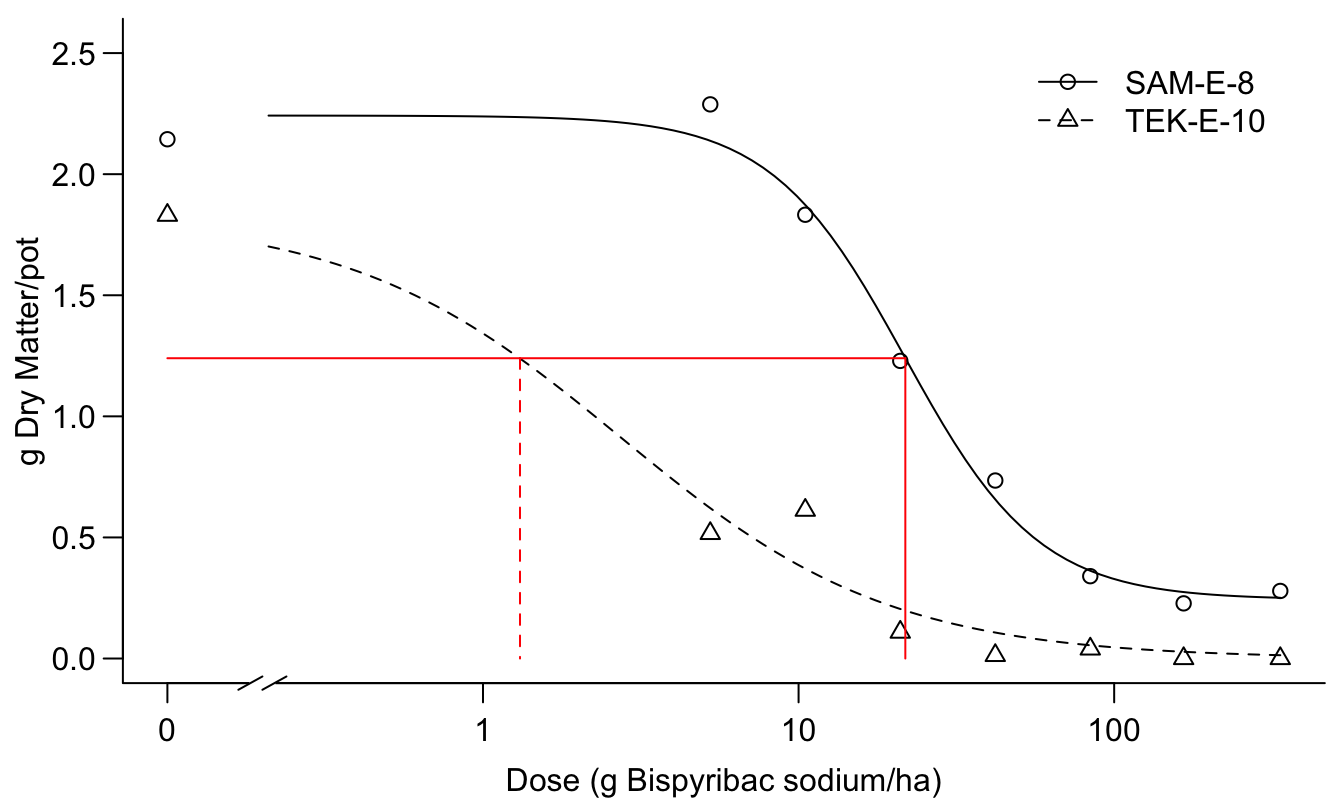
\includegraphics{Rstats4ag_files/figure-latex/figbisrsabs-1.pdf}
\caption{\label{fig:figbisrsabs}\emph{Comparison of the two dose-response curves; red vertical lines show the dose of bispyribac sodium resulting in 1.24 g of dry matter (horizontal line) for the two biotypes.}}
\end{figure}

Now the resistance factor below becomes huge, but so does the confidence interval and consequently the resistance factor is not statistically different from 1.0 at an alpha ov 0.05. The villain is the poor precision of TEK-E-10 \(ED_{1.24}\) that is not significantly different form 0.0.

\begin{Shaded}
\begin{Highlighting}[]
\KeywordTok{EDcomp}\NormalTok{(Bispyribac.sodium.m2, }\KeywordTok{c}\NormalTok{(}\FloatTok{1.24}\NormalTok{, }\FloatTok{1.24}\NormalTok{), }\DataTypeTok{type=}\StringTok{"absolute"}\NormalTok{,}\DataTypeTok{interval=}\StringTok{"delta"}\NormalTok{)}
\end{Highlighting}
\end{Shaded}

\begin{verbatim}
## 
## Estimated ratios of effect doses
## 
##                            Estimate  Lower  Upper
## SAM-E-8/TEK-E-10:1.24/1.24   16.683 -1.516 34.882
\end{verbatim}

The problems described above is virtually never mentioned in the weed science journals, even though it is instrumental to understand what we actually compare. The researcher must choose, and the choice has nothing to do with statistics but with biology.

On the basis of the fit above we can actually scale data on the basis of the regression parameters of the \texttt{d} and the \texttt{c} parameters.



\begin{Shaded}
\begin{Highlighting}[]
\NormalTok{SAM.E.}\FloatTok{8.}\NormalTok{C<-}\KeywordTok{coef}\NormalTok{(Bispyribac.sodium.m1)[}\DecValTok{3}\NormalTok{]}
\NormalTok{TEK.E.}\FloatTok{10.}\NormalTok{C<-}\KeywordTok{coef}\NormalTok{(Bispyribac.sodium.m1)[}\DecValTok{4}\NormalTok{]}
\NormalTok{SAM.E.}\FloatTok{8.}\NormalTok{d<-}\KeywordTok{coef}\NormalTok{(Bispyribac.sodium.m1)[}\DecValTok{5}\NormalTok{]}
\NormalTok{TEK.E.}\FloatTok{10.}\NormalTok{d<-}\KeywordTok{coef}\NormalTok{(Bispyribac.sodium.m1)[}\DecValTok{6}\NormalTok{]}

\NormalTok{Rel.Y<-}\KeywordTok{with}\NormalTok{(TwoCurves,}
            \KeywordTok{ifelse}\NormalTok{(Accesion}\OperatorTok{==}\StringTok{"SAM-E-8"}\NormalTok{, }
\NormalTok{                   ((Dry.weight.per.pot}\OperatorTok{-}\NormalTok{SAM.E.}\FloatTok{8.}\NormalTok{C)}\OperatorTok{/}\NormalTok{(SAM.E.}\FloatTok{8.}\NormalTok{d}\OperatorTok{-}\NormalTok{SAM.E.}\FloatTok{8.}\NormalTok{C)),}
\NormalTok{                   ((Dry.weight.per.pot}\OperatorTok{-}\NormalTok{TEK.E.}\FloatTok{10.}\NormalTok{C)}\OperatorTok{/}\NormalTok{(TEK.E.}\FloatTok{10.}\NormalTok{d}\OperatorTok{-}\NormalTok{TEK.E.}\FloatTok{10.}\NormalTok{C))))}

\NormalTok{Scaled.m1<-}\KeywordTok{drm}\NormalTok{(Rel.Y }\OperatorTok{~}\StringTok{ }\NormalTok{Dose, Accesion, }\DataTypeTok{pmodels=}\KeywordTok{data.frame}\NormalTok{(Accesion, }\DecValTok{1}\NormalTok{, Accesion),}
        \DataTypeTok{data=}\NormalTok{TwoCurves, }\DataTypeTok{fct=}\KeywordTok{LL.3}\NormalTok{())}
\KeywordTok{par}\NormalTok{(}\DataTypeTok{mfrow =} \KeywordTok{c}\NormalTok{(}\DecValTok{1}\NormalTok{, }\DecValTok{1}\NormalTok{), }\DataTypeTok{mar=}\KeywordTok{c}\NormalTok{(}\FloatTok{3.2}\NormalTok{,}\FloatTok{3.2}\NormalTok{,.}\DecValTok{5}\NormalTok{,.}\DecValTok{5}\NormalTok{), }\DataTypeTok{mgp=}\KeywordTok{c}\NormalTok{(}\DecValTok{2}\NormalTok{,.}\DecValTok{7}\NormalTok{,}\DecValTok{0}\NormalTok{))}
\KeywordTok{plot}\NormalTok{(Scaled.m1, }\DataTypeTok{broken=}\OtherTok{TRUE}\NormalTok{, }\DataTypeTok{bp=}\NormalTok{.}\DecValTok{1}\NormalTok{, }\DataTypeTok{bty=}\StringTok{"l"}\NormalTok{, }
     \DataTypeTok{ylab=}\StringTok{"Relative Dry Matter"}\NormalTok{, }\DataTypeTok{ylim=}\KeywordTok{c}\NormalTok{(}\DecValTok{0}\NormalTok{,}\FloatTok{1.2}\NormalTok{),}
     \DataTypeTok{xlab=}\StringTok{"Bispyribac-sodium dose (g/ha)"}\NormalTok{)}
\KeywordTok{arrows}\NormalTok{(  }\FloatTok{0.1}\NormalTok{, }\FloatTok{.5}\NormalTok{, }\FloatTok{21.7}\NormalTok{,.}\DecValTok{5}\NormalTok{, }\DataTypeTok{code=}\DecValTok{0}\NormalTok{, }\DataTypeTok{lty=}\DecValTok{1}\NormalTok{, }\DataTypeTok{col=}\StringTok{"red"}\NormalTok{)}
\KeywordTok{arrows}\NormalTok{(}\FloatTok{21.79}\NormalTok{, }\FloatTok{0.5}\NormalTok{, }\FloatTok{21.79}\NormalTok{,    }\DecValTok{0}\NormalTok{, }\DataTypeTok{code=}\DecValTok{0}\NormalTok{, }\DataTypeTok{lty=}\DecValTok{1}\NormalTok{, }\DataTypeTok{col=}\StringTok{"red"}\NormalTok{)}
\KeywordTok{arrows}\NormalTok{(  }\FloatTok{2.66}\NormalTok{, }\FloatTok{.5}\NormalTok{,   }\FloatTok{2.66}\NormalTok{,    }\DecValTok{0}\NormalTok{, }\DataTypeTok{code=}\DecValTok{0}\NormalTok{, }\DataTypeTok{lty=}\DecValTok{2}\NormalTok{, }\DataTypeTok{col=}\StringTok{"red"}\NormalTok{)}
\end{Highlighting}
\end{Shaded}

\begin{figure}
\centering
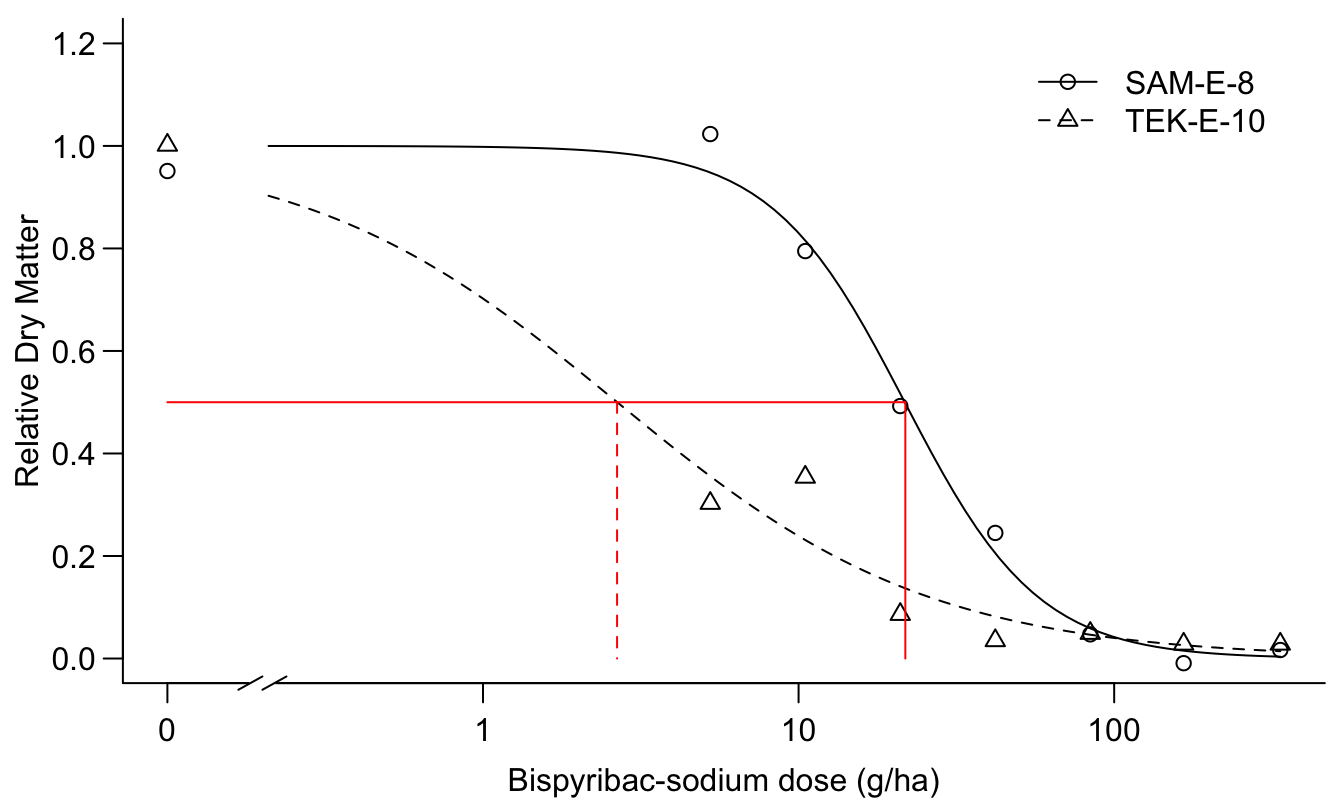
\includegraphics{Rstats4ag_files/figure-latex/figbisrsscaled-1.pdf}
\caption{\label{fig:figbisrsscaled}\emph{Regression fit of scaled responses with similar upper limit, \texttt{d}, and lower limit set to zero.}}
\end{figure}

The summary of the fit in Figure \ref{fig:figbisrsscaled} shows that we get almost the same parameters for the scaled \(ED_{50}\)'s and the selectivity factor is the same but what is concealed by fitting the scaled responses is that the dry matter production is not the same for the two curves, because the scales are originally different. In essence, scaling the data in this way removes the valuable information contained in the \emph{d} parameter without adding benefit.

\begin{Shaded}
\begin{Highlighting}[]
\KeywordTok{summary}\NormalTok{(Scaled.m1)}
\end{Highlighting}
\end{Shaded}

\begin{verbatim}
## 
## Model fitted: Log-logistic (ED50 as parameter) with lower limit at 0 (3 parms)
## 
## Parameter estimates:
## 
##                Estimate Std. Error t-value   p-value    
## b:SAM-E-8      2.048548   0.264669  7.7400 1.507e-10 ***
## b:TEK-E-10     0.875897   0.197672  4.4311 4.133e-05 ***
## d:(Intercept)  0.999972   0.031495 31.7504 < 2.2e-16 ***
## e:SAM-E-8     21.697160   1.825621 11.8848 < 2.2e-16 ***
## e:TEK-E-10     2.662759   0.924541  2.8801  0.005533 ** 
## ---
## Signif. codes:  0 '***' 0.001 '**' 0.01 '*' 0.05 '.' 0.1 ' ' 1
## 
## Residual standard error:
## 
##  0.1005159 (59 degrees of freedom)
\end{verbatim}

\begin{Shaded}
\begin{Highlighting}[]
\KeywordTok{EDcomp}\NormalTok{(Scaled.m1, }\KeywordTok{c}\NormalTok{(}\DecValTok{50}\NormalTok{, }\DecValTok{50}\NormalTok{),}\DataTypeTok{interval=}\StringTok{"delta"}\NormalTok{)}
\end{Highlighting}
\end{Shaded}

\begin{verbatim}
## 
## Estimated ratios of effect doses
## 
##                        Estimate   Lower   Upper
## SAM-E-8/TEK-E-10:50/50   8.1484  2.4492 13.8475
\end{verbatim}

In summary, fitting on raw data the relative potency is 7.96 (2.93) with a coefficient of variation of 37\% with the fit on scaled data on the basis of the upper limits of the regression fit on raw data the relative potency also is 8.14 (2.84) with a coefficient of variation of 32\%. In this instance not dramatically different, except that for the raw data the relative potency is significantly different from zero on the 2\% level whereas for the fit on relative data it is significant on the 1\% level. However, if we go for an absolute ED at the dry matter of 1.24 the the relative potency is 16, but not significantly different from zero. In the literature the differences between untreated controls among accessions can be much larger than here.

\hypertarget{remedy-for-heterogeneous-variance}{%
\section{Remedy for heterogeneous variance}\label{remedy-for-heterogeneous-variance}}

Turning back to the ryegrass dataset the plot of the fit with all observations and the residual plot suggest we should do some kind of transformation or weighing. Because the log-logistic relationship is on the original scale, we cannot just make a transformation of response without doing the same on the right hand side of the equation. \texttt{drc} has a function that can do a a BoxCox transform-both-side regression. You can get more information by executing \texttt{?boxcox.drc}.

\begin{itemize}
\tightlist
\item
  Fit the original model
\item
  update the fit with the function boxcox()
\end{itemize}



\begin{Shaded}
\begin{Highlighting}[]
\KeywordTok{par}\NormalTok{(}\DataTypeTok{mfrow =} \KeywordTok{c}\NormalTok{(}\DecValTok{1}\NormalTok{, }\DecValTok{1}\NormalTok{), }\DataTypeTok{mar=}\KeywordTok{c}\NormalTok{(}\FloatTok{3.2}\NormalTok{,}\FloatTok{3.2}\NormalTok{,.}\DecValTok{5}\NormalTok{,.}\DecValTok{5}\NormalTok{), }\DataTypeTok{mgp=}\KeywordTok{c}\NormalTok{(}\DecValTok{2}\NormalTok{,.}\DecValTok{7}\NormalTok{,}\DecValTok{0}\NormalTok{))}
\NormalTok{ryegrass.BX <-}\StringTok{ }\KeywordTok{boxcox}\NormalTok{(ryegrass.m1,}\DataTypeTok{method=}\StringTok{"anova"}\NormalTok{)}
\end{Highlighting}
\end{Shaded}

\begin{figure}
\centering
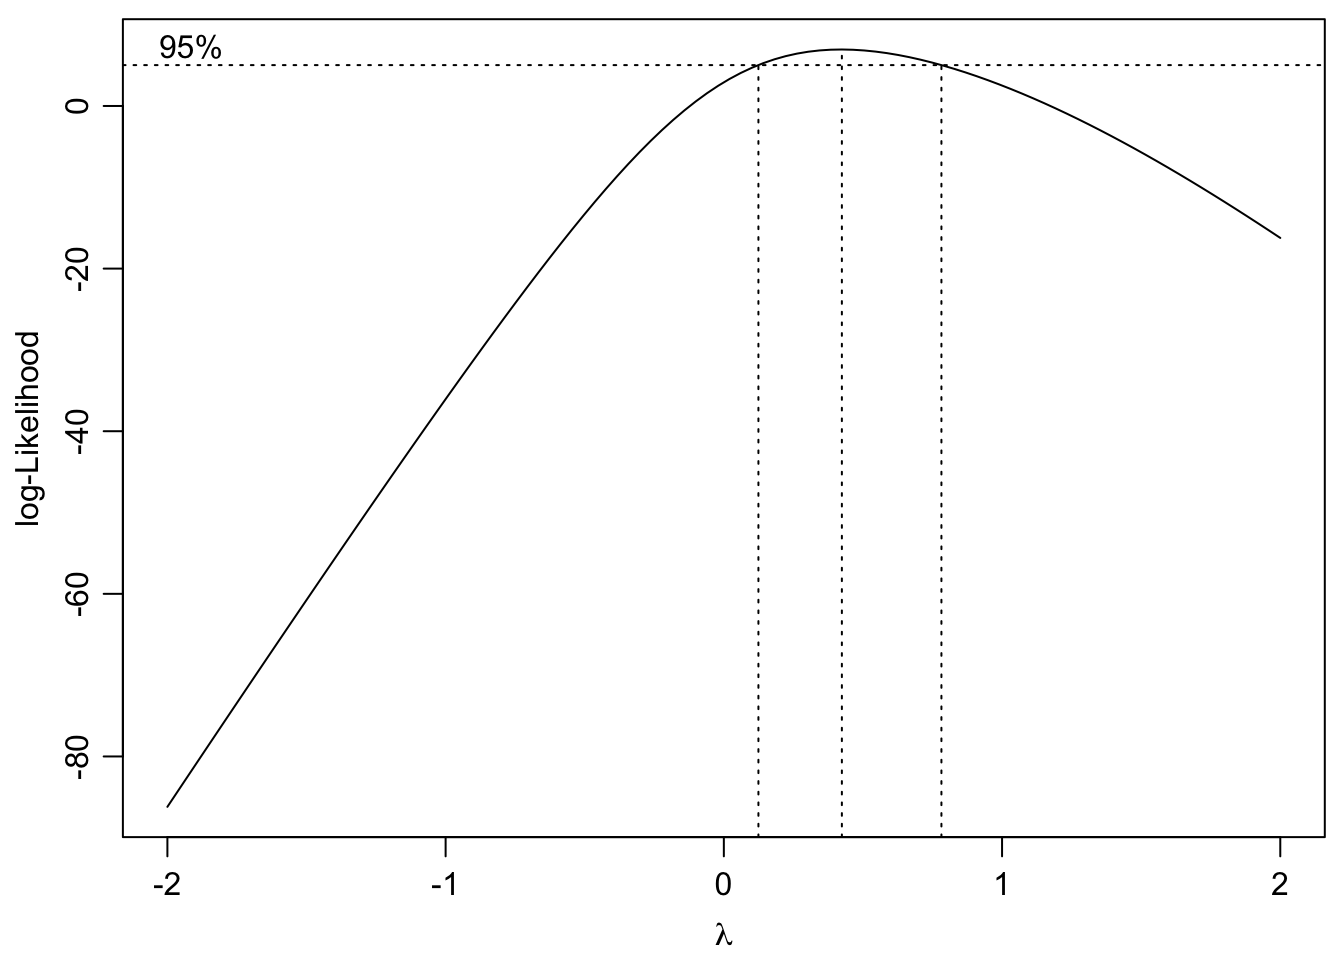
\includegraphics{Rstats4ag_files/figure-latex/figryeboxcox1-1.pdf}
\caption{\label{fig:figryeboxcox1}\emph{Search for optimum \(\lambda\) with confidence intervals. The chosen \(\lambda\) is 0.42.}}
\end{figure}

The summary below give the parameters with the BoxCox transformation.

\begin{Shaded}
\begin{Highlighting}[]
\KeywordTok{summary}\NormalTok{(ryegrass.BX)}
\end{Highlighting}
\end{Shaded}

\begin{verbatim}
## 
## Model fitted: Weibull (type 1) (4 parms)
## 
## Parameter estimates:
## 
##               Estimate Std. Error t-value   p-value    
## b:(Intercept) 1.573865   0.223277  7.0489 7.772e-07 ***
## c:(Intercept) 0.476866   0.090536  5.2672 3.731e-05 ***
## d:(Intercept) 8.007031   0.393446 20.3510 7.759e-15 ***
## e:(Intercept) 3.845926   0.308134 12.4813 6.764e-11 ***
## ---
## Signif. codes:  0 '***' 0.001 '**' 0.01 '*' 0.05 '.' 0.1 ' ' 1
## 
## Residual standard error:
## 
##  0.3258055 (20 degrees of freedom)
## 
## Non-normality/heterogeneity adjustment through optimal Box-Cox transformation
## 
## Estimated lambda: 0.424 
## Confidence interval for lambda: [0.124,0.782]
\end{verbatim}

\begin{Shaded}
\begin{Highlighting}[]
\KeywordTok{ED}\NormalTok{(ryegrass.BX,}\DecValTok{50}\NormalTok{,}\DataTypeTok{interval=}\StringTok{"delta"}\NormalTok{)}
\end{Highlighting}
\end{Shaded}

\begin{verbatim}
## 
## Estimated effective doses
## 
##        Estimate Std. Error   Lower   Upper
## e:1:50  3.04695    0.29106 2.43981 3.65409
\end{verbatim}

The changes in parameters and their standard deviations in relation to the original fit are not dramatic. Normally, if the heterogeneity of variance is moderate and the response curve is well described by responses covering the response range, the changes in the parameters would be small, but perhaps there will be changes in the standard errors. Consequently, if the objective is to compare potency among compounds the prerequisite for constant variance may be important to draw the optimal conclusions.

The residuals after the BoxCox update look a bit better now, compared to the original one.



\begin{Shaded}
\begin{Highlighting}[]
\CommentTok{#Graphical analysis of residuals}
\NormalTok{op <-}\StringTok{ }\KeywordTok{par}\NormalTok{(}\DataTypeTok{mfrow =} \KeywordTok{c}\NormalTok{(}\DecValTok{1}\NormalTok{, }\DecValTok{2}\NormalTok{), }\DataTypeTok{mar=}\KeywordTok{c}\NormalTok{(}\FloatTok{3.2}\NormalTok{,}\FloatTok{3.2}\NormalTok{,}\DecValTok{2}\NormalTok{,.}\DecValTok{5}\NormalTok{), }\DataTypeTok{mgp=}\KeywordTok{c}\NormalTok{(}\DecValTok{2}\NormalTok{,.}\DecValTok{7}\NormalTok{,}\DecValTok{0}\NormalTok{)) }\CommentTok{#put two graphs together}
    \KeywordTok{plot}\NormalTok{(}\KeywordTok{residuals}\NormalTok{(ryegrass.BX) }\OperatorTok{~}\StringTok{ }\KeywordTok{fitted}\NormalTok{(ryegrass.BX), }\DataTypeTok{main=}\StringTok{"Residuals vs Fitted"}\NormalTok{)}
\KeywordTok{abline}\NormalTok{(}\DataTypeTok{h=}\DecValTok{0}\NormalTok{)}
\KeywordTok{qqnorm}\NormalTok{(}\KeywordTok{residuals}\NormalTok{(ryegrass.BX))}
 \KeywordTok{qqline}\NormalTok{(}\KeywordTok{residuals}\NormalTok{(ryegrass.BX))}
\end{Highlighting}
\end{Shaded}

\begin{figure}
\centering
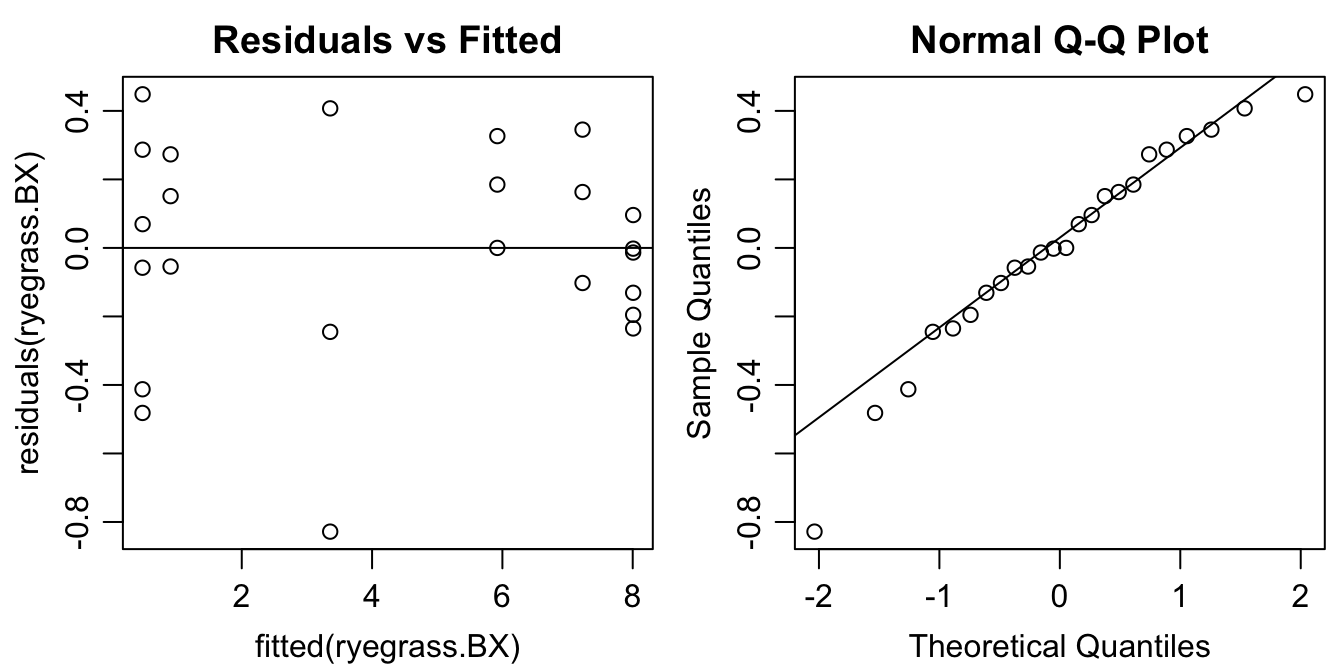
\includegraphics{Rstats4ag_files/figure-latex/figryeboxcoxdiag-1.pdf}
\caption{\label{fig:figryeboxcoxdiag}\emph{Residual plots of BoxCox transformed-both-sides.The funnel type distribution of the residuals now has disappeared.}}
\end{figure}

\hypertarget{dose-responses-with-binomial-data}{%
\section{Dose-responses with binomial data}\label{dose-responses-with-binomial-data}}

Survival of plant or ability to germinate in response to herbicides is a classical underlying construct in toxicology. In weed science it also is important because \emph{the only good weed is a dead weed}. Particularly, in these ages of detecting herbicide resistance/tolerance the dead or alive response is important. In insecticide research and in general toxicology the binomial response, dead or alive or affected not affected is fundamental for classifying toxic compounds.

A prerequisite is that we know how to properly classify the demise of a plant. We are far away from the normal distribution. The data, however, can still be analysed with the function \texttt{drm()} but a new argument must be included in the \texttt{drm()} function, viz \texttt{type="binomial}.

\hypertarget{example-1-herbicide-susceptibility}{%
\subsection{Example 1: Herbicide susceptibility}\label{example-1-herbicide-susceptibility}}

Below we have an experiment with putative glyphosate sensitive and tolerant biotypes of \emph{Chenopodium album} and the survival as response, which takes two values: 0 means dead and 1 means alive. In fact, every plants is an experimental unit. We assume that all plants survived in the untreated control and at infinite high rates all plants die. It is important to note, though, that this assumption may not always hold; for example, some triazine-resistant biotypes may not be killed by atrazine, even at exceptionally high doses. But for this example, the data suggest that even the tolerant biotype can be killed at high doses.



\begin{Shaded}
\begin{Highlighting}[]
\KeywordTok{library}\NormalTok{(drc)}
\KeywordTok{read.csv}\NormalTok{(}\StringTok{"http://rstats4ag.org/data/chealglyph.csv"}\NormalTok{)->cheal.dat}
\KeywordTok{head}\NormalTok{(cheal.dat,}\DataTypeTok{n=}\DecValTok{3}\NormalTok{)}
\end{Highlighting}
\end{Shaded}

\begin{verbatim}
##   block biotype glyph.rate survival
## 1     A       S        426        0
## 2     A       T       1680        0
## 3     A       T          0        1
\end{verbatim}

\begin{Shaded}
\begin{Highlighting}[]
\KeywordTok{drm}\NormalTok{(survival }\OperatorTok{~}\StringTok{ }\NormalTok{glyph.rate, biotype, }\DataTypeTok{fct=}\KeywordTok{LL.2}\NormalTok{(}\DataTypeTok{names=}\KeywordTok{c}\NormalTok{(}\StringTok{"Slope"}\NormalTok{, }\StringTok{"LD50"}\NormalTok{)),}
    \DataTypeTok{type=}\NormalTok{(}\StringTok{"binomial"}\NormalTok{), }\DataTypeTok{data=}\NormalTok{cheal.dat, }\DataTypeTok{na.action=}\NormalTok{na.omit)->cheal.drm}

\KeywordTok{par}\NormalTok{(}\DataTypeTok{mfrow =} \KeywordTok{c}\NormalTok{(}\DecValTok{1}\NormalTok{, }\DecValTok{1}\NormalTok{), }\DataTypeTok{mar=}\KeywordTok{c}\NormalTok{(}\FloatTok{3.2}\NormalTok{,}\FloatTok{3.2}\NormalTok{,.}\DecValTok{5}\NormalTok{,.}\DecValTok{5}\NormalTok{), }\DataTypeTok{mgp=}\KeywordTok{c}\NormalTok{(}\DecValTok{2}\NormalTok{,.}\DecValTok{7}\NormalTok{,}\DecValTok{0}\NormalTok{))}
\KeywordTok{plot}\NormalTok{(cheal.drm, }\DataTypeTok{broken=}\OtherTok{TRUE}\NormalTok{, }\DataTypeTok{xlim=}\KeywordTok{c}\NormalTok{(}\DecValTok{0}\NormalTok{,}\DecValTok{10000}\NormalTok{), }\DataTypeTok{bty=}\StringTok{"l"}\NormalTok{,}
     \DataTypeTok{xlab=}\StringTok{"glyphosate rate"}\NormalTok{, }\DataTypeTok{ylab=}\StringTok{"P(survival)"}\NormalTok{)}
\end{Highlighting}
\end{Shaded}

\begin{figure}
\centering
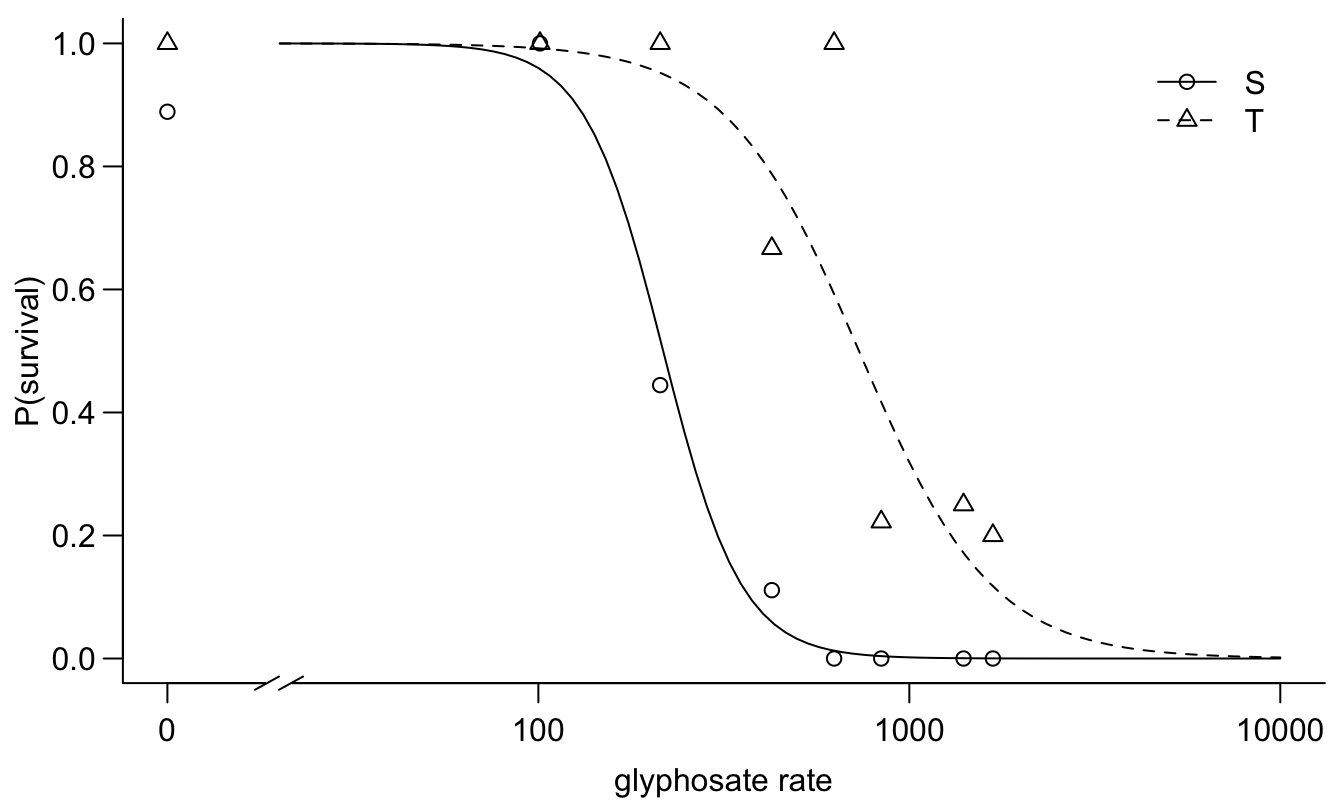
\includegraphics{Rstats4ag_files/figure-latex/figchealst-1.pdf}
\caption{\label{fig:figchealst}\emph{Dose-response curves for survival of} Chenopodium album \emph{classified \textbf{a priori} as either sensitive or tolerant to glyphosate based on field history.}}
\end{figure}

\begin{Shaded}
\begin{Highlighting}[]
\KeywordTok{modelFit}\NormalTok{(cheal.drm)}
\end{Highlighting}
\end{Shaded}

\begin{verbatim}
## Goodness-of-fit test
## 
##             Df Chisq value p value
##                                   
## DRC model   89      63.247  0.9823
\end{verbatim}

\begin{Shaded}
\begin{Highlighting}[]
\KeywordTok{summary}\NormalTok{(cheal.drm)}
\end{Highlighting}
\end{Shaded}

\begin{verbatim}
## 
## Model fitted: Log-logistic (ED50 as parameter) with lower limit at 0 and upper limit at 1 (2 parms)
## 
## Parameter estimates:
## 
##          Estimate Std. Error t-value   p-value    
## Slope:S   4.10418    1.40025  2.9310 0.0033783 ** 
## Slope:T   2.42592    0.72357  3.3527 0.0008003 ***
## LD50:S  216.98961   30.29692  7.1621 7.945e-13 ***
## LD50:T  731.56946  122.16134  5.9886 2.117e-09 ***
## ---
## Signif. codes:  0 '***' 0.001 '**' 0.01 '*' 0.05 '.' 0.1 ' ' 1
\end{verbatim}

The data from the tolerant biotypes are not as `clean' as for the sensitive biotype, and this is reflected in the standard error of the \(LD_{50}\). This variability is often to be expected when a population is still segregating for a resistance trait, and individual organisms are being used as experimental units. The ?EDcomp()` function can be used to test whether the \(LD_{50}\) is statistically different between biotypes.

\begin{Shaded}
\begin{Highlighting}[]
\KeywordTok{EDcomp}\NormalTok{(cheal.drm,}\KeywordTok{c}\NormalTok{(}\DecValTok{50}\NormalTok{,}\DecValTok{50}\NormalTok{), }\DataTypeTok{reverse=}\OtherTok{TRUE}\NormalTok{)}
\end{Highlighting}
\end{Shaded}

\begin{verbatim}
## 
## Estimated ratios of effect doses
## 
##            Estimate Std. Error   t-value   p-value
## T/S:50/50 3.3714492  0.7338531 3.2315040 0.0012314
\end{verbatim}

The two biotypes exhibit an approximately 3-fold difference in susceptibility to glyphosate, and this difference is statistically different from 1.

Another important issue here, is that the response range goes between 0 to 1.0, which is in contrast to the use of continuous response variables such as biomass. Generally, you get more information using biomass or other continuous responses, but also more difficult choices for interpretation, as mentioned before about, e.g.~how to deal with different upper limit and lower limits among dose response curves.

\hypertarget{example-2-earthworm-toxicity}{%
\subsection{Example 2: Earthworm toxicity}\label{example-2-earthworm-toxicity}}

The next example is from an ecotoxicological experiment with earthworms. A number of earthworms is distributed uniformly in a container where one half of the container surface is contaminated by a toxic substance (not disclosed). If the earthworms do not like the substance they will flee to the uncontaminated part of the container.

In this dataset the arrangement for data is somewhat different from the one with the sensitive and tolerant Chenopodium album. For each container we have a dose, a total number of earthworms, and the number of earthworms that migrated away form the contaminated part of the container. Consequently, we now need to use an additional argument in \texttt{drm()}, a weighing argument \texttt{weights=total}.



\begin{Shaded}
\begin{Highlighting}[]
\KeywordTok{head}\NormalTok{(earthworms,}\DataTypeTok{n=}\DecValTok{3}\NormalTok{)}
\end{Highlighting}
\end{Shaded}

\begin{verbatim}
##   dose number total
## 1    0      3     5
## 2    0      3     5
## 3    0      3     4
\end{verbatim}

\begin{Shaded}
\begin{Highlighting}[]
\CommentTok{## Fitting a logistic regression model}
\NormalTok{earthworms.m1 <-}\StringTok{ }\KeywordTok{drm}\NormalTok{(number}\OperatorTok{/}\NormalTok{total }\OperatorTok{~}\StringTok{ }\NormalTok{dose, }\DataTypeTok{weights =}\NormalTok{ total, }\DataTypeTok{data =}\NormalTok{ earthworms,}
                     \DataTypeTok{fct =} \KeywordTok{LL.2}\NormalTok{(), }\DataTypeTok{type =} \StringTok{"binomial"}\NormalTok{)}
\KeywordTok{modelFit}\NormalTok{(earthworms.m1)  }\CommentTok{# a crude goodness-of-fit test}
\end{Highlighting}
\end{Shaded}

\begin{verbatim}
## Goodness-of-fit test
## 
##             Df Chisq value p value
##                                   
## DRC model   28      35.236  0.1631
\end{verbatim}

\begin{Shaded}
\begin{Highlighting}[]
\KeywordTok{summary}\NormalTok{(earthworms.m1)}
\end{Highlighting}
\end{Shaded}

\begin{verbatim}
## 
## Model fitted: Log-logistic (ED50 as parameter) with lower limit at 0 and upper limit at 1 (2 parms)
## 
## Parameter estimates:
## 
##               Estimate Std. Error t-value   p-value    
## b:(Intercept) 1.260321   0.246707  5.1086 3.246e-07 ***
## e:(Intercept) 0.145140   0.036797  3.9444 8.000e-05 ***
## ---
## Signif. codes:  0 '***' 0.001 '**' 0.01 '*' 0.05 '.' 0.1 ' ' 1
\end{verbatim}

\begin{Shaded}
\begin{Highlighting}[]
\KeywordTok{par}\NormalTok{(}\DataTypeTok{mfrow =} \KeywordTok{c}\NormalTok{(}\DecValTok{1}\NormalTok{, }\DecValTok{1}\NormalTok{), }\DataTypeTok{mar=}\KeywordTok{c}\NormalTok{(}\FloatTok{3.2}\NormalTok{,}\FloatTok{3.2}\NormalTok{,.}\DecValTok{5}\NormalTok{,.}\DecValTok{5}\NormalTok{), }\DataTypeTok{mgp=}\KeywordTok{c}\NormalTok{(}\DecValTok{2}\NormalTok{,.}\DecValTok{7}\NormalTok{,}\DecValTok{0}\NormalTok{))}
\KeywordTok{plot}\NormalTok{(earthworms.m1, }\DataTypeTok{broken=}\OtherTok{TRUE}\NormalTok{, }\DataTypeTok{bty=}\StringTok{"l"}\NormalTok{)}
\end{Highlighting}
\end{Shaded}

\begin{figure}
\centering
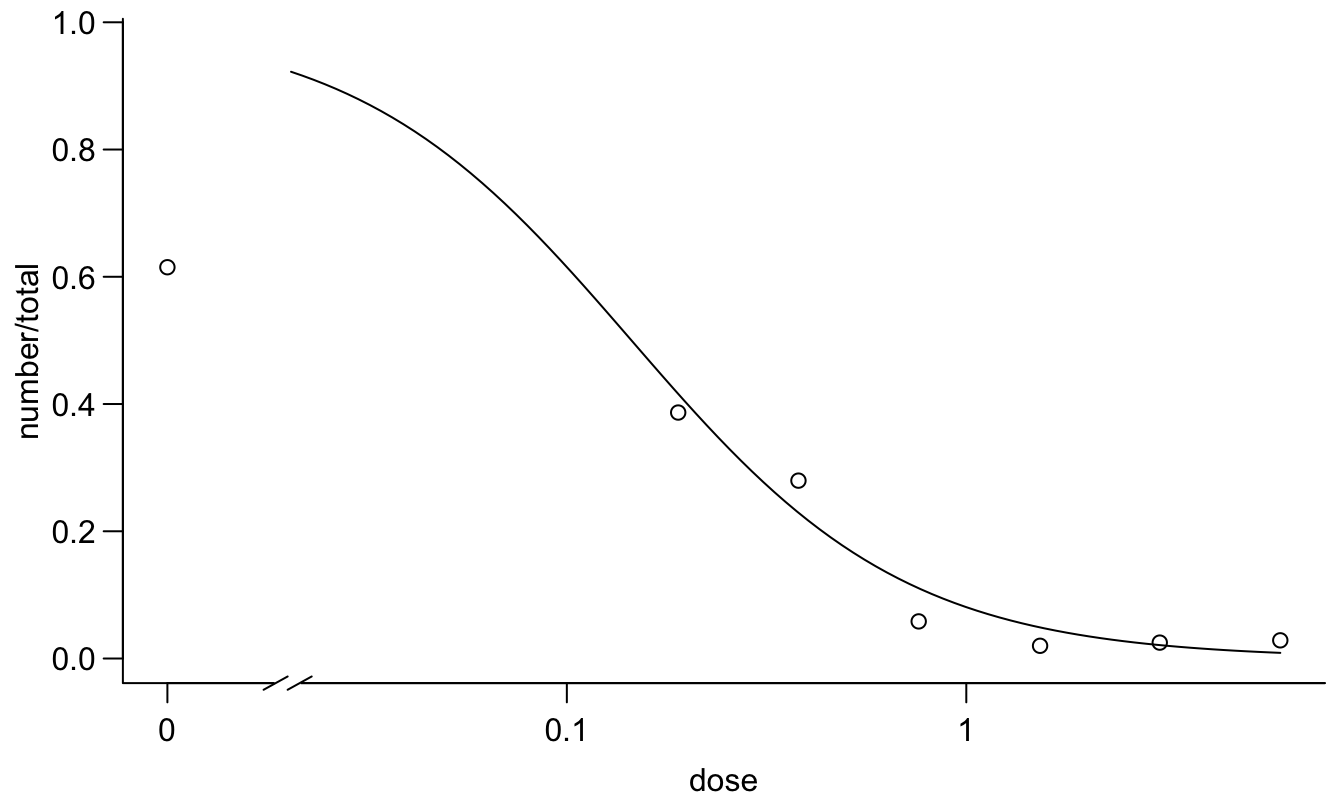
\includegraphics{Rstats4ag_files/figure-latex/figworms10-1.pdf}
\caption{\label{fig:figworms10}\emph{Standard 2 parameter log-logistic dose-response regression with upper and lower limits set to 1 and 0, respectively.}}
\end{figure}

The regression above is a standard the with an upper limit of 1 and apparently the goodness of fit is not significant, even though the untreated control is around 0.6. From a biological point of view the earthworms can move freely after half of the container is contaminated with toxic materials. In the untreated control with no contamination we expect that around 0.5 would be present in the part where we count. Therefore, a 2-parameter model with the upper limit fixed at 1.0 does not seem appropriate here. Consequently, we will introduce a three parameter log-logistic model with an upper limit being estimated on the basis of data.



\begin{Shaded}
\begin{Highlighting}[]
\CommentTok{## Fitting an extended logistic regression model }
\CommentTok{##  where the upper limit is estimated}
\NormalTok{earthworms.m2 <-}\StringTok{ }\KeywordTok{drm}\NormalTok{(number}\OperatorTok{/}\NormalTok{total }\OperatorTok{~}\StringTok{ }\NormalTok{dose, }\DataTypeTok{weights =}\NormalTok{ total, }\DataTypeTok{data =}\NormalTok{ earthworms,}
                     \DataTypeTok{fct =} \KeywordTok{LL.3}\NormalTok{(), }\DataTypeTok{type =} \StringTok{"binomial"}\NormalTok{)}
\KeywordTok{modelFit}\NormalTok{(earthworms.m2)  }\CommentTok{# goodness-of-fit test}
\end{Highlighting}
\end{Shaded}

\begin{verbatim}
## Goodness-of-fit test
## 
##             Df Chisq value p value
##                                   
## DRC model   32       43.13  0.0905
\end{verbatim}

\begin{Shaded}
\begin{Highlighting}[]
\KeywordTok{summary}\NormalTok{(earthworms.m2)}
\end{Highlighting}
\end{Shaded}

\begin{verbatim}
## 
## Model fitted: Log-logistic (ED50 as parameter) with lower limit at 0 (3 parms)
## 
## Parameter estimates:
## 
##               Estimate Std. Error t-value   p-value    
## b:(Intercept) 1.505679   0.338992  4.4416 8.928e-06 ***
## d:(Intercept) 0.604929   0.085800  7.0505 1.783e-12 ***
## e:(Intercept) 0.292428   0.083895  3.4856  0.000491 ***
## ---
## Signif. codes:  0 '***' 0.001 '**' 0.01 '*' 0.05 '.' 0.1 ' ' 1
\end{verbatim}

\begin{Shaded}
\begin{Highlighting}[]
\KeywordTok{par}\NormalTok{(}\DataTypeTok{mfrow =} \KeywordTok{c}\NormalTok{(}\DecValTok{1}\NormalTok{, }\DecValTok{1}\NormalTok{), }\DataTypeTok{mar=}\KeywordTok{c}\NormalTok{(}\FloatTok{3.2}\NormalTok{,}\FloatTok{3.2}\NormalTok{,.}\DecValTok{5}\NormalTok{,.}\DecValTok{5}\NormalTok{), }\DataTypeTok{mgp=}\KeywordTok{c}\NormalTok{(}\DecValTok{2}\NormalTok{,.}\DecValTok{7}\NormalTok{,}\DecValTok{0}\NormalTok{))}
\KeywordTok{plot}\NormalTok{(earthworms.m2, }\DataTypeTok{broken=}\OtherTok{TRUE}\NormalTok{, }\DataTypeTok{bty=}\StringTok{"l"}\NormalTok{)}
\end{Highlighting}
\end{Shaded}

\begin{figure}
\centering
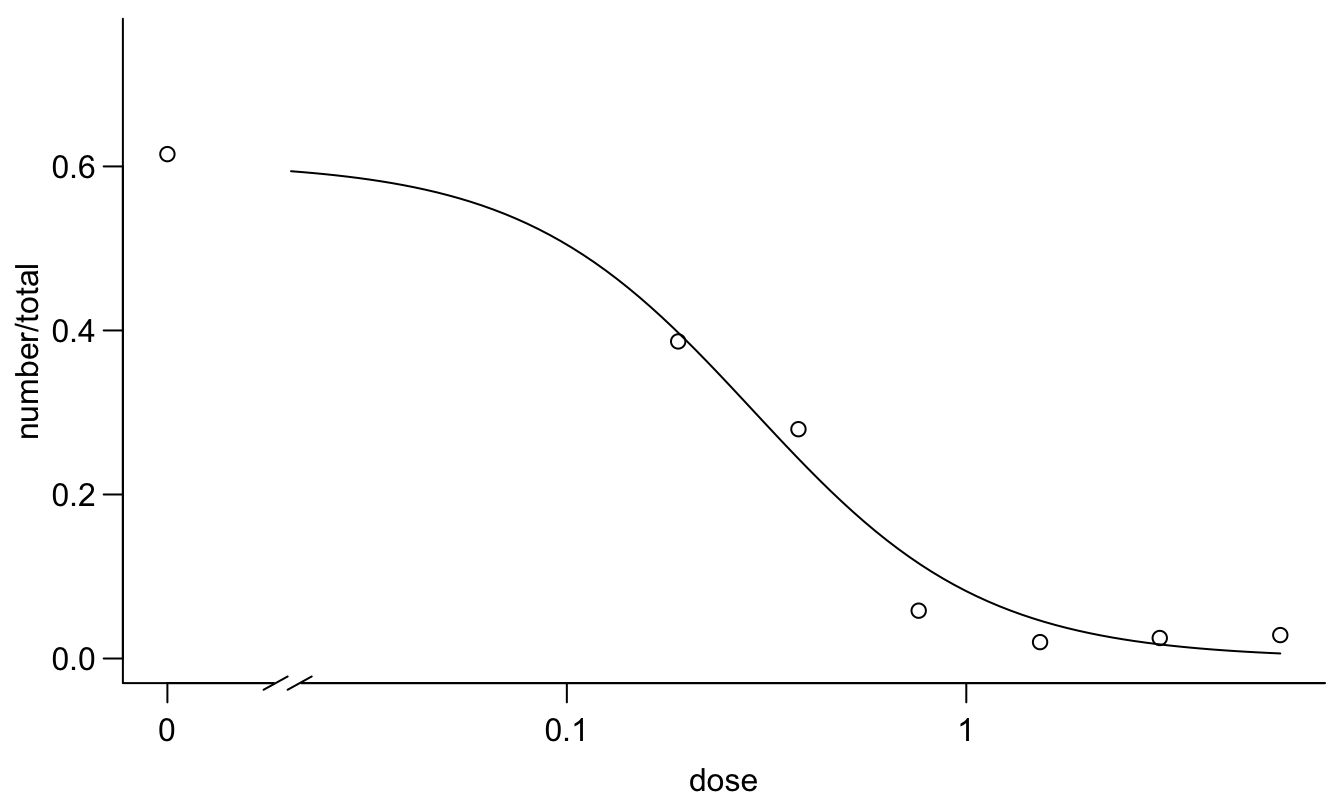
\includegraphics{Rstats4ag_files/figure-latex/figworms0-1.pdf}
\caption{\label{fig:figworms0}\emph{Regression fit with the upper limit being estimated instead of fixed at 1.0.}}
\end{figure}

The goodness of fit was also here acceptable, so on the basis of the statistics we cannot pick the ``best model''. However, we could compare the AIC for the two models and pick the lowest value.

\begin{Shaded}
\begin{Highlighting}[]
\KeywordTok{AIC}\NormalTok{(earthworms.m1, earthworms.m2)}
\end{Highlighting}
\end{Shaded}

\begin{verbatim}
##               df       AIC
## earthworms.m1  2 699.10026
## earthworms.m2  3  78.31036
\end{verbatim}

The model with the estimated upper limit has an AIC that is 9 times smaller than the 2-parameter model. This also corresponds with what we biologically expected.

The \(LD_{50}\) changed somewhat because the upper limit changed, not because there is much difference of the mid part of the curves as snow below.



\begin{Shaded}
\begin{Highlighting}[]
\KeywordTok{par}\NormalTok{(}\DataTypeTok{mfrow =} \KeywordTok{c}\NormalTok{(}\DecValTok{1}\NormalTok{, }\DecValTok{1}\NormalTok{), }\DataTypeTok{mar=}\KeywordTok{c}\NormalTok{(}\FloatTok{3.2}\NormalTok{,}\FloatTok{3.2}\NormalTok{,.}\DecValTok{5}\NormalTok{,.}\DecValTok{5}\NormalTok{), }\DataTypeTok{mgp=}\KeywordTok{c}\NormalTok{(}\DecValTok{2}\NormalTok{,.}\DecValTok{7}\NormalTok{,}\DecValTok{0}\NormalTok{))}
\KeywordTok{plot}\NormalTok{(earthworms.m1, }\DataTypeTok{broken=}\OtherTok{TRUE}\NormalTok{,  }\DataTypeTok{col=}\StringTok{"red"}\NormalTok{, }\DataTypeTok{lty=}\DecValTok{2}\NormalTok{, }\DataTypeTok{bty=}\StringTok{"l"}\NormalTok{)}
\KeywordTok{plot}\NormalTok{(earthworms.m2, }\DataTypeTok{broken=}\OtherTok{TRUE}\NormalTok{, }\DataTypeTok{add=}\OtherTok{TRUE}\NormalTok{)}
\KeywordTok{legend}\NormalTok{(}\StringTok{"topright"}\NormalTok{,}\KeywordTok{c}\NormalTok{(}\StringTok{"2-parameter model (d = 1)"}\NormalTok{, }\StringTok{"3-parameter model (d = estimated)"}\NormalTok{),}
       \DataTypeTok{lty=}\DecValTok{2}\OperatorTok{:}\DecValTok{1}\NormalTok{, }\DataTypeTok{col=}\KeywordTok{c}\NormalTok{(}\StringTok{"red"}\NormalTok{,}\DecValTok{1}\NormalTok{))}
\end{Highlighting}
\end{Shaded}

\begin{figure}
\centering
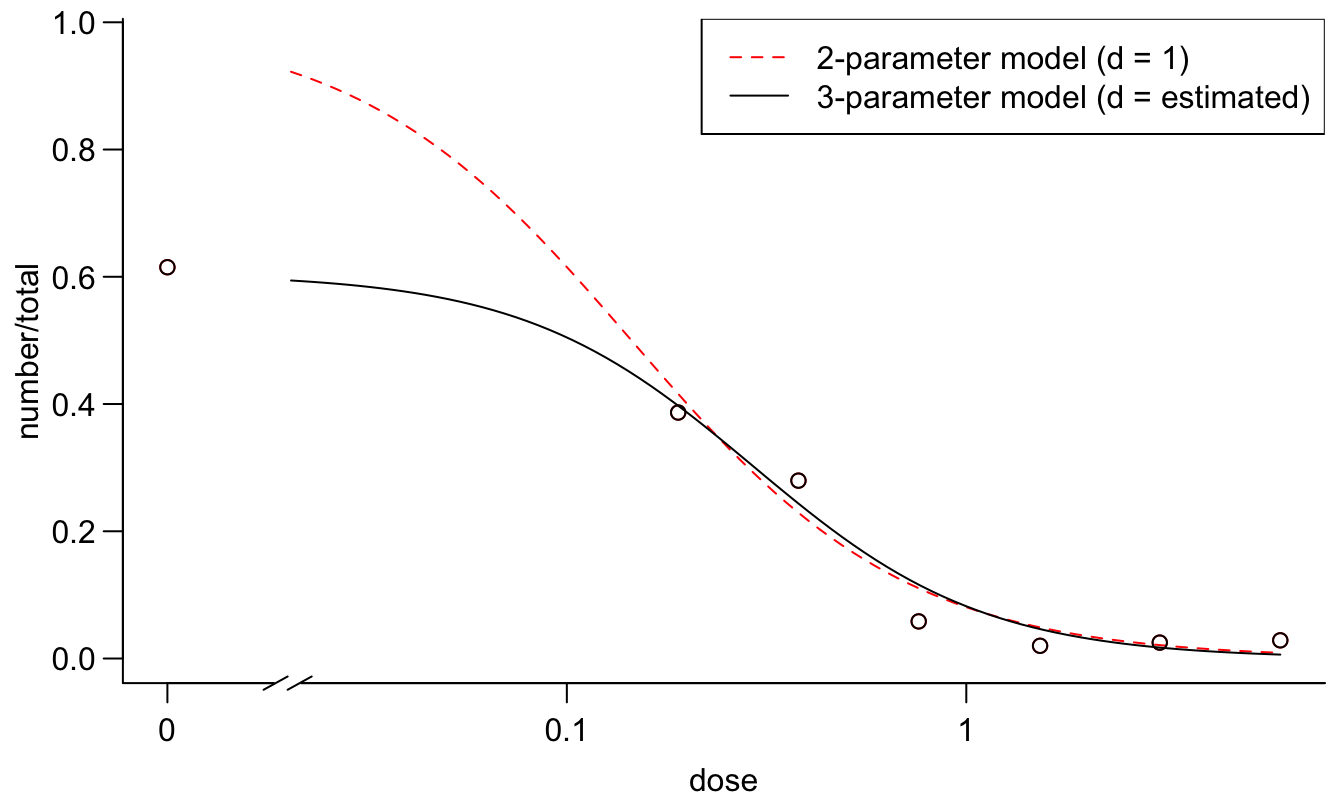
\includegraphics{Rstats4ag_files/figure-latex/figwormsboth-1.pdf}
\caption{\label{fig:figwormsboth}\emph{Comparison between the two curves fittings on with standard \texttt{d}=1 and one with a \texttt{d} determined by data.}}
\end{figure}

The earthworm example is a good one, because the biological knowledge of the set up of the experiment is instrumental to understanding which model to use. In fact the \(LD_{50}\) ranged from 0.04 with the 2 parameter log-logistic fit to 0.29 while the 3 parameter log-logistic fit, which was the correct one from a biological point of view. We do expect that the earthworms would evenly distribute themselves in the untreated control with about 50\% in each part of the box.

\begin{center}\rule{0.5\linewidth}{0.5pt}\end{center}

\hypertarget{nonlinear-regression---selectivity-of-herbicides}{%
\chapter{Nonlinear Regression - Selectivity of Herbicides}\label{nonlinear-regression---selectivity-of-herbicides}}

Herbicides are unique in that they are designed to kill plants. Sufficiently high doses will kill both crops and weeds, while small doses have no effect on crops and weeds. For the selective herbicides there are dose-range windows that control some weeds without harming the crop too much. The action of a herbicide is usually determined by its chemical and physical properties, its effect on plant metabolism, the stage of development of the plant and the environment. The purpose of this chapter is to give an overview of the basic principles of how to quantitatively assess herbicide selectivity.

The chapter is based upon general toxicology commonly used in many disciplines of the biological sciences and it is also used to classify xenobiotics according to their toxic profile; the first of which is the dose required to kill 50\% of some test animals (e.g., rats, mice, hamsters). However, the principles in the pesticide science have focus not only on general toxicity, but also on selectivity, particularly when it comes to herbicides.

\hypertarget{dose-response-curves-1}{%
\section{Dose-Response Curves}\label{dose-response-curves-1}}

The difference between tolerance and control of a plant is determined by the size of the dose. The term size of a dose, however, is rather vague in that for some herbicides, only few g/ha are needed to control weeds (e.g., many sulfonylureas) whereas for others we must apply several kg to obtain the same level of control (e.g., phenoxy acids). If we want to determine the potency or selectivity of a herbicide it is not enough only to look at one dose-response curve, as the proper assessment of selectivity should be stated in relative terms depending on the herbicide, crops and weeds in question. In order to avoid ambiguity in assessment of selectivity the sigmoid log-logistic dose-response curve is a good starting point.

\[y=c+\frac{d-c}{1+ \left(\frac{x}{ED_{50}}\right)^b} \]

Where \texttt{y} is the response, \texttt{d}
denotes the upper limit, \texttt{c} the lower limit, \(ED_{50}\) denotes the dose,
\texttt{x}, required to half the response 50\% between \texttt{d} and \texttt{c}. Finally \texttt{b} denotes the relative slope of the curve around \(ED_{50}\).



\begin{figure}
\centering
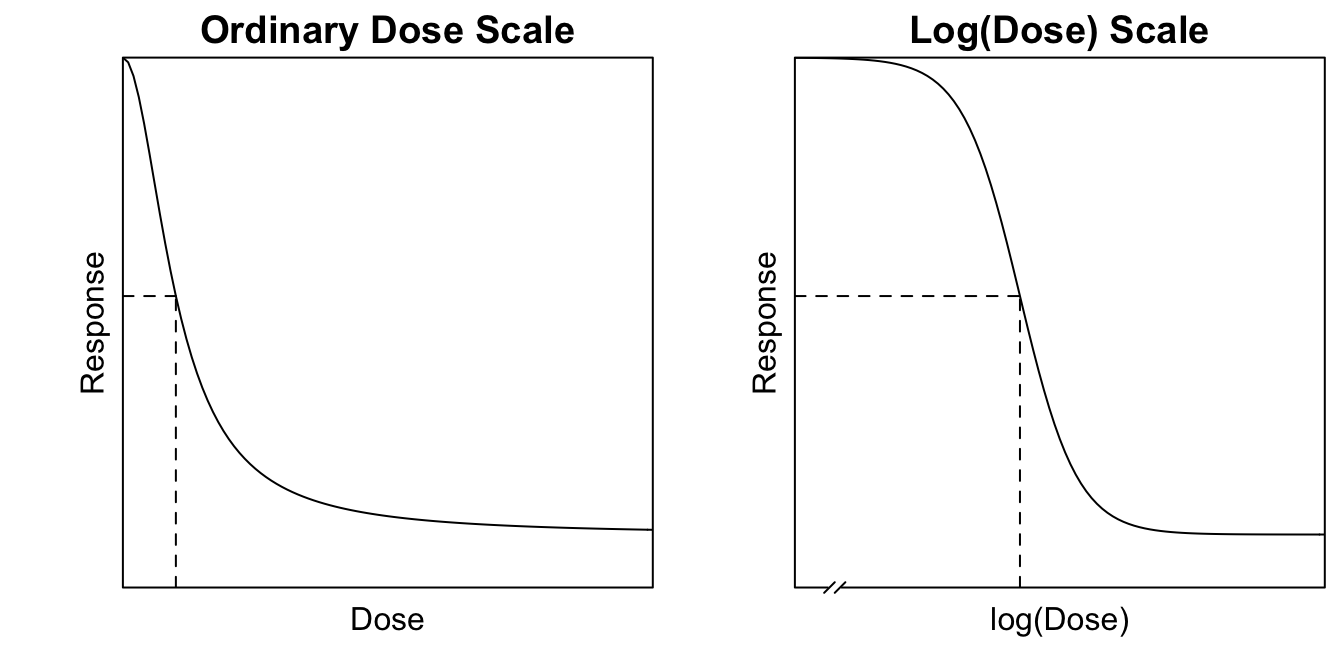
\includegraphics{Rstats4ag_files/figure-latex/figrawvslog-1.pdf}
\caption{\label{fig:figrawvslog}\emph{The log-logistic curve plotted on ordinary dose axis and log(Dose) axis. The broken lines indicate the \(ED_{50}\) on the x-axis and on the y-axis. The broken line on the log(Dose axis) indicates that a zero-dose does not exist on a logarithmic axis.}}
\end{figure}

The ordinary dose-scale looks almost as an exponential decay curve apart form the upper part where there is a small bend. However, one of the nice properties of the log-logistic curves is that it is symmetric on the log(dose) scale (Figure \ref{fig:figrawvslog}). The inflection point is the \(ED_{50}\) whatever the dose scale. The broken lines in Figure \ref{fig:figrawvslog} show the location of \(ED_{50}\), and in equation 1 it is a natural parameter of the model. If zero-dose is used as control we must break the x-axis to indicate that the logarithm to zero does not exist.

\hypertarget{assessment-of-selectivity}{%
\section{Assessment of Selectivity}\label{assessment-of-selectivity}}

If we want to compare the phytotoxicity of two or more herbicides on the same plant species or maybe the selectivity of a herbicide upon a crop and a weed species, then we must compare several dose-response curves simultaneously and quantify our findings in relative terms. We must define a standard herbicide and/or a standard species.



\begin{figure}
\centering
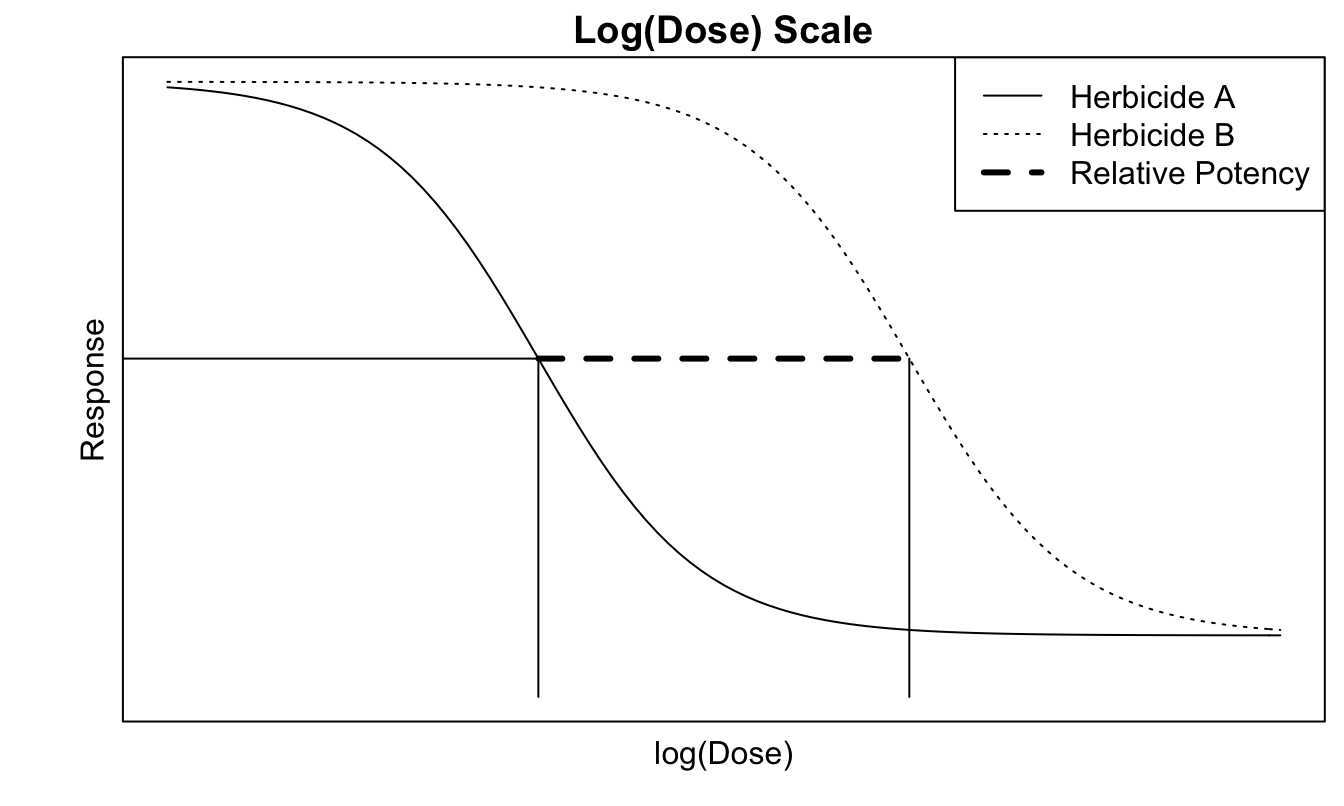
\includegraphics{Rstats4ag_files/figure-latex/figselect-1.pdf}
\caption{\label{fig:figselect}\emph{The relative potency at \(ED_{50}\) is the distance between the two curves. Note that the doses are on log scale and therefore the distance shown at the graph is the ratio between the two doses. In this instance the two curves are similar, i.e.~that they have the same upper and lower limit and slope. It is only the \(ED_{50}\) that differs.}}
\end{figure}

To make things simple we assume that we compare the action of two herbicides on the same plant species or at different plant species but with the same upper limit, \texttt{d}, and lower limit \texttt{c}.

The distance between the two dose-response curves at \(ED_{50}\) is a measure of the biological exchange rate between herbicides (Figure \ref{fig:figselect}), analogous to the more common practice of exchanging currencies, when traveling to foreign land. In toxicology and herbicide selectivity, we do not call it exchange rate, but the relative potency or relative strength, and when studying herbicide resistant biotypes of weeds, the resistance factor or R:S ratio.

For example, we know that to get adequate control of a common weed flora we need \(x_{B}\) g of a test herbicide and \(x_{A}\) g of the standard herbicide per unit area. Some will argue that \(ED_{50}\) is not at all of interest when it comes to controlling weeds, since we are never interested in only achieving 50\% control. While true from a practical standpoint, for the time being we will look at \(ED_{50}\) because it is a natural parameter of the log-logistic curve, and therefore it is an important parameter to classify toxic material. Later, we will look at the two additional ED-levels - \(ED_{10}\) to assess the crop tolerance and \(ED_{90}\) to assess the weed control. In general terms, we can define the relative potency as a response half way between the upper limit,\texttt{d}, and the lower limit \texttt{c}.

\[ R=\frac{x_{A}}{x_{B}} \]

Where the relative potency, \texttt{R}, can be defined at any \(ED_{x}\) level of which \(ED_{10}\), \(ED_{50}\), and \(ED_{90}\) are the most common levels in Weed Science. In ecotoxicology \(ED_{05}\) is common to define an no-effect level.

If the relative potency, R=1.0, then there is no difference between the effect of the two herbicides, i.e. \(x_{A}\) = \(x_{B}\), if \texttt{R\textless{}1} the herbicide dose of B is less effective than herbicide A and if \texttt{R\textgreater{}1} the herbicide A is more effective than herbicide B. So every time we calculate the relative potency, then we must know if the sheer ratio is different from 1.0.

In Figure \ref{fig:figselect}, the two dose response curves are similar in that the upper and lower limit are the same for the two curves as are the relative slopes, \texttt{b}. But what if the two curves are not similar (and this more commonly the rule rather than the exception in real life)?



\begin{figure}
\centering
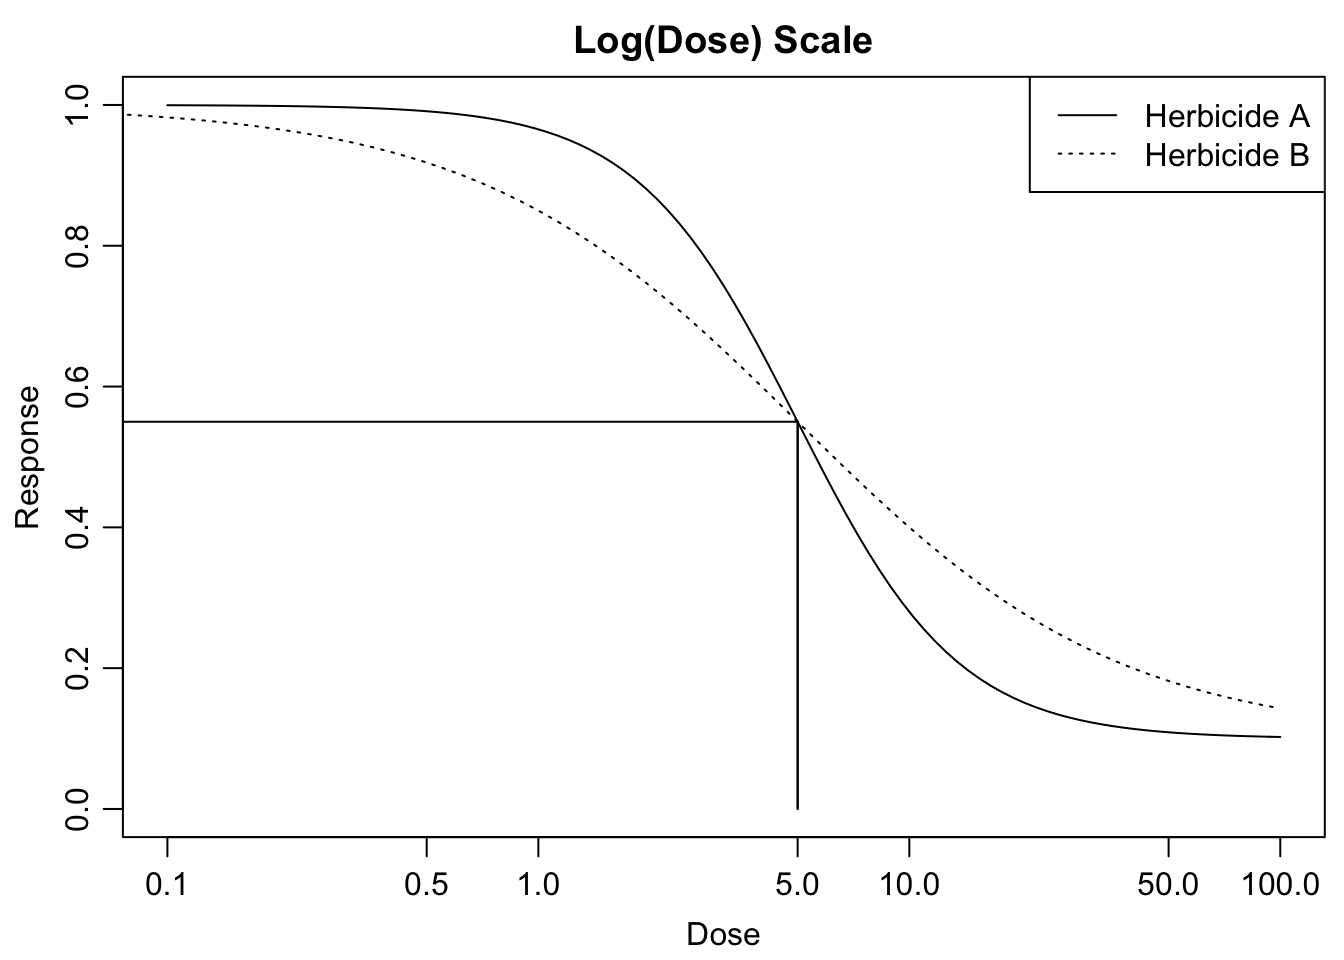
\includegraphics{Rstats4ag_files/figure-latex/figselect2-1.pdf}
\caption{\label{fig:figselect2}\emph{The two herbicides have similar upper and lower limit and \(ED_{50}\), but have different slopes.}}
\end{figure}

It is evident that in some cases \(ED_{50}\) does not give the right picture of toxicity when curves are not similar (Figure \ref{fig:figselect2}). Herbicide A is less potent above \(ED_{50}\) and more potent below \(ED_{50}\). Consider the example in Figure \ref{fig:figselect2} where the slopes are different but the \(ED_{50}\) s are identical. How should we report this? One way of doing it is to report the relative potency at relevant response levels. By defining Herbicide A as being the standard, it means that its \(ED_{x}\) is in the denominator. We get the following relative potencies:

\begin{verbatim}
## 
## Estimated effective doses
## 
##          Estimate Std. Error
## e:1:10 1.6667e+00 3.6316e-07
## e:1:50 5.0000e+00 5.1752e-07
## e:1:90 1.5000e+01 3.5880e-06
\end{verbatim}

\begin{verbatim}
## 
## Estimated effective doses
## 
##          Estimate Std. Error
## e:1:10 5.5556e-01 1.7824e-07
## e:1:50 5.0000e+00 1.2011e-06
## e:1:90 4.5000e+01 2.6206e-05
\end{verbatim}

\begin{verbatim}
##    e:1:10    e:1:50    e:1:90 
## 2.9999968 1.0000014 0.3333346
\end{verbatim}

\begin{itemize}
\tightlist
\item
  Herbicide A the doses are 1.67, 5, 15` for \(ED_{10}\), \(ED_{50}\) and \(ED_{90}\), respectively.
\item
  Herbicide B the doses are 0.56, 5, 45 for \(ED_{10}\), \(ED_{50}\) and \(ED_{90}\),respectively.
\item
  And the relative potencies are 3, 1, 0.33 at \(ED_{10}\), \(ED_{50}\) and \(ED_{90}\), respectively when Herbicide A is the standard.
\end{itemize}

Note how the relative potency changes from 3.0 at \(ED_{10}\) to 0.33 at \(ED_{90}\). Above \(ED_{50}\) herbicide B is more potent than herbicide A, but this changes below \(ED_{50}\) where the herbicide A now is most potent. This problem is looked at in more detailed in the \protect\hyperlink{doseresponse1}{previous chapter on dose response curves}.

The \(ED_{50}\) somewhat resembles the \(LD_{50}\) (or dose required to cause 50\% mortality in a test population) as an estimate in acute toxicity in toxicology, it does not tell the full story in Weed science. Particularly, when we wish to compare the selectivity of a herbicide on a crop and a weed flora, be it predominant weed species or not. \(ED_{50}\) contains much more information than do \(LD_{50}\), but becomes more difficult to interpret because we typically deal with continuous responses in Weed Science.



\begin{figure}
\centering
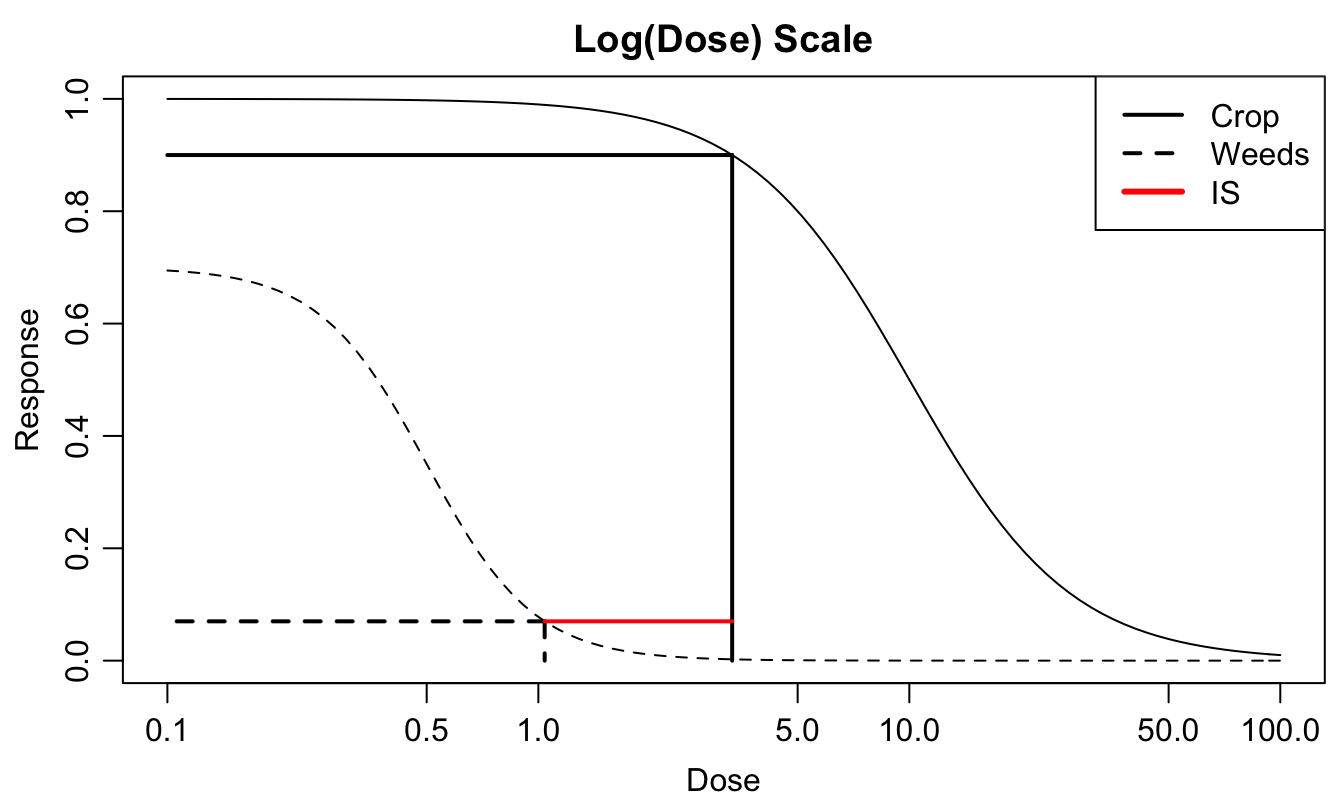
\includegraphics{Rstats4ag_files/figure-latex/figselect3-1.pdf}
\caption{\label{fig:figselect3}\emph{The assessment of the Selectivity Index for a crop and a weed or a group of weeds.}}
\end{figure}

\hypertarget{selectivity-index}{%
\section{Selectivity index}\label{selectivity-index}}

Since herbicides may have an effect on any plant, be it crop or weeds, we sometimes have to accept a small decrease in the yield of the crop growing in a weed free environment. For example a 10\% decrease might be tolerated, \(ED_{10}\), while a 90\% control of the weed, \(ED_{90}\), is considered a reasonable control level of the weeds. The \(ED_{10}\) for the crop is 3.33 and the \(ED_{90}\) for the weed is 1.04. Consequently the Selectivity Index is 3.20. As seen in Figure \ref{fig:figselect3}, the upper limits for the crop and the weed are different.

In the development of herbicides the companies screen virtually 10,000's of compounds, only a small fraction of which may have some activity. In order to handle this immense amount of information, they must unambiguously define the selectivity of herbicides in the development phase. By accepting a 10\% yield loss of the crop growing in weed free environment and by being satisfied with a 90\% effect on the weeds growing in crop free environment, we get an Index of Selectivity, IS:

\[   IS=\frac{{[ED_{10}]_{crop}}}{{[ED_{90}]_{weeds}}} \]

However, the same situation arises when we compare herbicide resistant biotypes with susceptible biotypes. Obviously, if there is target site resistance and a yield penalty we expect difference in response in untreated control. If it is metabolic resistance where no yield penalty has been observed, we can still have different untreated control response. This fact of differences in upper limit among curves are not being solved by making the untreated control equal to 100 and adjust the responses within biotypes accordingly. This often-ignored problem is dealt with in the \protect\hyperlink{doseresponse1}{previous chapter on dose-response curves}.

\hypertarget{vertical-and-horizontal-assessment}{%
\section{Vertical and Horizontal Assessment}\label{vertical-and-horizontal-assessment}}

Vertical and horizontal assessment of herbicide effect is shown graphically in Figure \ref{fig:figvh}.

\hypertarget{vertical-assessment}{%
\subsection{Vertical assessment}\label{vertical-assessment}}

Vertical assessment compares plant response at some preset dose levels. This is the most common method for evaluating herbicides in the field. If doses were chosen close to the upper or lower limit of the curves, differences between treatments would be less than if they were chosen in the middle part of the curve. If we are only working at dose-ranges in the middle part of the curves then, in this particular instance, differences would be almost independent of dose-levels. Consequently, the middle region is obviously the optimal part of the curve to obtain information about differences of effects in this particular graph where the curves are looking very similar. This, however, does not apply when the curves have different slopes as shown in Figure \ref{fig:figselect3}.

The curves show that if a herbicide is tested with or without an adjuvant in a factorial experiment, we may get significant interactions, because the differences of effects are not constant. As this interaction is dose dependent due to the S-shaped curves, it may be considered trivial and of little biological significance, when we appraise the selective action of the herbicide. If we choose only dose-ranges in the middle part of the curves, then differences are constant and independent of dose-levels and the interaction would disappear, i.e.~the effects are additive.

\hypertarget{horizontal-assessment}{%
\subsection{Horizontal assessment}\label{horizontal-assessment}}

Horizontal assessment is the method we used in the herbicide selectivity section and it answers the question many farmers are interested in: which dose should I use of herbicide A to get the same effect as with herbicide B (the biological exchange rate of two herbicide products). Usually, herbicides are tested in two to three doses and their efficacy is compared with either the untreated control or with some standard herbicide treatment. Rarely, we have so many doses in the field that we actually are able to fit the entire dose response curve.



\begin{figure}
\centering
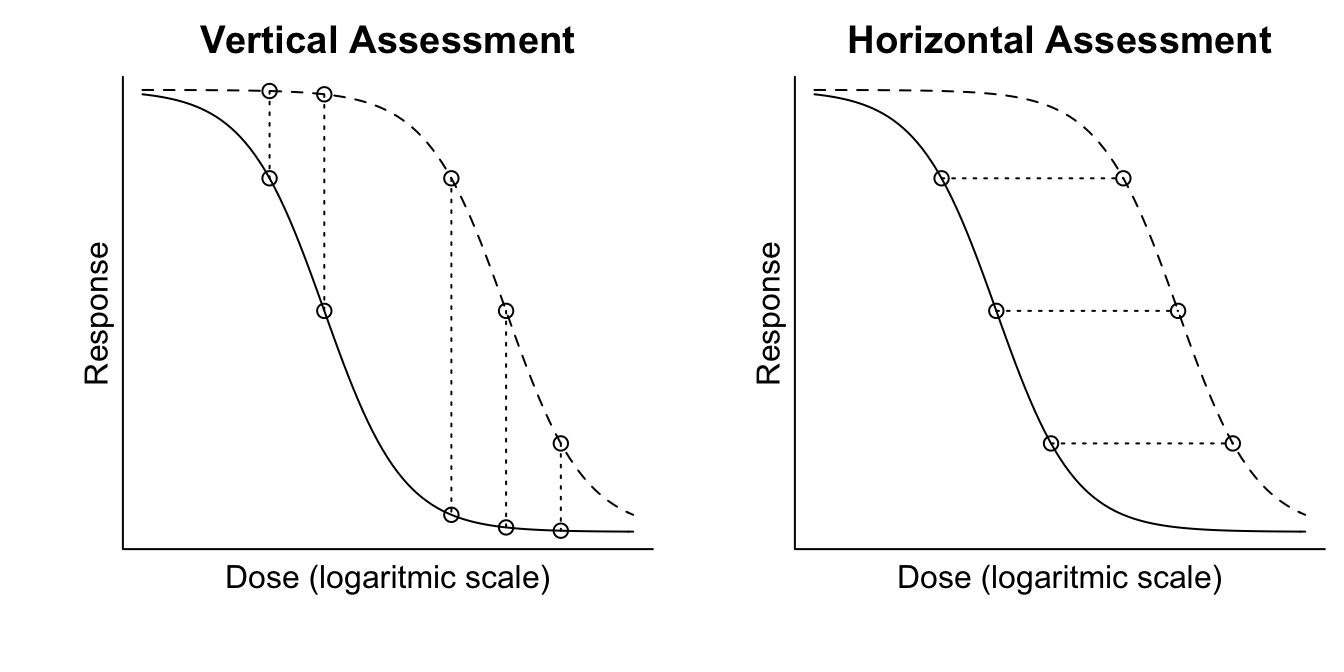
\includegraphics{Rstats4ag_files/figure-latex/figvh-1.pdf}
\caption{\label{fig:figvh}\emph{Vertical and horizontal comparison of efficacy of say two herbicide on the same plant species.}}
\end{figure}

Even though the horizontal assessment above seems straight forward, it is not always the case. With continuous response variables comparing dose-response curves with different upper and lower limits is not just a trivial task to compare curves. The differences in upper and lower limits of different dose-response curves are sometimes important as they tell a story about the experiments. In the \protect\hyperlink{doseresponse1}{Dose-Response Curve chapter} we briefly discuss it. The bottom line here is that comparison is not a matter of statistics, but a matter of biology, and thus rather complicated.

\begin{center}\rule{0.5\linewidth}{0.5pt}\end{center}

\hypertarget{plant-competition-experiments}{%
\chapter{Plant Competition Experiments}\label{plant-competition-experiments}}

Competition experiments are a staple of weed science. Typically, we often want to assess the effect of weed density or duration of competition on crop yield. There is an ongoing debate about the appropriateness of using density and not for example plant cover. We will not go into this debate, but stick to density of plant, because the methods of analyzing data remain the same whether the independent variable, \texttt{x}, is density or plant cover.

One of the important questions is,how do we assess competition and when does it start. In principle competition starts at germination and is a question of the resources:

\begin{itemize}
\tightlist
\item
  Light
\item
  Nutrients
\item
  Water
\item
  ``Space''
\end{itemize}

The three first factors are rather easy to quantify, but the fourth one is more intangible it is dependent on the growth habits of the weeds, e.g.~prostrate, erect and the ability of the crop to outgrow the weeds. Whatever the reason for competition, it often boils down to the relationship in Figure \ref{fig:figcompshape}; when will the relationship divert from a straight line.

\hypertarget{yield-density-and-yield-loss}{%
\section{Yield, Density and Yield Loss}\label{yield-density-and-yield-loss}}

The general plant competition and crop yield loss relationships are consider the same, a rectangular hyperbola. In Figure \ref{fig:figcompshape} we have a classical intra-specific competition relationship (A), and a yield loss relationship (B). Competition materializes when the curve diverts from the straight line. The initial straight line means that putting a new plant into the system just increases the yield the same way as all the other individuals contribute initially. When individual plants begin compete with each other for resources, because of high density, then the curves diverts from the straight line.

In Figure \ref{fig:figcompshape}B, the percentage yield loss is based upon the yield without the presence of weeds. The competition (inter-specific competition) for resources materializes itself immediately. When the line diverts from the straight line relationship there will also be some intra-specific competition among the weeds. If there is no competition between crop and weeds at all, then the slope of the curve in Figure \ref{fig:figcompshape}B would be zero, or no change in yield whatever the density of weeds.



\begin{figure}
\centering
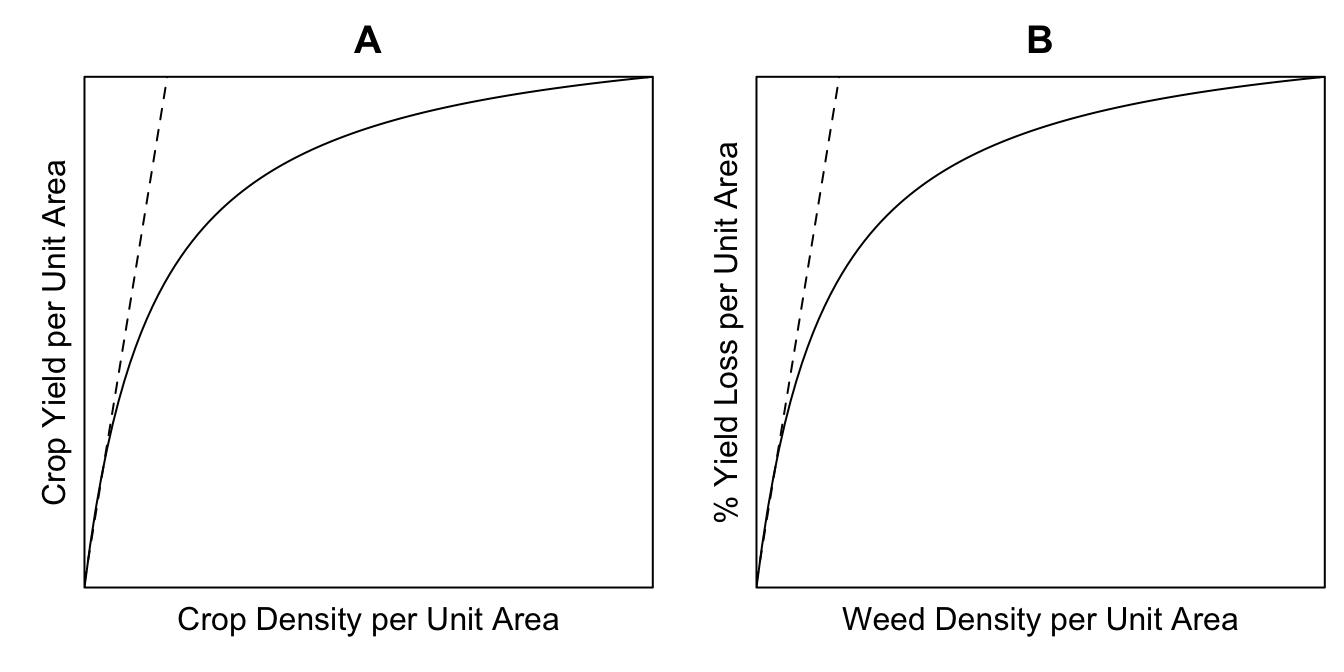
\includegraphics{Rstats4ag_files/figure-latex/figcompshape-1.pdf}
\caption{\label{fig:figcompshape}\emph{Competition within the same species, often denoted intra-specific competition (A). Yield loss function based on the percentage yield loss relative to the yield in weed free environment (B).}}
\end{figure}

If the yield is a crop and the density is weeds per unit area then the the competition (inter-specific competition) materializes in exactly the same way. But now the competition begins from the very start. If there is no competition between crop and weed then the slope of the curve would be zero, viz no change in yield whatever the density of weeds.

The first example is a study conducted near Lingle, Wyoming over two years. In this study, volunteer corn densities ranging from 0 to 2.4 plants/\(m^2\) were planted along with dry edible beans to document the bean yield loss from increasing volunteer corn density.

\begin{Shaded}
\begin{Highlighting}[]
\KeywordTok{read.csv}\NormalTok{(}\StringTok{"http://rstats4ag.org/data/volcorn.csv"}\NormalTok{)->VolCorn}
\NormalTok{VolCorn}\OperatorTok{$}\NormalTok{yr<-}\KeywordTok{as.factor}\NormalTok{(VolCorn}\OperatorTok{$}\NormalTok{yr)}
\NormalTok{VolCorn}\OperatorTok{$}\NormalTok{reps<-}\KeywordTok{as.factor}\NormalTok{(VolCorn}\OperatorTok{$}\NormalTok{reps)}

\KeywordTok{head}\NormalTok{(VolCorn,}\DataTypeTok{n=}\DecValTok{3}\NormalTok{)}
\end{Highlighting}
\end{Shaded}

\begin{verbatim}
##     yr reps dens    y.pct y.kg
## 1 2009    1    0 3.283996 6273
## 2 2009    2    0 9.466543 5872
## 3 2009    3    0 4.625347 6186
\end{verbatim}

The variable `yr' is the year the study was completed (either 2008 or 2009), \texttt{reps} denotes the replicate (1 through 4), `dens' is the volunteer corn density in plants/\(m^2\) (0 to 2.4), `y.pct' is the percentage dry bean yield loss as compared with the zero volunteer corn density, and `y.kg' is the dry bean yield in kg/ha.

\href{http://onlinelibrary.wiley.com/doi/10.1111/j.1744-7348.1985.tb01567.x/pdf}{Cousens 1985} proposed a re-parameterization of a rectangular hyperbola (perhaps better known as Michaelis-Menten) model as a tool to analyze competition experiments, and the \texttt{drc} is well suited for this type of analysis \href{http://www.jstatsoft.org/v12/i05/paper}{Ritz and Streibig 2005}. This package must be loaded with the code:

\begin{Shaded}
\begin{Highlighting}[]
\KeywordTok{library}\NormalTok{(drc)}
\end{Highlighting}
\end{Shaded}

The \texttt{drm()} function can be used to fit a variety of non-linear models, including the Michaelis-Menten model. The code to fit the Michaelis-Menten model to the volunteer corn data is for one of the two years, 2009, by using the argument \texttt{data=VolCorn,\ subset=yr==2009,}

\begin{Shaded}
\begin{Highlighting}[]
\KeywordTok{drm}\NormalTok{(y.pct }\OperatorTok{~}\StringTok{ }\NormalTok{dens, }\DataTypeTok{fct=}\KeywordTok{MM.2}\NormalTok{(}\DataTypeTok{names=}\KeywordTok{c}\NormalTok{(}\StringTok{"Vmax"}\NormalTok{,}\StringTok{"K"}\NormalTok{)), }\DataTypeTok{data=}\NormalTok{VolCorn, }
    \DataTypeTok{subset=}\NormalTok{yr}\OperatorTok{==}\DecValTok{2009}\NormalTok{, }\DataTypeTok{na.action=}\NormalTok{na.omit)->y2009.MM2}
\KeywordTok{summary}\NormalTok{(y2009.MM2)}
\end{Highlighting}
\end{Shaded}

\begin{verbatim}
## 
## Model fitted: Michaelis-Menten (2 parms)
## 
## Parameter estimates:
## 
##                  Estimate Std. Error t-value p-value
## Vmax:(Intercept)  66.7415    73.8753  0.9034  0.3782
## K:(Intercept)      2.6490     4.8209  0.5495  0.5894
## 
## Residual standard error:
## 
##  13.32239 (18 degrees of freedom)
\end{verbatim}

Obviously, the \texttt{Vmax} and \texttt{K} parameter of the Michaelis-Menten model were non-significant, the reason is that the range of density of weeds were not large enough, we only catch the linear part (Figure \ref{fig:figvolcornextrapolate}).



\begin{Shaded}
\begin{Highlighting}[]
\KeywordTok{par}\NormalTok{(}\DataTypeTok{mfrow =} \KeywordTok{c}\NormalTok{(}\DecValTok{1}\NormalTok{, }\DecValTok{1}\NormalTok{), }\DataTypeTok{mar=}\KeywordTok{c}\NormalTok{(}\FloatTok{3.2}\NormalTok{,}\FloatTok{3.2}\NormalTok{,.}\DecValTok{5}\NormalTok{,.}\DecValTok{5}\NormalTok{), }\DataTypeTok{mgp=}\KeywordTok{c}\NormalTok{(}\DecValTok{2}\NormalTok{,.}\DecValTok{7}\NormalTok{,}\DecValTok{0}\NormalTok{))}
\KeywordTok{plot}\NormalTok{(y2009.MM2,}\DataTypeTok{log=}\StringTok{""}\NormalTok{, }
     \DataTypeTok{ylab=} \StringTok{"Percent Sugarbeet Yield Loss"}\NormalTok{,}
     \DataTypeTok{xlab=}\StringTok{"Volunteer Corn Density"}\NormalTok{,}
     \DataTypeTok{ylim=}\KeywordTok{c}\NormalTok{(}\DecValTok{0}\NormalTok{,}\DecValTok{70}\NormalTok{), }\DataTypeTok{xlim=}\KeywordTok{c}\NormalTok{(}\DecValTok{0}\NormalTok{,}\DecValTok{10}\NormalTok{), }\DataTypeTok{bty=}\StringTok{"l"}\NormalTok{)}
\KeywordTok{abline}\NormalTok{(}\DataTypeTok{h=}\FloatTok{66.7}\NormalTok{, }\DataTypeTok{lty=}\DecValTok{2}\NormalTok{)}
\end{Highlighting}
\end{Shaded}

\begin{figure}
\centering
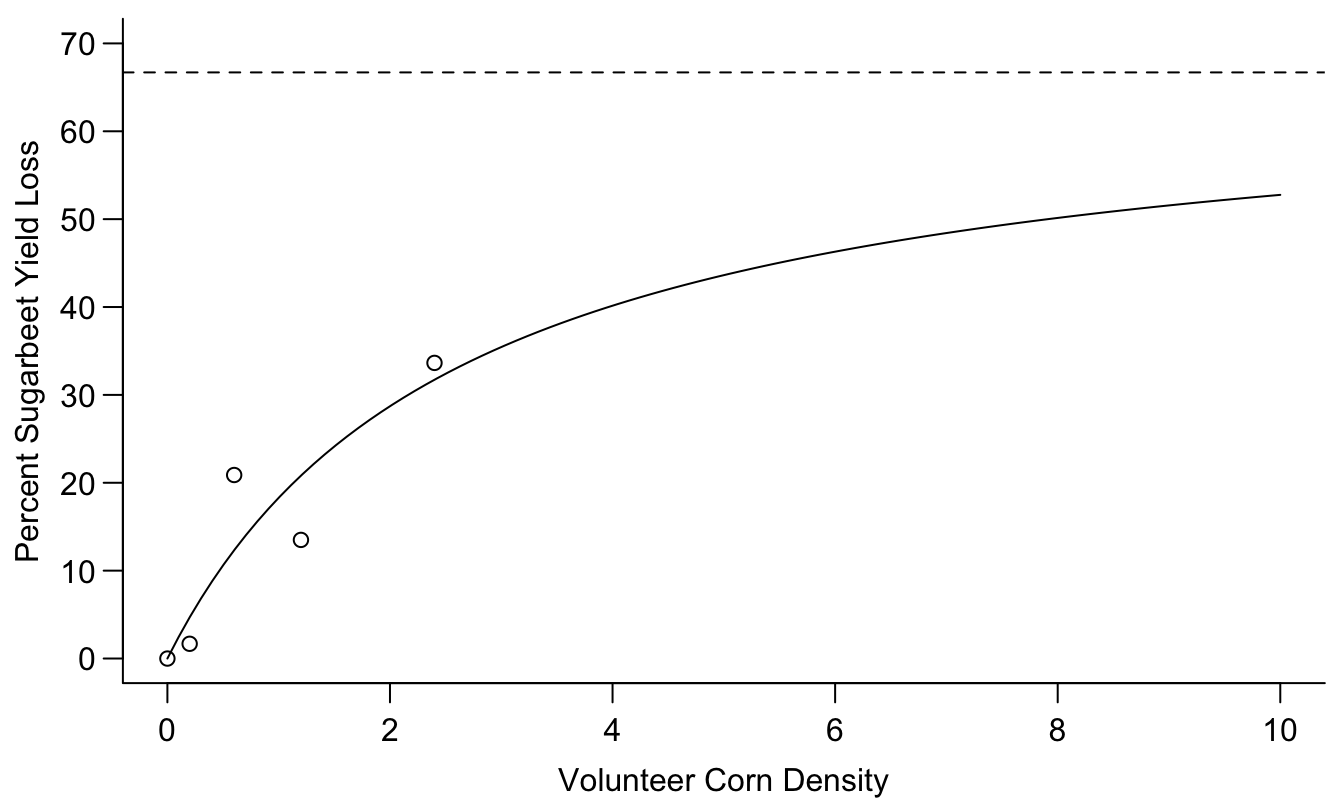
\includegraphics{Rstats4ag_files/figure-latex/figvolcornextrapolate-1.pdf}
\caption{\label{fig:figvolcornextrapolate}\emph{Yield loss curve with a two parameter Michaelis-Menten's curve (the argument in \texttt{drm()} is \texttt{fct=MM.2()}. The \texttt{Vmax} is the upper limit, shown with the broken horizontal line, and \texttt{k} is the rate constant.}}
\end{figure}

All functions in the \texttt{drc} package are defined in the \texttt{getMeanFunctions()} by writing \texttt{?MM.3} or \texttt{?MM.2} you can see the help on the curve fitting function.

\[y=c + \frac{d-c}{1+(e/x)} .\]

The suffix 3 or 2 defines how many asymptotes we use. The most common one is \texttt{MM.2} where there is only one upper limit \emph{d}, in this context often referred to as \emph{Vmax}. If you compare the model above with the log-logistic models, used in the selectivity and dose-response chapter, they look almost identical except that \emph{b} in the log-logistic does not exist in \texttt{MM.2} or \texttt{MM.3}, because for this case \emph{b}=1. The standard error of the parameter estimates reveals that none of the two parameters are significantly different from zero. This is due to the fact that only the first part of the curve is supported by experimental data as seen in Figure \ref{fig:figvolcornextrapolate}; there is no data to support the upper limit of the curve.

The tradition in weed science, as mentioned above, is to reparametrizise the Michaelis-Menten model and use:

\[Y_L = \frac{Ix}{1+Ix/A} .\]

which was proposed by Cousens (1985), where \texttt{A} now is the upper limit and \texttt{I} is the initial slope of the curve as shown Figure \ref{fig:figcompshape}. This reparametrization is available in the `drc' package by using the `yieldLoss()' function as shown below:

\begin{Shaded}
\begin{Highlighting}[]
\KeywordTok{yieldLoss}\NormalTok{(y2009.MM2, }\DataTypeTok{interval=}\StringTok{"as"}\NormalTok{)}
\end{Highlighting}
\end{Shaded}

\begin{verbatim}
## 
## Estimated A parameters
## 
##   Estimate Std. Error   Lower   Upper
## 1   66.741     73.875 -88.465 221.948
## 
## 
## Estimated I parameters
## 
##   Estimate Std. Error   Lower   Upper
## 1   25.195     18.749 -14.196  64.585
\end{verbatim}

The upper limit, which is called \texttt{Vmax} in the Michaelis-Menten and \texttt{A} in the yieldLoss function is the same 67\% and the rate constant in the Michaelis-Menten is 2.64 (corresponding to ED50 in the Log-logistic), but for the Cousens rectangular hyperbola the initial slope is 25. Of course the parameters of the \texttt{yieldLoss()} function were not different from zero either.

Looking at the yield loss curve one could suspect that a straight line relationship applies. We test the regression against the most general model an ANOVA:

\begin{Shaded}
\begin{Highlighting}[]
\NormalTok{lm.Y2009<-}\KeywordTok{lm}\NormalTok{(y.pct }\OperatorTok{~}\StringTok{ }\NormalTok{dens,}\DataTypeTok{data=}\NormalTok{VolCorn, }\DataTypeTok{subset=}\NormalTok{yr}\OperatorTok{==}\DecValTok{2009}\NormalTok{)}
\NormalTok{ANOVA.Y2009<-}\KeywordTok{lm}\NormalTok{(y.pct }\OperatorTok{~}\StringTok{ }\KeywordTok{factor}\NormalTok{(dens), }\DataTypeTok{data=}\NormalTok{VolCorn, }\DataTypeTok{subset=}\NormalTok{yr}\OperatorTok{==}\DecValTok{2009}\NormalTok{)}
\KeywordTok{anova}\NormalTok{(lm.Y2009,ANOVA.Y2009)}
\end{Highlighting}
\end{Shaded}

\begin{verbatim}
## Analysis of Variance Table
## 
## Model 1: y.pct ~ dens
## Model 2: y.pct ~ factor(dens)
##   Res.Df    RSS Df Sum of Sq      F Pr(>F)
## 1     18 3241.9                           
## 2     15 2637.2  3    604.71 1.1465 0.3625
\end{verbatim}

The test for lack of fit is non-significant (p=0.36) so we can confidently assume the straight line gives a good description of the relationship.

\begin{Shaded}
\begin{Highlighting}[]
\KeywordTok{summary}\NormalTok{(lm.Y2009)}
\end{Highlighting}
\end{Shaded}

\begin{verbatim}
## 
## Call:
## lm(formula = y.pct ~ dens, data = VolCorn, subset = yr == 2009)
## 
## Residuals:
##     Min      1Q  Median      3Q     Max 
## -30.013  -6.501   1.457   7.370  27.645 
## 
## Coefficients:
##             Estimate Std. Error t value Pr(>|t|)   
## (Intercept)    2.498      4.285   0.583  0.56717   
## dens          13.002      3.475   3.741  0.00149 **
## ---
## Signif. codes:  0 '***' 0.001 '**' 0.01 '*' 0.05 '.' 0.1 ' ' 1
## 
## Residual standard error: 13.42 on 18 degrees of freedom
## Multiple R-squared:  0.4374, Adjusted R-squared:  0.4062 
## F-statistic:    14 on 1 and 18 DF,  p-value: 0.001495
\end{verbatim}

Sugarbeet yield loss increases by 13\% with each volunteer corn plant/m\(^2\) that is added into the system.



\begin{Shaded}
\begin{Highlighting}[]
\KeywordTok{library}\NormalTok{(dplyr)}
\NormalTok{Yield.m<-}\KeywordTok{subset}\NormalTok{(VolCorn,yr}\OperatorTok{==}\DecValTok{2009}\NormalTok{) }\OperatorTok
\StringTok{  }\KeywordTok{group_by}\NormalTok{(dens) }\OperatorTok
\StringTok{  }\KeywordTok{summarise}\NormalTok{(}\DataTypeTok{Yieldloss=}\KeywordTok{mean}\NormalTok{(y.pct))}

\KeywordTok{par}\NormalTok{(}\DataTypeTok{mfrow =} \KeywordTok{c}\NormalTok{(}\DecValTok{1}\NormalTok{, }\DecValTok{1}\NormalTok{), }\DataTypeTok{mar=}\KeywordTok{c}\NormalTok{(}\FloatTok{3.2}\NormalTok{,}\FloatTok{3.2}\NormalTok{,.}\DecValTok{5}\NormalTok{,.}\DecValTok{5}\NormalTok{), }\DataTypeTok{mgp=}\KeywordTok{c}\NormalTok{(}\DecValTok{2}\NormalTok{,.}\DecValTok{7}\NormalTok{,}\DecValTok{0}\NormalTok{))}
\KeywordTok{plot}\NormalTok{(Yieldloss }\OperatorTok{~}\StringTok{ }\NormalTok{dens,}\DataTypeTok{data=}\NormalTok{Yield.m, }
     \DataTypeTok{ylab=}\StringTok{"Percent Sugarbeet Yield Loss"}\NormalTok{, }
     \DataTypeTok{xlab=}\StringTok{"Volunteer corn density"}\NormalTok{, }\DataTypeTok{bty=}\StringTok{"l"}\NormalTok{)}
\KeywordTok{abline}\NormalTok{(lm.Y2009)}
\KeywordTok{plot}\NormalTok{(y2009.MM2,}\DataTypeTok{log=}\StringTok{""}\NormalTok{, }\DataTypeTok{add=}\NormalTok{T, }\DataTypeTok{lty=}\DecValTok{2}\NormalTok{)}
\end{Highlighting}
\end{Shaded}

\begin{figure}
\centering
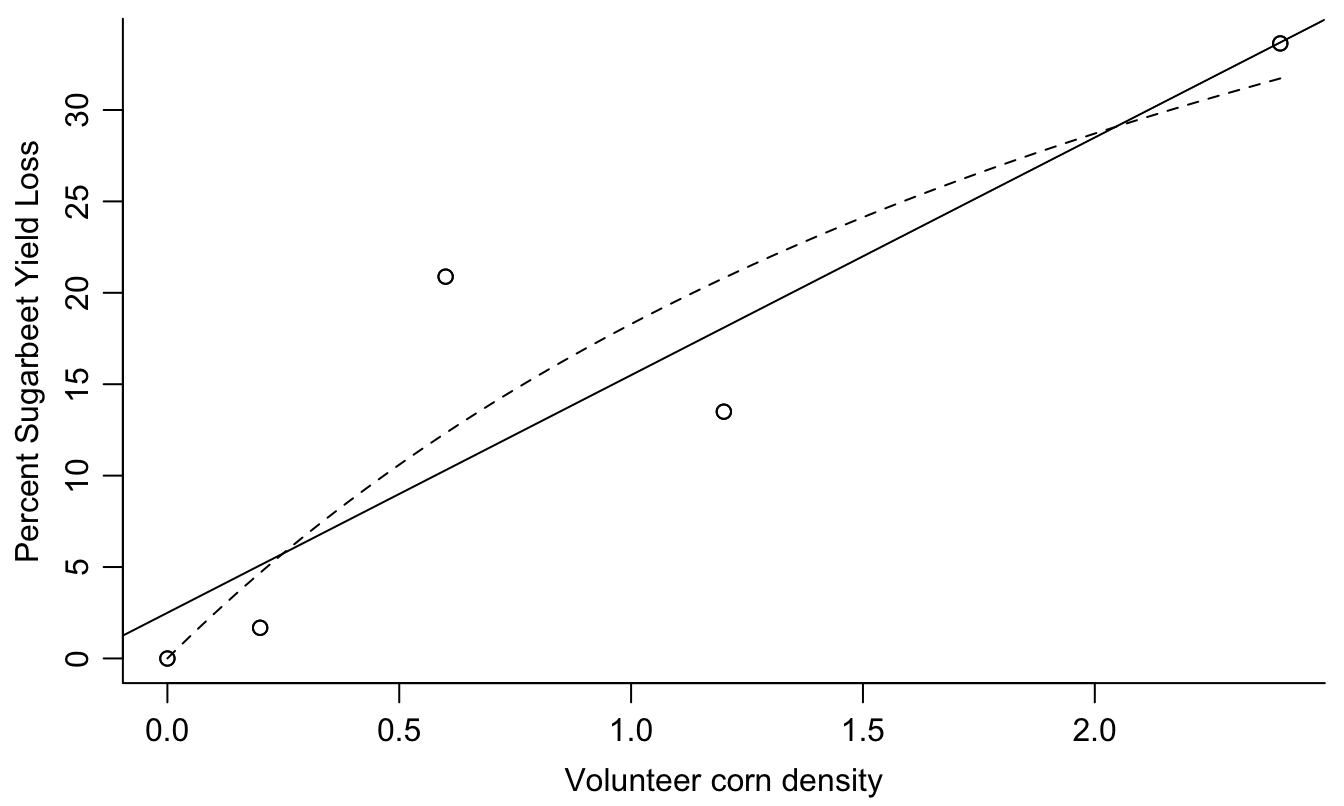
\includegraphics{Rstats4ag_files/figure-latex/figvolcornmodelcomp-1.pdf}
\caption{\label{fig:figvolcornmodelcomp}\emph{The linear model fit with a slope of 13 meaning that for every unit density of corn we get a yield decrease of 13\%. The broken line is the nonlinear fit from shown in Figure \ref{fig:figvolcornextrapolate}.}}
\end{figure}

The assumption of a straight line relationship in Figure \ref{fig:figvolcornmodelcomp} is justified by the test for lack of fit and we can conclude we loose 13\% yield per each volunteer corn plant. However, it is important to recognize that the further we extrapolate beyond the volunteer corn densities used in the study, the more likely the linear fit is to provide nonsensical yield loss estimates.

One issue with expressing yield loss as a function of the weed-free is it relies heavily on the weed-free control treatments from a particular study. When regression is used, it is possible to use the density relationship (in addition to the weed-free control treatment) to provide a more robust estimate of crop yield in the absence of weed competition. The weed-free yield can be estimated by using the following re-parameterization of the rectangular hyperbolic model (also proposed by Cousens 1985):

\[Yield = Y_0(1-(\frac{Ix}{100(1+Ix/A)})) \]

where \emph{Y\textsubscript{0}} is the intercept with the yield axis when weed density is zero. Of course it requires that the curve is well described over the range of relevant weed densities \href{http://www.wssajournals.org/doi/pdf/10.1614/WS-D-13-00159.1}{Ritz, Kniss and Streibig 2015}.

\hypertarget{replacement-series}{%
\section{Replacement Series}\label{replacement-series}}

The replacement series can assess interference, niche differentiation, resource utilization, and productivity in simple mixtures of two species. Of course more than two species can be used as long as the total density remains the same, but the interpretation of results becomes very difficult. The species are growing at the same total density, but the proportion between the two species vary. One of the good things about replacement series is that if the replacement graphs looks like the one in Figure 5, it could be the reference, because with linear relationships in Figure 5 shows no competition; the two species do not interfere with each others growth. As discuss earlier, when there is a straight line relationship between yield and density of a species ( Figure 1), the second species does not interfere. If there is a curved relationship there is intraspecific and/or inter specific competition. The intraspecific competition can only be assessed if a species is grown in pure stand.

The density dependence, maximum density determined by experimenter, impedes generalization for a replacement series. And as always, we only get a snapshot of what is going on in an otherwise dynamic competition scenario. In order to avoid criticisms, however, researchers should appreciate the assumptions and limitations of this methodology \href{http://onlinelibrary.wiley.com/doi/10.1046/j.1365-2745.2000.00470.x/pdf}{Jollife 2000}



\begin{figure}
\centering
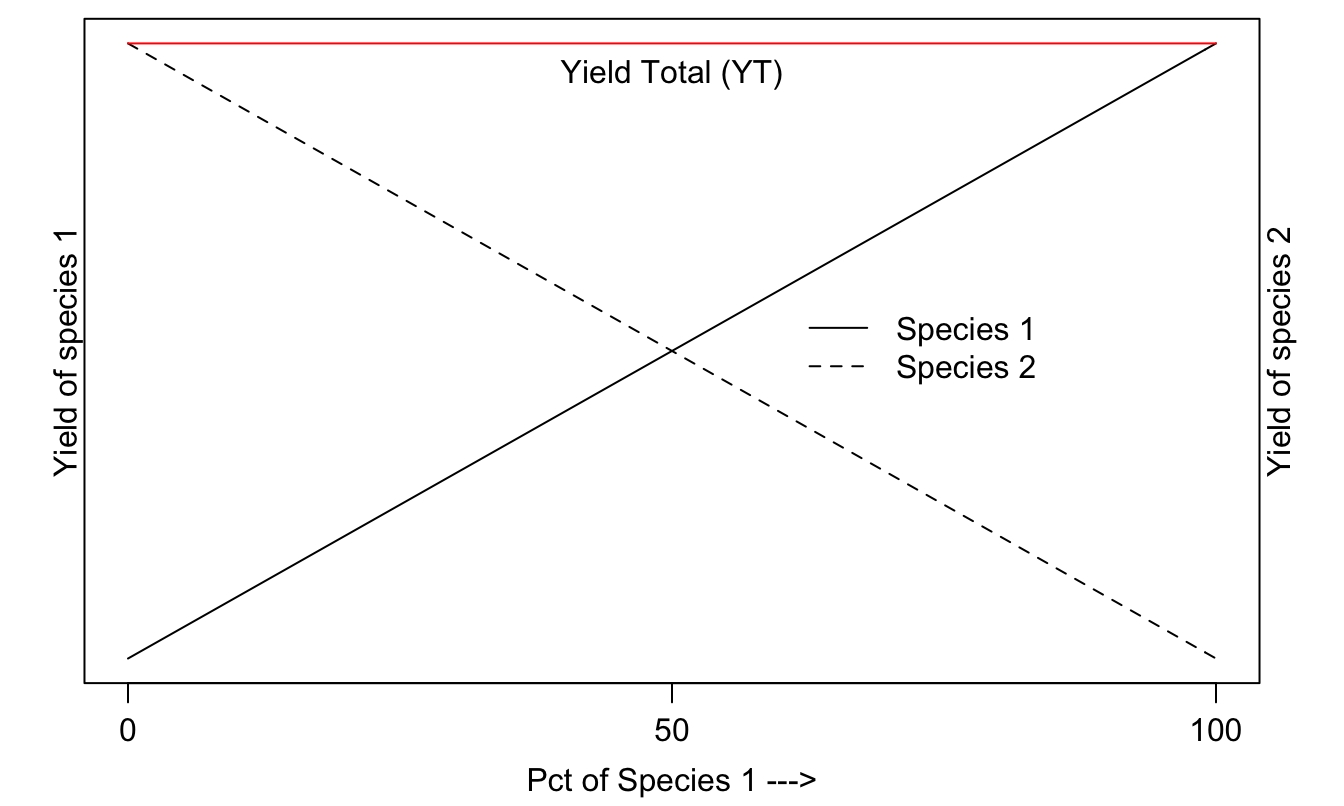
\includegraphics{Rstats4ag_files/figure-latex/figrepser-1.pdf}
\caption{\label{fig:figrepser}\emph{The frame of reference for replacement series with two species where there is no competition between species and the Yield Total (YT) does not change which ever the combination of the two species is. The two species do not need to have the same maximum yield in monoculture.}}
\end{figure}

The philosophy of the replacement series is that the carrying capacity, in terms of say biomass, on a unit of land is constant whatever the proportion of the species.

The example uses a barley crop grown together with the weed Amsinckia menziesii. The experiment was run in greenhouse with the intention of having 20 plants in total in pots of 20 cm in diameter. After 20 days the plants were harvested and the actual number of plants were counted and the biomass per species measured.

The dataset \texttt{Replacement\ series.csv} is a mixture of \texttt{csv} and \texttt{csv2} files, because the students who did the experiments came form continental Europe or Australia. It means the continental Europeans use the semicolon as variable separator mixed with the Australian's decimal separator of dot. This mess is taken care of by using the \texttt{read.table()} function.

As we have to use the percent of either species as independent variable to fit regression models we have to define new variables \texttt{Pct.Amsinckia} and \texttt{Pct.Barley}.

\begin{Shaded}
\begin{Highlighting}[]
\NormalTok{Replace}\FloatTok{.1}\NormalTok{<-}\KeywordTok{read.table}\NormalTok{(}\StringTok{"http://rstats4ag.org/data/ReplacementSeries.csv"}\NormalTok{,}
                      \DataTypeTok{header=}\OtherTok{TRUE}\NormalTok{, }\DataTypeTok{sep=}\StringTok{";"}\NormalTok{, }\DataTypeTok{dec=}\StringTok{"."}\NormalTok{)}
\NormalTok{Replace}\FloatTok{.1}\OperatorTok{$}\NormalTok{Pct.Amsinckia<-}\KeywordTok{with}\NormalTok{(Replace}\FloatTok{.1}\NormalTok{,D.Amsinckia}\OperatorTok{*}\DecValTok{100}\OperatorTok{/}\NormalTok{(D.Amsinckia}\OperatorTok{+}\NormalTok{D.Barley))}
\NormalTok{Replace}\FloatTok{.1}\OperatorTok{$}\NormalTok{Pct.Barley<-}\StringTok{   }\KeywordTok{with}\NormalTok{(Replace}\FloatTok{.1}\NormalTok{,D.Barley}\OperatorTok{*}\DecValTok{100}\OperatorTok{/}\NormalTok{(D.Amsinckia}\OperatorTok{+}\NormalTok{D.Barley))}
\KeywordTok{head}\NormalTok{(Replace}\FloatTok{.1}\NormalTok{,}\DataTypeTok{n=}\DecValTok{3}\NormalTok{)}
\end{Highlighting}
\end{Shaded}

\begin{verbatim}
##   D.Amsinckia D.Barley Harvest.time B.Amsinckia B.Barley Pct.Amsinckia Pct.Barley
## 1           0       14   14.05.2014           0     98.1             0        100
## 2           0       32   14.05.2014           0    112.7             0        100
## 3           0       21   14.05.2014           0     94.5             0        100
\end{verbatim}

First we try straight line relationships and illustrate the fit and with an analysis of residuals.



\begin{Shaded}
\begin{Highlighting}[]
\NormalTok{lm.Amsinckia<-}\KeywordTok{lm}\NormalTok{(B.Amsinckia }\OperatorTok{~}\NormalTok{Pct.Amsinckia,}\DataTypeTok{data=}\NormalTok{Replace}\FloatTok{.1}\NormalTok{)}
\NormalTok{lm.Barley<-}\KeywordTok{lm}\NormalTok{(B.Barley }\OperatorTok{~}\NormalTok{Pct.Barley,}\DataTypeTok{data=}\NormalTok{Replace}\FloatTok{.1}\NormalTok{)}

\KeywordTok{par}\NormalTok{(}\DataTypeTok{mfrow =} \KeywordTok{c}\NormalTok{(}\DecValTok{2}\NormalTok{, }\DecValTok{2}\NormalTok{), }\DataTypeTok{mar=}\KeywordTok{c}\NormalTok{(}\FloatTok{3.2}\NormalTok{,}\FloatTok{3.2}\NormalTok{,.}\DecValTok{5}\NormalTok{,.}\DecValTok{5}\NormalTok{), }\DataTypeTok{mgp=}\KeywordTok{c}\NormalTok{(}\DecValTok{2}\NormalTok{,.}\DecValTok{7}\NormalTok{,.}\DecValTok{0}\NormalTok{))}
\KeywordTok{plot}\NormalTok{(B.Amsinckia }\OperatorTok{~}\NormalTok{Pct.Amsinckia,}\DataTypeTok{data=}\NormalTok{Replace}\FloatTok{.1}\NormalTok{, }\DataTypeTok{ylab=}\StringTok{"Yield of Amsinckia"}\NormalTok{,}
     \DataTypeTok{xlab=}\StringTok{"Percent of Amsinckia"}\NormalTok{)}
  \KeywordTok{legend}\NormalTok{(}\StringTok{"topleft"}\NormalTok{, }\StringTok{"A"}\NormalTok{, }\DataTypeTok{bty=}\StringTok{"n"}\NormalTok{)}
\KeywordTok{abline}\NormalTok{(lm.Amsinckia)}
\KeywordTok{plot}\NormalTok{(B.Barley }\OperatorTok{~}\NormalTok{Pct.Barley,}\DataTypeTok{data=}\NormalTok{Replace}\FloatTok{.1}\NormalTok{,}\DataTypeTok{ylab=}\StringTok{"Yield of Barley"}\NormalTok{,}
     \DataTypeTok{xlab=}\StringTok{"Percent of Barley"}\NormalTok{,}\DataTypeTok{pch=}\DecValTok{16}\NormalTok{)}
  \KeywordTok{legend}\NormalTok{(}\StringTok{"topleft"}\NormalTok{, }\StringTok{"B"}\NormalTok{, }\DataTypeTok{bty=}\StringTok{"n"}\NormalTok{)}
\KeywordTok{abline}\NormalTok{(lm.Barley,}\DataTypeTok{lty=}\DecValTok{2}\NormalTok{)}
\KeywordTok{plot}\NormalTok{(lm.Amsinckia,}\DataTypeTok{which=}\DecValTok{1}\NormalTok{, }\DataTypeTok{caption=}\OtherTok{NA}\NormalTok{)}
  \KeywordTok{legend}\NormalTok{(}\StringTok{"topleft"}\NormalTok{, }\StringTok{"C"}\NormalTok{, }\DataTypeTok{bty=}\StringTok{"n"}\NormalTok{)}
\KeywordTok{plot}\NormalTok{(lm.Barley,}\DataTypeTok{which=}\DecValTok{1}\NormalTok{, }\DataTypeTok{caption=}\OtherTok{NA}\NormalTok{)}
  \KeywordTok{legend}\NormalTok{(}\StringTok{"topleft"}\NormalTok{, }\StringTok{"D"}\NormalTok{, }\DataTypeTok{bty=}\StringTok{"n"}\NormalTok{)}
\end{Highlighting}
\end{Shaded}

\begin{figure}
\centering
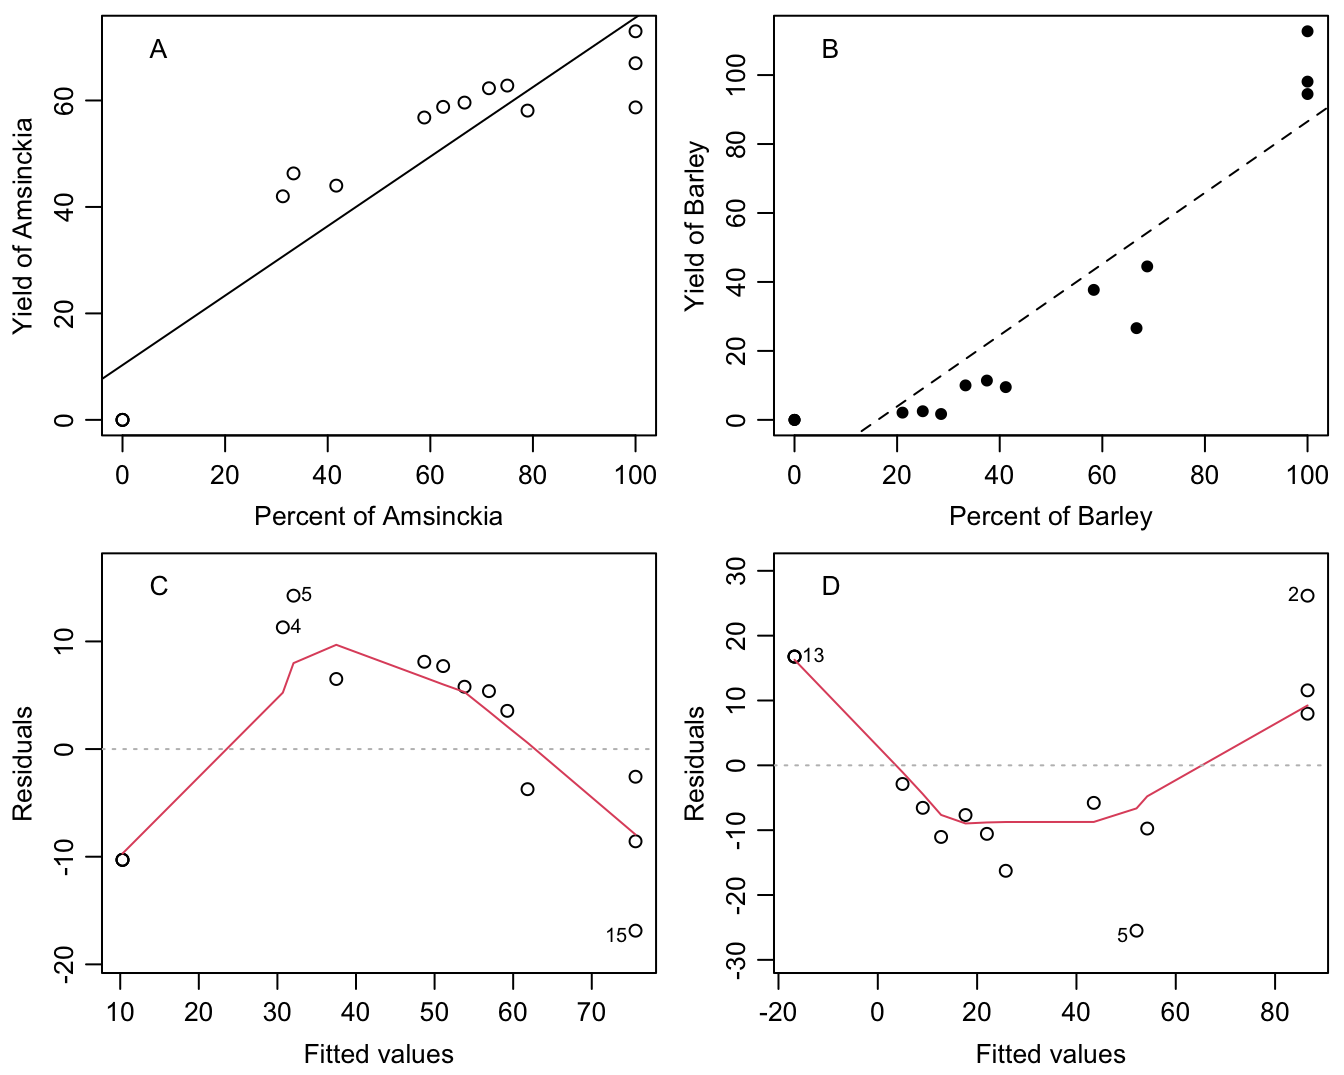
\includegraphics{Rstats4ag_files/figure-latex/figrelserlm-1.pdf}
\caption{\label{fig:figrelserlm}\emph{Straight line relationships do not appear to capture the variation in the species. The analysis of residuals shows systematic departure form the expected shotgun distribution of residuals.}}
\end{figure}

Obviously, the relationships in Figure \ref{fig:figrelserlm} for both species look like a curved relationship. We are not sure of which relationship to use and resort to a second degree polynomial.

\[Yield = a+bx+cx^2 .\]

where \emph{a} is the intercept with the y-axis and \emph{b} and \emph{c} are parameters for the \emph{x} and the \emph{x}\textsuperscript{2}.
The biological meanings of polynomial parameters in general are not often of interest because they can be hard to interpret. To fit the polynomial we use the \texttt{lm()}function because it is essentially a linear model we are fitting by adding a parameter for the \emph{x}\textsuperscript{2} by writing \texttt{I(x\^{}2)}. However, we cannot use the \texttt{abline()} function since there is now more than one `slope' parameter.

To plot a line, first we generate predicted values using the polynomial model to get smooth fits. It is done with the \texttt{predict()}function \texttt{predict(Pol.B.Amsinckia,data.frame(Pct.Amsinckia=seq(0,100,by=1)))}
where

\begin{itemize}
\tightlist
\item
  \texttt{Pol.B.Amsinckia} the results of the second degree polynomial fit for Amsinckia
\item
  \texttt{data.frame(Pct.Amsinckia=seq(0,100,by=1))} generates a sequence of `x' values from 0 to 100 by 1 (for a total of 101 values).
\end{itemize}

The same procedure applies to barley.



\begin{Shaded}
\begin{Highlighting}[]
\NormalTok{Pol.B.Amsinckia<-}\KeywordTok{lm}\NormalTok{(B.Amsinckia }\OperatorTok{~}\NormalTok{Pct.Amsinckia}\OperatorTok{+}\KeywordTok{I}\NormalTok{(Pct.Amsinckia}\OperatorTok{^}\DecValTok{2}\NormalTok{),}\DataTypeTok{data=}\NormalTok{Replace}\FloatTok{.1}\NormalTok{)}
\NormalTok{line.Pol.B.Amsinckia<-}\KeywordTok{predict}\NormalTok{(Pol.B.Amsinckia,}\KeywordTok{data.frame}\NormalTok{(}\DataTypeTok{Pct.Amsinckia=}\KeywordTok{seq}\NormalTok{(}\DecValTok{0}\NormalTok{,}\DecValTok{100}\NormalTok{,}\DataTypeTok{by=}\DecValTok{1}\NormalTok{)))}

\NormalTok{Pol.B.Barley<-}\KeywordTok{lm}\NormalTok{(B.Barley }\OperatorTok{~}\NormalTok{Pct.Barley}\OperatorTok{+}\KeywordTok{I}\NormalTok{(Pct.Barley}\OperatorTok{^}\DecValTok{2}\NormalTok{),}\DataTypeTok{data=}\NormalTok{Replace}\FloatTok{.1}\NormalTok{)}
\NormalTok{line.Pol.B.Barley<-}\KeywordTok{predict}\NormalTok{(Pol.B.Barley,}\KeywordTok{data.frame}\NormalTok{(}\DataTypeTok{Pct.Barley=}\KeywordTok{seq}\NormalTok{(}\DecValTok{0}\NormalTok{,}\DecValTok{100}\NormalTok{,}\DataTypeTok{by=}\DecValTok{1}\NormalTok{)))}

\KeywordTok{par}\NormalTok{(}\DataTypeTok{mfrow =} \KeywordTok{c}\NormalTok{(}\DecValTok{1}\NormalTok{, }\DecValTok{2}\NormalTok{), }\DataTypeTok{mar=}\KeywordTok{c}\NormalTok{(}\FloatTok{3.2}\NormalTok{,}\FloatTok{3.2}\NormalTok{,.}\DecValTok{5}\NormalTok{,.}\DecValTok{5}\NormalTok{), }\DataTypeTok{mgp=}\KeywordTok{c}\NormalTok{(}\DecValTok{2}\NormalTok{,.}\DecValTok{7}\NormalTok{,.}\DecValTok{0}\NormalTok{))}
\KeywordTok{plot}\NormalTok{(B.Amsinckia }\OperatorTok{~}\NormalTok{Pct.Amsinckia,}\DataTypeTok{data=}\NormalTok{Replace}\FloatTok{.1}\NormalTok{,}\DataTypeTok{ylim=}\KeywordTok{c}\NormalTok{(}\DecValTok{0}\NormalTok{,}\DecValTok{100}\NormalTok{), }\DataTypeTok{bty=}\StringTok{"l"}\NormalTok{,}
     \DataTypeTok{ylab=}\StringTok{"Amsinckia yield"}\NormalTok{, }\DataTypeTok{xlab=}\StringTok{"Percent Amsinckia"}\NormalTok{)}
\KeywordTok{lines}\NormalTok{(line.Pol.B.Amsinckia}\OperatorTok{~}\KeywordTok{seq}\NormalTok{(}\DecValTok{0}\NormalTok{,}\DecValTok{100}\NormalTok{,}\DataTypeTok{by=}\DecValTok{1}\NormalTok{),}\DataTypeTok{col=}\StringTok{"red"}\NormalTok{)}
\KeywordTok{plot}\NormalTok{(B.Barley }\OperatorTok{~}\NormalTok{Pct.Barley,}\DataTypeTok{data=}\NormalTok{Replace}\FloatTok{.1}\NormalTok{,}\DataTypeTok{pch=}\DecValTok{16}\NormalTok{,}\DataTypeTok{ylim=}\KeywordTok{c}\NormalTok{(}\DecValTok{0}\NormalTok{,}\DecValTok{100}\NormalTok{), }\DataTypeTok{bty=}\StringTok{"l"}\NormalTok{,}
     \DataTypeTok{ylab=}\StringTok{"Barley yield"}\NormalTok{, }\DataTypeTok{xlab=}\StringTok{"Percent Barley"}\NormalTok{)}
\KeywordTok{lines}\NormalTok{(line.Pol.B.Barley}\OperatorTok{~}\KeywordTok{seq}\NormalTok{(}\DecValTok{0}\NormalTok{,}\DecValTok{100}\NormalTok{,}\DataTypeTok{by=}\DecValTok{1}\NormalTok{),}\DataTypeTok{col=}\StringTok{"red"}\NormalTok{,}\DataTypeTok{lty=}\DecValTok{2}\NormalTok{)}
\end{Highlighting}
\end{Shaded}

\begin{figure}
\centering
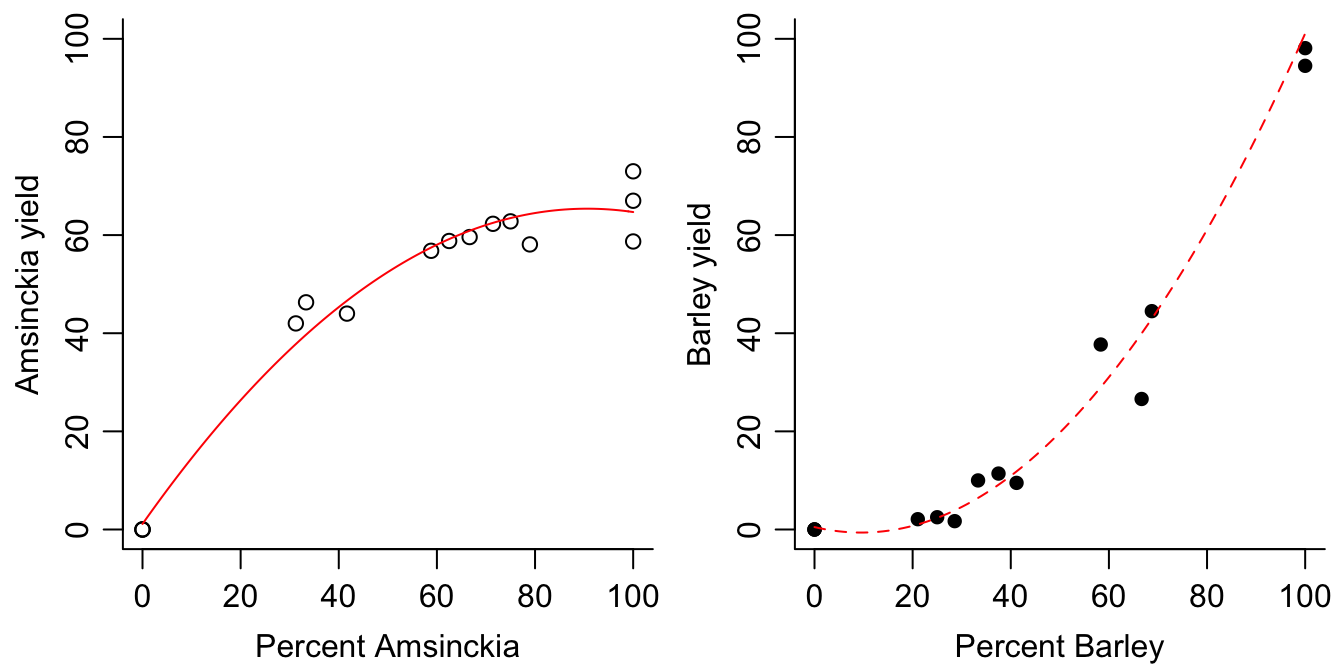
\includegraphics{Rstats4ag_files/figure-latex/figcomppoly-1.pdf}
\caption{\label{fig:figcomppoly}\emph{Fitting second degree polynomials to data.}}
\end{figure}

Overall the second degree polynomials describe the variation reasonably well (Figure \ref{fig:figcomppoly}). However, there is a catch to it, the minimum for the Amsinckia second degree polynomial is at low percent of Amsinckia and the maximum for the second degree polynomial for barley is at rather high proportion of barley. If we can live with that we can use the fit to summarize the experiment by calculation the Yield Total (\emph{YT}) as shown in the graph in Figure \ref{fig:figrepser}.

This is a good example of the problem with polynomials. A Second degree polynomial is symmetric with either a minimum or a maximum depending of the parameters. A third degree polynomial does not have this symmetric property, it becomes much more complex, and it is definitely not advisable to use with interpolations. In order to summarize the experiment on the basis of the fits, we can combine the two curves for the two species and calculate the \emph{YT}.

We want to use the \texttt{line.Pol.B.Amsinckia} and the \texttt{line.Pol.B.Barley} that define the smooth lines and calculate \emph{YT}. In order to calculate the YT we must sum the two predicted yields, but we must be carevul to reverse the order of one of the species (in this case we'll reverse using the function \texttt{rev(line.Pol.B.Barley)}. For this example, the maximum yield is 102, which occurs when the percentage of \emph{Amsinckia} is 0\% (found by using the \texttt{which.max()} function).



\begin{Shaded}
\begin{Highlighting}[]
\KeywordTok{max}\NormalTok{(line.Pol.B.Amsinckia }\OperatorTok{+}\StringTok{ }\KeywordTok{rev}\NormalTok{(line.Pol.B.Barley))}
\end{Highlighting}
\end{Shaded}

\begin{verbatim}
## [1] 102.2132
\end{verbatim}

\begin{Shaded}
\begin{Highlighting}[]
\KeywordTok{which.max}\NormalTok{(line.Pol.B.Amsinckia }\OperatorTok{+}\StringTok{ }\KeywordTok{rev}\NormalTok{(line.Pol.B.Barley))}\OperatorTok{-}\DecValTok{1}
\end{Highlighting}
\end{Shaded}

\begin{verbatim}
## 1 
## 0
\end{verbatim}

\begin{Shaded}
\begin{Highlighting}[]
\KeywordTok{par}\NormalTok{(}\DataTypeTok{mfrow =} \KeywordTok{c}\NormalTok{(}\DecValTok{1}\NormalTok{, }\DecValTok{1}\NormalTok{), }\DataTypeTok{mar=}\KeywordTok{c}\NormalTok{(}\FloatTok{5.2}\NormalTok{,}\FloatTok{3.2}\NormalTok{,}\FloatTok{0.5}\NormalTok{,.}\DecValTok{5}\NormalTok{), }\DataTypeTok{mgp=}\KeywordTok{c}\NormalTok{(}\DecValTok{2}\NormalTok{,.}\DecValTok{7}\NormalTok{,.}\DecValTok{0}\NormalTok{))}
\KeywordTok{plot}\NormalTok{(}\KeywordTok{c}\NormalTok{(line.Pol.B.Amsinckia[}\DecValTok{101}\NormalTok{],line.Pol.B.Barley[}\DecValTok{101}\NormalTok{])}\OperatorTok{~}\KeywordTok{c}\NormalTok{(}\DecValTok{100}\NormalTok{,}\DecValTok{0}\NormalTok{),}\DataTypeTok{type=}\StringTok{"l"}\NormalTok{,}
     \DataTypeTok{ylim=}\KeywordTok{c}\NormalTok{(}\DecValTok{0}\NormalTok{,}\DecValTok{120}\NormalTok{), }\DataTypeTok{xlab=}\StringTok{""}\NormalTok{, }\DataTypeTok{ylab=}\StringTok{"Yield"}\NormalTok{, }\DataTypeTok{bty=}\StringTok{"l"}\NormalTok{)}
\KeywordTok{mtext}\NormalTok{(}\StringTok{"Amsinckia (%) --->"}\NormalTok{,}\DataTypeTok{side=}\DecValTok{1}\NormalTok{,}\DataTypeTok{line=}\DecValTok{2}\NormalTok{)}
\KeywordTok{mtext}\NormalTok{(}\StringTok{"<--- Barley (100-%)"}\NormalTok{,}\DataTypeTok{side=}\DecValTok{1}\NormalTok{,}\DataTypeTok{line=}\DecValTok{3}\NormalTok{)}
\NormalTok{Pred.RYT<-line.Pol.B.Amsinckia[}\DecValTok{1}\OperatorTok{:}\DecValTok{101}\NormalTok{]}\OperatorTok{+}\NormalTok{line.Pol.B.Barley[}\KeywordTok{seq}\NormalTok{(}\DecValTok{101}\NormalTok{,}\DecValTok{1}\NormalTok{,}\DataTypeTok{by=}\OperatorTok{-}\DecValTok{1}\NormalTok{)]}
\KeywordTok{lines}\NormalTok{(Pred.RYT}\OperatorTok{~}\KeywordTok{seq}\NormalTok{(}\DecValTok{0}\NormalTok{,}\DecValTok{100}\NormalTok{,}\DataTypeTok{by=}\DecValTok{1}\NormalTok{),}\DataTypeTok{lty=}\DecValTok{3}\NormalTok{,}\DataTypeTok{lwd=}\DecValTok{2}\NormalTok{)}
\KeywordTok{lines}\NormalTok{(line.Pol.B.Barley}\OperatorTok{~}\KeywordTok{seq}\NormalTok{(}\DecValTok{100}\NormalTok{,}\DecValTok{0}\NormalTok{,}\DataTypeTok{by=}\OperatorTok{-}\DecValTok{1}\NormalTok{),}\DataTypeTok{col=}\StringTok{"blue"}\NormalTok{,}\DataTypeTok{lty=}\DecValTok{2}\NormalTok{)}
\KeywordTok{lines}\NormalTok{(line.Pol.B.Amsinckia}\OperatorTok{~}\KeywordTok{seq}\NormalTok{(}\DecValTok{0}\NormalTok{,}\DecValTok{100}\NormalTok{,}\DataTypeTok{by=}\DecValTok{1}\NormalTok{),}\DataTypeTok{col=}\StringTok{"red"}\NormalTok{,}\DataTypeTok{lty=}\DecValTok{1}\NormalTok{)}
\KeywordTok{points}\NormalTok{(B.Amsinckia }\OperatorTok{~}\NormalTok{Pct.Amsinckia,}\DataTypeTok{data=}\NormalTok{Replace}\FloatTok{.1}\NormalTok{,}\DataTypeTok{pch=}\DecValTok{19}\NormalTok{,}\DataTypeTok{ylim=}\KeywordTok{c}\NormalTok{(}\DecValTok{0}\NormalTok{,}\DecValTok{100}\NormalTok{), }\DataTypeTok{col=}\StringTok{"red"}\NormalTok{)}
\KeywordTok{points}\NormalTok{(B.Barley }\OperatorTok{~}\NormalTok{Pct.Amsinckia,}\DataTypeTok{data=}\NormalTok{Replace}\FloatTok{.1}\NormalTok{,}\DataTypeTok{pch=}\DecValTok{1}\NormalTok{,}\DataTypeTok{ylim=}\KeywordTok{c}\NormalTok{(}\DecValTok{0}\NormalTok{,}\DecValTok{100}\NormalTok{), }\DataTypeTok{col=}\StringTok{"blue"}\NormalTok{)}
\end{Highlighting}
\end{Shaded}

\begin{figure}
\centering
\includegraphics{Rstats4ag_files/figure-latex/figrepselYT-1.pdf}
\caption{\label{fig:figrepselYT}\emph{Summary of the replacement series experiment with barley and} Amsinckia. \emph{Solid and dotted black lines represent theoretical linear and estimated actual YT, respectively; red solid line and filled circles represent Amsinckia yield; blue dashed line and open circles represent barley yield.}}
\end{figure}

It seems in Figure \ref{fig:figrepselYT} that if Amsinckia gains with its convex curve, and barley suffers with its concave curve, but gain and suffering still leave the YT below the theoretical value of YT.

Another issue is that that we do not test the regressions statistically, but use the fit to illustrate the relationships. In order to apply test statistics it requires more systematic designs with fixed number of plants per unit area, which unfortunately was not the case here. In the first example we had genuine replication with several replicates of the number of volunteer corn per unit area and therefore we could test which model could be used.

It also shows that when fitting curves we can derive predicted values, which can be used to calculate derived parameters such as YT. In replacement series analysis, one often scales the results so that the theoretical maximum yield is equal to 1.0 and then calculate the Relative yield Total (RYT), which in mixed cropping research is called Land Equivalent Ratio (LER).

\begin{center}\rule{0.5\linewidth}{0.5pt}\end{center}

\hypertarget{seed-germination}{%
\chapter{Seed Germination}\label{seed-germination}}

Most weeds multiply and spread by seeds and understanding how seeds germinate, and how ambient factors affect seed dormancy, germination, vigor and early growth is instrumental for our continuous struggle to deplete soils of weed seeds. On agricultural land in Denmark we find about 30,000 viable weed seeds/m\^{}2. It has dropped to half of what we found 45 years ago. This drop is due to many factors, but probably the most important one is the continuous use of herbicides.

The weed's ability to set seed and the seeds' ability to germinate is therefore important for us to try understand and counteract seed soil bank enrichment with agronomic means. Therefore, seed testing experiments to assess germination ability and vigor should support future action of depleting weed pressure.

The International Seed Testing Association \href{https://www.seedtest.org/en/home.html}{ISTA} produces internationally agreed rules for seed sampling and testing and disseminates knowledge in seed science and technology. This facilitates seed trading nationally and internationally and is focusing on agricultural species. The principles of studying agricultural species and weed species are the same, but for weed species we are not interested in certifying their germinability, but to discover how to counteract their germination ability and vigor. In crop science and breeding the aim is the opposite to select for germinability and vigor.

Nonlinear regression is commonly used to evaluate cumulative germination in cause of time, temperature or other external gradients. This approach, however, is problematic as it ignores that successive observations on the germination curve are highly correlated. The total number of seeds that have germinated at a particular time is highly dependent on the number of seeds that already have germinated. Moreover, variation in the proportions of germinated seeds will vary with time, being largest at intermediate monitoring intervals and smallest at the initial and final intervals, where germination activity is low. This means that the fundamental assumptions implicitly underlying nonlinear regression (independence among proportions and variance homogeneity) are not met.

In experiments, where new batches of seed are used for each inspection time, data can be analyzed by well-established models for binomial data such as log-logistic regression or other generalized linear models.

In experiments where the same batch of seeds is followed over time, the same seeds are observed repeatedly for some pre-specified duration of an experiment. We observe the waiting time until the event of interest occurs and the resulting data are often referred to as event-time or time-to-event data.

In this chapter we will concentrate on time-to-event data \href{http://www.sciencedirect.com/science/article/pii/S1161030112001360}{Ritz et al.~2013}. Figure 14.1 shows the basic arrangement of this kind of experiment and how we arrange the data in R.

\begin{figure}
\centering
\includegraphics{Picture_petridish.png}
\caption{Example of how an experiment set up with four petridishes and how the data are arranged for being prepared for time-to-event analysis}
\end{figure}

For various reasons germination need not occur at all during the experiment. We refer to this as right-censoring. Consequently, a plausible statistical model has to incorporate that the event of interest, seed germination, may occur after termination of the experiment, assigning a positive probability to the situation that germination is not observed. This is why the final inspection time has an \texttt{Inf} value that means infinity concludes the experiment.

Also, the germination is obviously not observed exactly at the very point in time, when the event took place. For instance, seeds in petridishes may only be inspected on a daily or weekly basis and in case a seed has germinated the only information we get: because germination took place between two inspection intervals. This type of time-to-event data is often referred to as grouped data or interval-censored. As a consequence an appropriate model should be specified by means of the probability of germination within the monitoring intervals. This probability will depend heavily on the monitoring intervals. Ignoring this grouped-data structure may lead to biased estimates. The finer the time grid the smaller the error caused by ignoring discretization.

\hypertarget{example-1-chickweed}{%
\section{Example 1: Chickweed}\label{example-1-chickweed}}

\begin{Shaded}
\begin{Highlighting}[]
\KeywordTok{library}\NormalTok{(drc)}
\KeywordTok{head}\NormalTok{(chickweed,}\DecValTok{3}\NormalTok{)}
\end{Highlighting}
\end{Shaded}

\begin{verbatim}
##   start end count
## 1     0  12     0
## 2    12  22     0
## 3    22  30     0
\end{verbatim}

\begin{Shaded}
\begin{Highlighting}[]
\KeywordTok{tail}\NormalTok{(chickweed,}\DecValTok{3}\NormalTok{)}
\end{Highlighting}
\end{Shaded}

\begin{verbatim}
##    start   end count
## 33 266.5 276.5     1
## 34 276.5 281.5     0
## 35 281.5   Inf   160
\end{verbatim}

\begin{Shaded}
\begin{Highlighting}[]
\NormalTok{chickweed.m1 <-}\StringTok{ }\KeywordTok{drm}\NormalTok{(count}\OperatorTok{~}\NormalTok{start}\OperatorTok{+}\NormalTok{end, }\DataTypeTok{data =}\NormalTok{ chickweed, }\DataTypeTok{fct =} \KeywordTok{LL.3}\NormalTok{(}\DataTypeTok{names=}\KeywordTok{c}\NormalTok{(}\StringTok{"b"}\NormalTok{,}\StringTok{"MaxGerm"}\NormalTok{,}\StringTok{"T50"}\NormalTok{)), }\DataTypeTok{type =} \StringTok{"event"}\NormalTok{)}
\end{Highlighting}
\end{Shaded}

Notice the model \texttt{count\textasciitilde{}start+end} operates with two independent variables the \texttt{start} and \texttt{end}. It means that the intervals between inspection can vary; there is not need to have the same inspection intervals for the whole period of the experiment.

\begin{Shaded}
\begin{Highlighting}[]
\KeywordTok{summary}\NormalTok{(chickweed.m1)  }
\end{Highlighting}
\end{Shaded}

\begin{verbatim}
## 
## Model fitted: Log-logistic (ED50 as parameter) with lower limit at 0 (3 parms)
## 
## Parameter estimates:
## 
##                      Estimate Std. Error t-value   p-value    
## b:(Intercept)       -20.76747    2.94423 -7.0536 1.743e-12 ***
## MaxGerm:(Intercept)   0.20011    0.02830  7.0711 1.537e-12 ***
## T50:(Intercept)     196.05308    2.50570 78.2427 < 2.2e-16 ***
## ---
## Signif. codes:  0 '***' 0.001 '**' 0.01 '*' 0.05 '.' 0.1 ' ' 1
\end{verbatim}

The output from the \texttt{drm()}is the same as for other non-linear regressions, and the three parameter log-logistic model, \texttt{LL.3()}, is also familiar in dose-response work. What is new here is that the model needs \texttt{start+end,...,type\ =\ "event"}. The regression is illustrated in Figure \ref{fig:figgermchick}.



\begin{Shaded}
\begin{Highlighting}[]
\KeywordTok{par}\NormalTok{(}\DataTypeTok{mfrow=}\KeywordTok{c}\NormalTok{(}\DecValTok{1}\NormalTok{,}\DecValTok{1}\NormalTok{), }\DataTypeTok{mar=}\KeywordTok{c}\NormalTok{(}\FloatTok{3.6}\NormalTok{,}\FloatTok{3.6}\NormalTok{,.}\DecValTok{5}\NormalTok{,.}\DecValTok{5}\NormalTok{), }\DataTypeTok{mgp=}\KeywordTok{c}\NormalTok{(}\FloatTok{2.5}\NormalTok{,.}\DecValTok{7}\NormalTok{,}\DecValTok{0}\NormalTok{))}
\KeywordTok{plot}\NormalTok{(chickweed.m1, }\DataTypeTok{xlab =} \StringTok{"Time (hours)"}\NormalTok{, }\DataTypeTok{ylab =} \StringTok{"Proportion germinated"}\NormalTok{, }
     \DataTypeTok{xlim=}\KeywordTok{c}\NormalTok{(}\DecValTok{0}\NormalTok{, }\DecValTok{340}\NormalTok{), }\DataTypeTok{ylim=}\KeywordTok{c}\NormalTok{(}\DecValTok{0}\NormalTok{, }\FloatTok{0.25}\NormalTok{), }\DataTypeTok{log=}\StringTok{""}\NormalTok{, }\DataTypeTok{lwd=}\DecValTok{2}\NormalTok{, }\DataTypeTok{cex=}\FloatTok{1.2}\NormalTok{, }\DataTypeTok{bty=}\StringTok{"l"}\NormalTok{)  }
\end{Highlighting}
\end{Shaded}

\begin{figure}
\centering
\includegraphics{Rstats4ag_files/figure-latex/figgermchick-1.pdf}
\caption{\label{fig:figgermchick}\emph{Germination curves of ALS resistant} Stellaria media \emph{from Danish fields in 2001. The code is from the example data set chickweed in the \texttt{drc} package \href{http://www.sciencedirect.com/science/article/pii/S1161030112001360}{Ritz et al.~2013}. Note that we now use the actual time on the x-axis and not the logarithm as we did in the dose-response curve chapter.}}
\end{figure}

On the basis of the regression parameters we can see that the maximum germination rate is not that high and the \(T_{50}\) is 196 hours, meaning that it takes 196 days to reach 0.20/2= 0.1 or 10\% germination. The interesting biological parameters are the upper limit (maximum germination) 0.20 (0.03) and the time to 50\% germination, \(T_{50}\), 196 (2.5).

As was the case in the dose-response chapter we can also estimate how long it takes to reach 10 or 90 percent germination.

\begin{Shaded}
\begin{Highlighting}[]
\CommentTok{## Calculating t10, $T_\{50\}$, t90 for the distribution of viable seeds}
\KeywordTok{ED}\NormalTok{(chickweed.m1, }\KeywordTok{c}\NormalTok{(}\DecValTok{10}\NormalTok{, }\DecValTok{50}\NormalTok{, }\DecValTok{90}\NormalTok{), }\DataTypeTok{interval=}\StringTok{"delta"}\NormalTok{)}
\end{Highlighting}
\end{Shaded}

\begin{verbatim}
## 
## Estimated effective doses
## 
##        Estimate Std. Error    Lower    Upper
## e:1:10 176.3700     3.4930 169.5239 183.2161
## e:1:50 196.0531     2.5057 191.1420 200.9642
## e:1:90 217.9328     4.2730 209.5578 226.3078
\end{verbatim}

If a cumulative germination curve had been analysed by a nonlinear regressions, the parameters would be similar, but their standard errors would be overly precise. If we are interested only in the curve fitting and not the uncertainties of parameters, either way of fitting may suffice. But usually we want to get the correct standard error of parameters to compare germination ability and/or vigor among species, biotypes, or environments, and the time-to-event regression is the appropriate way to better estimate the uncertainty in germination estimates, and may prevent us from drawing incorrect conclusions.

\hypertarget{example-2-bromus-tectorum}{%
\section{\texorpdfstring{Example 2: \emph{Bromus tectorum}}{Example 2: Bromus tectorum}}\label{example-2-bromus-tectorum}}

Another example uses germination data for three different biotypes of \emph{Bromus tectorum} collected in Wyoming. Seeds were placed in petri dishes on moist filter paper in a germination chamber. The petri dishes were checked for germinated seeds once daily from the initiation of the experiment for 20 days. Each day the number of newly germinated seeds was recorded.

\begin{Shaded}
\begin{Highlighting}[]
\NormalTok{germ.dat<-}\KeywordTok{read.csv}\NormalTok{(}\StringTok{"http://rstats4ag.org/data/broteGerm.csv"}\NormalTok{)}
\KeywordTok{head}\NormalTok{(germ.dat,}\DecValTok{3}\NormalTok{)}
\end{Highlighting}
\end{Shaded}

\begin{verbatim}
##   Source starttime endtime REP Daily.germ Cum.Germ
## 1     S1         0       1   1          0        0
## 2     S1         0       1   2          0        0
## 3     S1         0       1   3          0        0
\end{verbatim}

There are 6 columns in the data set, the \texttt{Source} is the \emph{B. tectorum} biotype, \texttt{starttime} and \texttt{endtime} denote the beginning and end of the interval represented by each recording time. This is similar to the chickweed data set. The \texttt{Daily.germ} column represents the number of germination events that occurred since the last observation. The \texttt{Cum.germ} column is a cumulative total that is often used (incorrectly) for analyzing germination over time.

The final observation in this experiment occurred 20 days after it began. Therefore, we have an interval in the data set from time period 20 to \texttt{Inf}. Many of the petri dishes had not germinated all seeds at the final observation. We don't know for certain that these seeds \emph{never} would have germinated. All we can say is that they had not yet germinated at the final observation of day 20. In the data set, we incorporate this uncertainty by recording the number of non-germinated seeds in the interval 20 to \texttt{Inf}.



\begin{Shaded}
\begin{Highlighting}[]
\NormalTok{event.drc<-}\KeywordTok{drm}\NormalTok{(Daily.germ }\OperatorTok{~}\StringTok{ }\NormalTok{starttime}\OperatorTok{+}\NormalTok{endtime, Source, }\DataTypeTok{data=}\NormalTok{germ.dat, }
               \DataTypeTok{fct=}\KeywordTok{LL.3}\NormalTok{(}\DataTypeTok{names=}\KeywordTok{c}\NormalTok{(}\StringTok{"Slope"}\NormalTok{,}\StringTok{"Max"}\NormalTok{,}\StringTok{"T50"}\NormalTok{)), }\DataTypeTok{type=}\StringTok{"event"}\NormalTok{,}
               \DataTypeTok{upperl=}\KeywordTok{c}\NormalTok{(}\OtherTok{NA}\NormalTok{,}\DecValTok{1}\NormalTok{,}\OtherTok{NA}\NormalTok{))}
\KeywordTok{summary}\NormalTok{(event.drc)}
\end{Highlighting}
\end{Shaded}

\begin{verbatim}
## 
## Model fitted: Log-logistic (ED50 as parameter) with lower limit at 0 (3 parms)
## 
## Parameter estimates:
## 
##            Estimate Std. Error t-value   p-value    
## Slope:S1  -9.037575   0.673091 -13.427 < 2.2e-16 ***
## Slope:S2 -21.195415   1.478692 -14.334 < 2.2e-16 ***
## Slope:S3  -6.881944   0.487129 -14.128 < 2.2e-16 ***
## Max:S1     0.723603   0.031958  22.642 < 2.2e-16 ***
## Max:S2     0.861457   0.024301  35.449 < 2.2e-16 ***
## Max:S3     0.823935   0.027511  29.949 < 2.2e-16 ***
## T50:S1    11.159361   0.183671  60.757 < 2.2e-16 ***
## T50:S2    10.207564   0.067115 152.091 < 2.2e-16 ***
## T50:S3     9.481163   0.189789  49.956 < 2.2e-16 ***
## ---
## Signif. codes:  0 '***' 0.001 '**' 0.01 '*' 0.05 '.' 0.1 ' ' 1
\end{verbatim}

\begin{Shaded}
\begin{Highlighting}[]
\KeywordTok{par}\NormalTok{(}\DataTypeTok{mar=}\KeywordTok{c}\NormalTok{(}\FloatTok{3.6}\NormalTok{,}\FloatTok{3.6}\NormalTok{,.}\DecValTok{5}\NormalTok{,.}\DecValTok{5}\NormalTok{), }\DataTypeTok{mgp=}\KeywordTok{c}\NormalTok{(}\DecValTok{2}\NormalTok{,.}\DecValTok{7}\NormalTok{,}\DecValTok{0}\NormalTok{))}
\KeywordTok{plot}\NormalTok{(event.drc, }\DataTypeTok{log=}\StringTok{""}\NormalTok{, }\CommentTok{#ylim=c(0,1), xlim=c(0,20),  bty="l", }
     \DataTypeTok{ylab=}\StringTok{"Proportion of germinated seed"}\NormalTok{, }\DataTypeTok{xlab=}\StringTok{"Time (d)"}\NormalTok{,}
     \DataTypeTok{legendPos=}\KeywordTok{c}\NormalTok{(}\DecValTok{20}\NormalTok{,.}\DecValTok{40}\NormalTok{), }\DataTypeTok{pch=}\DecValTok{1}\OperatorTok{:}\DecValTok{3}\NormalTok{)}
\end{Highlighting}
\end{Shaded}

\begin{figure}
\centering
\includegraphics{Rstats4ag_files/figure-latex/figbrotegerm-1.pdf}
\caption{\label{fig:figbrotegerm}\emph{Regression fits for the time-to-event 3 parameter log-logistic regression. Please note that the curves for the time to event do stop at 20 days, because we do not know about future germination beyond 20 days.}}
\end{figure}

In this code, we have set the \texttt{names} argument within the \texttt{drc} fitting function \texttt{LL.3()}. By default, the three parameters are named \texttt{b,\ d}, and \texttt{e}. For users who deal with these models on a regular basis, it is certainly acceptable to leave the default parameter names and interpret them accordingly. However, renaming the parameters to \texttt{Slope}, \texttt{Max}, and \(T_{50}\) provides a useful reminder of how to interpret the parameters in the model output. This is especially helpful when presenting the results to someone unfamiliar with \texttt{R} syntax.

In germination studies, all three parameters have some biological interpretation. The upper limit being the maximal germination, with an upper limit set at 1 (or 100\% of the seed); \(T_{50}\) is the time taken to reach 50\% germination relative to the upper limit. The slope could give an indication of how quickly seed germination reaches completion once the process has begun. The \(T_{5}\) or \(T_{95}\) (the time required for 5 and 95 percent of the seeds to germinate, respectively) can also be estimated in relation to the upper limit.

\begin{Shaded}
\begin{Highlighting}[]
\CommentTok{#The ED5,ED50,and ED95 for the the germination}
\KeywordTok{ED}\NormalTok{(event.drc,}\KeywordTok{c}\NormalTok{(}\DecValTok{5}\NormalTok{,}\DecValTok{50}\NormalTok{,}\DecValTok{95}\NormalTok{), }\DataTypeTok{interval=}\StringTok{"delta"}\NormalTok{)}
\end{Highlighting}
\end{Shaded}

\begin{verbatim}
## 
## Estimated effective doses
## 
##          Estimate Std. Error     Lower     Upper
## e:S1:5   8.056499   0.223117  7.619198  8.493799
## e:S1:50 11.159361   0.183671 10.799373 11.519350
## e:S1:95 15.457253   0.477020 14.522312 16.392194
## e:S2:5   8.883630   0.102078  8.683561  9.083700
## e:S2:50 10.207564   0.067115 10.076021 10.339106
## e:S2:95 11.728803   0.139904 11.454596 12.003010
## e:S3:5   6.180858   0.216678  5.756177  6.605539
## e:S3:50  9.481163   0.189789  9.109183  9.853142
## e:S3:95 14.543684   0.545492 13.474539 15.612829
\end{verbatim}

Usually the \(T_{50}\) is the most precise estimate, this does also apply here when we look at the 95\% confidence interval or the coefficient of variation.

\begin{Shaded}
\begin{Highlighting}[]
\CommentTok{#Coefficient of variation for ED50}
\NormalTok{T50<-}\KeywordTok{ED}\NormalTok{(event.drc,}\KeywordTok{c}\NormalTok{(}\DecValTok{50}\NormalTok{),}\DataTypeTok{display=}\OtherTok{FALSE}\NormalTok{)[,}\DecValTok{2}\NormalTok{]}\OperatorTok{*}\DecValTok{100}\OperatorTok{/}\KeywordTok{ED}\NormalTok{(event.drc,}\KeywordTok{c}\NormalTok{(}\DecValTok{50}\NormalTok{),}\DataTypeTok{display=}\OtherTok{FALSE}\NormalTok{)[,}\DecValTok{1}\NormalTok{]}
\NormalTok{T50}
\end{Highlighting}
\end{Shaded}

\begin{verbatim}
##   e:S1:50   e:S2:50   e:S3:50 
## 1.6458918 0.6574998 2.0017478
\end{verbatim}

\begin{Shaded}
\begin{Highlighting}[]
\CommentTok{#Coefficient of variation for ED5}
\NormalTok{T5<-}\KeywordTok{ED}\NormalTok{(event.drc,}\KeywordTok{c}\NormalTok{(}\DecValTok{5}\NormalTok{),}\DataTypeTok{display=}\OtherTok{FALSE}\NormalTok{)[,}\DecValTok{2}\NormalTok{]}\OperatorTok{*}\DecValTok{100}\OperatorTok{/}\KeywordTok{ED}\NormalTok{(event.drc,}\KeywordTok{c}\NormalTok{(}\DecValTok{5}\NormalTok{),}\DataTypeTok{display=}\OtherTok{FALSE}\NormalTok{)[,}\DecValTok{1}\NormalTok{]}
\NormalTok{T5}
\end{Highlighting}
\end{Shaded}

\begin{verbatim}
##   e:S1:5   e:S2:5   e:S3:5 
## 2.769398 1.149057 3.505629
\end{verbatim}

\begin{Shaded}
\begin{Highlighting}[]
\CommentTok{#Coefficient of variation for ED95}
\NormalTok{T95<-}\KeywordTok{ED}\NormalTok{(event.drc,}\KeywordTok{c}\NormalTok{(}\DecValTok{95}\NormalTok{),}\DataTypeTok{display=}\OtherTok{FALSE}\NormalTok{)[,}\DecValTok{2}\NormalTok{]}\OperatorTok{*}\DecValTok{100}\OperatorTok{/}\KeywordTok{ED}\NormalTok{(event.drc,}\KeywordTok{c}\NormalTok{(}\DecValTok{95}\NormalTok{),}\DataTypeTok{display=}\OtherTok{FALSE}\NormalTok{)[,}\DecValTok{1}\NormalTok{]}
\NormalTok{T95}
\end{Highlighting}
\end{Shaded}

\begin{verbatim}
##  e:S1:95  e:S2:95  e:S3:95 
## 3.086056 1.192825 3.750715
\end{verbatim}

Direct comparison of model parameters can be done by using the \texttt{compParm()} function in \texttt{drc}. Because we have used the \texttt{names} argument above, we need to specify those names in the \texttt{compParm()} syntax. If we had not used the \texttt{names} argument, we would compare slopes by specifying the \emph{b} parameter, maximum asymptote \emph{d} parameter, and \(T_{50}\) the \emph{e} parameter.

\begin{Shaded}
\begin{Highlighting}[]
\KeywordTok{compParm}\NormalTok{(event.drc, }\StringTok{"Slope"}\NormalTok{)}
\end{Highlighting}
\end{Shaded}

\begin{verbatim}
## 
## Comparison of parameter 'Slope' 
## 
##       Estimate Std. Error  t-value   p-value    
## S1/S2 0.426393   0.043513 -13.1825 < 2.2e-16 ***
## S1/S3 1.313230   0.134932   2.3214   0.02027 *  
## S2/S3 3.079859   0.306093   6.7949 1.084e-11 ***
## ---
## Signif. codes:  0 '***' 0.001 '**' 0.01 '*' 0.05 '.' 0.1 ' ' 1
\end{verbatim}

Slopes are different between S2 and the rest as also seen in Figure \ref{fig:figbrotegerm}. It means that the vigor of the germination process for S3 is greater that for the other two biotypes. Looking at the upper limit:

\begin{Shaded}
\begin{Highlighting}[]
\KeywordTok{compParm}\NormalTok{(event.drc, }\StringTok{"Max"}\NormalTok{)}
\end{Highlighting}
\end{Shaded}

\begin{verbatim}
## 
## Comparison of parameter 'Max' 
## 
##       Estimate Std. Error t-value   p-value    
## S1/S2 0.839976   0.044020 -3.6353 0.0002777 ***
## S1/S3 0.878229   0.048625 -2.5043 0.0122691 *  
## S2/S3 1.045540   0.045702  0.9965 0.3190268    
## ---
## Signif. codes:  0 '***' 0.001 '**' 0.01 '*' 0.05 '.' 0.1 ' ' 1
\end{verbatim}

The maximum germination for biotypes S2 and S3 is similar, but biotype S1 has a lower maximum germination than do the other two biotypes. Finally, the time required for 50\% germination can also be compared in a similar manner.

\begin{Shaded}
\begin{Highlighting}[]
\KeywordTok{compParm}\NormalTok{(event.drc, }\StringTok{"T50"}\NormalTok{)}
\end{Highlighting}
\end{Shaded}

\begin{verbatim}
## 
## Comparison of parameter 'T50' 
## 
##       Estimate Std. Error t-value   p-value    
## S1/S2 1.093244   0.019376  4.8123 1.492e-06 ***
## S1/S3 1.177003   0.030502  5.8030 6.515e-09 ***
## S2/S3 1.076615   0.022684  3.3775 0.0007314 ***
## ---
## Signif. codes:  0 '***' 0.001 '**' 0.01 '*' 0.05 '.' 0.1 ' ' 1
\end{verbatim}

The \(T_{50}\) (which is also be associated with speed of germination) are different form each other. Looking at Figure \ref{fig:figbrotegerm}, it is noted that the logistic regression does not seem to be that good to capture the upper limits for S2 and S3, and perhaps the symmetric sigmoid curves would could be replaced by an asymmetric one. By using the Weibull 1 model, \texttt{W1.3()}, which is asymmetric (i.e. \(T_{50}\) is not a parameter in the model). We may be better to model the upper limit. However, the Weibull 1 is rather sensitive to too many zeros so we must get rid of those in order to get a proper fit.This is done by omitting observations with the functions \texttt{subset(germ.dat,\ Daily.germ!=0)}. This function gives some warnings that we can ignore for the time being.

\begin{Shaded}
\begin{Highlighting}[]
\CommentTok{#Fitting LL.3() with the same conditions as for the Weilbull 1 model}
\NormalTok{event.drc}\FloatTok{.1}\NormalTok{<-}\KeywordTok{drm}\NormalTok{(Daily.germ }\OperatorTok{~}\StringTok{ }\NormalTok{starttime}\OperatorTok{+}\NormalTok{endtime, Source, }
                 \DataTypeTok{fct=}\KeywordTok{LL.3}\NormalTok{(}\DataTypeTok{names=}\KeywordTok{c}\NormalTok{(}\StringTok{"Slope"}\NormalTok{,}\StringTok{"Max"}\NormalTok{,}\StringTok{"T50"}\NormalTok{)),}
                 \DataTypeTok{data=}\KeywordTok{subset}\NormalTok{(germ.dat, Daily.germ}\OperatorTok{!=}\DecValTok{0}\NormalTok{), }\DataTypeTok{type=}\StringTok{"event"}\NormalTok{)}

\CommentTok{#Fitting W1.3()}
\NormalTok{event.drc.W1 <-}\StringTok{ }\KeywordTok{drm}\NormalTok{(Daily.germ }\OperatorTok{~}\StringTok{ }\NormalTok{starttime}\OperatorTok{+}\NormalTok{endtime, Source, }
                    \DataTypeTok{fct=}\KeywordTok{W1.3}\NormalTok{(), }
                    \DataTypeTok{data=}\KeywordTok{subset}\NormalTok{(germ.dat, Daily.germ}\OperatorTok{!=}\DecValTok{0}\NormalTok{), }\DataTypeTok{type=}\StringTok{"event"}\NormalTok{)}

\CommentTok{#To extract the T50}
\KeywordTok{ED}\NormalTok{(event.drc}\FloatTok{.1}\NormalTok{,}\DecValTok{50}\NormalTok{) }\CommentTok{# LL.3 model}
\end{Highlighting}
\end{Shaded}

\begin{verbatim}
## 
## Estimated effective doses
## 
##          Estimate Std. Error
## e:S1:50 11.159333   0.183699
## e:S2:50 10.207537   0.067106
## e:S3:50  9.481139   0.189743
\end{verbatim}

\begin{Shaded}
\begin{Highlighting}[]
\KeywordTok{ED}\NormalTok{(event.drc.W1,}\DecValTok{50}\NormalTok{) }\CommentTok{# W1.3 model}
\end{Highlighting}
\end{Shaded}

\begin{verbatim}
## 
## Estimated effective doses
## 
##          Estimate Std. Error
## e:S1:50 11.043969   0.183815
## e:S2:50 10.151655   0.061806
## e:S3:50  9.352818   0.211253
\end{verbatim}

The \(T_{50}\) did not change much but in Figure \ref{fig:figbrotew}, there are subtle changes in the curve on the right side by going from a log-logistic \texttt{(LL.3())} to an asymmetric \texttt{(W1.3())} curve. There are some differences in the way the upper limit is described by the two models. The Weibull 1 seems to do a better job than the log-logistic.



\begin{Shaded}
\begin{Highlighting}[]
\KeywordTok{par}\NormalTok{(}\DataTypeTok{mfrow=}\KeywordTok{c}\NormalTok{(}\DecValTok{1}\NormalTok{,}\DecValTok{1}\NormalTok{), }\DataTypeTok{mar=}\KeywordTok{c}\NormalTok{(}\FloatTok{3.2}\NormalTok{,}\FloatTok{3.2}\NormalTok{,}\FloatTok{0.5}\NormalTok{,}\FloatTok{0.5}\NormalTok{), }\DataTypeTok{mgp=}\KeywordTok{c}\NormalTok{(}\DecValTok{2}\NormalTok{,.}\DecValTok{7}\NormalTok{,}\DecValTok{0}\NormalTok{))}
\KeywordTok{plot}\NormalTok{(event.drc.W1, }\DataTypeTok{log=}\StringTok{""}\NormalTok{, }\DataTypeTok{ylim=}\KeywordTok{c}\NormalTok{(}\DecValTok{0}\NormalTok{,}\DecValTok{1}\NormalTok{), }\DataTypeTok{xlim=}\KeywordTok{c}\NormalTok{(}\DecValTok{0}\NormalTok{,}\DecValTok{20}\NormalTok{), }\DataTypeTok{bty=}\StringTok{"l"}\NormalTok{,}
     \DataTypeTok{ylab=}\StringTok{"Proportion of germinated seed"}\NormalTok{, }\DataTypeTok{xlab=}\StringTok{"Time (d)"}\NormalTok{,}
     \DataTypeTok{legendPos=}\KeywordTok{c}\NormalTok{(}\DecValTok{20}\NormalTok{,.}\DecValTok{40}\NormalTok{))}
\KeywordTok{plot}\NormalTok{(event.drc}\FloatTok{.1}\NormalTok{, }\DataTypeTok{log=}\StringTok{""}\NormalTok{, }\DataTypeTok{ylim=}\KeywordTok{c}\NormalTok{(}\DecValTok{0}\NormalTok{,}\DecValTok{1}\NormalTok{), }\DataTypeTok{xlim=}\KeywordTok{c}\NormalTok{(}\DecValTok{0}\NormalTok{,}\DecValTok{20}\NormalTok{),   }
     \DataTypeTok{type=}\StringTok{"none"}\NormalTok{,}
     \DataTypeTok{add=}\OtherTok{TRUE}\NormalTok{, }\DataTypeTok{col=}\KeywordTok{c}\NormalTok{(}\DecValTok{2}\NormalTok{), }\DataTypeTok{legendPos=}\KeywordTok{c}\NormalTok{(}\DecValTok{20}\NormalTok{,.}\DecValTok{40}\NormalTok{))}
\end{Highlighting}
\end{Shaded}

\begin{figure}
\centering
\includegraphics{Rstats4ag_files/figure-latex/figbrotew-1.pdf}
\caption{\label{fig:figbrotew}\emph{An assymetric Weilbull 1 model(\texttt{W1.3()}) shown with black lines, compared with the symmetric log-logistic model (\texttt{LL.3()}) in red.}}
\end{figure}

Even though the changes are not dramatic the AIC does drop somewhat when going form a log-logistic to an Weibull 1, which indicates that overall the asymmetric \texttt{W1.3()} fits best to the data.

\begin{Shaded}
\begin{Highlighting}[]
\KeywordTok{AIC}\NormalTok{(event.drc}\FloatTok{.1}\NormalTok{, event.drc.W1)}
\end{Highlighting}
\end{Shaded}

\begin{verbatim}
##              df      AIC
## event.drc.1  79 2600.177
## event.drc.W1 79 2526.731
\end{verbatim}

\begin{center}\rule{0.5\linewidth}{0.5pt}\end{center}

\hypertarget{visualization}{%
\chapter{Visualization}\label{visualization}}

Pictures and graphs may say more than 1000 words. After collection of data, the hard work of analyzing them according to the experimental design plans begins. But before you dig too much into statistics and jump to conclusions on the basis of the statistical tests, you should actually look at the data graphically. You must try to illustrate the data in such a way that it is informative not only to you, but also to potential readers of the project or the paper you wish to publish. In a way you could look at the visualization as the interface between science and art. One of the best examples of this merger of science and art is the campaign of Napoleon in Russia 1812-1813.

\begin{figure}
\centering
\includegraphics{minardodt.png}
\caption{\label{fig:minardPlot}\emph{Charles Joseph Minard (1781-1870) is most widely known for a single work, his illustration of the fate of Napoleon's Grand Army in Russia.} Source: \url{http://www.datavis.ca/gallery/re-minard.php}}
\end{figure}

Minard's work (Figure \ref{fig:minardPlot}) has been called one of the best graphs ever produced in thematic cartography and statistical graphics. In short, it shows the size of the Army at the beginning of the attack and at the final retreat, some of the more important battles and the temperature during the retreat from Moscow. It contains so many dimensions and so much information and history that usually fill hundreds of pages in history books. Our work in weed science is rarely that exciting for the general public; although our discipline can be an esoteric at times, it plays a great role in the food production and sustainability of the farming and environment in the world.

\hypertarget{base-r-graphics}{%
\section{Base R Graphics}\label{base-r-graphics}}

Visualization of data is an important step to get a first impression of the quality of data and to see if some observations stand out from the rest. It can also help us observe whether the data show systematic relationships. Base R graphics are a quick and extensible way to do both this preliminary data inspection, but also for creating publication quality figures for manuscripts and presentations. We will begin this chapter with some basic examples of how to customize base R graphics to create high-quality figures.

\hypertarget{scatterplots}{%
\subsection{Scatterplots}\label{scatterplots}}

One of the most common figures is a scatter plot or x-y plot - typically used to see the relationship between an independent variable (x-axis) and a response variable (y-axis), although often used to show other relationships as well. Without much work, we can get a very simple scatterplot suitable for inspecting the data in the \texttt{cars} data set that is part of the base \texttt{R} installation (Figure \ref{fig:scatter1}).

\begin{quote}
Code to produce Figure \ref{fig:scatter1}:
\end{quote}

\begin{Shaded}
\begin{Highlighting}[]
\KeywordTok{plot}\NormalTok{(dist }\OperatorTok{~}\StringTok{ }\NormalTok{speed, }\DataTypeTok{data =}\NormalTok{ cars, }\DataTypeTok{main=}\StringTok{"Recorded in the 1920's"}\NormalTok{)}
\end{Highlighting}
\end{Shaded}

\begin{figure}
\centering
\includegraphics{Rstats4ag_files/figure-latex/scatter1-1.pdf}
\caption{\label{fig:scatter1}\emph{A most basic scatterplot in R, showing the speed of cars and the distance required for the car to stop. The tilde \textasciitilde{} can be difficult to find on some keyboards, depending on you language, but it is the defined ASCII code 126. In Windows you can press the ALT key, activate Num. Lock and press 126.}}
\end{figure}

While Figure \ref{fig:scatter1} is adequate for preliminary inspection of one's own data, it is woefully insufficient for submission to a journal. We can improve the figure greatly by making some simple additions to the basic plot code. To create Figure \ref{fig:scatter2}, the \texttt{par()} function is called to change some of the default graphing parameters. In this case we adjust the margins so that the bottom and left margins are set to 3.2, the top and right margins are set to 0.5. We have removed the main title (since that information would typically be contained in a figure caption according to most journal instructions), and also adjusted the axis labels, by setting them closer to the axis compared to default values using \texttt{mgp}. The \texttt{mgp} argument requires 3 numbers, which set the distance from the axis for the axis title, axis labels, and axis line, respectively. The defaults for \texttt{mgp} are 3, 1, 0 - so in this code we've removed some of the axis white space by moving the labels closer to the axis. We have also added axis labels and a main title, changed the plotting character (\texttt{pch=19}, which is a closed circle), and added some transparency to the points using the \texttt{rgb()} function and the \texttt{alpha} argument. Finally, we have, adjusted the x-axis to include 0, and removed the box around the figure by setting \texttt{bty="n"}. Setting \texttt{bty="l"} will leave the bottom and left lines of the box, and \texttt{bty="o"} will plot the entire box (the default).

\begin{quote}
Code to produce Figure \ref{fig:scatter2}:
\end{quote}

\begin{Shaded}
\begin{Highlighting}[]
\KeywordTok{par}\NormalTok{(}\DataTypeTok{mar=}\KeywordTok{c}\NormalTok{(}\FloatTok{3.2}\NormalTok{,}\FloatTok{3.2}\NormalTok{,}\FloatTok{0.5}\NormalTok{,.}\DecValTok{5}\NormalTok{), }\DataTypeTok{mgp=}\KeywordTok{c}\NormalTok{(}\DecValTok{2}\NormalTok{,.}\DecValTok{7}\NormalTok{,}\DecValTok{0}\NormalTok{))}
\KeywordTok{plot}\NormalTok{(dist }\OperatorTok{~}\StringTok{ }\NormalTok{speed, }\DataTypeTok{data =}\NormalTok{ cars,}
     \DataTypeTok{xlab=}\StringTok{"Speed of car (mph)"}\NormalTok{, }
     \DataTypeTok{ylab=}\StringTok{"Distance required to stop (ft)"}\NormalTok{,}
     \DataTypeTok{pch=}\DecValTok{19}\NormalTok{, }\DataTypeTok{col=}\KeywordTok{rgb}\NormalTok{(}\DataTypeTok{red=}\NormalTok{.}\DecValTok{3}\NormalTok{, }\DataTypeTok{blue=}\NormalTok{.}\DecValTok{3}\NormalTok{, }\DataTypeTok{green=}\NormalTok{.}\DecValTok{3}\NormalTok{, }\DataTypeTok{alpha=}\FloatTok{0.7}\NormalTok{),}
     \DataTypeTok{bty=}\StringTok{"n"}\NormalTok{, }\DataTypeTok{xlim=}\KeywordTok{c}\NormalTok{(}\DecValTok{0}\NormalTok{,}\DecValTok{25}\NormalTok{))}
\end{Highlighting}
\end{Shaded}

\begin{figure}
\centering
\includegraphics{Rstats4ag_files/figure-latex/scatter2-1.pdf}
\caption{\label{fig:scatter2}\emph{An improved scatter plot showing the cars data.}}
\end{figure}

\hypertarget{box-and-whisker-plots}{%
\subsection{Box and Whisker Plots}\label{box-and-whisker-plots}}

If we have some data where the ``treatment'' is not based upon a continuous x variable, then we can illustrate the variation with a boxplot. The data for this example \texttt{InsectSprays} are also included with the basic R installation.

\begin{quote}
Code to produce Figure \ref{fig:boxjitter}:
\end{quote}

\begin{Shaded}
\begin{Highlighting}[]
\KeywordTok{par}\NormalTok{(}\DataTypeTok{mfrow =} \KeywordTok{c}\NormalTok{(}\DecValTok{1}\NormalTok{,}\DecValTok{2}\NormalTok{), }\DataTypeTok{mar=}\KeywordTok{c}\NormalTok{(}\FloatTok{3.2}\NormalTok{,}\FloatTok{3.2}\NormalTok{,.}\DecValTok{5}\NormalTok{,.}\DecValTok{5}\NormalTok{), }\DataTypeTok{mgp=}\KeywordTok{c}\NormalTok{(}\DecValTok{2}\NormalTok{,.}\DecValTok{7}\NormalTok{,}\DecValTok{0}\NormalTok{))}
\KeywordTok{plot}\NormalTok{(count }\OperatorTok{~}\StringTok{ }\NormalTok{spray, }\DataTypeTok{data =}\NormalTok{ InsectSprays)}
  \KeywordTok{legend}\NormalTok{(}\StringTok{"topleft"}\NormalTok{,}\StringTok{"(a)"}\NormalTok{, }\DataTypeTok{bty=}\StringTok{"n"}\NormalTok{)}
\KeywordTok{plot}\NormalTok{(count }\OperatorTok{~}\StringTok{ }\KeywordTok{as.numeric}\NormalTok{(spray), }\DataTypeTok{data =}\NormalTok{ InsectSprays, }\DataTypeTok{pch=}\DecValTok{19}\NormalTok{)}
  \KeywordTok{legend}\NormalTok{(}\StringTok{"topleft"}\NormalTok{,}\StringTok{"(b)"}\NormalTok{, }\DataTypeTok{bty=}\StringTok{"n"}\NormalTok{)}
\end{Highlighting}
\end{Shaded}

\begin{figure}
\centering
\includegraphics{Rstats4ag_files/figure-latex/boxjitter-1.pdf}
\caption{\label{fig:boxjitter}\emph{Counts of insects in agricultural experimental units treated with different insecticides.}}
\end{figure}

Figure \ref{fig:boxjitter} illustrates how the default \texttt{plot()} function works in R; if the x-axis is based on factors (A through F) you automatically get a boxplot (Figure \ref{fig:boxjitter}a), where the median and the quartiles are shown, as well as an indication of extreme observations. On the other hand, if we convert the factors A through F to numerical values of x by using function \texttt{as.numeric()}, we get an ordinary continuous x variable (Figure \ref{fig:boxjitter}b). Factor A becomes 1 and factor B becomes 2 and so on. In this particular data we can change the names (e.g., F is becoming A and A becoming F) of the various sprays and it will just change the order on the x-axis. In doing so it could have a great influence on perceived relationship.

It is possible to combine these two panels in Figure \ref{fig:boxjitter} into a single panel, to more concisely show a high level of detail on the variance within and among treatments. To do so, we modify the code for Figure \ref{fig:boxjitter} by using \texttt{points()} instead of \texttt{plot()} for the second plot so that the points are added to the first plot instead of creating a new plotting space; jittering the points, or offsetting them slightly, in the `x' direction so that counts that are similar or the same can be more easily seen; adding some transparency to the points so that we can see if multiple points are on top of one another; and by removing the outlier points from the initial boxplot since all points will be added later.

\begin{quote}
Code to produce Figure \ref{fig:boxjitter2}:
\end{quote}

\begin{Shaded}
\begin{Highlighting}[]
\KeywordTok{par}\NormalTok{(}\DataTypeTok{mfrow =} \KeywordTok{c}\NormalTok{(}\DecValTok{1}\NormalTok{,}\DecValTok{1}\NormalTok{), }\DataTypeTok{mar=}\KeywordTok{c}\NormalTok{(}\FloatTok{3.2}\NormalTok{,}\FloatTok{3.2}\NormalTok{,.}\DecValTok{5}\NormalTok{,.}\DecValTok{5}\NormalTok{), }\DataTypeTok{mgp=}\KeywordTok{c}\NormalTok{(}\DecValTok{2}\NormalTok{,.}\DecValTok{7}\NormalTok{,}\DecValTok{0}\NormalTok{))}
\KeywordTok{plot}\NormalTok{(count }\OperatorTok{~}\StringTok{ }\NormalTok{spray, }\DataTypeTok{data =}\NormalTok{ InsectSprays, }\DataTypeTok{pch=}\OtherTok{NA}\NormalTok{)}
\KeywordTok{points}\NormalTok{(count }\OperatorTok{~}\StringTok{ }\KeywordTok{jitter}\NormalTok{(}\KeywordTok{as.numeric}\NormalTok{(spray)), }\DataTypeTok{data =}\NormalTok{ InsectSprays,}
       \DataTypeTok{pch=}\DecValTok{19}\NormalTok{, }\DataTypeTok{col=}\KeywordTok{rgb}\NormalTok{(.}\DecValTok{1}\NormalTok{,.}\DecValTok{4}\NormalTok{,.}\DecValTok{8}\NormalTok{, }\DataTypeTok{alpha=}\FloatTok{0.7}\NormalTok{))}
\end{Highlighting}
\end{Shaded}

\begin{figure}
\centering
\includegraphics{Rstats4ag_files/figure-latex/boxjitter2-1.pdf}
\caption{\label{fig:boxjitter2}\emph{Counts of insects in agricultural experimental units treated with different insecticides - shown with points on top of the boxplots.}}
\end{figure}

For data with continuous x we can also directly call the \texttt{boxplot()} function rather than relying on \texttt{R} to correctly identify the independent variable type. We can also use some additional arguments within the \texttt{boxplot()} function to modify the look of our boxplot (Figure \ref{fig:horizbox}).

\begin{quote}
Code to produce Figure \ref{fig:horizbox}:
\end{quote}

\begin{Shaded}
\begin{Highlighting}[]
\KeywordTok{par}\NormalTok{(}\DataTypeTok{mfrow =} \KeywordTok{c}\NormalTok{(}\DecValTok{1}\NormalTok{,}\DecValTok{1}\NormalTok{), }\DataTypeTok{mar=}\KeywordTok{c}\NormalTok{(}\FloatTok{3.2}\NormalTok{,}\FloatTok{8.2}\NormalTok{,.}\DecValTok{5}\NormalTok{,.}\DecValTok{5}\NormalTok{), }\DataTypeTok{mgp=}\KeywordTok{c}\NormalTok{(}\DecValTok{2}\NormalTok{,.}\DecValTok{7}\NormalTok{,}\DecValTok{0}\NormalTok{))}
\KeywordTok{boxplot}\NormalTok{(count }\OperatorTok{~}\StringTok{ }\KeywordTok{as.numeric}\NormalTok{(spray), }\DataTypeTok{data =}\NormalTok{ InsectSprays, }\DataTypeTok{horizontal=}\OtherTok{TRUE}\NormalTok{, }\DataTypeTok{pch=}\OtherTok{NA}\NormalTok{,}
        \DataTypeTok{names=}\KeywordTok{c}\NormalTok{(}\StringTok{"Antibug"}\NormalTok{,}\StringTok{"Bug Kill"}\NormalTok{,}\StringTok{"Clear"}\NormalTok{,}\StringTok{"Destroy"}\NormalTok{,}\StringTok{"Endgame"}\NormalTok{,}\StringTok{"Fuhgeddaboudit"}\NormalTok{),}
        \DataTypeTok{las=}\DecValTok{1}\NormalTok{, }\DataTypeTok{xlab=}\StringTok{"Insect counts"}\NormalTok{, }\DataTypeTok{ylab=}\StringTok{""}\NormalTok{)}
\KeywordTok{points}\NormalTok{(}\KeywordTok{jitter}\NormalTok{(}\KeywordTok{as.numeric}\NormalTok{(spray)) }\OperatorTok{~}\StringTok{ }\NormalTok{count, }\DataTypeTok{data =}\NormalTok{ InsectSprays,}
       \DataTypeTok{pch=}\DecValTok{19}\NormalTok{, }\DataTypeTok{col=}\KeywordTok{rgb}\NormalTok{(.}\DecValTok{1}\NormalTok{,.}\DecValTok{4}\NormalTok{,.}\DecValTok{8}\NormalTok{, }\DataTypeTok{alpha=}\FloatTok{0.7}\NormalTok{))}
\end{Highlighting}
\end{Shaded}

\begin{figure}
\centering
\includegraphics{Rstats4ag_files/figure-latex/horizbox-1.pdf}
\caption{\label{fig:horizbox}\emph{The counts of insects in agricultural experimental units treated with different insecticides. Setting the option \texttt{horizontal=TRUE} creates a horizontal boxplot instead of vertical; we can use the \texttt{names} argument to add product names, and the \texttt{las} argument rotates the axis labels to horizontal.}}
\end{figure}

\hypertarget{more-than-two-variables}{%
\subsection{More than Two Variables}\label{more-than-two-variables}}

One of the classical examples in statistics are the Fisher's or Anderson's iris data that give measurements of the sepal length and width and petal length and width, respectively, for each of three species of Iris. The \texttt{pairs()} function is a powerful (and quick) way to show the pairwise relationships between many variables at the same time.

\begin{quote}
Code to produce Figure \ref{fig:sepalPairs}:
\end{quote}

\begin{Shaded}
\begin{Highlighting}[]
\KeywordTok{head}\NormalTok{(iris,}\DecValTok{3}\NormalTok{)}
\end{Highlighting}
\end{Shaded}

\begin{verbatim}
##   Sepal.Length Sepal.Width Petal.Length Petal.Width Species
## 1          5.1         3.5          1.4         0.2  setosa
## 2          4.9         3.0          1.4         0.2  setosa
## 3          4.7         3.2          1.3         0.2  setosa
\end{verbatim}

\begin{Shaded}
\begin{Highlighting}[]
\KeywordTok{par}\NormalTok{(}\DataTypeTok{mar=}\KeywordTok{c}\NormalTok{(}\FloatTok{2.2}\NormalTok{,}\FloatTok{2.2}\NormalTok{,}\FloatTok{2.2}\NormalTok{,}\FloatTok{2.2}\NormalTok{), }\DataTypeTok{mgp=}\KeywordTok{c}\NormalTok{(}\DecValTok{2}\NormalTok{,.}\DecValTok{7}\NormalTok{,}\DecValTok{0}\NormalTok{))}
\KeywordTok{pairs}\NormalTok{(}\OperatorTok{~}\StringTok{ }\NormalTok{Sepal.Length }\OperatorTok{+}\StringTok{ }\NormalTok{Sepal.Width }\OperatorTok{+}\StringTok{ }\NormalTok{Petal.Length }\OperatorTok{+}\StringTok{ }\NormalTok{Petal.Width, }\DataTypeTok{data=}\NormalTok{iris)}
\end{Highlighting}
\end{Shaded}

\begin{figure}
\centering
\includegraphics{Rstats4ag_files/figure-latex/sepalPairs-1.pdf}
\caption{\label{fig:sepalPairs}\emph{Sepal and petal measurements on 50 flowers from each of three species of Iris}: I. setosa, I. versicolor, \emph{and} I. virginica.}
\end{figure}

It is obvious from Figure \ref{fig:sepalPairs} that the relationships sometimes seem to be separated into two groups. However, knowing that the data are separated into three \emph{Iris} species, we could once more use \texttt{as.numeric()} to identify which data belong to which species, and make each species a different color (Figure \ref{fig:sepalPairsColor}).

\begin{quote}
Code to produce Figure \ref{fig:sepalPairsColor}:
\end{quote}

\begin{Shaded}
\begin{Highlighting}[]
\KeywordTok{pairs}\NormalTok{(}\OperatorTok{~}\StringTok{ }\NormalTok{Sepal.Length }\OperatorTok{+}\StringTok{ }\NormalTok{Sepal.Width }\OperatorTok{+}\StringTok{ }\NormalTok{Petal.Length }\OperatorTok{+}\StringTok{ }\NormalTok{Petal.Width, }\DataTypeTok{data=}\NormalTok{iris,}
     \DataTypeTok{col =} \KeywordTok{as.numeric}\NormalTok{(iris}\OperatorTok{$}\NormalTok{Species))}
\end{Highlighting}
\end{Shaded}

\begin{figure}
\centering
\includegraphics{Rstats4ag_files/figure-latex/sepalPairsColor-1.pdf}
\caption{\label{fig:sepalPairsColor}\emph{By using the argument \texttt{col\ =\ as.numeric(iris\$Species)} the colors separate the various species, making the differences and relationships among species obvious.}}
\end{figure}

The \texttt{pairs()} function has even more power when used together with a function called \texttt{panel.cor()} that can be found at the end of the \texttt{?pairs} help page. If you find outliers in data and wish to omit them, then by using the original panel function you must omit the whole observation. Here, the function panel.cor has been improved by using the argument (\texttt{use\ =\ "pairwise.complete.obs"}).

\begin{Shaded}
\begin{Highlighting}[]
\NormalTok{panel.cor <-}\StringTok{ }\ControlFlowTok{function}\NormalTok{(x, y, }\DataTypeTok{digits =} \DecValTok{2}\NormalTok{, }\DataTypeTok{prefix =} \StringTok{""}\NormalTok{, cex.cor, ...) \{}
\NormalTok{  usr <-}\StringTok{ }\KeywordTok{par}\NormalTok{(}\StringTok{"usr"}\NormalTok{); }\KeywordTok{on.exit}\NormalTok{(}\KeywordTok{par}\NormalTok{(usr))}
  \KeywordTok{par}\NormalTok{(}\DataTypeTok{usr =} \KeywordTok{c}\NormalTok{(}\DecValTok{0}\NormalTok{, }\DecValTok{1}\NormalTok{, }\DecValTok{0}\NormalTok{, }\DecValTok{1}\NormalTok{))}
\NormalTok{ r <-}\StringTok{ }\KeywordTok{abs}\NormalTok{(}\KeywordTok{cor}\NormalTok{(x, y, }\DataTypeTok{use =} \StringTok{"pairwise.complete.obs"}\NormalTok{))}
\NormalTok{  txt <-}\StringTok{ }\KeywordTok{format}\NormalTok{(}\KeywordTok{c}\NormalTok{(r, }\FloatTok{0.123456789}\NormalTok{), }\DataTypeTok{digits =}\NormalTok{ digits)[}\DecValTok{1}\NormalTok{]}
\NormalTok{  txt <-}\StringTok{ }\KeywordTok{paste}\NormalTok{(prefix, txt, }\DataTypeTok{sep =} \StringTok{""}\NormalTok{)}
  \ControlFlowTok{if}\NormalTok{(}\KeywordTok{missing}\NormalTok{(cex.cor)) cex.cor <-}\StringTok{ }\FloatTok{0.8}\OperatorTok{/}\KeywordTok{strwidth}\NormalTok{(txt)}
  \KeywordTok{text}\NormalTok{(}\FloatTok{0.5}\NormalTok{, }\FloatTok{0.5}\NormalTok{, txt, }\DataTypeTok{cex =}\NormalTok{ cex.cor }\OperatorTok{*}\StringTok{ }\NormalTok{r)}
\NormalTok{\}}
\end{Highlighting}
\end{Shaded}

For the average R user (and even the authors of this chapter), this looks very complicated and it probably is; but by running it before you run the \texttt{pairs()} you get a fantastic overview of relationships among variables. In soils and plant sciences you often have numerous variables, i.e.~elements or chemicals or morphological attributes. Before launching the statistics weaponry it would be nice to see the relationships between these variables, as we will show using the \emph{Nitrate} data set.

\begin{Shaded}
\begin{Highlighting}[]
\NormalTok{Nitrate <-}\StringTok{ }\KeywordTok{read.table}\NormalTok{(}\StringTok{"http://rstats4ag.org/data/nitrate.txt"}\NormalTok{, }\DataTypeTok{header=}\NormalTok{T)}
\KeywordTok{head}\NormalTok{(Nitrate,}\DecValTok{3}\NormalTok{)}
\end{Highlighting}
\end{Shaded}

\begin{verbatim}
##   age no3n   pH   Na    K
## 1   0 0.13 4.91 4.36 0.14
## 2   0 0.15 5.00 3.91 0.21
## 3   0 0.05 5.37 3.98 0.16
\end{verbatim}

We execute the \texttt{panel.cor()} function and call it within the \texttt{pairs()} function to see the relationships between all variables in the data set. Note that the correlations are absolute.

\begin{quote}
Code to produce Figure \ref{fig:soilPairsPanel}:
\end{quote}

\begin{Shaded}
\begin{Highlighting}[]
\KeywordTok{pairs}\NormalTok{(Nitrate, }\DataTypeTok{lower.panel =}\NormalTok{ panel.smooth, }\DataTypeTok{upper.panel =}\NormalTok{ panel.cor)}
\end{Highlighting}
\end{Shaded}

\begin{figure}
\centering
\includegraphics{Rstats4ag_files/figure-latex/soilPairsPanel-1.pdf}
\caption{\label{fig:soilPairsPanel}\emph{The lower part of the panel shows the relationships soil variables. The upper part shows the absolute correlation coefficients, the font sizes of which are based upon the magnitude of the correlation.}}
\end{figure}

It is clear from Figure \ref{fig:soilPairsPanel} that K has virtually no correlation with the other variables. This is solely due to an observation with a rather high K concentration, seen in the last panel row. In a case like this, it would certainly be wise to determine what is going on with that particular observation - measurement or data entry errors could be potential explainers. For now, we will exclude that observation to look at the overall trends. To do so, we can simply find the observation with the largest K-value:

\begin{Shaded}
\begin{Highlighting}[]
\KeywordTok{which.max}\NormalTok{(Nitrate[[}\StringTok{"K"}\NormalTok{]])}
\end{Highlighting}
\end{Shaded}

\begin{verbatim}
## [1] 10
\end{verbatim}

The maximum value is in the 10th observation. Secondly, we can change this putative outlier to a missing value (expressed as `NA' in \texttt{R}). To do this, we define a new data set (\texttt{Nitrate1}) in order to not change the original data we have. We will then select the value of K that matches the maximum value of K (the 10th observation), and replace that value with `NA':

\begin{Shaded}
\begin{Highlighting}[]
\NormalTok{Nitrate1<-Nitrate}
\NormalTok{Nitrate1}\OperatorTok{$}\NormalTok{K[Nitrate1}\OperatorTok{$}\NormalTok{K}\OperatorTok{==}\KeywordTok{max}\NormalTok{(Nitrate1}\OperatorTok{$}\NormalTok{K)] <-}\StringTok{ }\OtherTok{NA} \CommentTok{# This is missing value in R}
\end{Highlighting}
\end{Shaded}

We can then re-run the \texttt{pairs()} function on the new data set to see how removal of the outlier changes the relationship between K and the other variables.

\begin{quote}
Code to produce Figure \ref{fig:pairsPanelnoOutlier}:
\end{quote}

\begin{Shaded}
\begin{Highlighting}[]
\KeywordTok{pairs}\NormalTok{(Nitrate1, }\DataTypeTok{lower.panel =}\NormalTok{ panel.smooth, }\DataTypeTok{upper.panel =}\NormalTok{ panel.cor)}
\end{Highlighting}
\end{Shaded}

\begin{figure}
\centering
\includegraphics{Rstats4ag_files/figure-latex/pairsPanelnoOutlier-1.pdf}
\caption{\label{fig:pairsPanelnoOutlier}\emph{K has now gotten a higher correlation with each variable because the concentration in th 10th observation has been set to missing value. Notice the other correlations have not changed, only K.}}
\end{figure}

A field experiment, with mechanical control of weeds in cereals, was done by measuring the effect on leaf cover as a function of number of harrow runs. The harrowing was done either along the crop rows or across the crop rows at a certain stage of cereal development.

\begin{Shaded}
\begin{Highlighting}[]
\NormalTok{leafCover<-}\KeywordTok{read.csv}\NormalTok{(}\StringTok{"http://rstats4ag.org/data/LeafCover.csv"}\NormalTok{)}
\KeywordTok{head}\NormalTok{(leafCover,}\DecValTok{3}\NormalTok{)}
\end{Highlighting}
\end{Shaded}

\begin{verbatim}
##         Leaf Intensity Direction
## 1 0.18623052         0     Along
## 2 0.12696533         1     Along
## 3 0.09006582         2     Along
\end{verbatim}

If we have more than one relationship within a data set, we can separate them as done below. There is a classification with the factors levels: Across and Along. In Figure \ref{fig:harrowSingle} you can see how you can identify the observation within harrowing Along and Across

\begin{quote}
Code to produce Figure \ref{fig:harrowSingle}:
\end{quote}

\begin{Shaded}
\begin{Highlighting}[]
\KeywordTok{par}\NormalTok{(}\DataTypeTok{mar=}\KeywordTok{c}\NormalTok{(}\FloatTok{3.2}\NormalTok{,}\FloatTok{3.2}\NormalTok{,.}\DecValTok{5}\NormalTok{,.}\DecValTok{5}\NormalTok{), }\DataTypeTok{mgp=}\KeywordTok{c}\NormalTok{(}\DecValTok{2}\NormalTok{,.}\DecValTok{7}\NormalTok{,}\DecValTok{0}\NormalTok{))}
\KeywordTok{plot}\NormalTok{(Leaf}\OperatorTok{~}\NormalTok{Intensity, }\DataTypeTok{data =}\NormalTok{ leafCover, }\DataTypeTok{bty=}\StringTok{"l"}\NormalTok{,}
     \DataTypeTok{pch =} \KeywordTok{as.numeric}\NormalTok{(}\KeywordTok{as.factor}\NormalTok{(Direction)),}
     \DataTypeTok{xlab=}\StringTok{"Harrow intensity"}\NormalTok{, }\DataTypeTok{ylab=}\StringTok{"Leaf area"}\NormalTok{)}
\KeywordTok{legend}\NormalTok{(}\StringTok{"bottomleft"}\NormalTok{, }\KeywordTok{levels}\NormalTok{(}\KeywordTok{factor}\NormalTok{(leafCover}\OperatorTok{$}\NormalTok{Direction)), }\DataTypeTok{pch=}\KeywordTok{c}\NormalTok{(}\DecValTok{1}\NormalTok{,}\DecValTok{2}\NormalTok{))}
\end{Highlighting}
\end{Shaded}

\begin{figure}
\centering
\includegraphics{Rstats4ag_files/figure-latex/harrowSingle-1.pdf}
\caption{\label{fig:harrowSingle}\emph{The leaf area of weeds and crop in relation of the intensity of harrowing either across or along the crop rows. Note how we changed Across and Along to numerical values by using the function \texttt{as.numeric()} in order to get different symbols.}}
\end{figure}

Obviously, there is a relationship, and this will be properly addressed in the ANCOVA chapter. There are also other plotting facilities that can be used the \texttt{xyplot()} in the package,lattice, which comes with basic R.

\begin{quote}
Code to produce Figure \ref{fig:harrowLattice}
\end{quote}

\begin{Shaded}
\begin{Highlighting}[]
\KeywordTok{library}\NormalTok{(lattice)}
\KeywordTok{xyplot}\NormalTok{(Leaf }\OperatorTok{~}\StringTok{ }\NormalTok{Intensity }\OperatorTok{|}\StringTok{ }\NormalTok{Direction, }\DataTypeTok{data =}\NormalTok{ leafCover)}
\end{Highlighting}
\end{Shaded}

\begin{figure}
\centering
\includegraphics{Rstats4ag_files/figure-latex/harrowLattice-1.pdf}
\caption{\label{fig:harrowLattice}\emph{The individual plots for each classification variable. Notice that the variable after the \texttt{\textbar{}} defines the classification.}}
\end{figure}

\hypertarget{ggplot2}{%
\section{ggplot2}\label{ggplot2}}

Within the R community there is an array of versatile packages to visualize data, we have barely scratched the surface showing a few examples we felt may be of immediate interest. The numbers of graphic interfaces are numerous and increasing, some are easier to use than others, and sometimes it takes a rather large amount of time to get the hang of it. One package that has received a great deal of (much-deserved) praise is \texttt{ggplot2}. The `gg' branding is ``the grammar of graphics.''

We will not spend too much time discussing the syntax of \texttt{ggplot2}, but we will provide several examples of plots created in this package to illustrate its powerful and elegant capabilities. We can begin by using the same \texttt{leafCover} data in Figures \ref{fig:harrowSingle} and \ref{fig:harrowLattice}. In the `gg' way of doing things, we first provide the data set and the primary variables of interest, then continue adding on additional layers to the plot, separated by a \texttt{+}.

\begin{quote}
Code to produce Figure\ref{fig:ggharrow}
\end{quote}

\begin{Shaded}
\begin{Highlighting}[]
\KeywordTok{library}\NormalTok{(ggplot2)}

\KeywordTok{ggplot}\NormalTok{(leafCover, }\KeywordTok{aes}\NormalTok{(}\DataTypeTok{x=}\NormalTok{Intensity, }\DataTypeTok{y=}\NormalTok{Leaf)) }\OperatorTok{+}
\StringTok{  }\KeywordTok{geom_point}\NormalTok{(}\KeywordTok{aes}\NormalTok{(}\DataTypeTok{color=}\NormalTok{Direction, }\DataTypeTok{shape=}\NormalTok{Direction)) }\OperatorTok{+}
\StringTok{  }\KeywordTok{stat_smooth}\NormalTok{(}\KeywordTok{aes}\NormalTok{(}\DataTypeTok{color=}\NormalTok{Direction, }\DataTypeTok{linetype=}\NormalTok{Direction), }\DataTypeTok{method=}\StringTok{"lm"}\NormalTok{, }\DataTypeTok{se=}\OtherTok{TRUE}\NormalTok{) }\OperatorTok{+}
\StringTok{  }\KeywordTok{ylab}\NormalTok{(}\StringTok{"Leaf area"}\NormalTok{) }\OperatorTok{+}\StringTok{ }\KeywordTok{xlab}\NormalTok{(}\StringTok{"Harrow intensity"}\NormalTok{) }\OperatorTok{+}
\StringTok{  }\KeywordTok{theme_classic}\NormalTok{() }\OperatorTok{+}\StringTok{ }\KeywordTok{theme}\NormalTok{(}\DataTypeTok{legend.position=}\StringTok{"right"}\NormalTok{) }
\end{Highlighting}
\end{Shaded}

\begin{verbatim}
## `geom_smooth()` using formula 'y ~ x'
\end{verbatim}

\begin{figure}
\centering
\includegraphics{Rstats4ag_files/figure-latex/ggharrow-1.pdf}
\caption{\label{fig:ggharrow}\emph{Harrowing intensity data shown using ggplot2.}}
\end{figure}

One of the strengths of the \texttt{ggplot2} package is the ability to use linear or local regression models using the \texttt{stat\_smooth()} function, as shown in Figure \ref{fig:ggharrow}. In this example, the linear model fit is drawn in the same colors as the points, and a gray shaded area is added that represents the standard error. All of these options can be customized (for example, by changing to \texttt{se=FALSE} to remove the error shading).

To create a barplot with confidence intervals from a one way analysis of variance, ANOVA, we can again use the \texttt{InsectSprays} data set, and start by generating the linear model. The next step is to turn the relevant results from the ANOVA into a data.frame, for use in plotting, then passing that information along to the \texttt{geom\_bar()} and \texttt{geom\_errorbar()} functions within \texttt{ggplot}.

\begin{Shaded}
\begin{Highlighting}[]
\NormalTok{m1<-}\KeywordTok{lm}\NormalTok{(count}\OperatorTok{~}\NormalTok{spray}\DecValTok{-1}\NormalTok{,}\DataTypeTok{data=}\NormalTok{InsectSprays)}
\CommentTok{#Note the -1 presents the parameteres as sheer means not as differences }
\KeywordTok{coef}\NormalTok{(m1) }\CommentTok{#the means}
\end{Highlighting}
\end{Shaded}

\begin{verbatim}
##    sprayA    sprayB    sprayC    sprayD    sprayE    sprayF 
## 14.500000 15.333333  2.083333  4.916667  3.500000 16.666667
\end{verbatim}

\begin{Shaded}
\begin{Highlighting}[]
\KeywordTok{confint}\NormalTok{(m1) }\CommentTok{#the conficence intervals}
\end{Highlighting}
\end{Shaded}

\begin{verbatim}
##             2.5 %    97.5 %
## sprayA 12.2395786 16.760421
## sprayB 13.0729119 17.593755
## sprayC -0.1770881  4.343755
## sprayD  2.6562453  7.177088
## sprayE  1.2395786  5.760421
## sprayF 14.4062453 18.927088
\end{verbatim}

\begin{Shaded}
\begin{Highlighting}[]
\NormalTok{d.frame.m1<-}\KeywordTok{data.frame}\NormalTok{(}\KeywordTok{cbind}\NormalTok{(}\KeywordTok{coef}\NormalTok{(m1),}\KeywordTok{confint}\NormalTok{(m1)),}\DataTypeTok{pest=}\KeywordTok{rownames}\NormalTok{(}\KeywordTok{confint}\NormalTok{(m1))) }\CommentTok{#Combining the two}
\KeywordTok{head}\NormalTok{(d.frame.m1,}\DecValTok{2}\NormalTok{)}
\end{Highlighting}
\end{Shaded}

\begin{verbatim}
##              V1   X2.5..  X97.5..   pest
## sprayA 14.50000 12.23958 16.76042 sprayA
## sprayB 15.33333 13.07291 17.59375 sprayB
\end{verbatim}

The results are provided in Figure \ref{fig:ggSprayBar}. When doing an ANOVA to separate treatment effect it is not correct to give the standard error of the replicates within a treatment. It is based upon too few observations and essentially is a waste of ink. The only correct way is to use the ANOVA standard error. The trained weed and crop scientists will know this rather simple use of ANOVA results is not obeyed in a large proportion of papers with tables that give the individual treatments standard errors. But because this redundant presentation of data is generally accepted in most journals, whatever their impact factors, it should be discouraged.

\begin{quote}
Code to produce Figure\ref{fig:ggSprayBar}
\end{quote}

\begin{Shaded}
\begin{Highlighting}[]
\KeywordTok{ggplot}\NormalTok{(d.frame.m1, }\KeywordTok{aes}\NormalTok{(}\DataTypeTok{x=}\NormalTok{pest, }\DataTypeTok{y=}\NormalTok{V1)) }\OperatorTok{+}
\StringTok{  }\KeywordTok{geom_bar}\NormalTok{(}\DataTypeTok{stat=}\StringTok{"identity"}\NormalTok{, }\DataTypeTok{fill=}\StringTok{"lightgreen"}\NormalTok{,}
           \DataTypeTok{colour=}\StringTok{"black"}\NormalTok{) }\OperatorTok{+}
\StringTok{  }\KeywordTok{geom_errorbar}\NormalTok{(}\KeywordTok{aes}\NormalTok{(}\DataTypeTok{ymin=}\KeywordTok{pmax}\NormalTok{(X2.}\DecValTok{5}\NormalTok{..,}\DecValTok{0}\NormalTok{), }
                    \DataTypeTok{ymax=}\NormalTok{X97.}\DecValTok{5}\NormalTok{..), }\DataTypeTok{width=}\FloatTok{0.5}\NormalTok{) }\OperatorTok{+}
\StringTok{  }\KeywordTok{xlab}\NormalTok{(}\StringTok{"Pesticide Spray"}\NormalTok{)}\OperatorTok{+}
\StringTok{  }\KeywordTok{ylab}\NormalTok{(}\StringTok{"Insect Counts"}\NormalTok{)}
\end{Highlighting}
\end{Shaded}

\begin{figure}
\centering
\includegraphics{Rstats4ag_files/figure-latex/ggSprayBar-1.pdf}
\caption{\label{fig:ggSprayBar}\emph{InsectSpray data in a barplot with 95 \% confidence intervals using the ggplot2 package.}}
\end{figure}

Paired barplots are another (more complicated, but often useful) way of arranging barplots. This is relevant for some factorial or split-plot designs. For example using data from a study looking at five crop species each grown in two different row orientations (east-west vs north-south), it makes sense to group the data by crops to look for consistent trends of row orientation (Figure \ref{fig:ggCropOrient}).

\begin{quote}
Code to produce Figure\ref{fig:ggCropOrient}
\end{quote}

\begin{Shaded}
\begin{Highlighting}[]
\NormalTok{CropRowOrientation<-}\KeywordTok{read.csv}\NormalTok{(}\StringTok{"http://rstats4ag.org/data/CropRowOrientation.csv"}\NormalTok{)}
\KeywordTok{head}\NormalTok{(CropRowOrientation)}
\end{Highlighting}
\end{Shaded}

\begin{verbatim}
##          Crop          Row Yield
## 1      Barley    East-west  1149
## 2       Wheat    East-west  1195
## 3      Canola    East-west   626
## 4   Field pea    East-west   500
## 5      Lupine    East-west   493
## 6      Barley  North-south   856
\end{verbatim}

\begin{Shaded}
\begin{Highlighting}[]
\NormalTok{c <-}\StringTok{ }\KeywordTok{ggplot}\NormalTok{(CropRowOrientation)}
\NormalTok{c }\OperatorTok{+}\StringTok{ }\KeywordTok{aes}\NormalTok{(}\DataTypeTok{x =}\NormalTok{ Crop, }\DataTypeTok{y =}\NormalTok{ Yield, }\DataTypeTok{fill =}\NormalTok{ Row, }\DataTypeTok{color =}\NormalTok{ Row) }\OperatorTok{+}
\StringTok{      }\KeywordTok{geom_bar}\NormalTok{(}\DataTypeTok{stat=}\StringTok{"identity"}\NormalTok{, }\DataTypeTok{width=}\NormalTok{.}\DecValTok{5}\NormalTok{, }\DataTypeTok{position=}\StringTok{"dodge"}\NormalTok{)}
\end{Highlighting}
\end{Shaded}

\begin{figure}
\centering
\includegraphics{Rstats4ag_files/figure-latex/ggCropOrient-1.pdf}
\caption{\label{fig:ggCropOrient}The effect of the orientation of crop sowing on the yield five crops. The illustration is based on means not raw data, so there are no error bars.}
\end{figure}

\begin{center}\rule{0.5\linewidth}{0.5pt}\end{center}

\end{document}
